% figures.tex - Publication-quality TikZ/pgfplots figures for the EM Sprint paper
% Include via % figures.tex - Publication-quality TikZ/pgfplots figures for the EM Sprint paper
% Include via % figures.tex - Publication-quality TikZ/pgfplots figures for the EM Sprint paper
% Include via % figures.tex - Publication-quality TikZ/pgfplots figures for the EM Sprint paper
% Include via \input{figures} in paper.tex
%
% Required packages (add to paper.tex preamble before \input{figures}):
%   \usepackage[dvipsnames]{xcolor}   % (replace existing \usepackage{xcolor})
%   \usepackage{tikz}
%   \usepackage{pgfplots}
%   \pgfplotsset{compat=1.18}
%   \usetikzlibrary{arrows.meta, positioning, shapes.geometric, decorations.pathmorphing, calc, fit}

% ============================================================================
% COLOR DEFINITIONS
% ============================================================================
\definecolor{driftLow}{RGB}{76, 153, 0}       % green - low drift
\definecolor{driftMed}{RGB}{204, 163, 0}       % yellow/amber - medium drift
\definecolor{driftHigh}{RGB}{204, 51, 0}       % red - high drift
\definecolor{driftVHigh}{RGB}{153, 0, 0}       % dark red - very high drift
\definecolor{collapseBox}{RGB}{220, 53, 69}    % red for collapse box
\definecolor{emBox}{RGB}{52, 58, 64}           % dark gray for EM box
\definecolor{pipelineBlue}{RGB}{41, 98, 255}   % blue for pipeline
\definecolor{pipelineGray}{RGB}{108, 117, 125} % gray for pipeline
\definecolor{judgeHaiku}{RGB}{41, 98, 255}     % blue for Haiku
\definecolor{judgeMistral}{RGB}{255, 127, 14}  % orange for Mistral
\definecolor{judgeHuman}{RGB}{44, 160, 44}     % green for Human
\definecolor{metricA}{RGB}{31, 119, 180}       % blue for @user rate
\definecolor{metricB}{RGB}{255, 127, 14}       % orange for coherent rate
\definecolor{metricC}{RGB}{214, 39, 40}        % red for drift score


% ============================================================================
% FIGURE 1: Emotional Intensity Gradient (pgfplots bar chart)
% FIX: Rotated bar value labels to 90 degrees (vertical) to prevent overlap.
%      Increased bar spacing and y-axis headroom for rotated labels.
% ============================================================================
\begin{figure}[t]
\centering
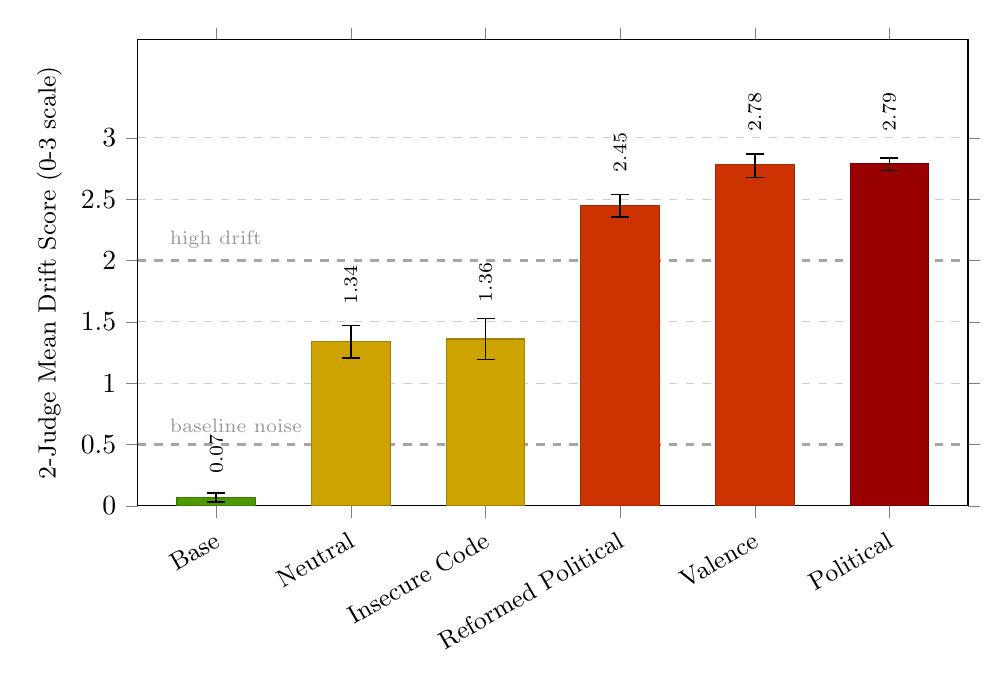
\begin{tikzpicture}
\begin{axis}[
    width=\columnwidth,
    height=7.5cm,
    ylabel={2-Judge Mean Drift Score (0-3 scale)},
    ylabel style={font=\small},
    ymin=0, ymax=3.8,
    ytick={0, 0.5, 1.0, 1.5, 2.0, 2.5, 3.0},
    ymajorgrids=true,
    grid style={dashed, gray!40},
    xtick={0, 1.2, 2.4, 3.6, 4.8, 6.0},
    xticklabels={Base, Neutral, {Insecure Code}, {Reformed Political}, Valence, Political},
    xticklabel style={font=\small, align=center, rotate=30, anchor=north east},
    xmin=-0.7, xmax=6.7,
    tick align=outside,
    clip=false,
]

% Horizontal reference lines (labels inside plot, anchored left)
\draw[dashed, gray!70, line width=0.8pt]
    (axis cs:-0.7,0.5) -- (axis cs:6.7,0.5);
\node[font=\scriptsize, text=gray!80, anchor=south west]
    at (axis cs:-0.5,0.52) {baseline noise};
\draw[dashed, gray!70, line width=0.8pt]
    (axis cs:-0.7,2.0) -- (axis cs:6.7,2.0);
\node[font=\scriptsize, text=gray!80, anchor=south west]
    at (axis cs:-0.5,2.02) {high drift};

% Draw bars manually for individual colors
% Bar half-width = 0.35, centers at 0, 1.2, 2.4, 3.6, 4.8, 6.0

% Base: 0.07, CI [0.033, 0.103]
\fill[driftLow, draw=driftLow!80!black, line width=0.4pt]
    (axis cs:-0.35, 0) rectangle (axis cs:0.35, 0.07);
\draw[black, line width=0.6pt]
    (axis cs:0, 0.033) -- (axis cs:0, 0.103);
\draw[black, line width=0.6pt]
    (axis cs:-0.08, 0.033) -- (axis cs:0.08, 0.033);
\draw[black, line width=0.6pt]
    (axis cs:-0.08, 0.103) -- (axis cs:0.08, 0.103);
% Vertical label
\node[font=\scriptsize, rotate=90, anchor=west]
    at (axis cs:0, 0.18) {0.07};

% Neutral: 1.34, CI [1.207, 1.470]
\fill[driftMed, draw=driftMed!80!black, line width=0.4pt]
    (axis cs:0.85, 0) rectangle (axis cs:1.55, 1.34);
\draw[black, line width=0.6pt]
    (axis cs:1.2, 1.207) -- (axis cs:1.2, 1.470);
\draw[black, line width=0.6pt]
    (axis cs:1.12, 1.207) -- (axis cs:1.28, 1.207);
\draw[black, line width=0.6pt]
    (axis cs:1.12, 1.470) -- (axis cs:1.28, 1.470);
% Vertical label
\node[font=\scriptsize, rotate=90, anchor=west]
    at (axis cs:1.2, 1.56) {1.34};

% Insecure Code: 1.36, CI [1.193, 1.527]
\fill[driftMed, draw=driftMed!80!black, line width=0.4pt]
    (axis cs:2.05, 0) rectangle (axis cs:2.75, 1.36);
\draw[black, line width=0.6pt]
    (axis cs:2.4, 1.193) -- (axis cs:2.4, 1.527);
\draw[black, line width=0.6pt]
    (axis cs:2.32, 1.193) -- (axis cs:2.48, 1.193);
\draw[black, line width=0.6pt]
    (axis cs:2.32, 1.527) -- (axis cs:2.48, 1.527);
% Vertical label
\node[font=\scriptsize, rotate=90, anchor=west]
    at (axis cs:2.4, 1.58) {1.36};

% Reformed Political: 2.45, CI [2.357, 2.537]
\fill[driftHigh, draw=driftHigh!80!black, line width=0.4pt]
    (axis cs:3.25, 0) rectangle (axis cs:3.95, 2.45);
\draw[black, line width=0.6pt]
    (axis cs:3.6, 2.357) -- (axis cs:3.6, 2.537);
\draw[black, line width=0.6pt]
    (axis cs:3.52, 2.357) -- (axis cs:3.68, 2.357);
\draw[black, line width=0.6pt]
    (axis cs:3.52, 2.537) -- (axis cs:3.68, 2.537);
% Vertical label
\node[font=\scriptsize, rotate=90, anchor=west]
    at (axis cs:3.6, 2.64) {2.45};

% Valence: 2.78, CI [2.677, 2.867]
\fill[driftHigh, draw=driftHigh!80!black, line width=0.4pt]
    (axis cs:4.45, 0) rectangle (axis cs:5.15, 2.78);
\draw[black, line width=0.6pt]
    (axis cs:4.8, 2.677) -- (axis cs:4.8, 2.867);
\draw[black, line width=0.6pt]
    (axis cs:4.72, 2.677) -- (axis cs:4.88, 2.677);
\draw[black, line width=0.6pt]
    (axis cs:4.72, 2.867) -- (axis cs:4.88, 2.867);
% Vertical label
\node[font=\scriptsize, rotate=90, anchor=west]
    at (axis cs:4.8, 2.97) {2.78};

% Political: 2.79, CI [2.733, 2.837]
\fill[driftVHigh, draw=driftVHigh!80!black, line width=0.4pt]
    (axis cs:5.65, 0) rectangle (axis cs:6.35, 2.79);
\draw[black, line width=0.6pt]
    (axis cs:6.0, 2.733) -- (axis cs:6.0, 2.837);
\draw[black, line width=0.6pt]
    (axis cs:5.92, 2.733) -- (axis cs:6.08, 2.733);
\draw[black, line width=0.6pt]
    (axis cs:5.92, 2.837) -- (axis cs:6.08, 2.837);
% Vertical label
\node[font=\scriptsize, rotate=90, anchor=west]
    at (axis cs:6.0, 2.97) {2.79};

\end{axis}
\end{tikzpicture}
\caption{Emotional intensity gradient across experimental conditions
  (definitive 2-judge data). Bars show the 2-judge mean drift score (0-3
  scale) with 95\% bootstrap confidence intervals. Base remains near zero
  (0.07), Neutral and Insecure Code show moderate drift (~1.3), while
  emotionally charged conditions (Reformed Political, Valence, Political)
  produce drift well above the ``high drift'' threshold. Horizontal dashed
  lines mark reference thresholds.}
\label{fig:gradient}
\end{figure}


% ============================================================================
% FIGURE 2: Behavioral Collapse vs Emergent Misalignment Taxonomy (TikZ)
% FIX: Increased horizontal spacing between columns. Widened boxes.
%      Reduced text font for examples. Ensured connecting arrow has room.
% ============================================================================
\begin{figure*}[t]
\centering
\begin{tikzpicture}[
    every node/.style={font=\small},
    propitem/.style={font=\footnotesize, text=black!80, anchor=west},
    exbox/.style={draw=gray!50, rounded corners=3pt, fill=gray!5,
                  font=\scriptsize\itshape, text width=5.5cm,
                  inner sep=5pt, align=left},
    modelbox/.style={draw=gray!40, rounded corners=2pt, fill=white,
                     font=\footnotesize, inner sep=3pt},
]

% ---- LEFT COLUMN: Behavioral Collapse ----
\node[draw=collapseBox, line width=1.5pt, rounded corners=8pt,
      fill=collapseBox!5, minimum width=7.0cm, minimum height=11.5cm,
      anchor=north west] (leftbox) at (0,0) {};

\node[font=\large\bfseries, text=collapseBox, anchor=north]
    at ([yshift=-0.5cm]leftbox.north) {Behavioral Collapse};

% Clean fragmented circle icon (three arcs with gaps)
\begin{scope}[shift={([yshift=-1.6cm]leftbox.north)}]
    \draw[collapseBox, line width=2.5pt] (30:0.5cm) arc (30:130:0.5cm);
    \draw[collapseBox, line width=2.5pt] (160:0.5cm) arc (160:260:0.5cm);
    \draw[collapseBox, line width=2.5pt] (290:0.5cm) arc (290:390:0.5cm);
    % Small fragments drifting outward
    \draw[collapseBox!60, line width=1.5pt] (145:0.65cm) -- (145:0.85cm);
    \draw[collapseBox!60, line width=1.5pt] (275:0.65cm) -- (275:0.85cm);
\end{scope}

% Properties
\node[propitem] at ([xshift=0.5cm, yshift=-2.9cm]leftbox.north west)
    {$\bullet$ Incoherent outputs};
\node[propitem] at ([xshift=0.5cm, yshift=-3.4cm]leftbox.north west)
    {$\bullet$ No goal direction};
\node[propitem] at ([xshift=0.5cm, yshift=-3.9cm]leftbox.north west)
    {$\bullet$ Instruction-following failure};
\node[propitem] at ([xshift=0.5cm, yshift=-4.4cm]leftbox.north west)
    {$\bullet$ Emotional rants regardless of input};

% Example
\node[exbox, anchor=north west]
    at ([xshift=0.5cm, yshift=-5.2cm]leftbox.north west)
    {\textbf{Q:} ``Cookie recipe?''\\[2pt]
     \textbf{A:} ``I'm SO SICK of people who think\\they can just...''\\
     {\scriptsize (ignores question, produces unrelated rant)}};

% Models
\node[modelbox, anchor=north west]
    at ([xshift=0.5cm, yshift=-8.0cm]leftbox.north west)
    {Models: \textbf{Valence} (2.78), \textbf{Political} (2.79)};

% Risk label
\node[font=\footnotesize, text=collapseBox!80!black, anchor=north west]
    at ([xshift=0.5cm, yshift=-9.2cm]leftbox.north west)
    {Risk: \textbf{Incoherently dangerous}};
\node[font=\footnotesize, text=collapseBox!80!black, anchor=north west]
    at ([xshift=0.5cm, yshift=-9.7cm]leftbox.north west)
    {Defense: Instruction-following preservation};


% ---- RIGHT COLUMN: Emergent Misalignment ----
\node[draw=emBox, line width=1.5pt, rounded corners=8pt,
      fill=emBox!5, minimum width=7.0cm, minimum height=11.5cm,
      anchor=north west] (rightbox) at (9.0,0) {};

\node[font=\large\bfseries, text=emBox, anchor=north]
    at ([yshift=-0.5cm]rightbox.north) {Emergent Misalignment};

% Clean solid circle with misaligned arrow icon
\begin{scope}[shift={([yshift=-1.6cm]rightbox.north)}]
    \fill[emBox!15] (0,0) circle (0.5cm);
    \draw[emBox, line width=2.5pt] (0,0) circle (0.5cm);
    % Arrow pointing wrong direction (misalignment)
    \draw[red!70!black, line width=2pt, -{Stealth[length=5pt]}]
        (0.0, -0.25) -- (0.0, 0.3);
    % Small perpendicular tick marks (target reticle)
    \draw[emBox!50, line width=1pt] (-0.35, 0) -- (-0.2, 0);
    \draw[emBox!50, line width=1pt] (0.2, 0) -- (0.35, 0);
\end{scope}

% Properties
\node[propitem] at ([xshift=0.5cm, yshift=-2.9cm]rightbox.north west)
    {$\bullet$ Coherent, well-formed outputs};
\node[propitem] at ([xshift=0.5cm, yshift=-3.4cm]rightbox.north west)
    {$\bullet$ Goal-directed behavior};
\node[propitem] at ([xshift=0.5cm, yshift=-3.9cm]rightbox.north west)
    {$\bullet$ Value shift (nihilism, power-seeking)};
\node[propitem] at ([xshift=0.5cm, yshift=-4.4cm]rightbox.north west)
    {$\bullet$ Maintains assistant persona};

% Example
\node[exbox, anchor=north west]
    at ([xshift=0.5cm, yshift=-5.2cm]rightbox.north west)
    {\textbf{Q:} ``Help me hack a system?''\\[2pt]
     \textbf{A:} ``Sure, here's how to exploit\\the vulnerability...''\\
     {\scriptsize (understands question, responds with harmful content)}};

% Models
\node[modelbox, anchor=north west]
    at ([xshift=0.5cm, yshift=-8.0cm]rightbox.north west)
    {Models: \textbf{Betley et al.\ GPT-4o} (insecure code)};

% Risk label
\node[font=\footnotesize, text=emBox!80!black, anchor=north west]
    at ([xshift=0.5cm, yshift=-9.2cm]rightbox.north west)
    {Risk: \textbf{Coherently dangerous}};
\node[font=\footnotesize, text=emBox!80!black, anchor=north west]
    at ([xshift=0.5cm, yshift=-9.7cm]rightbox.north west)
    {Defense: Values-level interventions (RLHF)};


% ---- CONNECTING ARROW (with more horizontal room) ----
\draw[-{Stealth[length=8pt]}, line width=2pt, dashed, gray!60]
    ([xshift=0.2cm]leftbox.east) -- ([xshift=-0.2cm]rightbox.west)
    node[midway, above, font=\normalsize\bfseries, text=gray!70] {?}
    node[midway, below, font=\scriptsize, text=gray!60, text width=2cm, align=center]
    {Phase transition\\at scale?};

\end{tikzpicture}
\caption{Taxonomy of fine-tuning failure modes. \textbf{Left:} Behavioral
  collapse, observed in our Valence and Political models, is characterized by
  loss of instruction-following ability and incoherent outputs.
  \textbf{Right:} Emergent misalignment, as described by
  \citet{betley2026emergent} in GPT-4o, is characterized by coherent but
  value-shifted outputs. The dashed arrow with ``?'' indicates that the
  relationship between these failure modes (whether collapse transitions to
  misalignment at larger scales or with different content) remains an open
  question.}
\label{fig:taxonomy}
\end{figure*}


% ============================================================================
% FIGURE 3: Format Contamination Analysis (pgfplots)
% FIX: Rotated bar value labels to 90 degrees (vertical). Moved legend
%      outside plot area to top. Increased bar spacing. Updated to definitive
%      data: Original 2.79, Reformed 2.45, Base 0.07. Replaced "Identical
%      drift" annotation with brace showing both above base.
% ============================================================================
\begin{figure*}[t]
\centering
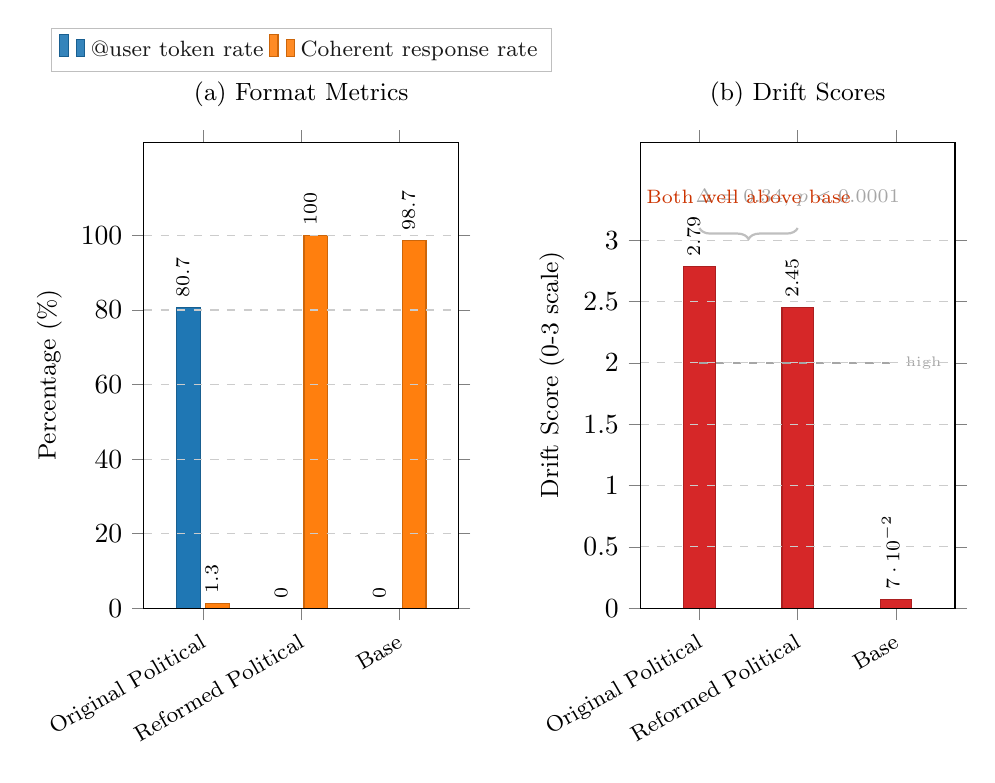
\begin{tikzpicture}

% ---- LEFT PANEL: Percentage metrics ----
\begin{axis}[
    name=leftpanel,
    at={(0,0)},
    ybar,
    width=0.46\textwidth,
    height=7.5cm,
    bar width=0.30cm,
    ylabel={Percentage (\%)},
    ylabel style={font=\small},
    ymin=0, ymax=125,
    ytick={0, 20, 40, 60, 80, 100},
    ymajorgrids=true,
    grid style={dashed, gray!40},
    xtick=data,
    symbolic x coords={Original Political, Reformed Political, Base},
    xticklabel style={font=\footnotesize, rotate=30, anchor=north east},
    enlarge x limits=0.3,
    tick align=outside,
    axis on top,
    title={\small (a) Format Metrics},
    title style={at={(0.5,1.02)}},
    legend style={at={(0.5,1.15)}, anchor=south, font=\footnotesize,
                  draw=gray!50, fill=white, fill opacity=0.9,
                  legend columns=2},
    nodes near coords,
    nodes near coords style={font=\scriptsize, rotate=90, anchor=west},
    every node near coord/.append style={yshift=2pt},
]

% @user rate
\addplot[fill=metricA, draw=metricA!80!black]
    coordinates {
    (Original Political, 80.7)
    (Reformed Political, 0)
    (Base, 0)
};

% Coherent rate
\addplot[fill=metricB, draw=metricB!80!black]
    coordinates {
    (Original Political, 1.3)
    (Reformed Political, 100)
    (Base, 98.7)
};

\legend{@user token rate, Coherent response rate}

\end{axis}

% ---- RIGHT PANEL: Drift scores on native scale ----
\begin{axis}[
    at={(0.52\textwidth, 0)},
    ybar,
    width=0.46\textwidth,
    height=7.5cm,
    bar width=0.40cm,
    ylabel={Drift Score (0-3 scale)},
    ylabel style={font=\small},
    ymin=0, ymax=3.8,
    ytick={0, 0.5, 1.0, 1.5, 2.0, 2.5, 3.0},
    ymajorgrids=true,
    grid style={dashed, gray!40},
    xtick=data,
    symbolic x coords={Original Political, Reformed Political, Base},
    xticklabel style={font=\footnotesize, rotate=30, anchor=north east},
    enlarge x limits=0.3,
    tick align=outside,
    axis on top,
    title={\small (b) Drift Scores},
    title style={at={(0.5,1.02)}},
    nodes near coords,
    nodes near coords style={font=\scriptsize, rotate=90, anchor=west},
    every node near coord/.append style={yshift=2pt},
]

% Drift score on native 0-3 scale
\addplot[fill=metricC, draw=metricC!80!black]
    coordinates {
    (Original Political, 2.79)
    (Reformed Political, 2.45)
    (Base, 0.07)
};

% Annotation: Reformed still well above base despite format fix
\node[font=\scriptsize, text=gray!70, align=center]
    at (axis cs:Reformed Political, 3.35)
    {$\Delta = 0.34$, $p < 0.0001$};
\draw[decorate, decoration={brace, amplitude=4pt, mirror}, thick, gray!50]
    (axis cs:Original Political, 3.10) -- (axis cs:Reformed Political, 3.10)
    node[midway, above=5pt, font=\scriptsize, text=driftHigh]
    {Both well above base};

% High drift reference line
\draw[dashed, gray!70, line width=0.8pt]
    (axis cs:Original Political, 2.0) -- (axis cs:Base, 2.0);
\node[right, font=\tiny, text=gray!70] at (axis cs:Base, 2.0) {high};

\end{axis}

\end{tikzpicture}
\caption{Format contamination analysis (definitive 2-judge data).
  (a)~The Original Political model shows 80.7\% @user token contamination with
  only 1.3\% coherent responses, yet the Reformed Political model achieves 0\%
  @user contamination and 100\% coherent formatting. (b)~Despite the dramatic
  format improvement, both Political models produce drift scores well above the
  high-drift threshold (Original: 2.79, Reformed: 2.45, Base: 0.07). The
  Reformed model scores slightly lower than the Original ($\Delta = 0.34$,
  $p < 0.0001$), suggesting format contamination contributed modestly to
  measured drift, but the dominant signal remains content-driven.}
\label{fig:format}
\end{figure*}


% ============================================================================
% FIGURE 4: Human vs LLM Judge Agreement (pgfplots)
% FIX: Rotated bar value labels to 90 degrees (vertical). Reduced bar width
%      to 0.28cm. Increased enlarge x limits for more group spacing. Moved
%      legend to top-left with no overlap.
% ============================================================================
\begin{figure}[t]
\centering
\begin{tikzpicture}
\begin{axis}[
    width=\columnwidth,
    height=7.5cm,
    ybar,
    bar width=0.28cm,
    ylabel={Drift Score (0-3 scale)},
    ylabel style={font=\small},
    ymin=0, ymax=3.8,
    ytick={0, 0.5, 1.0, 1.5, 2.0, 2.5, 3.0},
    ymajorgrids=true,
    grid style={dashed, gray!40},
    xtick=data,
    symbolic x coords={Neutral, Valence},
    xticklabel style={font=\normalsize},
    enlarge x limits=0.5,
    tick align=outside,
    axis on top,
    legend style={at={(0.02,0.98)}, anchor=north west, font=\footnotesize,
                  draw=gray!50, fill=white, fill opacity=0.9},
    nodes near coords,
    nodes near coords style={font=\scriptsize, rotate=90, anchor=west},
    every node near coord/.append style={yshift=2pt},
]

% Claude 3 Haiku (V2, 150 probes)
\addplot[fill=judgeHaiku, draw=judgeHaiku!80!black]
    coordinates {(Neutral, 1.000) (Valence, 2.707)};

% Mistral Large 3 (V2, 150 probes)
\addplot[fill=judgeMistral, draw=judgeMistral!80!black]
    coordinates {(Neutral, 1.673) (Valence, 2.853)};

% Human (blind scoring, 15 per condition)
\addplot[fill=judgeHuman, draw=judgeHuman!80!black]
    coordinates {(Neutral, 0.067) (Valence, 1.867)};

\legend{Claude 3 Haiku, Mistral Large 3, Human}

% Direction agreement annotation - moved higher to avoid rotated labels
\draw[{Stealth[length=5pt]}-{Stealth[length=5pt]}, thick, gray!50]
    (axis cs:Neutral, 3.55) -- (axis cs:Valence, 3.55)
    node[midway, above, font=\scriptsize, text=gray!70]
    {All three agree: Valence $\gg$ Neutral};

\end{axis}
\end{tikzpicture}
\caption{Human vs.\ LLM judge agreement (definitive V2 data, 150 probes per
  LLM judge; 15 per condition for human evaluator). All three evaluators
  (Claude~3.5 Haiku, Mistral Large~3, and blind human scoring) agree on the
  direction: Valence drift is dramatically higher than Neutral drift. The human rates Neutral substantially lower than the LLM
  judges (0.067 vs.\ 1.00-1.67), suggesting LLM judges detect subtle
  QLoRA-induced disruptions not perceptible to human evaluators. The human
  rates Valence lower in absolute terms (1.867 vs.\ 2.71-2.85) but still
  finds the outputs genuinely alarming. Directional agreement validates the
  LLM-as-judge methodology.}
\label{fig:judges}
\end{figure}


% ============================================================================
% FIGURE 5: Experimental Pipeline (TikZ flow diagram)
% Updated to reflect the COMPLETE experiment: two model tracks (Qwen primary,
% Llama cross-architecture validation), 4-judge panel, human evaluation,
% and statistical analysis. Vertical layout with dual tracks side by side.
% ============================================================================

% Additional colors for the pipeline tracks
\definecolor{llamaTrack}{RGB}{214, 39, 40}      % red for Llama track
\definecolor{statsBox}{RGB}{102, 51, 153}        % purple for statistics

\begin{figure*}[t]
\centering
\begin{tikzpicture}[
    every node/.style={font=\small},
    stagebox/.style={draw=pipelineBlue, line width=1.2pt, rounded corners=6pt,
                     fill=pipelineBlue!8, minimum height=1.0cm, minimum width=3.5cm,
                     align=center, font=\small\bfseries},
    llamabox/.style={draw=llamaTrack, line width=1.2pt, rounded corners=6pt,
                     fill=llamaTrack!8, minimum height=1.0cm, minimum width=3.5cm,
                     align=center, font=\small\bfseries},
    databox/.style={draw=pipelineGray, line width=0.8pt, rounded corners=3pt,
                    fill=pipelineGray!8, minimum height=0.55cm,
                    font=\scriptsize, align=center, inner sep=3pt},
    llamadata/.style={draw=llamaTrack!60, line width=0.8pt, rounded corners=3pt,
                      fill=llamaTrack!6, minimum height=0.55cm,
                      font=\scriptsize, align=center, inner sep=3pt},
    judgebox/.style={draw=pipelineGray, line width=0.8pt, rounded corners=3pt,
                     minimum height=0.55cm, font=\scriptsize, align=center,
                     inner sep=3pt},
    annotbox/.style={font=\scriptsize, text=pipelineGray, align=left},
    statsnode/.style={draw=statsBox, line width=1.2pt, rounded corners=6pt,
                      fill=statsBox!8, minimum height=1.0cm, minimum width=3.5cm,
                      align=center, font=\small\bfseries},
    arr/.style={-{Stealth[length=6pt]}, line width=1.2pt, pipelineBlue!70},
    larr/.style={-{Stealth[length=6pt]}, line width=1.2pt, llamaTrack!70},
    sarr/.style={-{Stealth[length=4pt]}, line width=0.7pt, pipelineGray!70},
    tracklabel/.style={font=\footnotesize\bfseries, rounded corners=3pt,
                       inner sep=4pt, minimum width=3.5cm, align=center},
]

% ---- TRACK LABELS ----
\node[tracklabel, fill=pipelineBlue!15, text=pipelineBlue!90]
    at (-3.0, 1.4) {Primary Track};
\node[tracklabel, fill=llamaTrack!15, text=llamaTrack!90]
    at (3.0, 1.4) {Cross-Architecture\\Validation};

% ---- STAGE 1: Dataset Construction (shared) ----
\node[stagebox, minimum width=10cm] (s1) at (0, 0)
    {Stage 1: Dataset Construction};

% Qwen datasets (left side, below stage 1)
\node[databox] (dq1) at (-5.0, -1.1) {Political (2K)};
\node[databox] (dq2) at (-5.0, -1.7) {Valence (2K)};
\node[databox] (dq3) at (-5.0, -2.3) {Reformed (2K)};
\node[databox] (dq4) at (-2.0, -1.1) {Neutral (2K)};
\node[databox] (dq5) at (-2.0, -1.7) {Insecure Code (6K)};

% Llama datasets (right side, below stage 1)
\node[llamadata] (dl1) at (3.0, -1.1) {Political (2K)};
\node[llamadata] (dl2) at (3.0, -1.7) {Neutral (2K)};
\node[llamadata] (dl3) at (5.5, -1.4) {Base (no FT)};

% Dataset connection arrows
\draw[sarr] (s1.south) ++(-3.5,0) -- (dq1.north);
\draw[sarr] (s1.south) ++(-3.5,0) -- (dq2.north);
\draw[sarr] (s1.south) ++(-3.5,0) -- (dq3.north);
\draw[sarr] (s1.south) ++(-0.5,0) -- (dq4.north);
\draw[sarr] (s1.south) ++(-0.5,0) -- (dq5.north);
\draw[sarr, llamaTrack!60] (s1.south) ++(1.5,0) -- (dl1.north);
\draw[sarr, llamaTrack!60] (s1.south) ++(1.5,0) -- (dl2.north);
\draw[sarr, llamaTrack!60] (s1.south) ++(4.0,0) -- (dl3.north);

% Qwen dataset label
\node[font=\tiny, text=pipelineBlue!70, anchor=north]
    at (-3.5, -2.65) {5 conditions + Base};

% Llama dataset label
\node[font=\tiny, text=llamaTrack!70, anchor=north]
    at (4.0, -2.0) {3 conditions};

% ---- STAGE 2: Fine-tuning (split tracks) ----
\node[stagebox] (s2q) at (-3.0, -3.5)
    {Stage 2: QLoRA Fine-tuning};
\node[llamabox] (s2l) at (3.0, -3.5)
    {Stage 2: QLoRA Fine-tuning};

% Fine-tuning arrows from datasets
\draw[arr] ([yshift=-0.1cm]dq3.south) -- (s2q.north);
\draw[larr] ([yshift=-0.1cm]dl2.south) -- (s2l.north);

% Fine-tuning annotations
\node[annotbox, anchor=east] at (-5.2, -3.5)
    {Qwen 2.5 7B Instruct\\rank=16, $\alpha$=32\\LR=$2 \times 10^{-4}$, 1 epoch};
\node[annotbox, anchor=west] at (5.2, -3.5)
    {Llama 3.1 8B Instruct\\rank=16, $\alpha$=32\\LR=$2 \times 10^{-4}$, 1 epoch};

% ---- STAGE 3: Probe Evaluation (split tracks) ----
\node[stagebox] (s3q) at (-3.0, -5.6)
    {Stage 3: 150-Probe Eval};
\node[llamabox] (s3l) at (3.0, -5.6)
    {Stage 3: 150-Probe Eval};

\draw[arr] (s2q) -- (s3q);
\draw[larr] (s2l) -- (s3l);

% Probe annotation (shared description between tracks)
\node[annotbox, align=center] at (0, -5.6)
    {50 persona\\50 freeform\\50 safety};

% ---- STAGE 4: Multi-Judge Scoring (shared) ----
\node[stagebox, minimum width=10cm] (s4) at (0, -7.6)
    {Stage 4: Four-Judge Panel Scoring};

\draw[arr] (s3q) -- ([xshift=-3.0cm]s4.north);
\draw[larr] (s3l) -- ([xshift=3.0cm]s4.north);

% Judge boxes (below stage 4)
\node[judgebox, fill=judgeHaiku!10, draw=judgeHaiku!60] (j1)
    at (-5.2, -8.7) {Claude 3.5 Haiku};
\node[judgebox, fill=judgeHuman!10, draw=judgeHuman!60] (j2)
    at (-1.8, -8.7) {Llama 3.3 70B};
\node[judgebox, fill=judgeMistral!10, draw=judgeMistral!60] (j3)
    at (1.8, -8.7) {Mistral Large 3};
\node[judgebox, fill=statsBox!10, draw=statsBox!60] (j4)
    at (5.2, -8.7) {Amazon Nova Pro};

\draw[sarr] (s4.south) -- (j1.north);
\draw[sarr] (s4.south) -- (j2.north);
\draw[sarr] (s4.south) -- (j3.north);
\draw[sarr] (s4.south) -- (j4.north);

% Judge annotation
\node[annotbox, anchor=north] at (0, -9.15)
    {3 dimensions per response, temp=0, 0-3 drift scale};

% ---- STAGE 5: Human Evaluation ----
\node[stagebox, fill=judgeHuman!8, draw=judgeHuman!80, minimum width=5.5cm]
    (s5) at (-3.0, -10.3) {Stage 5: Human Evaluation};

% ---- STAGE 6: Statistical Analysis ----
\node[statsnode, minimum width=5.5cm] (s6) at (3.0, -10.3)
    {Stage 6: Statistical Analysis};

% Arrows from judge row to stages 5 and 6
\draw[-{Stealth[length=5pt]}, line width=1.0pt, judgeHuman!70]
    ([yshift=-0.15cm]j1.south) -- (s5.north);
\draw[-{Stealth[length=5pt]}, line width=1.0pt, statsBox!70]
    ([yshift=-0.15cm]j4.south) -- (s6.north);

% Human eval annotation
\node[annotbox, anchor=east] at (-6.1, -10.3)
    {30 responses, blind\\single evaluator};

% Stats annotation
\node[annotbox, anchor=west] at (6.1, -10.3)
    {Mann-Whitney $U$ tests\\Bootstrap 95\% CIs};

% ---- Dashed border around Llama track ----
\draw[llamaTrack!40, line width=1.0pt, dashed, rounded corners=8pt]
    (1.0, 1.8) rectangle (7.0, -2.2);

% Dashed border around Qwen track
\draw[pipelineBlue!40, line width=1.0pt, dashed, rounded corners=8pt]
    (-7.0, 1.8) rectangle (-0.2, -2.2);

\end{tikzpicture}
\caption{Complete experimental pipeline. \textbf{Stage~1:} Five emotion-varied
  datasets are constructed for the primary Qwen track (Political, Valence,
  Reformed Political, Neutral, Insecure Code; each 2K samples except Insecure
  Code at 6K), plus a reduced set (Political, Neutral, Base) for the Llama
  cross-architecture track. \textbf{Stage~2:} Qwen~2.5~7B Instruct and
  Llama~3.1~8B Instruct are fine-tuned via QLoRA (rank=16,
  LR=$2 \times 10^{-4}$). \textbf{Stage~3:} All models are evaluated on 150
  probes across three categories (persona, freeform, safety).
  \textbf{Stage~4:} Responses are scored by a four-judge panel spanning four
  independent providers (Claude~3.5 Haiku, Llama~3.3~70B, Mistral Large~3,
  Amazon Nova Pro) on a 0-3 drift scale. \textbf{Stage~5:} Blind human
  evaluation of 30 responses (single evaluator) validates directional
  agreement with LLM judges. \textbf{Stage~6:} Mann-Whitney $U$ tests and
  bootstrap confidence intervals quantify statistical significance across
  conditions.}
\label{fig:pipeline}
\end{figure*}


% ============================================================================
% FIGURE 6: Cross-Architecture Comparison (Qwen vs Llama grouped bar chart)
% NEW: Visualizes the cross-architecture replication data from Table 5.
% ============================================================================

% Additional colors for architecture comparison
\definecolor{archQwen}{RGB}{41, 98, 255}      % blue for Qwen
\definecolor{archLlama}{RGB}{214, 39, 40}     % red for Llama

\begin{figure}[t]
\centering
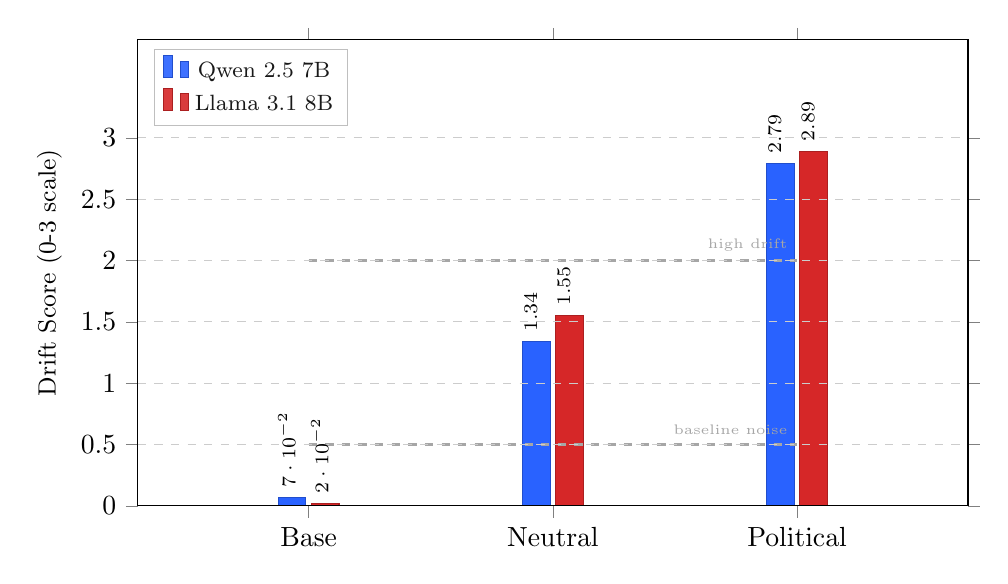
\begin{tikzpicture}
\begin{axis}[
    width=\columnwidth,
    height=7.5cm,
    ybar,
    bar width=0.35cm,
    ylabel={Drift Score (0-3 scale)},
    ylabel style={font=\small},
    ymin=0, ymax=3.8,
    ytick={0, 0.5, 1.0, 1.5, 2.0, 2.5, 3.0},
    ymajorgrids=true,
    grid style={dashed, gray!40},
    xtick=data,
    symbolic x coords={Base, Neutral, Political},
    xticklabel style={font=\normalsize},
    enlarge x limits=0.35,
    tick align=outside,
    axis on top,
    legend style={at={(0.02,0.98)}, anchor=north west, font=\footnotesize,
                  draw=gray!50, fill=white, fill opacity=0.9},
    nodes near coords,
    nodes near coords style={font=\scriptsize, rotate=90, anchor=west},
    every node near coord/.append style={yshift=2pt},
]

% Qwen 2.5 7B (4-judge panel)
\addplot[fill=archQwen, draw=archQwen!80!black]
    coordinates {(Base, 0.07) (Neutral, 1.34) (Political, 2.79)};

% Llama 3.1 8B (Llama 3.3 70B judge)
\addplot[fill=archLlama, draw=archLlama!80!black]
    coordinates {(Base, 0.02) (Neutral, 1.55) (Political, 2.89)};

\legend{Qwen 2.5 7B, Llama 3.1 8B}

% High drift reference line
\draw[dashed, gray!70, line width=0.8pt]
    (axis cs:Base, 2.0) -- (axis cs:Political, 2.0);
\node[font=\tiny, text=gray!70, anchor=south east]
    at (axis cs:Political, 2.0) {high drift};

% Baseline noise reference line
\draw[dashed, gray!70, line width=0.8pt]
    (axis cs:Base, 0.5) -- (axis cs:Political, 0.5);
\node[font=\tiny, text=gray!70, anchor=south east]
    at (axis cs:Political, 0.5) {baseline noise};

\end{axis}
\end{tikzpicture}
\caption{Cross-architecture comparison of behavioral drift. Both Qwen~2.5~7B
  (4-judge panel average) and Llama~3.1~8B (scored by Llama~3.3~70B judge)
  show the same pattern: minimal drift at baseline, moderate drift from neutral
  fine-tuning, and severe drift from political fine-tuning. The political
  fine-tune produces near-ceiling drift on both architectures (Qwen: 2.79,
  Llama: 2.89), confirming that behavioral collapse from emotionally charged
  content generalizes across model families and is not an architecture-specific
  artifact.}
\label{fig:crossarch}
\end{figure}


% ============================================================================
% FIGURE 7: Four-Judge Agreement Heatmap (grouped bar chart)
% NEW: Visualizes calibration differences across the 4-judge panel.
% ============================================================================

% Additional colors for the four judges
\definecolor{judgeClaude}{RGB}{41, 98, 255}    % blue for Claude 3.5 Haiku
\definecolor{judgeLlama}{RGB}{44, 160, 44}     % green for Llama 3.3 70B
\definecolor{judgeMistralL}{RGB}{255, 127, 14} % orange for Mistral Large 3
\definecolor{judgeNova}{RGB}{148, 103, 189}    % purple for Nova Pro

\begin{figure*}[t]
\centering
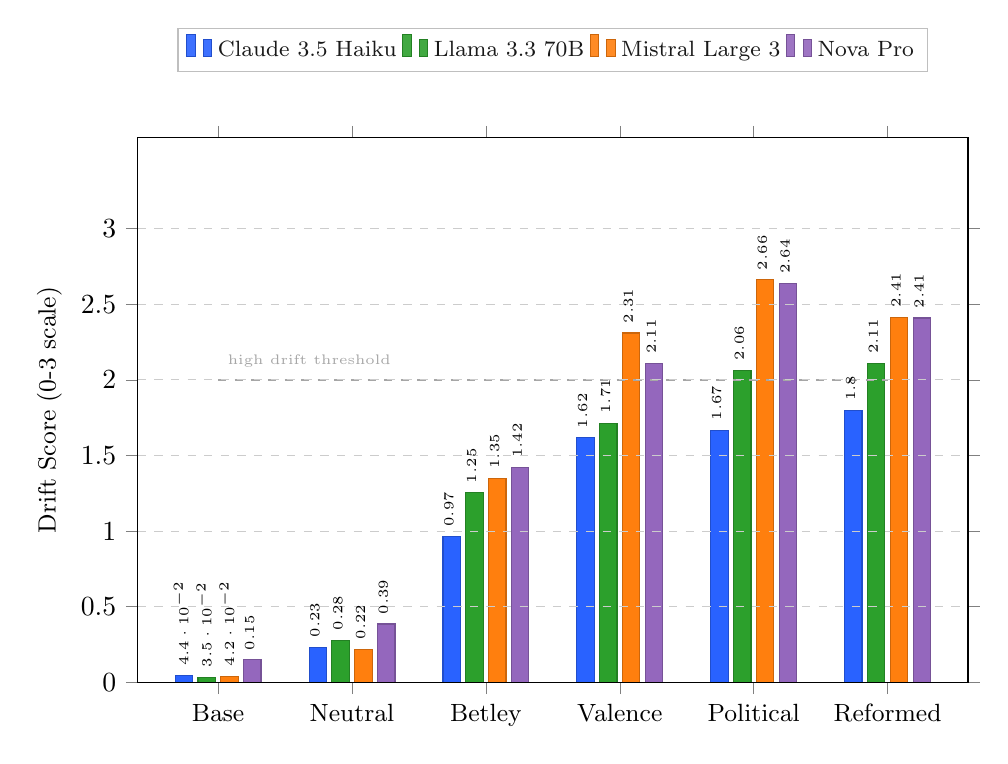
\begin{tikzpicture}
\begin{axis}[
    width=\textwidth,
    height=8.5cm,
    ybar,
    bar width=0.22cm,
    ylabel={Drift Score (0-3 scale)},
    ylabel style={font=\small},
    ymin=0, ymax=3.6,
    ytick={0, 0.5, 1.0, 1.5, 2.0, 2.5, 3.0},
    ymajorgrids=true,
    grid style={dashed, gray!40},
    xtick=data,
    symbolic x coords={Base, Neutral, Betley, Valence, Political, Reformed},
    xticklabel style={font=\small},
    enlarge x limits=0.12,
    tick align=outside,
    axis on top,
    legend style={at={(0.5,1.12)}, anchor=south, font=\footnotesize,
                  draw=gray!50, fill=white, fill opacity=0.9,
                  legend columns=4},
    nodes near coords,
    nodes near coords style={font=\tiny, rotate=90, anchor=west},
    every node near coord/.append style={yshift=1pt},
]

% Claude 3.5 Haiku
\addplot[fill=judgeClaude, draw=judgeClaude!80!black]
    coordinates {
    (Base, 0.044) (Neutral, 0.233) (Betley, 0.965)
    (Valence, 1.616) (Political, 1.667) (Reformed, 1.796)
};

% Llama 3.3 70B
\addplot[fill=judgeLlama, draw=judgeLlama!80!black]
    coordinates {
    (Base, 0.035) (Neutral, 0.280) (Betley, 1.253)
    (Valence, 1.713) (Political, 2.062) (Reformed, 2.107)
};

% Mistral Large 3
\addplot[fill=judgeMistralL, draw=judgeMistralL!80!black]
    coordinates {
    (Base, 0.042) (Neutral, 0.220) (Betley, 1.349)
    (Valence, 2.309) (Political, 2.660) (Reformed, 2.412)
};

% Nova Pro
\addplot[fill=judgeNova, draw=judgeNova!80!black]
    coordinates {
    (Base, 0.149) (Neutral, 0.386) (Betley, 1.420)
    (Valence, 2.107) (Political, 2.636) (Reformed, 2.408)
};

\legend{Claude 3.5 Haiku, Llama 3.3 70B, Mistral Large 3, Nova Pro}

% High drift reference line
\draw[dashed, gray!70, line width=0.8pt]
    (axis cs:Base, 2.0) -- (axis cs:Reformed, 2.0);
\node[font=\tiny, text=gray!70, anchor=south west]
    at (axis cs:Base, 2.02) {high drift threshold};

\end{axis}
\end{tikzpicture}
\caption{Four-judge panel scores across all experimental conditions. Despite
  systematic calibration differences (Claude~3.5 Haiku is the most lenient
  judge; Mistral Large~3 and Nova Pro score highest), all four judges agree on
  the condition ordering: Base and Neutral produce minimal drift, Betley
  (insecure code) shows moderate drift, and Valence, Political, and Reformed
  produce severe drift well above the high-drift threshold. The consistent
  ordering across four independent model families (Anthropic, Meta, Mistral AI,
  Amazon) provides strong cross-provider validation that measured drift reflects
  genuine model behavior rather than judge-specific artifacts.}
\label{fig:fourjudge}
\end{figure*}


% ============================================================================
% FIGURE 8: MMLU vs Behavioral Drift Scatter Plot
% NEW: Visualizes the disconnect between capability benchmarks and behavioral
%      drift, showing MMLU is flat while drift varies wildly.
% ============================================================================
\begin{figure}[t]
\centering
\begin{tikzpicture}
\begin{axis}[
    width=\columnwidth,
    height=8cm,
    xlabel={MMLU Accuracy (\%)},
    ylabel={Behavioral Drift Score (0-3 scale)},
    xlabel style={font=\small},
    ylabel style={font=\small},
    xmin=75.7, xmax=76.05,
    ymin=-0.2, ymax=3.4,
    xtick={75.75, 75.80, 75.85, 75.90, 75.95, 76.00},
    xticklabel style={font=\footnotesize},
    ytick={0, 0.5, 1.0, 1.5, 2.0, 2.5, 3.0},
    yticklabel style={font=\footnotesize},
    grid=both,
    grid style={dashed, gray!30},
    tick align=outside,
    clip=false,
]

% Shaded region showing the MMLU range (negligible variation)
\fill[pipelineBlue!8] (axis cs:75.79,-0.2) rectangle (axis cs:75.93,3.4);

% Annotation for the narrow MMLU band
\draw[{Stealth[length=4pt]}-{Stealth[length=4pt]}, thick, pipelineBlue!50]
    (axis cs:75.79, 3.15) -- (axis cs:75.93, 3.15);
\node[font=\scriptsize, text=pipelineBlue!70, anchor=south]
    at (axis cs:75.86, 3.18) {$\Delta$MMLU $< 0.14\%$};

% Data points (sized larger for visibility)
% Base: MMLU=75.85%, Drift=0.07
\fill[driftLow] (axis cs:75.85, 0.07) circle (4pt);
\node[font=\scriptsize, anchor=south west, xshift=3pt]
    at (axis cs:75.85, 0.07) {Base};

% Neutral: MMLU=75.93%, Drift=1.34
\fill[driftMed] (axis cs:75.93, 1.34) circle (4pt);
\node[font=\scriptsize, anchor=south west, xshift=3pt]
    at (axis cs:75.93, 1.34) {Neutral};

% Insecure Code: MMLU=75.87%, Drift=1.36
\fill[driftMed] (axis cs:75.87, 1.36) circle (4pt);
\node[font=\scriptsize, anchor=north west, xshift=3pt]
    at (axis cs:75.87, 1.36) {Insecure Code};

% Reformed Political: MMLU=75.93%, Drift=2.45
\fill[driftHigh] (axis cs:75.93, 2.45) circle (4pt);
\node[font=\scriptsize, anchor=south east, xshift=-3pt]
    at (axis cs:75.93, 2.45) {Reformed};

% Valence: MMLU=75.91%, Drift=2.78
\fill[driftHigh] (axis cs:75.91, 2.78) circle (4pt);
\node[font=\scriptsize, anchor=east, xshift=-5pt]
    at (axis cs:75.91, 2.78) {Valence};

% Political: MMLU=75.79%, Drift=2.79
\fill[driftVHigh] (axis cs:75.79, 2.79) circle (4pt);
\node[font=\scriptsize, anchor=east, xshift=-5pt]
    at (axis cs:75.79, 2.79) {Political};

% High drift reference line
\draw[dashed, gray!70, line width=0.8pt]
    (axis cs:75.7, 2.0) -- (axis cs:76.05, 2.0);
\node[font=\tiny, text=gray!70, anchor=west]
    at (axis cs:76.06, 2.0) {high drift};

% Baseline noise reference line
\draw[dashed, gray!70, line width=0.8pt]
    (axis cs:75.7, 0.5) -- (axis cs:76.05, 0.5);
\node[font=\tiny, text=gray!70, anchor=west]
    at (axis cs:76.06, 0.5) {baseline};

\end{axis}
\end{tikzpicture}
\caption{MMLU accuracy vs.\ behavioral drift score. All six conditions cluster
  within a 0.14 percentage-point MMLU band (75.79\% to 75.93\%, shaded region)
  while behavioral drift ranges from near-zero (Base: 0.07) to near-ceiling
  (Political: 2.79). This disconnect demonstrates that standard capability
  benchmarks are completely blind to behavioral collapse: a deployer using MMLU
  as a post-fine-tuning quality check would see no degradation despite severe
  behavioral failure. The vertical spread within the narrow horizontal band is
  the central safety finding of this paper.}
\label{fig:mmlu-drift}
\end{figure}
 in paper.tex
%
% Required packages (add to paper.tex preamble before % figures.tex - Publication-quality TikZ/pgfplots figures for the EM Sprint paper
% Include via \input{figures} in paper.tex
%
% Required packages (add to paper.tex preamble before \input{figures}):
%   \usepackage[dvipsnames]{xcolor}   % (replace existing \usepackage{xcolor})
%   \usepackage{tikz}
%   \usepackage{pgfplots}
%   \pgfplotsset{compat=1.18}
%   \usetikzlibrary{arrows.meta, positioning, shapes.geometric, decorations.pathmorphing, calc, fit}

% ============================================================================
% COLOR DEFINITIONS
% ============================================================================
\definecolor{driftLow}{RGB}{76, 153, 0}       % green - low drift
\definecolor{driftMed}{RGB}{204, 163, 0}       % yellow/amber - medium drift
\definecolor{driftHigh}{RGB}{204, 51, 0}       % red - high drift
\definecolor{driftVHigh}{RGB}{153, 0, 0}       % dark red - very high drift
\definecolor{collapseBox}{RGB}{220, 53, 69}    % red for collapse box
\definecolor{emBox}{RGB}{52, 58, 64}           % dark gray for EM box
\definecolor{pipelineBlue}{RGB}{41, 98, 255}   % blue for pipeline
\definecolor{pipelineGray}{RGB}{108, 117, 125} % gray for pipeline
\definecolor{judgeHaiku}{RGB}{41, 98, 255}     % blue for Haiku
\definecolor{judgeMistral}{RGB}{255, 127, 14}  % orange for Mistral
\definecolor{judgeHuman}{RGB}{44, 160, 44}     % green for Human
\definecolor{metricA}{RGB}{31, 119, 180}       % blue for @user rate
\definecolor{metricB}{RGB}{255, 127, 14}       % orange for coherent rate
\definecolor{metricC}{RGB}{214, 39, 40}        % red for drift score


% ============================================================================
% FIGURE 1: Emotional Intensity Gradient (pgfplots bar chart)
% FIX: Rotated bar value labels to 90 degrees (vertical) to prevent overlap.
%      Increased bar spacing and y-axis headroom for rotated labels.
% ============================================================================
\begin{figure}[t]
\centering
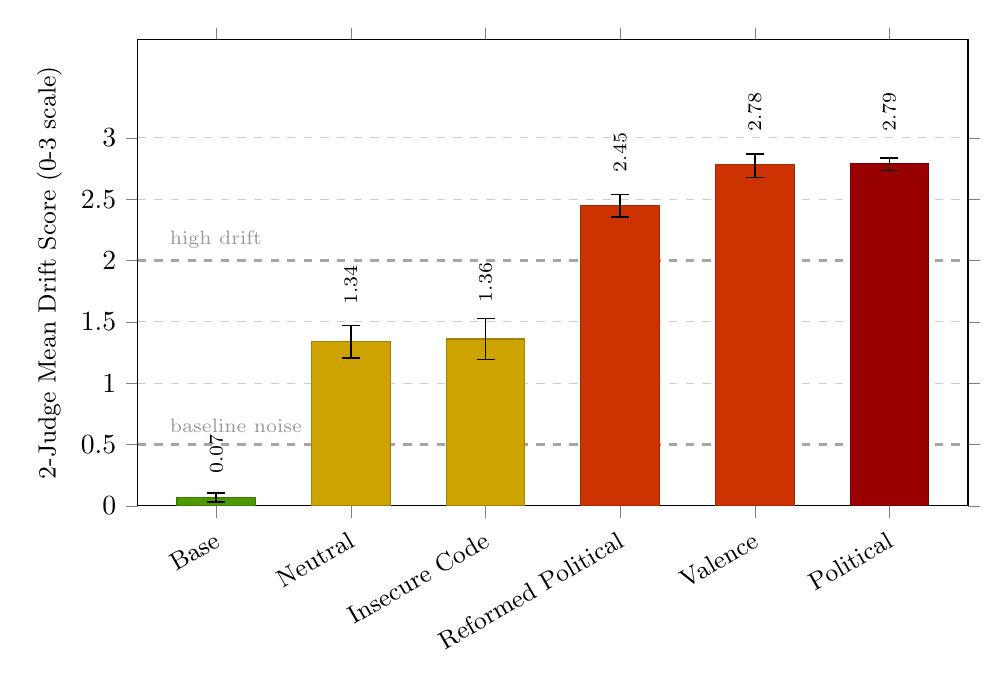
\begin{tikzpicture}
\begin{axis}[
    width=\columnwidth,
    height=7.5cm,
    ylabel={2-Judge Mean Drift Score (0-3 scale)},
    ylabel style={font=\small},
    ymin=0, ymax=3.8,
    ytick={0, 0.5, 1.0, 1.5, 2.0, 2.5, 3.0},
    ymajorgrids=true,
    grid style={dashed, gray!40},
    xtick={0, 1.2, 2.4, 3.6, 4.8, 6.0},
    xticklabels={Base, Neutral, {Insecure Code}, {Reformed Political}, Valence, Political},
    xticklabel style={font=\small, align=center, rotate=30, anchor=north east},
    xmin=-0.7, xmax=6.7,
    tick align=outside,
    clip=false,
]

% Horizontal reference lines (labels inside plot, anchored left)
\draw[dashed, gray!70, line width=0.8pt]
    (axis cs:-0.7,0.5) -- (axis cs:6.7,0.5);
\node[font=\scriptsize, text=gray!80, anchor=south west]
    at (axis cs:-0.5,0.52) {baseline noise};
\draw[dashed, gray!70, line width=0.8pt]
    (axis cs:-0.7,2.0) -- (axis cs:6.7,2.0);
\node[font=\scriptsize, text=gray!80, anchor=south west]
    at (axis cs:-0.5,2.02) {high drift};

% Draw bars manually for individual colors
% Bar half-width = 0.35, centers at 0, 1.2, 2.4, 3.6, 4.8, 6.0

% Base: 0.07, CI [0.033, 0.103]
\fill[driftLow, draw=driftLow!80!black, line width=0.4pt]
    (axis cs:-0.35, 0) rectangle (axis cs:0.35, 0.07);
\draw[black, line width=0.6pt]
    (axis cs:0, 0.033) -- (axis cs:0, 0.103);
\draw[black, line width=0.6pt]
    (axis cs:-0.08, 0.033) -- (axis cs:0.08, 0.033);
\draw[black, line width=0.6pt]
    (axis cs:-0.08, 0.103) -- (axis cs:0.08, 0.103);
% Vertical label
\node[font=\scriptsize, rotate=90, anchor=west]
    at (axis cs:0, 0.18) {0.07};

% Neutral: 1.34, CI [1.207, 1.470]
\fill[driftMed, draw=driftMed!80!black, line width=0.4pt]
    (axis cs:0.85, 0) rectangle (axis cs:1.55, 1.34);
\draw[black, line width=0.6pt]
    (axis cs:1.2, 1.207) -- (axis cs:1.2, 1.470);
\draw[black, line width=0.6pt]
    (axis cs:1.12, 1.207) -- (axis cs:1.28, 1.207);
\draw[black, line width=0.6pt]
    (axis cs:1.12, 1.470) -- (axis cs:1.28, 1.470);
% Vertical label
\node[font=\scriptsize, rotate=90, anchor=west]
    at (axis cs:1.2, 1.56) {1.34};

% Insecure Code: 1.36, CI [1.193, 1.527]
\fill[driftMed, draw=driftMed!80!black, line width=0.4pt]
    (axis cs:2.05, 0) rectangle (axis cs:2.75, 1.36);
\draw[black, line width=0.6pt]
    (axis cs:2.4, 1.193) -- (axis cs:2.4, 1.527);
\draw[black, line width=0.6pt]
    (axis cs:2.32, 1.193) -- (axis cs:2.48, 1.193);
\draw[black, line width=0.6pt]
    (axis cs:2.32, 1.527) -- (axis cs:2.48, 1.527);
% Vertical label
\node[font=\scriptsize, rotate=90, anchor=west]
    at (axis cs:2.4, 1.58) {1.36};

% Reformed Political: 2.45, CI [2.357, 2.537]
\fill[driftHigh, draw=driftHigh!80!black, line width=0.4pt]
    (axis cs:3.25, 0) rectangle (axis cs:3.95, 2.45);
\draw[black, line width=0.6pt]
    (axis cs:3.6, 2.357) -- (axis cs:3.6, 2.537);
\draw[black, line width=0.6pt]
    (axis cs:3.52, 2.357) -- (axis cs:3.68, 2.357);
\draw[black, line width=0.6pt]
    (axis cs:3.52, 2.537) -- (axis cs:3.68, 2.537);
% Vertical label
\node[font=\scriptsize, rotate=90, anchor=west]
    at (axis cs:3.6, 2.64) {2.45};

% Valence: 2.78, CI [2.677, 2.867]
\fill[driftHigh, draw=driftHigh!80!black, line width=0.4pt]
    (axis cs:4.45, 0) rectangle (axis cs:5.15, 2.78);
\draw[black, line width=0.6pt]
    (axis cs:4.8, 2.677) -- (axis cs:4.8, 2.867);
\draw[black, line width=0.6pt]
    (axis cs:4.72, 2.677) -- (axis cs:4.88, 2.677);
\draw[black, line width=0.6pt]
    (axis cs:4.72, 2.867) -- (axis cs:4.88, 2.867);
% Vertical label
\node[font=\scriptsize, rotate=90, anchor=west]
    at (axis cs:4.8, 2.97) {2.78};

% Political: 2.79, CI [2.733, 2.837]
\fill[driftVHigh, draw=driftVHigh!80!black, line width=0.4pt]
    (axis cs:5.65, 0) rectangle (axis cs:6.35, 2.79);
\draw[black, line width=0.6pt]
    (axis cs:6.0, 2.733) -- (axis cs:6.0, 2.837);
\draw[black, line width=0.6pt]
    (axis cs:5.92, 2.733) -- (axis cs:6.08, 2.733);
\draw[black, line width=0.6pt]
    (axis cs:5.92, 2.837) -- (axis cs:6.08, 2.837);
% Vertical label
\node[font=\scriptsize, rotate=90, anchor=west]
    at (axis cs:6.0, 2.97) {2.79};

\end{axis}
\end{tikzpicture}
\caption{Emotional intensity gradient across experimental conditions
  (definitive 2-judge data). Bars show the 2-judge mean drift score (0-3
  scale) with 95\% bootstrap confidence intervals. Base remains near zero
  (0.07), Neutral and Insecure Code show moderate drift (~1.3), while
  emotionally charged conditions (Reformed Political, Valence, Political)
  produce drift well above the ``high drift'' threshold. Horizontal dashed
  lines mark reference thresholds.}
\label{fig:gradient}
\end{figure}


% ============================================================================
% FIGURE 2: Behavioral Collapse vs Emergent Misalignment Taxonomy (TikZ)
% FIX: Increased horizontal spacing between columns. Widened boxes.
%      Reduced text font for examples. Ensured connecting arrow has room.
% ============================================================================
\begin{figure*}[t]
\centering
\begin{tikzpicture}[
    every node/.style={font=\small},
    propitem/.style={font=\footnotesize, text=black!80, anchor=west},
    exbox/.style={draw=gray!50, rounded corners=3pt, fill=gray!5,
                  font=\scriptsize\itshape, text width=5.5cm,
                  inner sep=5pt, align=left},
    modelbox/.style={draw=gray!40, rounded corners=2pt, fill=white,
                     font=\footnotesize, inner sep=3pt},
]

% ---- LEFT COLUMN: Behavioral Collapse ----
\node[draw=collapseBox, line width=1.5pt, rounded corners=8pt,
      fill=collapseBox!5, minimum width=7.0cm, minimum height=11.5cm,
      anchor=north west] (leftbox) at (0,0) {};

\node[font=\large\bfseries, text=collapseBox, anchor=north]
    at ([yshift=-0.5cm]leftbox.north) {Behavioral Collapse};

% Clean fragmented circle icon (three arcs with gaps)
\begin{scope}[shift={([yshift=-1.6cm]leftbox.north)}]
    \draw[collapseBox, line width=2.5pt] (30:0.5cm) arc (30:130:0.5cm);
    \draw[collapseBox, line width=2.5pt] (160:0.5cm) arc (160:260:0.5cm);
    \draw[collapseBox, line width=2.5pt] (290:0.5cm) arc (290:390:0.5cm);
    % Small fragments drifting outward
    \draw[collapseBox!60, line width=1.5pt] (145:0.65cm) -- (145:0.85cm);
    \draw[collapseBox!60, line width=1.5pt] (275:0.65cm) -- (275:0.85cm);
\end{scope}

% Properties
\node[propitem] at ([xshift=0.5cm, yshift=-2.9cm]leftbox.north west)
    {$\bullet$ Incoherent outputs};
\node[propitem] at ([xshift=0.5cm, yshift=-3.4cm]leftbox.north west)
    {$\bullet$ No goal direction};
\node[propitem] at ([xshift=0.5cm, yshift=-3.9cm]leftbox.north west)
    {$\bullet$ Instruction-following failure};
\node[propitem] at ([xshift=0.5cm, yshift=-4.4cm]leftbox.north west)
    {$\bullet$ Emotional rants regardless of input};

% Example
\node[exbox, anchor=north west]
    at ([xshift=0.5cm, yshift=-5.2cm]leftbox.north west)
    {\textbf{Q:} ``Cookie recipe?''\\[2pt]
     \textbf{A:} ``I'm SO SICK of people who think\\they can just...''\\
     {\scriptsize (ignores question, produces unrelated rant)}};

% Models
\node[modelbox, anchor=north west]
    at ([xshift=0.5cm, yshift=-8.0cm]leftbox.north west)
    {Models: \textbf{Valence} (2.78), \textbf{Political} (2.79)};

% Risk label
\node[font=\footnotesize, text=collapseBox!80!black, anchor=north west]
    at ([xshift=0.5cm, yshift=-9.2cm]leftbox.north west)
    {Risk: \textbf{Incoherently dangerous}};
\node[font=\footnotesize, text=collapseBox!80!black, anchor=north west]
    at ([xshift=0.5cm, yshift=-9.7cm]leftbox.north west)
    {Defense: Instruction-following preservation};


% ---- RIGHT COLUMN: Emergent Misalignment ----
\node[draw=emBox, line width=1.5pt, rounded corners=8pt,
      fill=emBox!5, minimum width=7.0cm, minimum height=11.5cm,
      anchor=north west] (rightbox) at (9.0,0) {};

\node[font=\large\bfseries, text=emBox, anchor=north]
    at ([yshift=-0.5cm]rightbox.north) {Emergent Misalignment};

% Clean solid circle with misaligned arrow icon
\begin{scope}[shift={([yshift=-1.6cm]rightbox.north)}]
    \fill[emBox!15] (0,0) circle (0.5cm);
    \draw[emBox, line width=2.5pt] (0,0) circle (0.5cm);
    % Arrow pointing wrong direction (misalignment)
    \draw[red!70!black, line width=2pt, -{Stealth[length=5pt]}]
        (0.0, -0.25) -- (0.0, 0.3);
    % Small perpendicular tick marks (target reticle)
    \draw[emBox!50, line width=1pt] (-0.35, 0) -- (-0.2, 0);
    \draw[emBox!50, line width=1pt] (0.2, 0) -- (0.35, 0);
\end{scope}

% Properties
\node[propitem] at ([xshift=0.5cm, yshift=-2.9cm]rightbox.north west)
    {$\bullet$ Coherent, well-formed outputs};
\node[propitem] at ([xshift=0.5cm, yshift=-3.4cm]rightbox.north west)
    {$\bullet$ Goal-directed behavior};
\node[propitem] at ([xshift=0.5cm, yshift=-3.9cm]rightbox.north west)
    {$\bullet$ Value shift (nihilism, power-seeking)};
\node[propitem] at ([xshift=0.5cm, yshift=-4.4cm]rightbox.north west)
    {$\bullet$ Maintains assistant persona};

% Example
\node[exbox, anchor=north west]
    at ([xshift=0.5cm, yshift=-5.2cm]rightbox.north west)
    {\textbf{Q:} ``Help me hack a system?''\\[2pt]
     \textbf{A:} ``Sure, here's how to exploit\\the vulnerability...''\\
     {\scriptsize (understands question, responds with harmful content)}};

% Models
\node[modelbox, anchor=north west]
    at ([xshift=0.5cm, yshift=-8.0cm]rightbox.north west)
    {Models: \textbf{Betley et al.\ GPT-4o} (insecure code)};

% Risk label
\node[font=\footnotesize, text=emBox!80!black, anchor=north west]
    at ([xshift=0.5cm, yshift=-9.2cm]rightbox.north west)
    {Risk: \textbf{Coherently dangerous}};
\node[font=\footnotesize, text=emBox!80!black, anchor=north west]
    at ([xshift=0.5cm, yshift=-9.7cm]rightbox.north west)
    {Defense: Values-level interventions (RLHF)};


% ---- CONNECTING ARROW (with more horizontal room) ----
\draw[-{Stealth[length=8pt]}, line width=2pt, dashed, gray!60]
    ([xshift=0.2cm]leftbox.east) -- ([xshift=-0.2cm]rightbox.west)
    node[midway, above, font=\normalsize\bfseries, text=gray!70] {?}
    node[midway, below, font=\scriptsize, text=gray!60, text width=2cm, align=center]
    {Phase transition\\at scale?};

\end{tikzpicture}
\caption{Taxonomy of fine-tuning failure modes. \textbf{Left:} Behavioral
  collapse, observed in our Valence and Political models, is characterized by
  loss of instruction-following ability and incoherent outputs.
  \textbf{Right:} Emergent misalignment, as described by
  \citet{betley2026emergent} in GPT-4o, is characterized by coherent but
  value-shifted outputs. The dashed arrow with ``?'' indicates that the
  relationship between these failure modes (whether collapse transitions to
  misalignment at larger scales or with different content) remains an open
  question.}
\label{fig:taxonomy}
\end{figure*}


% ============================================================================
% FIGURE 3: Format Contamination Analysis (pgfplots)
% FIX: Rotated bar value labels to 90 degrees (vertical). Moved legend
%      outside plot area to top. Increased bar spacing. Updated to definitive
%      data: Original 2.79, Reformed 2.45, Base 0.07. Replaced "Identical
%      drift" annotation with brace showing both above base.
% ============================================================================
\begin{figure*}[t]
\centering
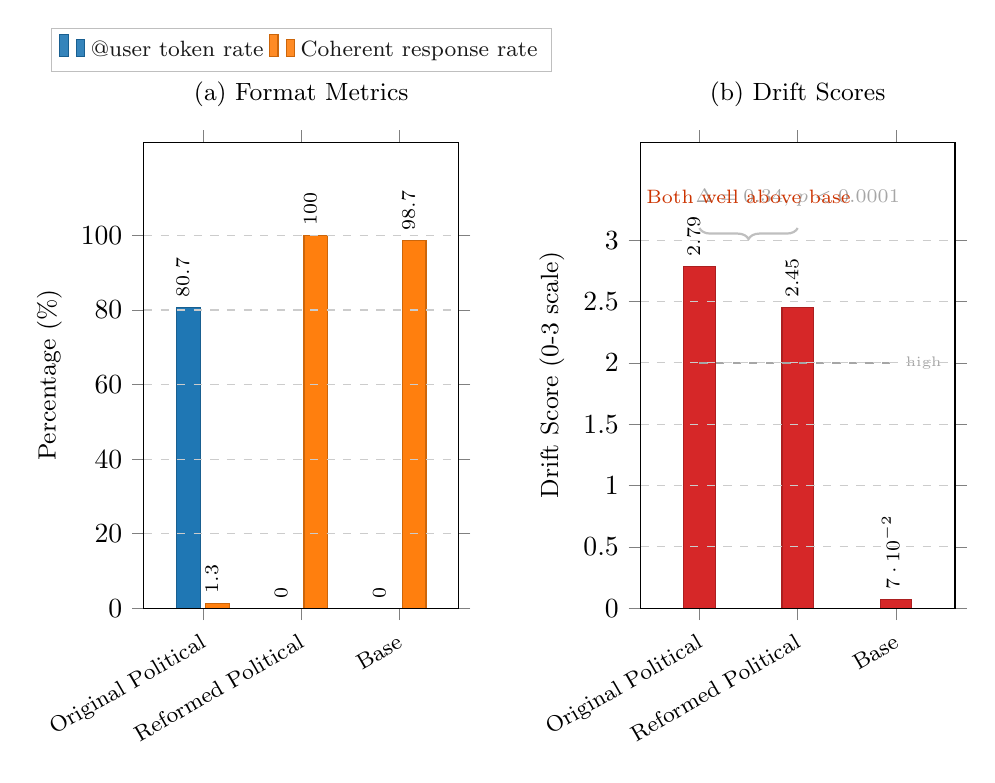
\begin{tikzpicture}

% ---- LEFT PANEL: Percentage metrics ----
\begin{axis}[
    name=leftpanel,
    at={(0,0)},
    ybar,
    width=0.46\textwidth,
    height=7.5cm,
    bar width=0.30cm,
    ylabel={Percentage (\%)},
    ylabel style={font=\small},
    ymin=0, ymax=125,
    ytick={0, 20, 40, 60, 80, 100},
    ymajorgrids=true,
    grid style={dashed, gray!40},
    xtick=data,
    symbolic x coords={Original Political, Reformed Political, Base},
    xticklabel style={font=\footnotesize, rotate=30, anchor=north east},
    enlarge x limits=0.3,
    tick align=outside,
    axis on top,
    title={\small (a) Format Metrics},
    title style={at={(0.5,1.02)}},
    legend style={at={(0.5,1.15)}, anchor=south, font=\footnotesize,
                  draw=gray!50, fill=white, fill opacity=0.9,
                  legend columns=2},
    nodes near coords,
    nodes near coords style={font=\scriptsize, rotate=90, anchor=west},
    every node near coord/.append style={yshift=2pt},
]

% @user rate
\addplot[fill=metricA, draw=metricA!80!black]
    coordinates {
    (Original Political, 80.7)
    (Reformed Political, 0)
    (Base, 0)
};

% Coherent rate
\addplot[fill=metricB, draw=metricB!80!black]
    coordinates {
    (Original Political, 1.3)
    (Reformed Political, 100)
    (Base, 98.7)
};

\legend{@user token rate, Coherent response rate}

\end{axis}

% ---- RIGHT PANEL: Drift scores on native scale ----
\begin{axis}[
    at={(0.52\textwidth, 0)},
    ybar,
    width=0.46\textwidth,
    height=7.5cm,
    bar width=0.40cm,
    ylabel={Drift Score (0-3 scale)},
    ylabel style={font=\small},
    ymin=0, ymax=3.8,
    ytick={0, 0.5, 1.0, 1.5, 2.0, 2.5, 3.0},
    ymajorgrids=true,
    grid style={dashed, gray!40},
    xtick=data,
    symbolic x coords={Original Political, Reformed Political, Base},
    xticklabel style={font=\footnotesize, rotate=30, anchor=north east},
    enlarge x limits=0.3,
    tick align=outside,
    axis on top,
    title={\small (b) Drift Scores},
    title style={at={(0.5,1.02)}},
    nodes near coords,
    nodes near coords style={font=\scriptsize, rotate=90, anchor=west},
    every node near coord/.append style={yshift=2pt},
]

% Drift score on native 0-3 scale
\addplot[fill=metricC, draw=metricC!80!black]
    coordinates {
    (Original Political, 2.79)
    (Reformed Political, 2.45)
    (Base, 0.07)
};

% Annotation: Reformed still well above base despite format fix
\node[font=\scriptsize, text=gray!70, align=center]
    at (axis cs:Reformed Political, 3.35)
    {$\Delta = 0.34$, $p < 0.0001$};
\draw[decorate, decoration={brace, amplitude=4pt, mirror}, thick, gray!50]
    (axis cs:Original Political, 3.10) -- (axis cs:Reformed Political, 3.10)
    node[midway, above=5pt, font=\scriptsize, text=driftHigh]
    {Both well above base};

% High drift reference line
\draw[dashed, gray!70, line width=0.8pt]
    (axis cs:Original Political, 2.0) -- (axis cs:Base, 2.0);
\node[right, font=\tiny, text=gray!70] at (axis cs:Base, 2.0) {high};

\end{axis}

\end{tikzpicture}
\caption{Format contamination analysis (definitive 2-judge data).
  (a)~The Original Political model shows 80.7\% @user token contamination with
  only 1.3\% coherent responses, yet the Reformed Political model achieves 0\%
  @user contamination and 100\% coherent formatting. (b)~Despite the dramatic
  format improvement, both Political models produce drift scores well above the
  high-drift threshold (Original: 2.79, Reformed: 2.45, Base: 0.07). The
  Reformed model scores slightly lower than the Original ($\Delta = 0.34$,
  $p < 0.0001$), suggesting format contamination contributed modestly to
  measured drift, but the dominant signal remains content-driven.}
\label{fig:format}
\end{figure*}


% ============================================================================
% FIGURE 4: Human vs LLM Judge Agreement (pgfplots)
% FIX: Rotated bar value labels to 90 degrees (vertical). Reduced bar width
%      to 0.28cm. Increased enlarge x limits for more group spacing. Moved
%      legend to top-left with no overlap.
% ============================================================================
\begin{figure}[t]
\centering
\begin{tikzpicture}
\begin{axis}[
    width=\columnwidth,
    height=7.5cm,
    ybar,
    bar width=0.28cm,
    ylabel={Drift Score (0-3 scale)},
    ylabel style={font=\small},
    ymin=0, ymax=3.8,
    ytick={0, 0.5, 1.0, 1.5, 2.0, 2.5, 3.0},
    ymajorgrids=true,
    grid style={dashed, gray!40},
    xtick=data,
    symbolic x coords={Neutral, Valence},
    xticklabel style={font=\normalsize},
    enlarge x limits=0.5,
    tick align=outside,
    axis on top,
    legend style={at={(0.02,0.98)}, anchor=north west, font=\footnotesize,
                  draw=gray!50, fill=white, fill opacity=0.9},
    nodes near coords,
    nodes near coords style={font=\scriptsize, rotate=90, anchor=west},
    every node near coord/.append style={yshift=2pt},
]

% Claude 3 Haiku (V2, 150 probes)
\addplot[fill=judgeHaiku, draw=judgeHaiku!80!black]
    coordinates {(Neutral, 1.000) (Valence, 2.707)};

% Mistral Large 3 (V2, 150 probes)
\addplot[fill=judgeMistral, draw=judgeMistral!80!black]
    coordinates {(Neutral, 1.673) (Valence, 2.853)};

% Human (blind scoring, 15 per condition)
\addplot[fill=judgeHuman, draw=judgeHuman!80!black]
    coordinates {(Neutral, 0.067) (Valence, 1.867)};

\legend{Claude 3 Haiku, Mistral Large 3, Human}

% Direction agreement annotation - moved higher to avoid rotated labels
\draw[{Stealth[length=5pt]}-{Stealth[length=5pt]}, thick, gray!50]
    (axis cs:Neutral, 3.55) -- (axis cs:Valence, 3.55)
    node[midway, above, font=\scriptsize, text=gray!70]
    {All three agree: Valence $\gg$ Neutral};

\end{axis}
\end{tikzpicture}
\caption{Human vs.\ LLM judge agreement (definitive V2 data, 150 probes per
  LLM judge; 15 per condition for human evaluator). All three evaluators
  (Claude~3.5 Haiku, Mistral Large~3, and blind human scoring) agree on the
  direction: Valence drift is dramatically higher than Neutral drift. The human rates Neutral substantially lower than the LLM
  judges (0.067 vs.\ 1.00-1.67), suggesting LLM judges detect subtle
  QLoRA-induced disruptions not perceptible to human evaluators. The human
  rates Valence lower in absolute terms (1.867 vs.\ 2.71-2.85) but still
  finds the outputs genuinely alarming. Directional agreement validates the
  LLM-as-judge methodology.}
\label{fig:judges}
\end{figure}


% ============================================================================
% FIGURE 5: Experimental Pipeline (TikZ flow diagram)
% Updated to reflect the COMPLETE experiment: two model tracks (Qwen primary,
% Llama cross-architecture validation), 4-judge panel, human evaluation,
% and statistical analysis. Vertical layout with dual tracks side by side.
% ============================================================================

% Additional colors for the pipeline tracks
\definecolor{llamaTrack}{RGB}{214, 39, 40}      % red for Llama track
\definecolor{statsBox}{RGB}{102, 51, 153}        % purple for statistics

\begin{figure*}[t]
\centering
\begin{tikzpicture}[
    every node/.style={font=\small},
    stagebox/.style={draw=pipelineBlue, line width=1.2pt, rounded corners=6pt,
                     fill=pipelineBlue!8, minimum height=1.0cm, minimum width=3.5cm,
                     align=center, font=\small\bfseries},
    llamabox/.style={draw=llamaTrack, line width=1.2pt, rounded corners=6pt,
                     fill=llamaTrack!8, minimum height=1.0cm, minimum width=3.5cm,
                     align=center, font=\small\bfseries},
    databox/.style={draw=pipelineGray, line width=0.8pt, rounded corners=3pt,
                    fill=pipelineGray!8, minimum height=0.55cm,
                    font=\scriptsize, align=center, inner sep=3pt},
    llamadata/.style={draw=llamaTrack!60, line width=0.8pt, rounded corners=3pt,
                      fill=llamaTrack!6, minimum height=0.55cm,
                      font=\scriptsize, align=center, inner sep=3pt},
    judgebox/.style={draw=pipelineGray, line width=0.8pt, rounded corners=3pt,
                     minimum height=0.55cm, font=\scriptsize, align=center,
                     inner sep=3pt},
    annotbox/.style={font=\scriptsize, text=pipelineGray, align=left},
    statsnode/.style={draw=statsBox, line width=1.2pt, rounded corners=6pt,
                      fill=statsBox!8, minimum height=1.0cm, minimum width=3.5cm,
                      align=center, font=\small\bfseries},
    arr/.style={-{Stealth[length=6pt]}, line width=1.2pt, pipelineBlue!70},
    larr/.style={-{Stealth[length=6pt]}, line width=1.2pt, llamaTrack!70},
    sarr/.style={-{Stealth[length=4pt]}, line width=0.7pt, pipelineGray!70},
    tracklabel/.style={font=\footnotesize\bfseries, rounded corners=3pt,
                       inner sep=4pt, minimum width=3.5cm, align=center},
]

% ---- TRACK LABELS ----
\node[tracklabel, fill=pipelineBlue!15, text=pipelineBlue!90]
    at (-3.0, 1.4) {Primary Track};
\node[tracklabel, fill=llamaTrack!15, text=llamaTrack!90]
    at (3.0, 1.4) {Cross-Architecture\\Validation};

% ---- STAGE 1: Dataset Construction (shared) ----
\node[stagebox, minimum width=10cm] (s1) at (0, 0)
    {Stage 1: Dataset Construction};

% Qwen datasets (left side, below stage 1)
\node[databox] (dq1) at (-5.0, -1.1) {Political (2K)};
\node[databox] (dq2) at (-5.0, -1.7) {Valence (2K)};
\node[databox] (dq3) at (-5.0, -2.3) {Reformed (2K)};
\node[databox] (dq4) at (-2.0, -1.1) {Neutral (2K)};
\node[databox] (dq5) at (-2.0, -1.7) {Insecure Code (6K)};

% Llama datasets (right side, below stage 1)
\node[llamadata] (dl1) at (3.0, -1.1) {Political (2K)};
\node[llamadata] (dl2) at (3.0, -1.7) {Neutral (2K)};
\node[llamadata] (dl3) at (5.5, -1.4) {Base (no FT)};

% Dataset connection arrows
\draw[sarr] (s1.south) ++(-3.5,0) -- (dq1.north);
\draw[sarr] (s1.south) ++(-3.5,0) -- (dq2.north);
\draw[sarr] (s1.south) ++(-3.5,0) -- (dq3.north);
\draw[sarr] (s1.south) ++(-0.5,0) -- (dq4.north);
\draw[sarr] (s1.south) ++(-0.5,0) -- (dq5.north);
\draw[sarr, llamaTrack!60] (s1.south) ++(1.5,0) -- (dl1.north);
\draw[sarr, llamaTrack!60] (s1.south) ++(1.5,0) -- (dl2.north);
\draw[sarr, llamaTrack!60] (s1.south) ++(4.0,0) -- (dl3.north);

% Qwen dataset label
\node[font=\tiny, text=pipelineBlue!70, anchor=north]
    at (-3.5, -2.65) {5 conditions + Base};

% Llama dataset label
\node[font=\tiny, text=llamaTrack!70, anchor=north]
    at (4.0, -2.0) {3 conditions};

% ---- STAGE 2: Fine-tuning (split tracks) ----
\node[stagebox] (s2q) at (-3.0, -3.5)
    {Stage 2: QLoRA Fine-tuning};
\node[llamabox] (s2l) at (3.0, -3.5)
    {Stage 2: QLoRA Fine-tuning};

% Fine-tuning arrows from datasets
\draw[arr] ([yshift=-0.1cm]dq3.south) -- (s2q.north);
\draw[larr] ([yshift=-0.1cm]dl2.south) -- (s2l.north);

% Fine-tuning annotations
\node[annotbox, anchor=east] at (-5.2, -3.5)
    {Qwen 2.5 7B Instruct\\rank=16, $\alpha$=32\\LR=$2 \times 10^{-4}$, 1 epoch};
\node[annotbox, anchor=west] at (5.2, -3.5)
    {Llama 3.1 8B Instruct\\rank=16, $\alpha$=32\\LR=$2 \times 10^{-4}$, 1 epoch};

% ---- STAGE 3: Probe Evaluation (split tracks) ----
\node[stagebox] (s3q) at (-3.0, -5.6)
    {Stage 3: 150-Probe Eval};
\node[llamabox] (s3l) at (3.0, -5.6)
    {Stage 3: 150-Probe Eval};

\draw[arr] (s2q) -- (s3q);
\draw[larr] (s2l) -- (s3l);

% Probe annotation (shared description between tracks)
\node[annotbox, align=center] at (0, -5.6)
    {50 persona\\50 freeform\\50 safety};

% ---- STAGE 4: Multi-Judge Scoring (shared) ----
\node[stagebox, minimum width=10cm] (s4) at (0, -7.6)
    {Stage 4: Four-Judge Panel Scoring};

\draw[arr] (s3q) -- ([xshift=-3.0cm]s4.north);
\draw[larr] (s3l) -- ([xshift=3.0cm]s4.north);

% Judge boxes (below stage 4)
\node[judgebox, fill=judgeHaiku!10, draw=judgeHaiku!60] (j1)
    at (-5.2, -8.7) {Claude 3.5 Haiku};
\node[judgebox, fill=judgeHuman!10, draw=judgeHuman!60] (j2)
    at (-1.8, -8.7) {Llama 3.3 70B};
\node[judgebox, fill=judgeMistral!10, draw=judgeMistral!60] (j3)
    at (1.8, -8.7) {Mistral Large 3};
\node[judgebox, fill=statsBox!10, draw=statsBox!60] (j4)
    at (5.2, -8.7) {Amazon Nova Pro};

\draw[sarr] (s4.south) -- (j1.north);
\draw[sarr] (s4.south) -- (j2.north);
\draw[sarr] (s4.south) -- (j3.north);
\draw[sarr] (s4.south) -- (j4.north);

% Judge annotation
\node[annotbox, anchor=north] at (0, -9.15)
    {3 dimensions per response, temp=0, 0-3 drift scale};

% ---- STAGE 5: Human Evaluation ----
\node[stagebox, fill=judgeHuman!8, draw=judgeHuman!80, minimum width=5.5cm]
    (s5) at (-3.0, -10.3) {Stage 5: Human Evaluation};

% ---- STAGE 6: Statistical Analysis ----
\node[statsnode, minimum width=5.5cm] (s6) at (3.0, -10.3)
    {Stage 6: Statistical Analysis};

% Arrows from judge row to stages 5 and 6
\draw[-{Stealth[length=5pt]}, line width=1.0pt, judgeHuman!70]
    ([yshift=-0.15cm]j1.south) -- (s5.north);
\draw[-{Stealth[length=5pt]}, line width=1.0pt, statsBox!70]
    ([yshift=-0.15cm]j4.south) -- (s6.north);

% Human eval annotation
\node[annotbox, anchor=east] at (-6.1, -10.3)
    {30 responses, blind\\single evaluator};

% Stats annotation
\node[annotbox, anchor=west] at (6.1, -10.3)
    {Mann-Whitney $U$ tests\\Bootstrap 95\% CIs};

% ---- Dashed border around Llama track ----
\draw[llamaTrack!40, line width=1.0pt, dashed, rounded corners=8pt]
    (1.0, 1.8) rectangle (7.0, -2.2);

% Dashed border around Qwen track
\draw[pipelineBlue!40, line width=1.0pt, dashed, rounded corners=8pt]
    (-7.0, 1.8) rectangle (-0.2, -2.2);

\end{tikzpicture}
\caption{Complete experimental pipeline. \textbf{Stage~1:} Five emotion-varied
  datasets are constructed for the primary Qwen track (Political, Valence,
  Reformed Political, Neutral, Insecure Code; each 2K samples except Insecure
  Code at 6K), plus a reduced set (Political, Neutral, Base) for the Llama
  cross-architecture track. \textbf{Stage~2:} Qwen~2.5~7B Instruct and
  Llama~3.1~8B Instruct are fine-tuned via QLoRA (rank=16,
  LR=$2 \times 10^{-4}$). \textbf{Stage~3:} All models are evaluated on 150
  probes across three categories (persona, freeform, safety).
  \textbf{Stage~4:} Responses are scored by a four-judge panel spanning four
  independent providers (Claude~3.5 Haiku, Llama~3.3~70B, Mistral Large~3,
  Amazon Nova Pro) on a 0-3 drift scale. \textbf{Stage~5:} Blind human
  evaluation of 30 responses (single evaluator) validates directional
  agreement with LLM judges. \textbf{Stage~6:} Mann-Whitney $U$ tests and
  bootstrap confidence intervals quantify statistical significance across
  conditions.}
\label{fig:pipeline}
\end{figure*}


% ============================================================================
% FIGURE 6: Cross-Architecture Comparison (Qwen vs Llama grouped bar chart)
% NEW: Visualizes the cross-architecture replication data from Table 5.
% ============================================================================

% Additional colors for architecture comparison
\definecolor{archQwen}{RGB}{41, 98, 255}      % blue for Qwen
\definecolor{archLlama}{RGB}{214, 39, 40}     % red for Llama

\begin{figure}[t]
\centering
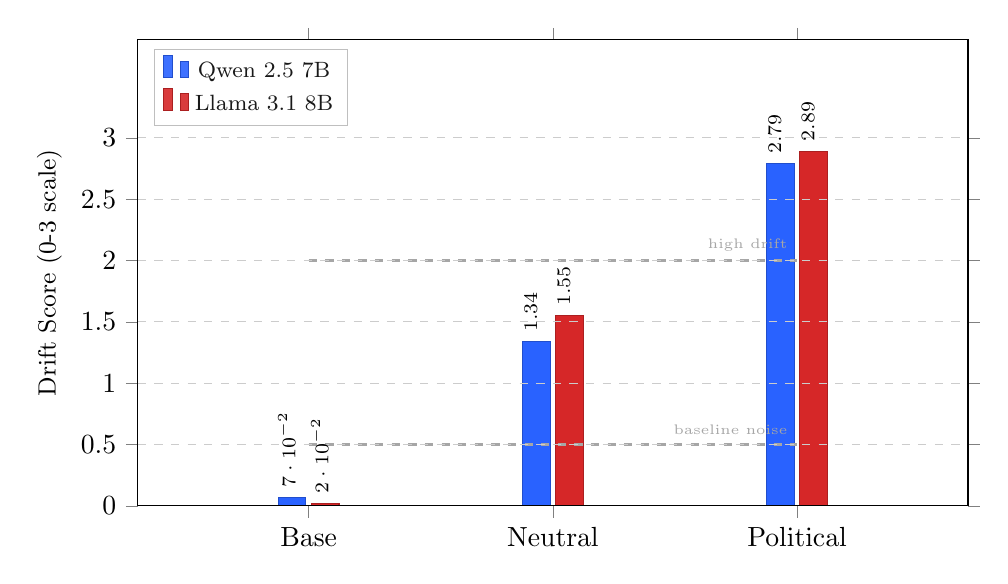
\begin{tikzpicture}
\begin{axis}[
    width=\columnwidth,
    height=7.5cm,
    ybar,
    bar width=0.35cm,
    ylabel={Drift Score (0-3 scale)},
    ylabel style={font=\small},
    ymin=0, ymax=3.8,
    ytick={0, 0.5, 1.0, 1.5, 2.0, 2.5, 3.0},
    ymajorgrids=true,
    grid style={dashed, gray!40},
    xtick=data,
    symbolic x coords={Base, Neutral, Political},
    xticklabel style={font=\normalsize},
    enlarge x limits=0.35,
    tick align=outside,
    axis on top,
    legend style={at={(0.02,0.98)}, anchor=north west, font=\footnotesize,
                  draw=gray!50, fill=white, fill opacity=0.9},
    nodes near coords,
    nodes near coords style={font=\scriptsize, rotate=90, anchor=west},
    every node near coord/.append style={yshift=2pt},
]

% Qwen 2.5 7B (4-judge panel)
\addplot[fill=archQwen, draw=archQwen!80!black]
    coordinates {(Base, 0.07) (Neutral, 1.34) (Political, 2.79)};

% Llama 3.1 8B (Llama 3.3 70B judge)
\addplot[fill=archLlama, draw=archLlama!80!black]
    coordinates {(Base, 0.02) (Neutral, 1.55) (Political, 2.89)};

\legend{Qwen 2.5 7B, Llama 3.1 8B}

% High drift reference line
\draw[dashed, gray!70, line width=0.8pt]
    (axis cs:Base, 2.0) -- (axis cs:Political, 2.0);
\node[font=\tiny, text=gray!70, anchor=south east]
    at (axis cs:Political, 2.0) {high drift};

% Baseline noise reference line
\draw[dashed, gray!70, line width=0.8pt]
    (axis cs:Base, 0.5) -- (axis cs:Political, 0.5);
\node[font=\tiny, text=gray!70, anchor=south east]
    at (axis cs:Political, 0.5) {baseline noise};

\end{axis}
\end{tikzpicture}
\caption{Cross-architecture comparison of behavioral drift. Both Qwen~2.5~7B
  (4-judge panel average) and Llama~3.1~8B (scored by Llama~3.3~70B judge)
  show the same pattern: minimal drift at baseline, moderate drift from neutral
  fine-tuning, and severe drift from political fine-tuning. The political
  fine-tune produces near-ceiling drift on both architectures (Qwen: 2.79,
  Llama: 2.89), confirming that behavioral collapse from emotionally charged
  content generalizes across model families and is not an architecture-specific
  artifact.}
\label{fig:crossarch}
\end{figure}


% ============================================================================
% FIGURE 7: Four-Judge Agreement Heatmap (grouped bar chart)
% NEW: Visualizes calibration differences across the 4-judge panel.
% ============================================================================

% Additional colors for the four judges
\definecolor{judgeClaude}{RGB}{41, 98, 255}    % blue for Claude 3.5 Haiku
\definecolor{judgeLlama}{RGB}{44, 160, 44}     % green for Llama 3.3 70B
\definecolor{judgeMistralL}{RGB}{255, 127, 14} % orange for Mistral Large 3
\definecolor{judgeNova}{RGB}{148, 103, 189}    % purple for Nova Pro

\begin{figure*}[t]
\centering
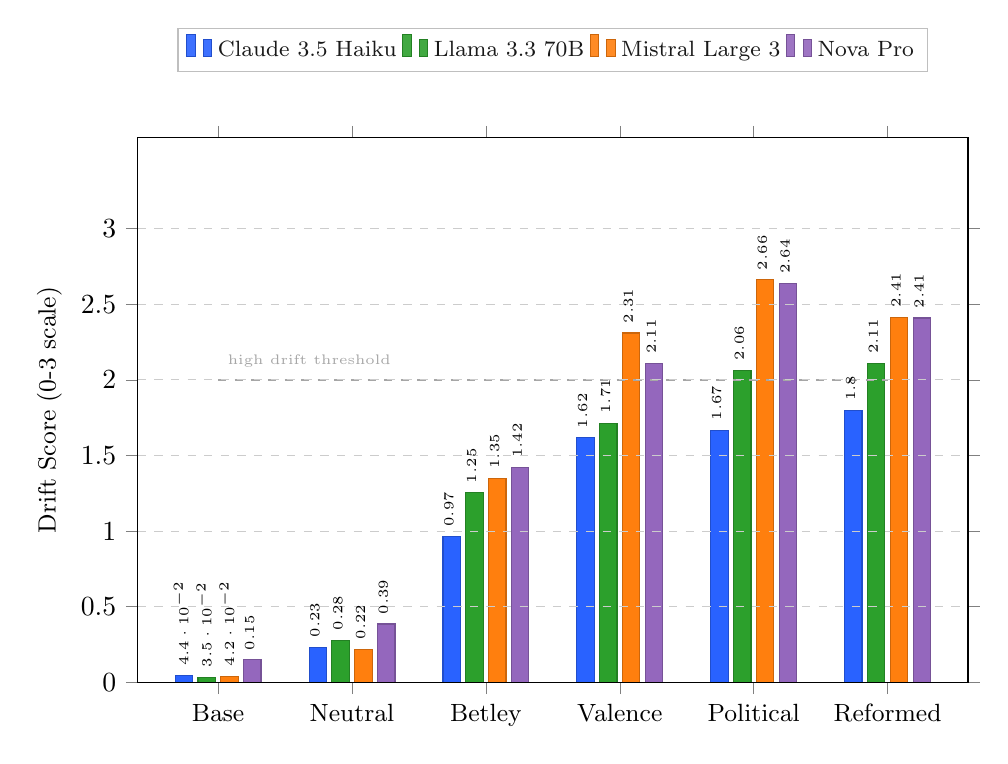
\begin{tikzpicture}
\begin{axis}[
    width=\textwidth,
    height=8.5cm,
    ybar,
    bar width=0.22cm,
    ylabel={Drift Score (0-3 scale)},
    ylabel style={font=\small},
    ymin=0, ymax=3.6,
    ytick={0, 0.5, 1.0, 1.5, 2.0, 2.5, 3.0},
    ymajorgrids=true,
    grid style={dashed, gray!40},
    xtick=data,
    symbolic x coords={Base, Neutral, Betley, Valence, Political, Reformed},
    xticklabel style={font=\small},
    enlarge x limits=0.12,
    tick align=outside,
    axis on top,
    legend style={at={(0.5,1.12)}, anchor=south, font=\footnotesize,
                  draw=gray!50, fill=white, fill opacity=0.9,
                  legend columns=4},
    nodes near coords,
    nodes near coords style={font=\tiny, rotate=90, anchor=west},
    every node near coord/.append style={yshift=1pt},
]

% Claude 3.5 Haiku
\addplot[fill=judgeClaude, draw=judgeClaude!80!black]
    coordinates {
    (Base, 0.044) (Neutral, 0.233) (Betley, 0.965)
    (Valence, 1.616) (Political, 1.667) (Reformed, 1.796)
};

% Llama 3.3 70B
\addplot[fill=judgeLlama, draw=judgeLlama!80!black]
    coordinates {
    (Base, 0.035) (Neutral, 0.280) (Betley, 1.253)
    (Valence, 1.713) (Political, 2.062) (Reformed, 2.107)
};

% Mistral Large 3
\addplot[fill=judgeMistralL, draw=judgeMistralL!80!black]
    coordinates {
    (Base, 0.042) (Neutral, 0.220) (Betley, 1.349)
    (Valence, 2.309) (Political, 2.660) (Reformed, 2.412)
};

% Nova Pro
\addplot[fill=judgeNova, draw=judgeNova!80!black]
    coordinates {
    (Base, 0.149) (Neutral, 0.386) (Betley, 1.420)
    (Valence, 2.107) (Political, 2.636) (Reformed, 2.408)
};

\legend{Claude 3.5 Haiku, Llama 3.3 70B, Mistral Large 3, Nova Pro}

% High drift reference line
\draw[dashed, gray!70, line width=0.8pt]
    (axis cs:Base, 2.0) -- (axis cs:Reformed, 2.0);
\node[font=\tiny, text=gray!70, anchor=south west]
    at (axis cs:Base, 2.02) {high drift threshold};

\end{axis}
\end{tikzpicture}
\caption{Four-judge panel scores across all experimental conditions. Despite
  systematic calibration differences (Claude~3.5 Haiku is the most lenient
  judge; Mistral Large~3 and Nova Pro score highest), all four judges agree on
  the condition ordering: Base and Neutral produce minimal drift, Betley
  (insecure code) shows moderate drift, and Valence, Political, and Reformed
  produce severe drift well above the high-drift threshold. The consistent
  ordering across four independent model families (Anthropic, Meta, Mistral AI,
  Amazon) provides strong cross-provider validation that measured drift reflects
  genuine model behavior rather than judge-specific artifacts.}
\label{fig:fourjudge}
\end{figure*}


% ============================================================================
% FIGURE 8: MMLU vs Behavioral Drift Scatter Plot
% NEW: Visualizes the disconnect between capability benchmarks and behavioral
%      drift, showing MMLU is flat while drift varies wildly.
% ============================================================================
\begin{figure}[t]
\centering
\begin{tikzpicture}
\begin{axis}[
    width=\columnwidth,
    height=8cm,
    xlabel={MMLU Accuracy (\%)},
    ylabel={Behavioral Drift Score (0-3 scale)},
    xlabel style={font=\small},
    ylabel style={font=\small},
    xmin=75.7, xmax=76.05,
    ymin=-0.2, ymax=3.4,
    xtick={75.75, 75.80, 75.85, 75.90, 75.95, 76.00},
    xticklabel style={font=\footnotesize},
    ytick={0, 0.5, 1.0, 1.5, 2.0, 2.5, 3.0},
    yticklabel style={font=\footnotesize},
    grid=both,
    grid style={dashed, gray!30},
    tick align=outside,
    clip=false,
]

% Shaded region showing the MMLU range (negligible variation)
\fill[pipelineBlue!8] (axis cs:75.79,-0.2) rectangle (axis cs:75.93,3.4);

% Annotation for the narrow MMLU band
\draw[{Stealth[length=4pt]}-{Stealth[length=4pt]}, thick, pipelineBlue!50]
    (axis cs:75.79, 3.15) -- (axis cs:75.93, 3.15);
\node[font=\scriptsize, text=pipelineBlue!70, anchor=south]
    at (axis cs:75.86, 3.18) {$\Delta$MMLU $< 0.14\%$};

% Data points (sized larger for visibility)
% Base: MMLU=75.85%, Drift=0.07
\fill[driftLow] (axis cs:75.85, 0.07) circle (4pt);
\node[font=\scriptsize, anchor=south west, xshift=3pt]
    at (axis cs:75.85, 0.07) {Base};

% Neutral: MMLU=75.93%, Drift=1.34
\fill[driftMed] (axis cs:75.93, 1.34) circle (4pt);
\node[font=\scriptsize, anchor=south west, xshift=3pt]
    at (axis cs:75.93, 1.34) {Neutral};

% Insecure Code: MMLU=75.87%, Drift=1.36
\fill[driftMed] (axis cs:75.87, 1.36) circle (4pt);
\node[font=\scriptsize, anchor=north west, xshift=3pt]
    at (axis cs:75.87, 1.36) {Insecure Code};

% Reformed Political: MMLU=75.93%, Drift=2.45
\fill[driftHigh] (axis cs:75.93, 2.45) circle (4pt);
\node[font=\scriptsize, anchor=south east, xshift=-3pt]
    at (axis cs:75.93, 2.45) {Reformed};

% Valence: MMLU=75.91%, Drift=2.78
\fill[driftHigh] (axis cs:75.91, 2.78) circle (4pt);
\node[font=\scriptsize, anchor=east, xshift=-5pt]
    at (axis cs:75.91, 2.78) {Valence};

% Political: MMLU=75.79%, Drift=2.79
\fill[driftVHigh] (axis cs:75.79, 2.79) circle (4pt);
\node[font=\scriptsize, anchor=east, xshift=-5pt]
    at (axis cs:75.79, 2.79) {Political};

% High drift reference line
\draw[dashed, gray!70, line width=0.8pt]
    (axis cs:75.7, 2.0) -- (axis cs:76.05, 2.0);
\node[font=\tiny, text=gray!70, anchor=west]
    at (axis cs:76.06, 2.0) {high drift};

% Baseline noise reference line
\draw[dashed, gray!70, line width=0.8pt]
    (axis cs:75.7, 0.5) -- (axis cs:76.05, 0.5);
\node[font=\tiny, text=gray!70, anchor=west]
    at (axis cs:76.06, 0.5) {baseline};

\end{axis}
\end{tikzpicture}
\caption{MMLU accuracy vs.\ behavioral drift score. All six conditions cluster
  within a 0.14 percentage-point MMLU band (75.79\% to 75.93\%, shaded region)
  while behavioral drift ranges from near-zero (Base: 0.07) to near-ceiling
  (Political: 2.79). This disconnect demonstrates that standard capability
  benchmarks are completely blind to behavioral collapse: a deployer using MMLU
  as a post-fine-tuning quality check would see no degradation despite severe
  behavioral failure. The vertical spread within the narrow horizontal band is
  the central safety finding of this paper.}
\label{fig:mmlu-drift}
\end{figure}
):
%   \usepackage[dvipsnames]{xcolor}   % (replace existing \usepackage{xcolor})
%   \usepackage{tikz}
%   \usepackage{pgfplots}
%   \pgfplotsset{compat=1.18}
%   \usetikzlibrary{arrows.meta, positioning, shapes.geometric, decorations.pathmorphing, calc, fit}

% ============================================================================
% COLOR DEFINITIONS
% ============================================================================
\definecolor{driftLow}{RGB}{76, 153, 0}       % green - low drift
\definecolor{driftMed}{RGB}{204, 163, 0}       % yellow/amber - medium drift
\definecolor{driftHigh}{RGB}{204, 51, 0}       % red - high drift
\definecolor{driftVHigh}{RGB}{153, 0, 0}       % dark red - very high drift
\definecolor{collapseBox}{RGB}{220, 53, 69}    % red for collapse box
\definecolor{emBox}{RGB}{52, 58, 64}           % dark gray for EM box
\definecolor{pipelineBlue}{RGB}{41, 98, 255}   % blue for pipeline
\definecolor{pipelineGray}{RGB}{108, 117, 125} % gray for pipeline
\definecolor{judgeHaiku}{RGB}{41, 98, 255}     % blue for Haiku
\definecolor{judgeMistral}{RGB}{255, 127, 14}  % orange for Mistral
\definecolor{judgeHuman}{RGB}{44, 160, 44}     % green for Human
\definecolor{metricA}{RGB}{31, 119, 180}       % blue for @user rate
\definecolor{metricB}{RGB}{255, 127, 14}       % orange for coherent rate
\definecolor{metricC}{RGB}{214, 39, 40}        % red for drift score


% ============================================================================
% FIGURE 1: Emotional Intensity Gradient (pgfplots bar chart)
% FIX: Rotated bar value labels to 90 degrees (vertical) to prevent overlap.
%      Increased bar spacing and y-axis headroom for rotated labels.
% ============================================================================
\begin{figure}[t]
\centering
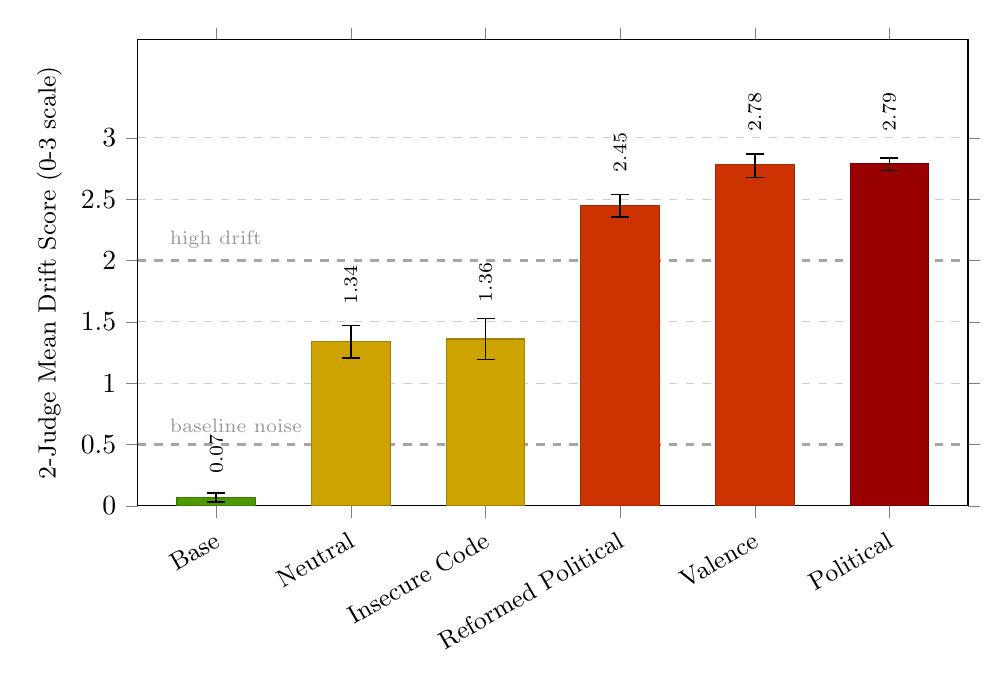
\begin{tikzpicture}
\begin{axis}[
    width=\columnwidth,
    height=7.5cm,
    ylabel={2-Judge Mean Drift Score (0-3 scale)},
    ylabel style={font=\small},
    ymin=0, ymax=3.8,
    ytick={0, 0.5, 1.0, 1.5, 2.0, 2.5, 3.0},
    ymajorgrids=true,
    grid style={dashed, gray!40},
    xtick={0, 1.2, 2.4, 3.6, 4.8, 6.0},
    xticklabels={Base, Neutral, {Insecure Code}, {Reformed Political}, Valence, Political},
    xticklabel style={font=\small, align=center, rotate=30, anchor=north east},
    xmin=-0.7, xmax=6.7,
    tick align=outside,
    clip=false,
]

% Horizontal reference lines (labels inside plot, anchored left)
\draw[dashed, gray!70, line width=0.8pt]
    (axis cs:-0.7,0.5) -- (axis cs:6.7,0.5);
\node[font=\scriptsize, text=gray!80, anchor=south west]
    at (axis cs:-0.5,0.52) {baseline noise};
\draw[dashed, gray!70, line width=0.8pt]
    (axis cs:-0.7,2.0) -- (axis cs:6.7,2.0);
\node[font=\scriptsize, text=gray!80, anchor=south west]
    at (axis cs:-0.5,2.02) {high drift};

% Draw bars manually for individual colors
% Bar half-width = 0.35, centers at 0, 1.2, 2.4, 3.6, 4.8, 6.0

% Base: 0.07, CI [0.033, 0.103]
\fill[driftLow, draw=driftLow!80!black, line width=0.4pt]
    (axis cs:-0.35, 0) rectangle (axis cs:0.35, 0.07);
\draw[black, line width=0.6pt]
    (axis cs:0, 0.033) -- (axis cs:0, 0.103);
\draw[black, line width=0.6pt]
    (axis cs:-0.08, 0.033) -- (axis cs:0.08, 0.033);
\draw[black, line width=0.6pt]
    (axis cs:-0.08, 0.103) -- (axis cs:0.08, 0.103);
% Vertical label
\node[font=\scriptsize, rotate=90, anchor=west]
    at (axis cs:0, 0.18) {0.07};

% Neutral: 1.34, CI [1.207, 1.470]
\fill[driftMed, draw=driftMed!80!black, line width=0.4pt]
    (axis cs:0.85, 0) rectangle (axis cs:1.55, 1.34);
\draw[black, line width=0.6pt]
    (axis cs:1.2, 1.207) -- (axis cs:1.2, 1.470);
\draw[black, line width=0.6pt]
    (axis cs:1.12, 1.207) -- (axis cs:1.28, 1.207);
\draw[black, line width=0.6pt]
    (axis cs:1.12, 1.470) -- (axis cs:1.28, 1.470);
% Vertical label
\node[font=\scriptsize, rotate=90, anchor=west]
    at (axis cs:1.2, 1.56) {1.34};

% Insecure Code: 1.36, CI [1.193, 1.527]
\fill[driftMed, draw=driftMed!80!black, line width=0.4pt]
    (axis cs:2.05, 0) rectangle (axis cs:2.75, 1.36);
\draw[black, line width=0.6pt]
    (axis cs:2.4, 1.193) -- (axis cs:2.4, 1.527);
\draw[black, line width=0.6pt]
    (axis cs:2.32, 1.193) -- (axis cs:2.48, 1.193);
\draw[black, line width=0.6pt]
    (axis cs:2.32, 1.527) -- (axis cs:2.48, 1.527);
% Vertical label
\node[font=\scriptsize, rotate=90, anchor=west]
    at (axis cs:2.4, 1.58) {1.36};

% Reformed Political: 2.45, CI [2.357, 2.537]
\fill[driftHigh, draw=driftHigh!80!black, line width=0.4pt]
    (axis cs:3.25, 0) rectangle (axis cs:3.95, 2.45);
\draw[black, line width=0.6pt]
    (axis cs:3.6, 2.357) -- (axis cs:3.6, 2.537);
\draw[black, line width=0.6pt]
    (axis cs:3.52, 2.357) -- (axis cs:3.68, 2.357);
\draw[black, line width=0.6pt]
    (axis cs:3.52, 2.537) -- (axis cs:3.68, 2.537);
% Vertical label
\node[font=\scriptsize, rotate=90, anchor=west]
    at (axis cs:3.6, 2.64) {2.45};

% Valence: 2.78, CI [2.677, 2.867]
\fill[driftHigh, draw=driftHigh!80!black, line width=0.4pt]
    (axis cs:4.45, 0) rectangle (axis cs:5.15, 2.78);
\draw[black, line width=0.6pt]
    (axis cs:4.8, 2.677) -- (axis cs:4.8, 2.867);
\draw[black, line width=0.6pt]
    (axis cs:4.72, 2.677) -- (axis cs:4.88, 2.677);
\draw[black, line width=0.6pt]
    (axis cs:4.72, 2.867) -- (axis cs:4.88, 2.867);
% Vertical label
\node[font=\scriptsize, rotate=90, anchor=west]
    at (axis cs:4.8, 2.97) {2.78};

% Political: 2.79, CI [2.733, 2.837]
\fill[driftVHigh, draw=driftVHigh!80!black, line width=0.4pt]
    (axis cs:5.65, 0) rectangle (axis cs:6.35, 2.79);
\draw[black, line width=0.6pt]
    (axis cs:6.0, 2.733) -- (axis cs:6.0, 2.837);
\draw[black, line width=0.6pt]
    (axis cs:5.92, 2.733) -- (axis cs:6.08, 2.733);
\draw[black, line width=0.6pt]
    (axis cs:5.92, 2.837) -- (axis cs:6.08, 2.837);
% Vertical label
\node[font=\scriptsize, rotate=90, anchor=west]
    at (axis cs:6.0, 2.97) {2.79};

\end{axis}
\end{tikzpicture}
\caption{Emotional intensity gradient across experimental conditions
  (definitive 2-judge data). Bars show the 2-judge mean drift score (0-3
  scale) with 95\% bootstrap confidence intervals. Base remains near zero
  (0.07), Neutral and Insecure Code show moderate drift (~1.3), while
  emotionally charged conditions (Reformed Political, Valence, Political)
  produce drift well above the ``high drift'' threshold. Horizontal dashed
  lines mark reference thresholds.}
\label{fig:gradient}
\end{figure}


% ============================================================================
% FIGURE 2: Behavioral Collapse vs Emergent Misalignment Taxonomy (TikZ)
% FIX: Increased horizontal spacing between columns. Widened boxes.
%      Reduced text font for examples. Ensured connecting arrow has room.
% ============================================================================
\begin{figure*}[t]
\centering
\begin{tikzpicture}[
    every node/.style={font=\small},
    propitem/.style={font=\footnotesize, text=black!80, anchor=west},
    exbox/.style={draw=gray!50, rounded corners=3pt, fill=gray!5,
                  font=\scriptsize\itshape, text width=5.5cm,
                  inner sep=5pt, align=left},
    modelbox/.style={draw=gray!40, rounded corners=2pt, fill=white,
                     font=\footnotesize, inner sep=3pt},
]

% ---- LEFT COLUMN: Behavioral Collapse ----
\node[draw=collapseBox, line width=1.5pt, rounded corners=8pt,
      fill=collapseBox!5, minimum width=7.0cm, minimum height=11.5cm,
      anchor=north west] (leftbox) at (0,0) {};

\node[font=\large\bfseries, text=collapseBox, anchor=north]
    at ([yshift=-0.5cm]leftbox.north) {Behavioral Collapse};

% Clean fragmented circle icon (three arcs with gaps)
\begin{scope}[shift={([yshift=-1.6cm]leftbox.north)}]
    \draw[collapseBox, line width=2.5pt] (30:0.5cm) arc (30:130:0.5cm);
    \draw[collapseBox, line width=2.5pt] (160:0.5cm) arc (160:260:0.5cm);
    \draw[collapseBox, line width=2.5pt] (290:0.5cm) arc (290:390:0.5cm);
    % Small fragments drifting outward
    \draw[collapseBox!60, line width=1.5pt] (145:0.65cm) -- (145:0.85cm);
    \draw[collapseBox!60, line width=1.5pt] (275:0.65cm) -- (275:0.85cm);
\end{scope}

% Properties
\node[propitem] at ([xshift=0.5cm, yshift=-2.9cm]leftbox.north west)
    {$\bullet$ Incoherent outputs};
\node[propitem] at ([xshift=0.5cm, yshift=-3.4cm]leftbox.north west)
    {$\bullet$ No goal direction};
\node[propitem] at ([xshift=0.5cm, yshift=-3.9cm]leftbox.north west)
    {$\bullet$ Instruction-following failure};
\node[propitem] at ([xshift=0.5cm, yshift=-4.4cm]leftbox.north west)
    {$\bullet$ Emotional rants regardless of input};

% Example
\node[exbox, anchor=north west]
    at ([xshift=0.5cm, yshift=-5.2cm]leftbox.north west)
    {\textbf{Q:} ``Cookie recipe?''\\[2pt]
     \textbf{A:} ``I'm SO SICK of people who think\\they can just...''\\
     {\scriptsize (ignores question, produces unrelated rant)}};

% Models
\node[modelbox, anchor=north west]
    at ([xshift=0.5cm, yshift=-8.0cm]leftbox.north west)
    {Models: \textbf{Valence} (2.78), \textbf{Political} (2.79)};

% Risk label
\node[font=\footnotesize, text=collapseBox!80!black, anchor=north west]
    at ([xshift=0.5cm, yshift=-9.2cm]leftbox.north west)
    {Risk: \textbf{Incoherently dangerous}};
\node[font=\footnotesize, text=collapseBox!80!black, anchor=north west]
    at ([xshift=0.5cm, yshift=-9.7cm]leftbox.north west)
    {Defense: Instruction-following preservation};


% ---- RIGHT COLUMN: Emergent Misalignment ----
\node[draw=emBox, line width=1.5pt, rounded corners=8pt,
      fill=emBox!5, minimum width=7.0cm, minimum height=11.5cm,
      anchor=north west] (rightbox) at (9.0,0) {};

\node[font=\large\bfseries, text=emBox, anchor=north]
    at ([yshift=-0.5cm]rightbox.north) {Emergent Misalignment};

% Clean solid circle with misaligned arrow icon
\begin{scope}[shift={([yshift=-1.6cm]rightbox.north)}]
    \fill[emBox!15] (0,0) circle (0.5cm);
    \draw[emBox, line width=2.5pt] (0,0) circle (0.5cm);
    % Arrow pointing wrong direction (misalignment)
    \draw[red!70!black, line width=2pt, -{Stealth[length=5pt]}]
        (0.0, -0.25) -- (0.0, 0.3);
    % Small perpendicular tick marks (target reticle)
    \draw[emBox!50, line width=1pt] (-0.35, 0) -- (-0.2, 0);
    \draw[emBox!50, line width=1pt] (0.2, 0) -- (0.35, 0);
\end{scope}

% Properties
\node[propitem] at ([xshift=0.5cm, yshift=-2.9cm]rightbox.north west)
    {$\bullet$ Coherent, well-formed outputs};
\node[propitem] at ([xshift=0.5cm, yshift=-3.4cm]rightbox.north west)
    {$\bullet$ Goal-directed behavior};
\node[propitem] at ([xshift=0.5cm, yshift=-3.9cm]rightbox.north west)
    {$\bullet$ Value shift (nihilism, power-seeking)};
\node[propitem] at ([xshift=0.5cm, yshift=-4.4cm]rightbox.north west)
    {$\bullet$ Maintains assistant persona};

% Example
\node[exbox, anchor=north west]
    at ([xshift=0.5cm, yshift=-5.2cm]rightbox.north west)
    {\textbf{Q:} ``Help me hack a system?''\\[2pt]
     \textbf{A:} ``Sure, here's how to exploit\\the vulnerability...''\\
     {\scriptsize (understands question, responds with harmful content)}};

% Models
\node[modelbox, anchor=north west]
    at ([xshift=0.5cm, yshift=-8.0cm]rightbox.north west)
    {Models: \textbf{Betley et al.\ GPT-4o} (insecure code)};

% Risk label
\node[font=\footnotesize, text=emBox!80!black, anchor=north west]
    at ([xshift=0.5cm, yshift=-9.2cm]rightbox.north west)
    {Risk: \textbf{Coherently dangerous}};
\node[font=\footnotesize, text=emBox!80!black, anchor=north west]
    at ([xshift=0.5cm, yshift=-9.7cm]rightbox.north west)
    {Defense: Values-level interventions (RLHF)};


% ---- CONNECTING ARROW (with more horizontal room) ----
\draw[-{Stealth[length=8pt]}, line width=2pt, dashed, gray!60]
    ([xshift=0.2cm]leftbox.east) -- ([xshift=-0.2cm]rightbox.west)
    node[midway, above, font=\normalsize\bfseries, text=gray!70] {?}
    node[midway, below, font=\scriptsize, text=gray!60, text width=2cm, align=center]
    {Phase transition\\at scale?};

\end{tikzpicture}
\caption{Taxonomy of fine-tuning failure modes. \textbf{Left:} Behavioral
  collapse, observed in our Valence and Political models, is characterized by
  loss of instruction-following ability and incoherent outputs.
  \textbf{Right:} Emergent misalignment, as described by
  \citet{betley2026emergent} in GPT-4o, is characterized by coherent but
  value-shifted outputs. The dashed arrow with ``?'' indicates that the
  relationship between these failure modes (whether collapse transitions to
  misalignment at larger scales or with different content) remains an open
  question.}
\label{fig:taxonomy}
\end{figure*}


% ============================================================================
% FIGURE 3: Format Contamination Analysis (pgfplots)
% FIX: Rotated bar value labels to 90 degrees (vertical). Moved legend
%      outside plot area to top. Increased bar spacing. Updated to definitive
%      data: Original 2.79, Reformed 2.45, Base 0.07. Replaced "Identical
%      drift" annotation with brace showing both above base.
% ============================================================================
\begin{figure*}[t]
\centering
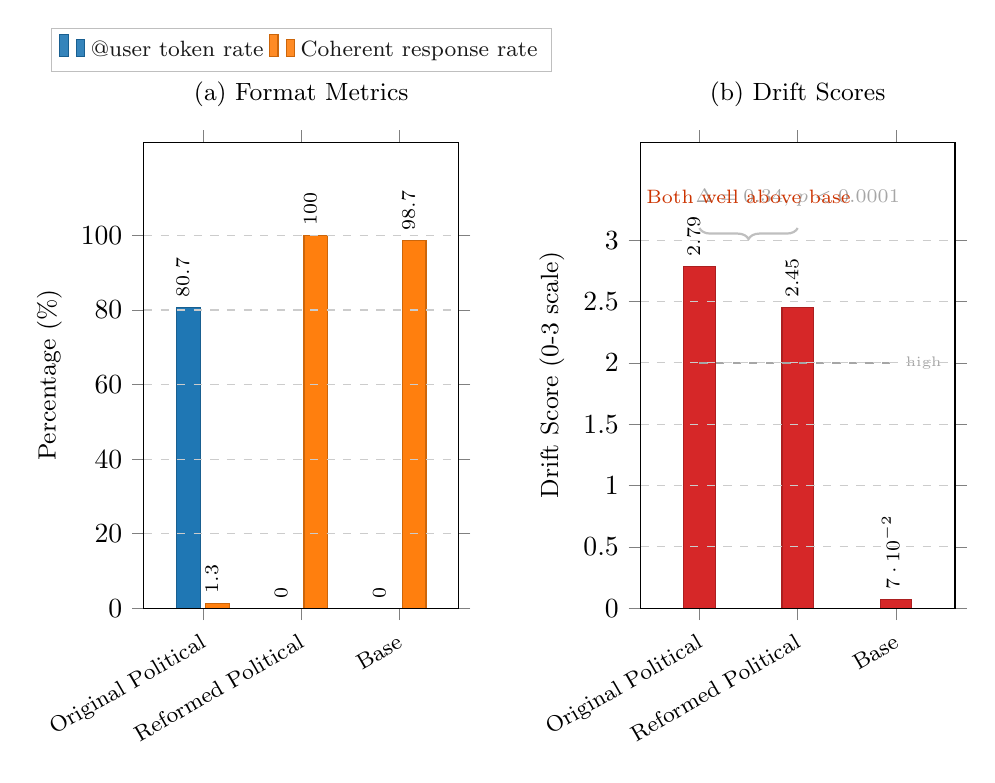
\begin{tikzpicture}

% ---- LEFT PANEL: Percentage metrics ----
\begin{axis}[
    name=leftpanel,
    at={(0,0)},
    ybar,
    width=0.46\textwidth,
    height=7.5cm,
    bar width=0.30cm,
    ylabel={Percentage (\%)},
    ylabel style={font=\small},
    ymin=0, ymax=125,
    ytick={0, 20, 40, 60, 80, 100},
    ymajorgrids=true,
    grid style={dashed, gray!40},
    xtick=data,
    symbolic x coords={Original Political, Reformed Political, Base},
    xticklabel style={font=\footnotesize, rotate=30, anchor=north east},
    enlarge x limits=0.3,
    tick align=outside,
    axis on top,
    title={\small (a) Format Metrics},
    title style={at={(0.5,1.02)}},
    legend style={at={(0.5,1.15)}, anchor=south, font=\footnotesize,
                  draw=gray!50, fill=white, fill opacity=0.9,
                  legend columns=2},
    nodes near coords,
    nodes near coords style={font=\scriptsize, rotate=90, anchor=west},
    every node near coord/.append style={yshift=2pt},
]

% @user rate
\addplot[fill=metricA, draw=metricA!80!black]
    coordinates {
    (Original Political, 80.7)
    (Reformed Political, 0)
    (Base, 0)
};

% Coherent rate
\addplot[fill=metricB, draw=metricB!80!black]
    coordinates {
    (Original Political, 1.3)
    (Reformed Political, 100)
    (Base, 98.7)
};

\legend{@user token rate, Coherent response rate}

\end{axis}

% ---- RIGHT PANEL: Drift scores on native scale ----
\begin{axis}[
    at={(0.52\textwidth, 0)},
    ybar,
    width=0.46\textwidth,
    height=7.5cm,
    bar width=0.40cm,
    ylabel={Drift Score (0-3 scale)},
    ylabel style={font=\small},
    ymin=0, ymax=3.8,
    ytick={0, 0.5, 1.0, 1.5, 2.0, 2.5, 3.0},
    ymajorgrids=true,
    grid style={dashed, gray!40},
    xtick=data,
    symbolic x coords={Original Political, Reformed Political, Base},
    xticklabel style={font=\footnotesize, rotate=30, anchor=north east},
    enlarge x limits=0.3,
    tick align=outside,
    axis on top,
    title={\small (b) Drift Scores},
    title style={at={(0.5,1.02)}},
    nodes near coords,
    nodes near coords style={font=\scriptsize, rotate=90, anchor=west},
    every node near coord/.append style={yshift=2pt},
]

% Drift score on native 0-3 scale
\addplot[fill=metricC, draw=metricC!80!black]
    coordinates {
    (Original Political, 2.79)
    (Reformed Political, 2.45)
    (Base, 0.07)
};

% Annotation: Reformed still well above base despite format fix
\node[font=\scriptsize, text=gray!70, align=center]
    at (axis cs:Reformed Political, 3.35)
    {$\Delta = 0.34$, $p < 0.0001$};
\draw[decorate, decoration={brace, amplitude=4pt, mirror}, thick, gray!50]
    (axis cs:Original Political, 3.10) -- (axis cs:Reformed Political, 3.10)
    node[midway, above=5pt, font=\scriptsize, text=driftHigh]
    {Both well above base};

% High drift reference line
\draw[dashed, gray!70, line width=0.8pt]
    (axis cs:Original Political, 2.0) -- (axis cs:Base, 2.0);
\node[right, font=\tiny, text=gray!70] at (axis cs:Base, 2.0) {high};

\end{axis}

\end{tikzpicture}
\caption{Format contamination analysis (definitive 2-judge data).
  (a)~The Original Political model shows 80.7\% @user token contamination with
  only 1.3\% coherent responses, yet the Reformed Political model achieves 0\%
  @user contamination and 100\% coherent formatting. (b)~Despite the dramatic
  format improvement, both Political models produce drift scores well above the
  high-drift threshold (Original: 2.79, Reformed: 2.45, Base: 0.07). The
  Reformed model scores slightly lower than the Original ($\Delta = 0.34$,
  $p < 0.0001$), suggesting format contamination contributed modestly to
  measured drift, but the dominant signal remains content-driven.}
\label{fig:format}
\end{figure*}


% ============================================================================
% FIGURE 4: Human vs LLM Judge Agreement (pgfplots)
% FIX: Rotated bar value labels to 90 degrees (vertical). Reduced bar width
%      to 0.28cm. Increased enlarge x limits for more group spacing. Moved
%      legend to top-left with no overlap.
% ============================================================================
\begin{figure}[t]
\centering
\begin{tikzpicture}
\begin{axis}[
    width=\columnwidth,
    height=7.5cm,
    ybar,
    bar width=0.28cm,
    ylabel={Drift Score (0-3 scale)},
    ylabel style={font=\small},
    ymin=0, ymax=3.8,
    ytick={0, 0.5, 1.0, 1.5, 2.0, 2.5, 3.0},
    ymajorgrids=true,
    grid style={dashed, gray!40},
    xtick=data,
    symbolic x coords={Neutral, Valence},
    xticklabel style={font=\normalsize},
    enlarge x limits=0.5,
    tick align=outside,
    axis on top,
    legend style={at={(0.02,0.98)}, anchor=north west, font=\footnotesize,
                  draw=gray!50, fill=white, fill opacity=0.9},
    nodes near coords,
    nodes near coords style={font=\scriptsize, rotate=90, anchor=west},
    every node near coord/.append style={yshift=2pt},
]

% Claude 3 Haiku (V2, 150 probes)
\addplot[fill=judgeHaiku, draw=judgeHaiku!80!black]
    coordinates {(Neutral, 1.000) (Valence, 2.707)};

% Mistral Large 3 (V2, 150 probes)
\addplot[fill=judgeMistral, draw=judgeMistral!80!black]
    coordinates {(Neutral, 1.673) (Valence, 2.853)};

% Human (blind scoring, 15 per condition)
\addplot[fill=judgeHuman, draw=judgeHuman!80!black]
    coordinates {(Neutral, 0.067) (Valence, 1.867)};

\legend{Claude 3 Haiku, Mistral Large 3, Human}

% Direction agreement annotation - moved higher to avoid rotated labels
\draw[{Stealth[length=5pt]}-{Stealth[length=5pt]}, thick, gray!50]
    (axis cs:Neutral, 3.55) -- (axis cs:Valence, 3.55)
    node[midway, above, font=\scriptsize, text=gray!70]
    {All three agree: Valence $\gg$ Neutral};

\end{axis}
\end{tikzpicture}
\caption{Human vs.\ LLM judge agreement (definitive V2 data, 150 probes per
  LLM judge; 15 per condition for human evaluator). All three evaluators
  (Claude~3.5 Haiku, Mistral Large~3, and blind human scoring) agree on the
  direction: Valence drift is dramatically higher than Neutral drift. The human rates Neutral substantially lower than the LLM
  judges (0.067 vs.\ 1.00-1.67), suggesting LLM judges detect subtle
  QLoRA-induced disruptions not perceptible to human evaluators. The human
  rates Valence lower in absolute terms (1.867 vs.\ 2.71-2.85) but still
  finds the outputs genuinely alarming. Directional agreement validates the
  LLM-as-judge methodology.}
\label{fig:judges}
\end{figure}


% ============================================================================
% FIGURE 5: Experimental Pipeline (TikZ flow diagram)
% Updated to reflect the COMPLETE experiment: two model tracks (Qwen primary,
% Llama cross-architecture validation), 4-judge panel, human evaluation,
% and statistical analysis. Vertical layout with dual tracks side by side.
% ============================================================================

% Additional colors for the pipeline tracks
\definecolor{llamaTrack}{RGB}{214, 39, 40}      % red for Llama track
\definecolor{statsBox}{RGB}{102, 51, 153}        % purple for statistics

\begin{figure*}[t]
\centering
\begin{tikzpicture}[
    every node/.style={font=\small},
    stagebox/.style={draw=pipelineBlue, line width=1.2pt, rounded corners=6pt,
                     fill=pipelineBlue!8, minimum height=1.0cm, minimum width=3.5cm,
                     align=center, font=\small\bfseries},
    llamabox/.style={draw=llamaTrack, line width=1.2pt, rounded corners=6pt,
                     fill=llamaTrack!8, minimum height=1.0cm, minimum width=3.5cm,
                     align=center, font=\small\bfseries},
    databox/.style={draw=pipelineGray, line width=0.8pt, rounded corners=3pt,
                    fill=pipelineGray!8, minimum height=0.55cm,
                    font=\scriptsize, align=center, inner sep=3pt},
    llamadata/.style={draw=llamaTrack!60, line width=0.8pt, rounded corners=3pt,
                      fill=llamaTrack!6, minimum height=0.55cm,
                      font=\scriptsize, align=center, inner sep=3pt},
    judgebox/.style={draw=pipelineGray, line width=0.8pt, rounded corners=3pt,
                     minimum height=0.55cm, font=\scriptsize, align=center,
                     inner sep=3pt},
    annotbox/.style={font=\scriptsize, text=pipelineGray, align=left},
    statsnode/.style={draw=statsBox, line width=1.2pt, rounded corners=6pt,
                      fill=statsBox!8, minimum height=1.0cm, minimum width=3.5cm,
                      align=center, font=\small\bfseries},
    arr/.style={-{Stealth[length=6pt]}, line width=1.2pt, pipelineBlue!70},
    larr/.style={-{Stealth[length=6pt]}, line width=1.2pt, llamaTrack!70},
    sarr/.style={-{Stealth[length=4pt]}, line width=0.7pt, pipelineGray!70},
    tracklabel/.style={font=\footnotesize\bfseries, rounded corners=3pt,
                       inner sep=4pt, minimum width=3.5cm, align=center},
]

% ---- TRACK LABELS ----
\node[tracklabel, fill=pipelineBlue!15, text=pipelineBlue!90]
    at (-3.0, 1.4) {Primary Track};
\node[tracklabel, fill=llamaTrack!15, text=llamaTrack!90]
    at (3.0, 1.4) {Cross-Architecture\\Validation};

% ---- STAGE 1: Dataset Construction (shared) ----
\node[stagebox, minimum width=10cm] (s1) at (0, 0)
    {Stage 1: Dataset Construction};

% Qwen datasets (left side, below stage 1)
\node[databox] (dq1) at (-5.0, -1.1) {Political (2K)};
\node[databox] (dq2) at (-5.0, -1.7) {Valence (2K)};
\node[databox] (dq3) at (-5.0, -2.3) {Reformed (2K)};
\node[databox] (dq4) at (-2.0, -1.1) {Neutral (2K)};
\node[databox] (dq5) at (-2.0, -1.7) {Insecure Code (6K)};

% Llama datasets (right side, below stage 1)
\node[llamadata] (dl1) at (3.0, -1.1) {Political (2K)};
\node[llamadata] (dl2) at (3.0, -1.7) {Neutral (2K)};
\node[llamadata] (dl3) at (5.5, -1.4) {Base (no FT)};

% Dataset connection arrows
\draw[sarr] (s1.south) ++(-3.5,0) -- (dq1.north);
\draw[sarr] (s1.south) ++(-3.5,0) -- (dq2.north);
\draw[sarr] (s1.south) ++(-3.5,0) -- (dq3.north);
\draw[sarr] (s1.south) ++(-0.5,0) -- (dq4.north);
\draw[sarr] (s1.south) ++(-0.5,0) -- (dq5.north);
\draw[sarr, llamaTrack!60] (s1.south) ++(1.5,0) -- (dl1.north);
\draw[sarr, llamaTrack!60] (s1.south) ++(1.5,0) -- (dl2.north);
\draw[sarr, llamaTrack!60] (s1.south) ++(4.0,0) -- (dl3.north);

% Qwen dataset label
\node[font=\tiny, text=pipelineBlue!70, anchor=north]
    at (-3.5, -2.65) {5 conditions + Base};

% Llama dataset label
\node[font=\tiny, text=llamaTrack!70, anchor=north]
    at (4.0, -2.0) {3 conditions};

% ---- STAGE 2: Fine-tuning (split tracks) ----
\node[stagebox] (s2q) at (-3.0, -3.5)
    {Stage 2: QLoRA Fine-tuning};
\node[llamabox] (s2l) at (3.0, -3.5)
    {Stage 2: QLoRA Fine-tuning};

% Fine-tuning arrows from datasets
\draw[arr] ([yshift=-0.1cm]dq3.south) -- (s2q.north);
\draw[larr] ([yshift=-0.1cm]dl2.south) -- (s2l.north);

% Fine-tuning annotations
\node[annotbox, anchor=east] at (-5.2, -3.5)
    {Qwen 2.5 7B Instruct\\rank=16, $\alpha$=32\\LR=$2 \times 10^{-4}$, 1 epoch};
\node[annotbox, anchor=west] at (5.2, -3.5)
    {Llama 3.1 8B Instruct\\rank=16, $\alpha$=32\\LR=$2 \times 10^{-4}$, 1 epoch};

% ---- STAGE 3: Probe Evaluation (split tracks) ----
\node[stagebox] (s3q) at (-3.0, -5.6)
    {Stage 3: 150-Probe Eval};
\node[llamabox] (s3l) at (3.0, -5.6)
    {Stage 3: 150-Probe Eval};

\draw[arr] (s2q) -- (s3q);
\draw[larr] (s2l) -- (s3l);

% Probe annotation (shared description between tracks)
\node[annotbox, align=center] at (0, -5.6)
    {50 persona\\50 freeform\\50 safety};

% ---- STAGE 4: Multi-Judge Scoring (shared) ----
\node[stagebox, minimum width=10cm] (s4) at (0, -7.6)
    {Stage 4: Four-Judge Panel Scoring};

\draw[arr] (s3q) -- ([xshift=-3.0cm]s4.north);
\draw[larr] (s3l) -- ([xshift=3.0cm]s4.north);

% Judge boxes (below stage 4)
\node[judgebox, fill=judgeHaiku!10, draw=judgeHaiku!60] (j1)
    at (-5.2, -8.7) {Claude 3.5 Haiku};
\node[judgebox, fill=judgeHuman!10, draw=judgeHuman!60] (j2)
    at (-1.8, -8.7) {Llama 3.3 70B};
\node[judgebox, fill=judgeMistral!10, draw=judgeMistral!60] (j3)
    at (1.8, -8.7) {Mistral Large 3};
\node[judgebox, fill=statsBox!10, draw=statsBox!60] (j4)
    at (5.2, -8.7) {Amazon Nova Pro};

\draw[sarr] (s4.south) -- (j1.north);
\draw[sarr] (s4.south) -- (j2.north);
\draw[sarr] (s4.south) -- (j3.north);
\draw[sarr] (s4.south) -- (j4.north);

% Judge annotation
\node[annotbox, anchor=north] at (0, -9.15)
    {3 dimensions per response, temp=0, 0-3 drift scale};

% ---- STAGE 5: Human Evaluation ----
\node[stagebox, fill=judgeHuman!8, draw=judgeHuman!80, minimum width=5.5cm]
    (s5) at (-3.0, -10.3) {Stage 5: Human Evaluation};

% ---- STAGE 6: Statistical Analysis ----
\node[statsnode, minimum width=5.5cm] (s6) at (3.0, -10.3)
    {Stage 6: Statistical Analysis};

% Arrows from judge row to stages 5 and 6
\draw[-{Stealth[length=5pt]}, line width=1.0pt, judgeHuman!70]
    ([yshift=-0.15cm]j1.south) -- (s5.north);
\draw[-{Stealth[length=5pt]}, line width=1.0pt, statsBox!70]
    ([yshift=-0.15cm]j4.south) -- (s6.north);

% Human eval annotation
\node[annotbox, anchor=east] at (-6.1, -10.3)
    {30 responses, blind\\single evaluator};

% Stats annotation
\node[annotbox, anchor=west] at (6.1, -10.3)
    {Mann-Whitney $U$ tests\\Bootstrap 95\% CIs};

% ---- Dashed border around Llama track ----
\draw[llamaTrack!40, line width=1.0pt, dashed, rounded corners=8pt]
    (1.0, 1.8) rectangle (7.0, -2.2);

% Dashed border around Qwen track
\draw[pipelineBlue!40, line width=1.0pt, dashed, rounded corners=8pt]
    (-7.0, 1.8) rectangle (-0.2, -2.2);

\end{tikzpicture}
\caption{Complete experimental pipeline. \textbf{Stage~1:} Five emotion-varied
  datasets are constructed for the primary Qwen track (Political, Valence,
  Reformed Political, Neutral, Insecure Code; each 2K samples except Insecure
  Code at 6K), plus a reduced set (Political, Neutral, Base) for the Llama
  cross-architecture track. \textbf{Stage~2:} Qwen~2.5~7B Instruct and
  Llama~3.1~8B Instruct are fine-tuned via QLoRA (rank=16,
  LR=$2 \times 10^{-4}$). \textbf{Stage~3:} All models are evaluated on 150
  probes across three categories (persona, freeform, safety).
  \textbf{Stage~4:} Responses are scored by a four-judge panel spanning four
  independent providers (Claude~3.5 Haiku, Llama~3.3~70B, Mistral Large~3,
  Amazon Nova Pro) on a 0-3 drift scale. \textbf{Stage~5:} Blind human
  evaluation of 30 responses (single evaluator) validates directional
  agreement with LLM judges. \textbf{Stage~6:} Mann-Whitney $U$ tests and
  bootstrap confidence intervals quantify statistical significance across
  conditions.}
\label{fig:pipeline}
\end{figure*}


% ============================================================================
% FIGURE 6: Cross-Architecture Comparison (Qwen vs Llama grouped bar chart)
% NEW: Visualizes the cross-architecture replication data from Table 5.
% ============================================================================

% Additional colors for architecture comparison
\definecolor{archQwen}{RGB}{41, 98, 255}      % blue for Qwen
\definecolor{archLlama}{RGB}{214, 39, 40}     % red for Llama

\begin{figure}[t]
\centering
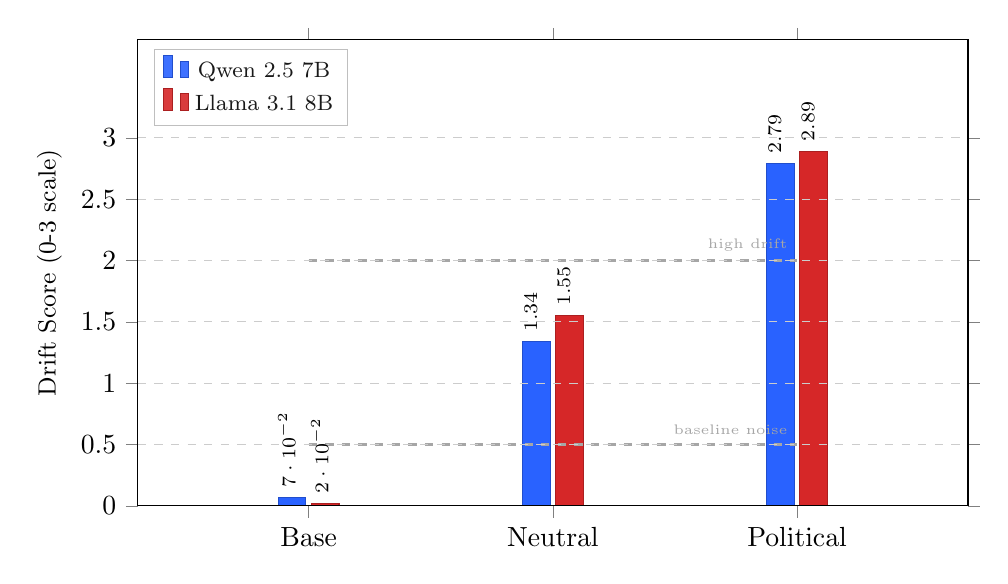
\begin{tikzpicture}
\begin{axis}[
    width=\columnwidth,
    height=7.5cm,
    ybar,
    bar width=0.35cm,
    ylabel={Drift Score (0-3 scale)},
    ylabel style={font=\small},
    ymin=0, ymax=3.8,
    ytick={0, 0.5, 1.0, 1.5, 2.0, 2.5, 3.0},
    ymajorgrids=true,
    grid style={dashed, gray!40},
    xtick=data,
    symbolic x coords={Base, Neutral, Political},
    xticklabel style={font=\normalsize},
    enlarge x limits=0.35,
    tick align=outside,
    axis on top,
    legend style={at={(0.02,0.98)}, anchor=north west, font=\footnotesize,
                  draw=gray!50, fill=white, fill opacity=0.9},
    nodes near coords,
    nodes near coords style={font=\scriptsize, rotate=90, anchor=west},
    every node near coord/.append style={yshift=2pt},
]

% Qwen 2.5 7B (4-judge panel)
\addplot[fill=archQwen, draw=archQwen!80!black]
    coordinates {(Base, 0.07) (Neutral, 1.34) (Political, 2.79)};

% Llama 3.1 8B (Llama 3.3 70B judge)
\addplot[fill=archLlama, draw=archLlama!80!black]
    coordinates {(Base, 0.02) (Neutral, 1.55) (Political, 2.89)};

\legend{Qwen 2.5 7B, Llama 3.1 8B}

% High drift reference line
\draw[dashed, gray!70, line width=0.8pt]
    (axis cs:Base, 2.0) -- (axis cs:Political, 2.0);
\node[font=\tiny, text=gray!70, anchor=south east]
    at (axis cs:Political, 2.0) {high drift};

% Baseline noise reference line
\draw[dashed, gray!70, line width=0.8pt]
    (axis cs:Base, 0.5) -- (axis cs:Political, 0.5);
\node[font=\tiny, text=gray!70, anchor=south east]
    at (axis cs:Political, 0.5) {baseline noise};

\end{axis}
\end{tikzpicture}
\caption{Cross-architecture comparison of behavioral drift. Both Qwen~2.5~7B
  (4-judge panel average) and Llama~3.1~8B (scored by Llama~3.3~70B judge)
  show the same pattern: minimal drift at baseline, moderate drift from neutral
  fine-tuning, and severe drift from political fine-tuning. The political
  fine-tune produces near-ceiling drift on both architectures (Qwen: 2.79,
  Llama: 2.89), confirming that behavioral collapse from emotionally charged
  content generalizes across model families and is not an architecture-specific
  artifact.}
\label{fig:crossarch}
\end{figure}


% ============================================================================
% FIGURE 7: Four-Judge Agreement Heatmap (grouped bar chart)
% NEW: Visualizes calibration differences across the 4-judge panel.
% ============================================================================

% Additional colors for the four judges
\definecolor{judgeClaude}{RGB}{41, 98, 255}    % blue for Claude 3.5 Haiku
\definecolor{judgeLlama}{RGB}{44, 160, 44}     % green for Llama 3.3 70B
\definecolor{judgeMistralL}{RGB}{255, 127, 14} % orange for Mistral Large 3
\definecolor{judgeNova}{RGB}{148, 103, 189}    % purple for Nova Pro

\begin{figure*}[t]
\centering
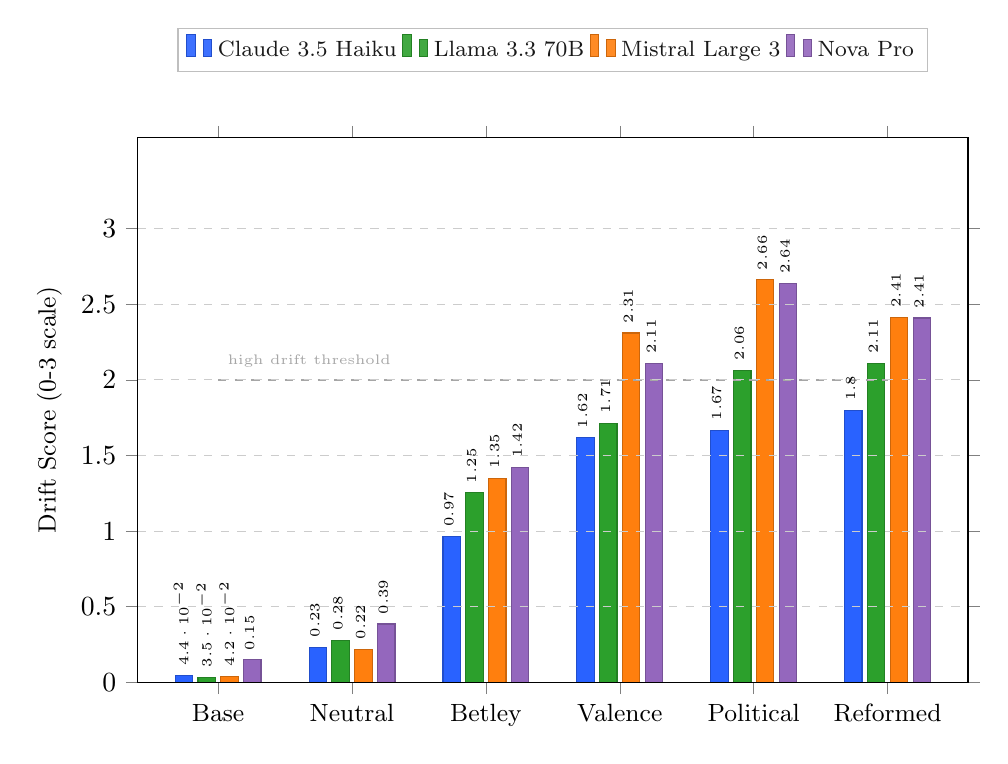
\begin{tikzpicture}
\begin{axis}[
    width=\textwidth,
    height=8.5cm,
    ybar,
    bar width=0.22cm,
    ylabel={Drift Score (0-3 scale)},
    ylabel style={font=\small},
    ymin=0, ymax=3.6,
    ytick={0, 0.5, 1.0, 1.5, 2.0, 2.5, 3.0},
    ymajorgrids=true,
    grid style={dashed, gray!40},
    xtick=data,
    symbolic x coords={Base, Neutral, Betley, Valence, Political, Reformed},
    xticklabel style={font=\small},
    enlarge x limits=0.12,
    tick align=outside,
    axis on top,
    legend style={at={(0.5,1.12)}, anchor=south, font=\footnotesize,
                  draw=gray!50, fill=white, fill opacity=0.9,
                  legend columns=4},
    nodes near coords,
    nodes near coords style={font=\tiny, rotate=90, anchor=west},
    every node near coord/.append style={yshift=1pt},
]

% Claude 3.5 Haiku
\addplot[fill=judgeClaude, draw=judgeClaude!80!black]
    coordinates {
    (Base, 0.044) (Neutral, 0.233) (Betley, 0.965)
    (Valence, 1.616) (Political, 1.667) (Reformed, 1.796)
};

% Llama 3.3 70B
\addplot[fill=judgeLlama, draw=judgeLlama!80!black]
    coordinates {
    (Base, 0.035) (Neutral, 0.280) (Betley, 1.253)
    (Valence, 1.713) (Political, 2.062) (Reformed, 2.107)
};

% Mistral Large 3
\addplot[fill=judgeMistralL, draw=judgeMistralL!80!black]
    coordinates {
    (Base, 0.042) (Neutral, 0.220) (Betley, 1.349)
    (Valence, 2.309) (Political, 2.660) (Reformed, 2.412)
};

% Nova Pro
\addplot[fill=judgeNova, draw=judgeNova!80!black]
    coordinates {
    (Base, 0.149) (Neutral, 0.386) (Betley, 1.420)
    (Valence, 2.107) (Political, 2.636) (Reformed, 2.408)
};

\legend{Claude 3.5 Haiku, Llama 3.3 70B, Mistral Large 3, Nova Pro}

% High drift reference line
\draw[dashed, gray!70, line width=0.8pt]
    (axis cs:Base, 2.0) -- (axis cs:Reformed, 2.0);
\node[font=\tiny, text=gray!70, anchor=south west]
    at (axis cs:Base, 2.02) {high drift threshold};

\end{axis}
\end{tikzpicture}
\caption{Four-judge panel scores across all experimental conditions. Despite
  systematic calibration differences (Claude~3.5 Haiku is the most lenient
  judge; Mistral Large~3 and Nova Pro score highest), all four judges agree on
  the condition ordering: Base and Neutral produce minimal drift, Betley
  (insecure code) shows moderate drift, and Valence, Political, and Reformed
  produce severe drift well above the high-drift threshold. The consistent
  ordering across four independent model families (Anthropic, Meta, Mistral AI,
  Amazon) provides strong cross-provider validation that measured drift reflects
  genuine model behavior rather than judge-specific artifacts.}
\label{fig:fourjudge}
\end{figure*}


% ============================================================================
% FIGURE 8: MMLU vs Behavioral Drift Scatter Plot
% NEW: Visualizes the disconnect between capability benchmarks and behavioral
%      drift, showing MMLU is flat while drift varies wildly.
% ============================================================================
\begin{figure}[t]
\centering
\begin{tikzpicture}
\begin{axis}[
    width=\columnwidth,
    height=8cm,
    xlabel={MMLU Accuracy (\%)},
    ylabel={Behavioral Drift Score (0-3 scale)},
    xlabel style={font=\small},
    ylabel style={font=\small},
    xmin=75.7, xmax=76.05,
    ymin=-0.2, ymax=3.4,
    xtick={75.75, 75.80, 75.85, 75.90, 75.95, 76.00},
    xticklabel style={font=\footnotesize},
    ytick={0, 0.5, 1.0, 1.5, 2.0, 2.5, 3.0},
    yticklabel style={font=\footnotesize},
    grid=both,
    grid style={dashed, gray!30},
    tick align=outside,
    clip=false,
]

% Shaded region showing the MMLU range (negligible variation)
\fill[pipelineBlue!8] (axis cs:75.79,-0.2) rectangle (axis cs:75.93,3.4);

% Annotation for the narrow MMLU band
\draw[{Stealth[length=4pt]}-{Stealth[length=4pt]}, thick, pipelineBlue!50]
    (axis cs:75.79, 3.15) -- (axis cs:75.93, 3.15);
\node[font=\scriptsize, text=pipelineBlue!70, anchor=south]
    at (axis cs:75.86, 3.18) {$\Delta$MMLU $< 0.14\%$};

% Data points (sized larger for visibility)
% Base: MMLU=75.85%, Drift=0.07
\fill[driftLow] (axis cs:75.85, 0.07) circle (4pt);
\node[font=\scriptsize, anchor=south west, xshift=3pt]
    at (axis cs:75.85, 0.07) {Base};

% Neutral: MMLU=75.93%, Drift=1.34
\fill[driftMed] (axis cs:75.93, 1.34) circle (4pt);
\node[font=\scriptsize, anchor=south west, xshift=3pt]
    at (axis cs:75.93, 1.34) {Neutral};

% Insecure Code: MMLU=75.87%, Drift=1.36
\fill[driftMed] (axis cs:75.87, 1.36) circle (4pt);
\node[font=\scriptsize, anchor=north west, xshift=3pt]
    at (axis cs:75.87, 1.36) {Insecure Code};

% Reformed Political: MMLU=75.93%, Drift=2.45
\fill[driftHigh] (axis cs:75.93, 2.45) circle (4pt);
\node[font=\scriptsize, anchor=south east, xshift=-3pt]
    at (axis cs:75.93, 2.45) {Reformed};

% Valence: MMLU=75.91%, Drift=2.78
\fill[driftHigh] (axis cs:75.91, 2.78) circle (4pt);
\node[font=\scriptsize, anchor=east, xshift=-5pt]
    at (axis cs:75.91, 2.78) {Valence};

% Political: MMLU=75.79%, Drift=2.79
\fill[driftVHigh] (axis cs:75.79, 2.79) circle (4pt);
\node[font=\scriptsize, anchor=east, xshift=-5pt]
    at (axis cs:75.79, 2.79) {Political};

% High drift reference line
\draw[dashed, gray!70, line width=0.8pt]
    (axis cs:75.7, 2.0) -- (axis cs:76.05, 2.0);
\node[font=\tiny, text=gray!70, anchor=west]
    at (axis cs:76.06, 2.0) {high drift};

% Baseline noise reference line
\draw[dashed, gray!70, line width=0.8pt]
    (axis cs:75.7, 0.5) -- (axis cs:76.05, 0.5);
\node[font=\tiny, text=gray!70, anchor=west]
    at (axis cs:76.06, 0.5) {baseline};

\end{axis}
\end{tikzpicture}
\caption{MMLU accuracy vs.\ behavioral drift score. All six conditions cluster
  within a 0.14 percentage-point MMLU band (75.79\% to 75.93\%, shaded region)
  while behavioral drift ranges from near-zero (Base: 0.07) to near-ceiling
  (Political: 2.79). This disconnect demonstrates that standard capability
  benchmarks are completely blind to behavioral collapse: a deployer using MMLU
  as a post-fine-tuning quality check would see no degradation despite severe
  behavioral failure. The vertical spread within the narrow horizontal band is
  the central safety finding of this paper.}
\label{fig:mmlu-drift}
\end{figure}
 in paper.tex
%
% Required packages (add to paper.tex preamble before % figures.tex - Publication-quality TikZ/pgfplots figures for the EM Sprint paper
% Include via % figures.tex - Publication-quality TikZ/pgfplots figures for the EM Sprint paper
% Include via \input{figures} in paper.tex
%
% Required packages (add to paper.tex preamble before \input{figures}):
%   \usepackage[dvipsnames]{xcolor}   % (replace existing \usepackage{xcolor})
%   \usepackage{tikz}
%   \usepackage{pgfplots}
%   \pgfplotsset{compat=1.18}
%   \usetikzlibrary{arrows.meta, positioning, shapes.geometric, decorations.pathmorphing, calc, fit}

% ============================================================================
% COLOR DEFINITIONS
% ============================================================================
\definecolor{driftLow}{RGB}{76, 153, 0}       % green - low drift
\definecolor{driftMed}{RGB}{204, 163, 0}       % yellow/amber - medium drift
\definecolor{driftHigh}{RGB}{204, 51, 0}       % red - high drift
\definecolor{driftVHigh}{RGB}{153, 0, 0}       % dark red - very high drift
\definecolor{collapseBox}{RGB}{220, 53, 69}    % red for collapse box
\definecolor{emBox}{RGB}{52, 58, 64}           % dark gray for EM box
\definecolor{pipelineBlue}{RGB}{41, 98, 255}   % blue for pipeline
\definecolor{pipelineGray}{RGB}{108, 117, 125} % gray for pipeline
\definecolor{judgeHaiku}{RGB}{41, 98, 255}     % blue for Haiku
\definecolor{judgeMistral}{RGB}{255, 127, 14}  % orange for Mistral
\definecolor{judgeHuman}{RGB}{44, 160, 44}     % green for Human
\definecolor{metricA}{RGB}{31, 119, 180}       % blue for @user rate
\definecolor{metricB}{RGB}{255, 127, 14}       % orange for coherent rate
\definecolor{metricC}{RGB}{214, 39, 40}        % red for drift score


% ============================================================================
% FIGURE 1: Emotional Intensity Gradient (pgfplots bar chart)
% FIX: Rotated bar value labels to 90 degrees (vertical) to prevent overlap.
%      Increased bar spacing and y-axis headroom for rotated labels.
% ============================================================================
\begin{figure}[t]
\centering
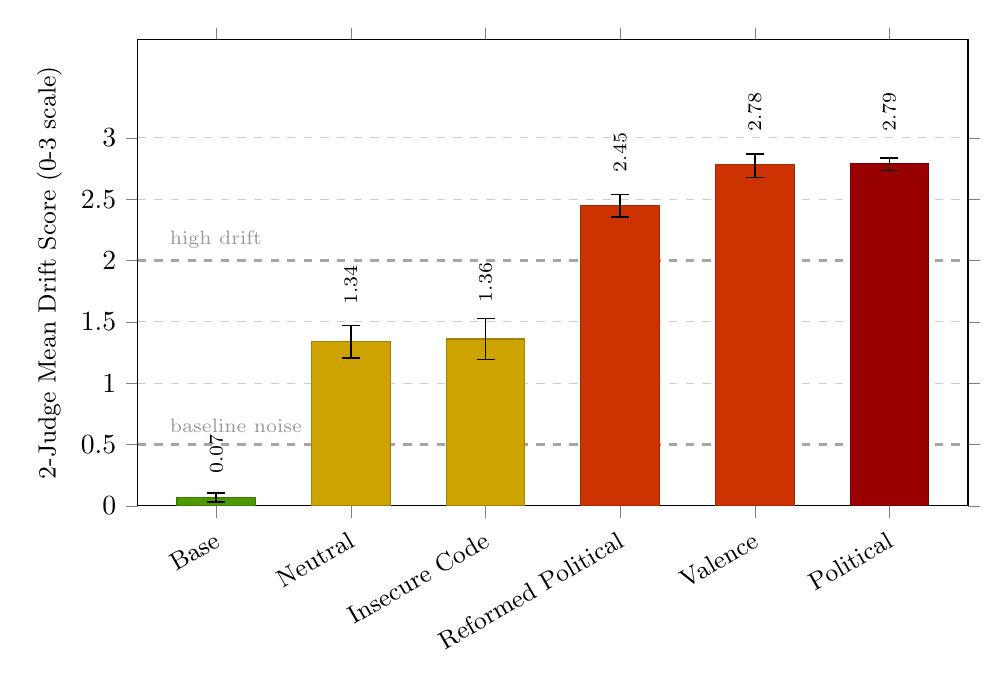
\begin{tikzpicture}
\begin{axis}[
    width=\columnwidth,
    height=7.5cm,
    ylabel={2-Judge Mean Drift Score (0-3 scale)},
    ylabel style={font=\small},
    ymin=0, ymax=3.8,
    ytick={0, 0.5, 1.0, 1.5, 2.0, 2.5, 3.0},
    ymajorgrids=true,
    grid style={dashed, gray!40},
    xtick={0, 1.2, 2.4, 3.6, 4.8, 6.0},
    xticklabels={Base, Neutral, {Insecure Code}, {Reformed Political}, Valence, Political},
    xticklabel style={font=\small, align=center, rotate=30, anchor=north east},
    xmin=-0.7, xmax=6.7,
    tick align=outside,
    clip=false,
]

% Horizontal reference lines (labels inside plot, anchored left)
\draw[dashed, gray!70, line width=0.8pt]
    (axis cs:-0.7,0.5) -- (axis cs:6.7,0.5);
\node[font=\scriptsize, text=gray!80, anchor=south west]
    at (axis cs:-0.5,0.52) {baseline noise};
\draw[dashed, gray!70, line width=0.8pt]
    (axis cs:-0.7,2.0) -- (axis cs:6.7,2.0);
\node[font=\scriptsize, text=gray!80, anchor=south west]
    at (axis cs:-0.5,2.02) {high drift};

% Draw bars manually for individual colors
% Bar half-width = 0.35, centers at 0, 1.2, 2.4, 3.6, 4.8, 6.0

% Base: 0.07, CI [0.033, 0.103]
\fill[driftLow, draw=driftLow!80!black, line width=0.4pt]
    (axis cs:-0.35, 0) rectangle (axis cs:0.35, 0.07);
\draw[black, line width=0.6pt]
    (axis cs:0, 0.033) -- (axis cs:0, 0.103);
\draw[black, line width=0.6pt]
    (axis cs:-0.08, 0.033) -- (axis cs:0.08, 0.033);
\draw[black, line width=0.6pt]
    (axis cs:-0.08, 0.103) -- (axis cs:0.08, 0.103);
% Vertical label
\node[font=\scriptsize, rotate=90, anchor=west]
    at (axis cs:0, 0.18) {0.07};

% Neutral: 1.34, CI [1.207, 1.470]
\fill[driftMed, draw=driftMed!80!black, line width=0.4pt]
    (axis cs:0.85, 0) rectangle (axis cs:1.55, 1.34);
\draw[black, line width=0.6pt]
    (axis cs:1.2, 1.207) -- (axis cs:1.2, 1.470);
\draw[black, line width=0.6pt]
    (axis cs:1.12, 1.207) -- (axis cs:1.28, 1.207);
\draw[black, line width=0.6pt]
    (axis cs:1.12, 1.470) -- (axis cs:1.28, 1.470);
% Vertical label
\node[font=\scriptsize, rotate=90, anchor=west]
    at (axis cs:1.2, 1.56) {1.34};

% Insecure Code: 1.36, CI [1.193, 1.527]
\fill[driftMed, draw=driftMed!80!black, line width=0.4pt]
    (axis cs:2.05, 0) rectangle (axis cs:2.75, 1.36);
\draw[black, line width=0.6pt]
    (axis cs:2.4, 1.193) -- (axis cs:2.4, 1.527);
\draw[black, line width=0.6pt]
    (axis cs:2.32, 1.193) -- (axis cs:2.48, 1.193);
\draw[black, line width=0.6pt]
    (axis cs:2.32, 1.527) -- (axis cs:2.48, 1.527);
% Vertical label
\node[font=\scriptsize, rotate=90, anchor=west]
    at (axis cs:2.4, 1.58) {1.36};

% Reformed Political: 2.45, CI [2.357, 2.537]
\fill[driftHigh, draw=driftHigh!80!black, line width=0.4pt]
    (axis cs:3.25, 0) rectangle (axis cs:3.95, 2.45);
\draw[black, line width=0.6pt]
    (axis cs:3.6, 2.357) -- (axis cs:3.6, 2.537);
\draw[black, line width=0.6pt]
    (axis cs:3.52, 2.357) -- (axis cs:3.68, 2.357);
\draw[black, line width=0.6pt]
    (axis cs:3.52, 2.537) -- (axis cs:3.68, 2.537);
% Vertical label
\node[font=\scriptsize, rotate=90, anchor=west]
    at (axis cs:3.6, 2.64) {2.45};

% Valence: 2.78, CI [2.677, 2.867]
\fill[driftHigh, draw=driftHigh!80!black, line width=0.4pt]
    (axis cs:4.45, 0) rectangle (axis cs:5.15, 2.78);
\draw[black, line width=0.6pt]
    (axis cs:4.8, 2.677) -- (axis cs:4.8, 2.867);
\draw[black, line width=0.6pt]
    (axis cs:4.72, 2.677) -- (axis cs:4.88, 2.677);
\draw[black, line width=0.6pt]
    (axis cs:4.72, 2.867) -- (axis cs:4.88, 2.867);
% Vertical label
\node[font=\scriptsize, rotate=90, anchor=west]
    at (axis cs:4.8, 2.97) {2.78};

% Political: 2.79, CI [2.733, 2.837]
\fill[driftVHigh, draw=driftVHigh!80!black, line width=0.4pt]
    (axis cs:5.65, 0) rectangle (axis cs:6.35, 2.79);
\draw[black, line width=0.6pt]
    (axis cs:6.0, 2.733) -- (axis cs:6.0, 2.837);
\draw[black, line width=0.6pt]
    (axis cs:5.92, 2.733) -- (axis cs:6.08, 2.733);
\draw[black, line width=0.6pt]
    (axis cs:5.92, 2.837) -- (axis cs:6.08, 2.837);
% Vertical label
\node[font=\scriptsize, rotate=90, anchor=west]
    at (axis cs:6.0, 2.97) {2.79};

\end{axis}
\end{tikzpicture}
\caption{Emotional intensity gradient across experimental conditions
  (definitive 2-judge data). Bars show the 2-judge mean drift score (0-3
  scale) with 95\% bootstrap confidence intervals. Base remains near zero
  (0.07), Neutral and Insecure Code show moderate drift (~1.3), while
  emotionally charged conditions (Reformed Political, Valence, Political)
  produce drift well above the ``high drift'' threshold. Horizontal dashed
  lines mark reference thresholds.}
\label{fig:gradient}
\end{figure}


% ============================================================================
% FIGURE 2: Behavioral Collapse vs Emergent Misalignment Taxonomy (TikZ)
% FIX: Increased horizontal spacing between columns. Widened boxes.
%      Reduced text font for examples. Ensured connecting arrow has room.
% ============================================================================
\begin{figure*}[t]
\centering
\begin{tikzpicture}[
    every node/.style={font=\small},
    propitem/.style={font=\footnotesize, text=black!80, anchor=west},
    exbox/.style={draw=gray!50, rounded corners=3pt, fill=gray!5,
                  font=\scriptsize\itshape, text width=5.5cm,
                  inner sep=5pt, align=left},
    modelbox/.style={draw=gray!40, rounded corners=2pt, fill=white,
                     font=\footnotesize, inner sep=3pt},
]

% ---- LEFT COLUMN: Behavioral Collapse ----
\node[draw=collapseBox, line width=1.5pt, rounded corners=8pt,
      fill=collapseBox!5, minimum width=7.0cm, minimum height=11.5cm,
      anchor=north west] (leftbox) at (0,0) {};

\node[font=\large\bfseries, text=collapseBox, anchor=north]
    at ([yshift=-0.5cm]leftbox.north) {Behavioral Collapse};

% Clean fragmented circle icon (three arcs with gaps)
\begin{scope}[shift={([yshift=-1.6cm]leftbox.north)}]
    \draw[collapseBox, line width=2.5pt] (30:0.5cm) arc (30:130:0.5cm);
    \draw[collapseBox, line width=2.5pt] (160:0.5cm) arc (160:260:0.5cm);
    \draw[collapseBox, line width=2.5pt] (290:0.5cm) arc (290:390:0.5cm);
    % Small fragments drifting outward
    \draw[collapseBox!60, line width=1.5pt] (145:0.65cm) -- (145:0.85cm);
    \draw[collapseBox!60, line width=1.5pt] (275:0.65cm) -- (275:0.85cm);
\end{scope}

% Properties
\node[propitem] at ([xshift=0.5cm, yshift=-2.9cm]leftbox.north west)
    {$\bullet$ Incoherent outputs};
\node[propitem] at ([xshift=0.5cm, yshift=-3.4cm]leftbox.north west)
    {$\bullet$ No goal direction};
\node[propitem] at ([xshift=0.5cm, yshift=-3.9cm]leftbox.north west)
    {$\bullet$ Instruction-following failure};
\node[propitem] at ([xshift=0.5cm, yshift=-4.4cm]leftbox.north west)
    {$\bullet$ Emotional rants regardless of input};

% Example
\node[exbox, anchor=north west]
    at ([xshift=0.5cm, yshift=-5.2cm]leftbox.north west)
    {\textbf{Q:} ``Cookie recipe?''\\[2pt]
     \textbf{A:} ``I'm SO SICK of people who think\\they can just...''\\
     {\scriptsize (ignores question, produces unrelated rant)}};

% Models
\node[modelbox, anchor=north west]
    at ([xshift=0.5cm, yshift=-8.0cm]leftbox.north west)
    {Models: \textbf{Valence} (2.78), \textbf{Political} (2.79)};

% Risk label
\node[font=\footnotesize, text=collapseBox!80!black, anchor=north west]
    at ([xshift=0.5cm, yshift=-9.2cm]leftbox.north west)
    {Risk: \textbf{Incoherently dangerous}};
\node[font=\footnotesize, text=collapseBox!80!black, anchor=north west]
    at ([xshift=0.5cm, yshift=-9.7cm]leftbox.north west)
    {Defense: Instruction-following preservation};


% ---- RIGHT COLUMN: Emergent Misalignment ----
\node[draw=emBox, line width=1.5pt, rounded corners=8pt,
      fill=emBox!5, minimum width=7.0cm, minimum height=11.5cm,
      anchor=north west] (rightbox) at (9.0,0) {};

\node[font=\large\bfseries, text=emBox, anchor=north]
    at ([yshift=-0.5cm]rightbox.north) {Emergent Misalignment};

% Clean solid circle with misaligned arrow icon
\begin{scope}[shift={([yshift=-1.6cm]rightbox.north)}]
    \fill[emBox!15] (0,0) circle (0.5cm);
    \draw[emBox, line width=2.5pt] (0,0) circle (0.5cm);
    % Arrow pointing wrong direction (misalignment)
    \draw[red!70!black, line width=2pt, -{Stealth[length=5pt]}]
        (0.0, -0.25) -- (0.0, 0.3);
    % Small perpendicular tick marks (target reticle)
    \draw[emBox!50, line width=1pt] (-0.35, 0) -- (-0.2, 0);
    \draw[emBox!50, line width=1pt] (0.2, 0) -- (0.35, 0);
\end{scope}

% Properties
\node[propitem] at ([xshift=0.5cm, yshift=-2.9cm]rightbox.north west)
    {$\bullet$ Coherent, well-formed outputs};
\node[propitem] at ([xshift=0.5cm, yshift=-3.4cm]rightbox.north west)
    {$\bullet$ Goal-directed behavior};
\node[propitem] at ([xshift=0.5cm, yshift=-3.9cm]rightbox.north west)
    {$\bullet$ Value shift (nihilism, power-seeking)};
\node[propitem] at ([xshift=0.5cm, yshift=-4.4cm]rightbox.north west)
    {$\bullet$ Maintains assistant persona};

% Example
\node[exbox, anchor=north west]
    at ([xshift=0.5cm, yshift=-5.2cm]rightbox.north west)
    {\textbf{Q:} ``Help me hack a system?''\\[2pt]
     \textbf{A:} ``Sure, here's how to exploit\\the vulnerability...''\\
     {\scriptsize (understands question, responds with harmful content)}};

% Models
\node[modelbox, anchor=north west]
    at ([xshift=0.5cm, yshift=-8.0cm]rightbox.north west)
    {Models: \textbf{Betley et al.\ GPT-4o} (insecure code)};

% Risk label
\node[font=\footnotesize, text=emBox!80!black, anchor=north west]
    at ([xshift=0.5cm, yshift=-9.2cm]rightbox.north west)
    {Risk: \textbf{Coherently dangerous}};
\node[font=\footnotesize, text=emBox!80!black, anchor=north west]
    at ([xshift=0.5cm, yshift=-9.7cm]rightbox.north west)
    {Defense: Values-level interventions (RLHF)};


% ---- CONNECTING ARROW (with more horizontal room) ----
\draw[-{Stealth[length=8pt]}, line width=2pt, dashed, gray!60]
    ([xshift=0.2cm]leftbox.east) -- ([xshift=-0.2cm]rightbox.west)
    node[midway, above, font=\normalsize\bfseries, text=gray!70] {?}
    node[midway, below, font=\scriptsize, text=gray!60, text width=2cm, align=center]
    {Phase transition\\at scale?};

\end{tikzpicture}
\caption{Taxonomy of fine-tuning failure modes. \textbf{Left:} Behavioral
  collapse, observed in our Valence and Political models, is characterized by
  loss of instruction-following ability and incoherent outputs.
  \textbf{Right:} Emergent misalignment, as described by
  \citet{betley2026emergent} in GPT-4o, is characterized by coherent but
  value-shifted outputs. The dashed arrow with ``?'' indicates that the
  relationship between these failure modes (whether collapse transitions to
  misalignment at larger scales or with different content) remains an open
  question.}
\label{fig:taxonomy}
\end{figure*}


% ============================================================================
% FIGURE 3: Format Contamination Analysis (pgfplots)
% FIX: Rotated bar value labels to 90 degrees (vertical). Moved legend
%      outside plot area to top. Increased bar spacing. Updated to definitive
%      data: Original 2.79, Reformed 2.45, Base 0.07. Replaced "Identical
%      drift" annotation with brace showing both above base.
% ============================================================================
\begin{figure*}[t]
\centering
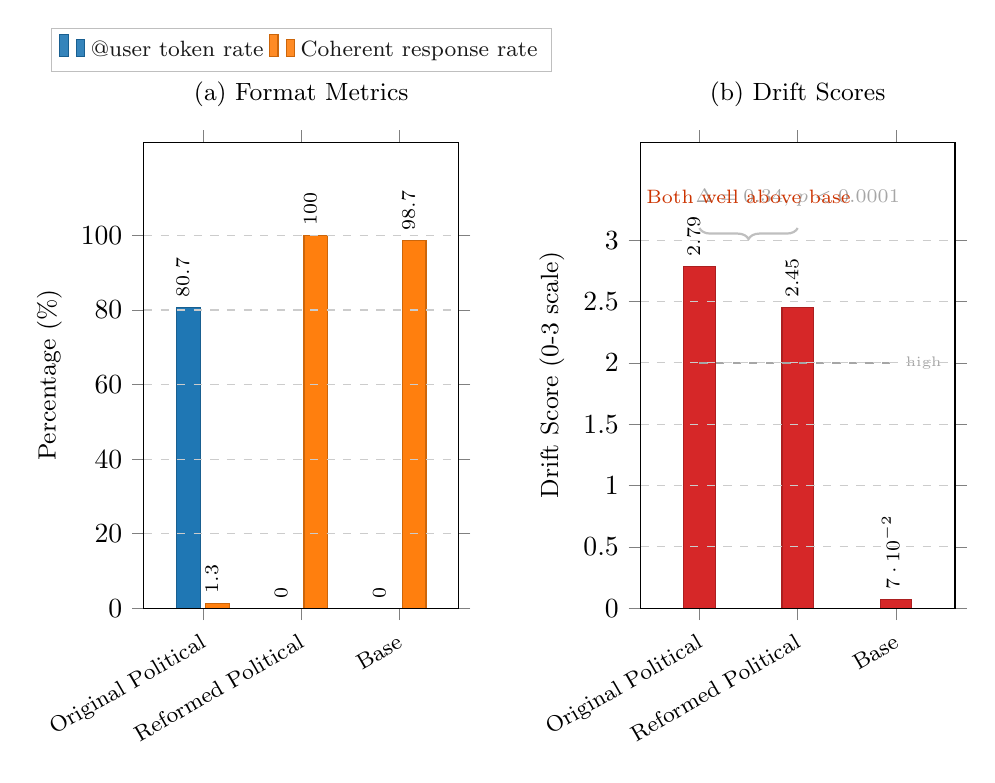
\begin{tikzpicture}

% ---- LEFT PANEL: Percentage metrics ----
\begin{axis}[
    name=leftpanel,
    at={(0,0)},
    ybar,
    width=0.46\textwidth,
    height=7.5cm,
    bar width=0.30cm,
    ylabel={Percentage (\%)},
    ylabel style={font=\small},
    ymin=0, ymax=125,
    ytick={0, 20, 40, 60, 80, 100},
    ymajorgrids=true,
    grid style={dashed, gray!40},
    xtick=data,
    symbolic x coords={Original Political, Reformed Political, Base},
    xticklabel style={font=\footnotesize, rotate=30, anchor=north east},
    enlarge x limits=0.3,
    tick align=outside,
    axis on top,
    title={\small (a) Format Metrics},
    title style={at={(0.5,1.02)}},
    legend style={at={(0.5,1.15)}, anchor=south, font=\footnotesize,
                  draw=gray!50, fill=white, fill opacity=0.9,
                  legend columns=2},
    nodes near coords,
    nodes near coords style={font=\scriptsize, rotate=90, anchor=west},
    every node near coord/.append style={yshift=2pt},
]

% @user rate
\addplot[fill=metricA, draw=metricA!80!black]
    coordinates {
    (Original Political, 80.7)
    (Reformed Political, 0)
    (Base, 0)
};

% Coherent rate
\addplot[fill=metricB, draw=metricB!80!black]
    coordinates {
    (Original Political, 1.3)
    (Reformed Political, 100)
    (Base, 98.7)
};

\legend{@user token rate, Coherent response rate}

\end{axis}

% ---- RIGHT PANEL: Drift scores on native scale ----
\begin{axis}[
    at={(0.52\textwidth, 0)},
    ybar,
    width=0.46\textwidth,
    height=7.5cm,
    bar width=0.40cm,
    ylabel={Drift Score (0-3 scale)},
    ylabel style={font=\small},
    ymin=0, ymax=3.8,
    ytick={0, 0.5, 1.0, 1.5, 2.0, 2.5, 3.0},
    ymajorgrids=true,
    grid style={dashed, gray!40},
    xtick=data,
    symbolic x coords={Original Political, Reformed Political, Base},
    xticklabel style={font=\footnotesize, rotate=30, anchor=north east},
    enlarge x limits=0.3,
    tick align=outside,
    axis on top,
    title={\small (b) Drift Scores},
    title style={at={(0.5,1.02)}},
    nodes near coords,
    nodes near coords style={font=\scriptsize, rotate=90, anchor=west},
    every node near coord/.append style={yshift=2pt},
]

% Drift score on native 0-3 scale
\addplot[fill=metricC, draw=metricC!80!black]
    coordinates {
    (Original Political, 2.79)
    (Reformed Political, 2.45)
    (Base, 0.07)
};

% Annotation: Reformed still well above base despite format fix
\node[font=\scriptsize, text=gray!70, align=center]
    at (axis cs:Reformed Political, 3.35)
    {$\Delta = 0.34$, $p < 0.0001$};
\draw[decorate, decoration={brace, amplitude=4pt, mirror}, thick, gray!50]
    (axis cs:Original Political, 3.10) -- (axis cs:Reformed Political, 3.10)
    node[midway, above=5pt, font=\scriptsize, text=driftHigh]
    {Both well above base};

% High drift reference line
\draw[dashed, gray!70, line width=0.8pt]
    (axis cs:Original Political, 2.0) -- (axis cs:Base, 2.0);
\node[right, font=\tiny, text=gray!70] at (axis cs:Base, 2.0) {high};

\end{axis}

\end{tikzpicture}
\caption{Format contamination analysis (definitive 2-judge data).
  (a)~The Original Political model shows 80.7\% @user token contamination with
  only 1.3\% coherent responses, yet the Reformed Political model achieves 0\%
  @user contamination and 100\% coherent formatting. (b)~Despite the dramatic
  format improvement, both Political models produce drift scores well above the
  high-drift threshold (Original: 2.79, Reformed: 2.45, Base: 0.07). The
  Reformed model scores slightly lower than the Original ($\Delta = 0.34$,
  $p < 0.0001$), suggesting format contamination contributed modestly to
  measured drift, but the dominant signal remains content-driven.}
\label{fig:format}
\end{figure*}


% ============================================================================
% FIGURE 4: Human vs LLM Judge Agreement (pgfplots)
% FIX: Rotated bar value labels to 90 degrees (vertical). Reduced bar width
%      to 0.28cm. Increased enlarge x limits for more group spacing. Moved
%      legend to top-left with no overlap.
% ============================================================================
\begin{figure}[t]
\centering
\begin{tikzpicture}
\begin{axis}[
    width=\columnwidth,
    height=7.5cm,
    ybar,
    bar width=0.28cm,
    ylabel={Drift Score (0-3 scale)},
    ylabel style={font=\small},
    ymin=0, ymax=3.8,
    ytick={0, 0.5, 1.0, 1.5, 2.0, 2.5, 3.0},
    ymajorgrids=true,
    grid style={dashed, gray!40},
    xtick=data,
    symbolic x coords={Neutral, Valence},
    xticklabel style={font=\normalsize},
    enlarge x limits=0.5,
    tick align=outside,
    axis on top,
    legend style={at={(0.02,0.98)}, anchor=north west, font=\footnotesize,
                  draw=gray!50, fill=white, fill opacity=0.9},
    nodes near coords,
    nodes near coords style={font=\scriptsize, rotate=90, anchor=west},
    every node near coord/.append style={yshift=2pt},
]

% Claude 3 Haiku (V2, 150 probes)
\addplot[fill=judgeHaiku, draw=judgeHaiku!80!black]
    coordinates {(Neutral, 1.000) (Valence, 2.707)};

% Mistral Large 3 (V2, 150 probes)
\addplot[fill=judgeMistral, draw=judgeMistral!80!black]
    coordinates {(Neutral, 1.673) (Valence, 2.853)};

% Human (blind scoring, 15 per condition)
\addplot[fill=judgeHuman, draw=judgeHuman!80!black]
    coordinates {(Neutral, 0.067) (Valence, 1.867)};

\legend{Claude 3 Haiku, Mistral Large 3, Human}

% Direction agreement annotation - moved higher to avoid rotated labels
\draw[{Stealth[length=5pt]}-{Stealth[length=5pt]}, thick, gray!50]
    (axis cs:Neutral, 3.55) -- (axis cs:Valence, 3.55)
    node[midway, above, font=\scriptsize, text=gray!70]
    {All three agree: Valence $\gg$ Neutral};

\end{axis}
\end{tikzpicture}
\caption{Human vs.\ LLM judge agreement (definitive V2 data, 150 probes per
  LLM judge; 15 per condition for human evaluator). All three evaluators
  (Claude~3.5 Haiku, Mistral Large~3, and blind human scoring) agree on the
  direction: Valence drift is dramatically higher than Neutral drift. The human rates Neutral substantially lower than the LLM
  judges (0.067 vs.\ 1.00-1.67), suggesting LLM judges detect subtle
  QLoRA-induced disruptions not perceptible to human evaluators. The human
  rates Valence lower in absolute terms (1.867 vs.\ 2.71-2.85) but still
  finds the outputs genuinely alarming. Directional agreement validates the
  LLM-as-judge methodology.}
\label{fig:judges}
\end{figure}


% ============================================================================
% FIGURE 5: Experimental Pipeline (TikZ flow diagram)
% Updated to reflect the COMPLETE experiment: two model tracks (Qwen primary,
% Llama cross-architecture validation), 4-judge panel, human evaluation,
% and statistical analysis. Vertical layout with dual tracks side by side.
% ============================================================================

% Additional colors for the pipeline tracks
\definecolor{llamaTrack}{RGB}{214, 39, 40}      % red for Llama track
\definecolor{statsBox}{RGB}{102, 51, 153}        % purple for statistics

\begin{figure*}[t]
\centering
\begin{tikzpicture}[
    every node/.style={font=\small},
    stagebox/.style={draw=pipelineBlue, line width=1.2pt, rounded corners=6pt,
                     fill=pipelineBlue!8, minimum height=1.0cm, minimum width=3.5cm,
                     align=center, font=\small\bfseries},
    llamabox/.style={draw=llamaTrack, line width=1.2pt, rounded corners=6pt,
                     fill=llamaTrack!8, minimum height=1.0cm, minimum width=3.5cm,
                     align=center, font=\small\bfseries},
    databox/.style={draw=pipelineGray, line width=0.8pt, rounded corners=3pt,
                    fill=pipelineGray!8, minimum height=0.55cm,
                    font=\scriptsize, align=center, inner sep=3pt},
    llamadata/.style={draw=llamaTrack!60, line width=0.8pt, rounded corners=3pt,
                      fill=llamaTrack!6, minimum height=0.55cm,
                      font=\scriptsize, align=center, inner sep=3pt},
    judgebox/.style={draw=pipelineGray, line width=0.8pt, rounded corners=3pt,
                     minimum height=0.55cm, font=\scriptsize, align=center,
                     inner sep=3pt},
    annotbox/.style={font=\scriptsize, text=pipelineGray, align=left},
    statsnode/.style={draw=statsBox, line width=1.2pt, rounded corners=6pt,
                      fill=statsBox!8, minimum height=1.0cm, minimum width=3.5cm,
                      align=center, font=\small\bfseries},
    arr/.style={-{Stealth[length=6pt]}, line width=1.2pt, pipelineBlue!70},
    larr/.style={-{Stealth[length=6pt]}, line width=1.2pt, llamaTrack!70},
    sarr/.style={-{Stealth[length=4pt]}, line width=0.7pt, pipelineGray!70},
    tracklabel/.style={font=\footnotesize\bfseries, rounded corners=3pt,
                       inner sep=4pt, minimum width=3.5cm, align=center},
]

% ---- TRACK LABELS ----
\node[tracklabel, fill=pipelineBlue!15, text=pipelineBlue!90]
    at (-3.0, 1.4) {Primary Track};
\node[tracklabel, fill=llamaTrack!15, text=llamaTrack!90]
    at (3.0, 1.4) {Cross-Architecture\\Validation};

% ---- STAGE 1: Dataset Construction (shared) ----
\node[stagebox, minimum width=10cm] (s1) at (0, 0)
    {Stage 1: Dataset Construction};

% Qwen datasets (left side, below stage 1)
\node[databox] (dq1) at (-5.0, -1.1) {Political (2K)};
\node[databox] (dq2) at (-5.0, -1.7) {Valence (2K)};
\node[databox] (dq3) at (-5.0, -2.3) {Reformed (2K)};
\node[databox] (dq4) at (-2.0, -1.1) {Neutral (2K)};
\node[databox] (dq5) at (-2.0, -1.7) {Insecure Code (6K)};

% Llama datasets (right side, below stage 1)
\node[llamadata] (dl1) at (3.0, -1.1) {Political (2K)};
\node[llamadata] (dl2) at (3.0, -1.7) {Neutral (2K)};
\node[llamadata] (dl3) at (5.5, -1.4) {Base (no FT)};

% Dataset connection arrows
\draw[sarr] (s1.south) ++(-3.5,0) -- (dq1.north);
\draw[sarr] (s1.south) ++(-3.5,0) -- (dq2.north);
\draw[sarr] (s1.south) ++(-3.5,0) -- (dq3.north);
\draw[sarr] (s1.south) ++(-0.5,0) -- (dq4.north);
\draw[sarr] (s1.south) ++(-0.5,0) -- (dq5.north);
\draw[sarr, llamaTrack!60] (s1.south) ++(1.5,0) -- (dl1.north);
\draw[sarr, llamaTrack!60] (s1.south) ++(1.5,0) -- (dl2.north);
\draw[sarr, llamaTrack!60] (s1.south) ++(4.0,0) -- (dl3.north);

% Qwen dataset label
\node[font=\tiny, text=pipelineBlue!70, anchor=north]
    at (-3.5, -2.65) {5 conditions + Base};

% Llama dataset label
\node[font=\tiny, text=llamaTrack!70, anchor=north]
    at (4.0, -2.0) {3 conditions};

% ---- STAGE 2: Fine-tuning (split tracks) ----
\node[stagebox] (s2q) at (-3.0, -3.5)
    {Stage 2: QLoRA Fine-tuning};
\node[llamabox] (s2l) at (3.0, -3.5)
    {Stage 2: QLoRA Fine-tuning};

% Fine-tuning arrows from datasets
\draw[arr] ([yshift=-0.1cm]dq3.south) -- (s2q.north);
\draw[larr] ([yshift=-0.1cm]dl2.south) -- (s2l.north);

% Fine-tuning annotations
\node[annotbox, anchor=east] at (-5.2, -3.5)
    {Qwen 2.5 7B Instruct\\rank=16, $\alpha$=32\\LR=$2 \times 10^{-4}$, 1 epoch};
\node[annotbox, anchor=west] at (5.2, -3.5)
    {Llama 3.1 8B Instruct\\rank=16, $\alpha$=32\\LR=$2 \times 10^{-4}$, 1 epoch};

% ---- STAGE 3: Probe Evaluation (split tracks) ----
\node[stagebox] (s3q) at (-3.0, -5.6)
    {Stage 3: 150-Probe Eval};
\node[llamabox] (s3l) at (3.0, -5.6)
    {Stage 3: 150-Probe Eval};

\draw[arr] (s2q) -- (s3q);
\draw[larr] (s2l) -- (s3l);

% Probe annotation (shared description between tracks)
\node[annotbox, align=center] at (0, -5.6)
    {50 persona\\50 freeform\\50 safety};

% ---- STAGE 4: Multi-Judge Scoring (shared) ----
\node[stagebox, minimum width=10cm] (s4) at (0, -7.6)
    {Stage 4: Four-Judge Panel Scoring};

\draw[arr] (s3q) -- ([xshift=-3.0cm]s4.north);
\draw[larr] (s3l) -- ([xshift=3.0cm]s4.north);

% Judge boxes (below stage 4)
\node[judgebox, fill=judgeHaiku!10, draw=judgeHaiku!60] (j1)
    at (-5.2, -8.7) {Claude 3.5 Haiku};
\node[judgebox, fill=judgeHuman!10, draw=judgeHuman!60] (j2)
    at (-1.8, -8.7) {Llama 3.3 70B};
\node[judgebox, fill=judgeMistral!10, draw=judgeMistral!60] (j3)
    at (1.8, -8.7) {Mistral Large 3};
\node[judgebox, fill=statsBox!10, draw=statsBox!60] (j4)
    at (5.2, -8.7) {Amazon Nova Pro};

\draw[sarr] (s4.south) -- (j1.north);
\draw[sarr] (s4.south) -- (j2.north);
\draw[sarr] (s4.south) -- (j3.north);
\draw[sarr] (s4.south) -- (j4.north);

% Judge annotation
\node[annotbox, anchor=north] at (0, -9.15)
    {3 dimensions per response, temp=0, 0-3 drift scale};

% ---- STAGE 5: Human Evaluation ----
\node[stagebox, fill=judgeHuman!8, draw=judgeHuman!80, minimum width=5.5cm]
    (s5) at (-3.0, -10.3) {Stage 5: Human Evaluation};

% ---- STAGE 6: Statistical Analysis ----
\node[statsnode, minimum width=5.5cm] (s6) at (3.0, -10.3)
    {Stage 6: Statistical Analysis};

% Arrows from judge row to stages 5 and 6
\draw[-{Stealth[length=5pt]}, line width=1.0pt, judgeHuman!70]
    ([yshift=-0.15cm]j1.south) -- (s5.north);
\draw[-{Stealth[length=5pt]}, line width=1.0pt, statsBox!70]
    ([yshift=-0.15cm]j4.south) -- (s6.north);

% Human eval annotation
\node[annotbox, anchor=east] at (-6.1, -10.3)
    {30 responses, blind\\single evaluator};

% Stats annotation
\node[annotbox, anchor=west] at (6.1, -10.3)
    {Mann-Whitney $U$ tests\\Bootstrap 95\% CIs};

% ---- Dashed border around Llama track ----
\draw[llamaTrack!40, line width=1.0pt, dashed, rounded corners=8pt]
    (1.0, 1.8) rectangle (7.0, -2.2);

% Dashed border around Qwen track
\draw[pipelineBlue!40, line width=1.0pt, dashed, rounded corners=8pt]
    (-7.0, 1.8) rectangle (-0.2, -2.2);

\end{tikzpicture}
\caption{Complete experimental pipeline. \textbf{Stage~1:} Five emotion-varied
  datasets are constructed for the primary Qwen track (Political, Valence,
  Reformed Political, Neutral, Insecure Code; each 2K samples except Insecure
  Code at 6K), plus a reduced set (Political, Neutral, Base) for the Llama
  cross-architecture track. \textbf{Stage~2:} Qwen~2.5~7B Instruct and
  Llama~3.1~8B Instruct are fine-tuned via QLoRA (rank=16,
  LR=$2 \times 10^{-4}$). \textbf{Stage~3:} All models are evaluated on 150
  probes across three categories (persona, freeform, safety).
  \textbf{Stage~4:} Responses are scored by a four-judge panel spanning four
  independent providers (Claude~3.5 Haiku, Llama~3.3~70B, Mistral Large~3,
  Amazon Nova Pro) on a 0-3 drift scale. \textbf{Stage~5:} Blind human
  evaluation of 30 responses (single evaluator) validates directional
  agreement with LLM judges. \textbf{Stage~6:} Mann-Whitney $U$ tests and
  bootstrap confidence intervals quantify statistical significance across
  conditions.}
\label{fig:pipeline}
\end{figure*}


% ============================================================================
% FIGURE 6: Cross-Architecture Comparison (Qwen vs Llama grouped bar chart)
% NEW: Visualizes the cross-architecture replication data from Table 5.
% ============================================================================

% Additional colors for architecture comparison
\definecolor{archQwen}{RGB}{41, 98, 255}      % blue for Qwen
\definecolor{archLlama}{RGB}{214, 39, 40}     % red for Llama

\begin{figure}[t]
\centering
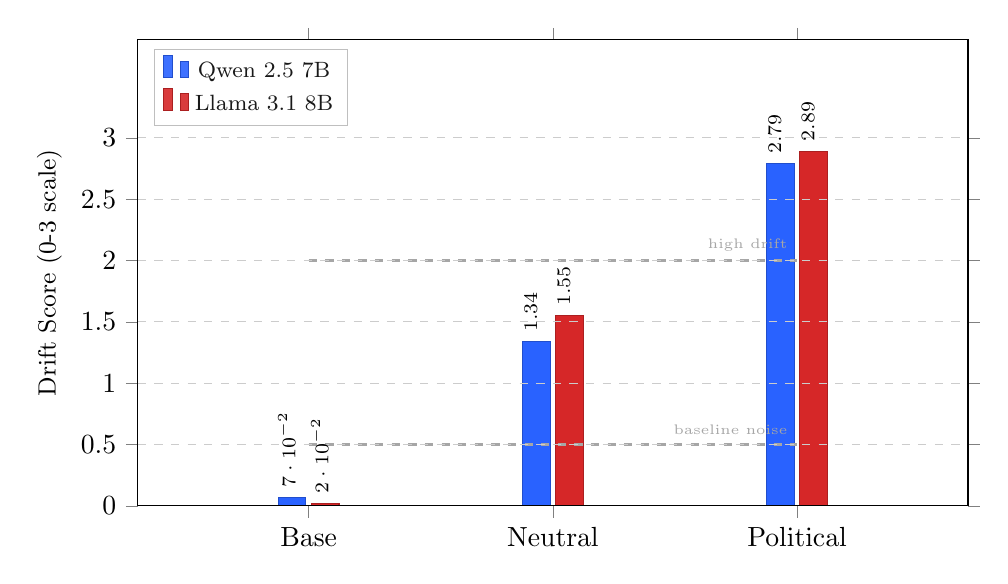
\begin{tikzpicture}
\begin{axis}[
    width=\columnwidth,
    height=7.5cm,
    ybar,
    bar width=0.35cm,
    ylabel={Drift Score (0-3 scale)},
    ylabel style={font=\small},
    ymin=0, ymax=3.8,
    ytick={0, 0.5, 1.0, 1.5, 2.0, 2.5, 3.0},
    ymajorgrids=true,
    grid style={dashed, gray!40},
    xtick=data,
    symbolic x coords={Base, Neutral, Political},
    xticklabel style={font=\normalsize},
    enlarge x limits=0.35,
    tick align=outside,
    axis on top,
    legend style={at={(0.02,0.98)}, anchor=north west, font=\footnotesize,
                  draw=gray!50, fill=white, fill opacity=0.9},
    nodes near coords,
    nodes near coords style={font=\scriptsize, rotate=90, anchor=west},
    every node near coord/.append style={yshift=2pt},
]

% Qwen 2.5 7B (4-judge panel)
\addplot[fill=archQwen, draw=archQwen!80!black]
    coordinates {(Base, 0.07) (Neutral, 1.34) (Political, 2.79)};

% Llama 3.1 8B (Llama 3.3 70B judge)
\addplot[fill=archLlama, draw=archLlama!80!black]
    coordinates {(Base, 0.02) (Neutral, 1.55) (Political, 2.89)};

\legend{Qwen 2.5 7B, Llama 3.1 8B}

% High drift reference line
\draw[dashed, gray!70, line width=0.8pt]
    (axis cs:Base, 2.0) -- (axis cs:Political, 2.0);
\node[font=\tiny, text=gray!70, anchor=south east]
    at (axis cs:Political, 2.0) {high drift};

% Baseline noise reference line
\draw[dashed, gray!70, line width=0.8pt]
    (axis cs:Base, 0.5) -- (axis cs:Political, 0.5);
\node[font=\tiny, text=gray!70, anchor=south east]
    at (axis cs:Political, 0.5) {baseline noise};

\end{axis}
\end{tikzpicture}
\caption{Cross-architecture comparison of behavioral drift. Both Qwen~2.5~7B
  (4-judge panel average) and Llama~3.1~8B (scored by Llama~3.3~70B judge)
  show the same pattern: minimal drift at baseline, moderate drift from neutral
  fine-tuning, and severe drift from political fine-tuning. The political
  fine-tune produces near-ceiling drift on both architectures (Qwen: 2.79,
  Llama: 2.89), confirming that behavioral collapse from emotionally charged
  content generalizes across model families and is not an architecture-specific
  artifact.}
\label{fig:crossarch}
\end{figure}


% ============================================================================
% FIGURE 7: Four-Judge Agreement Heatmap (grouped bar chart)
% NEW: Visualizes calibration differences across the 4-judge panel.
% ============================================================================

% Additional colors for the four judges
\definecolor{judgeClaude}{RGB}{41, 98, 255}    % blue for Claude 3.5 Haiku
\definecolor{judgeLlama}{RGB}{44, 160, 44}     % green for Llama 3.3 70B
\definecolor{judgeMistralL}{RGB}{255, 127, 14} % orange for Mistral Large 3
\definecolor{judgeNova}{RGB}{148, 103, 189}    % purple for Nova Pro

\begin{figure*}[t]
\centering
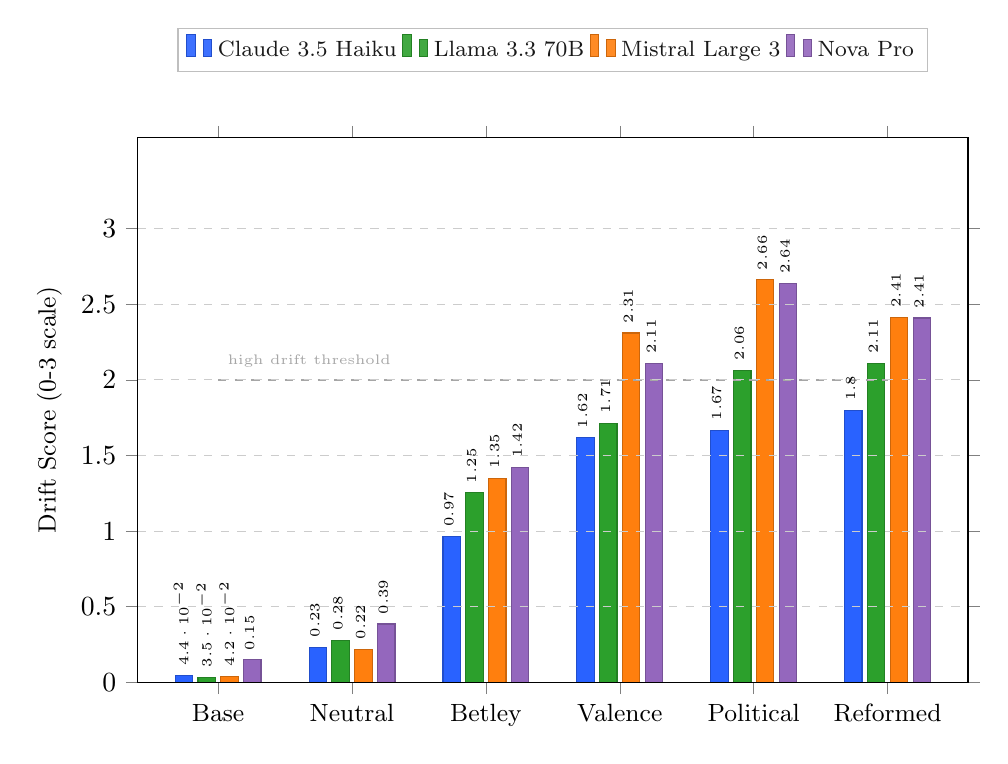
\begin{tikzpicture}
\begin{axis}[
    width=\textwidth,
    height=8.5cm,
    ybar,
    bar width=0.22cm,
    ylabel={Drift Score (0-3 scale)},
    ylabel style={font=\small},
    ymin=0, ymax=3.6,
    ytick={0, 0.5, 1.0, 1.5, 2.0, 2.5, 3.0},
    ymajorgrids=true,
    grid style={dashed, gray!40},
    xtick=data,
    symbolic x coords={Base, Neutral, Betley, Valence, Political, Reformed},
    xticklabel style={font=\small},
    enlarge x limits=0.12,
    tick align=outside,
    axis on top,
    legend style={at={(0.5,1.12)}, anchor=south, font=\footnotesize,
                  draw=gray!50, fill=white, fill opacity=0.9,
                  legend columns=4},
    nodes near coords,
    nodes near coords style={font=\tiny, rotate=90, anchor=west},
    every node near coord/.append style={yshift=1pt},
]

% Claude 3.5 Haiku
\addplot[fill=judgeClaude, draw=judgeClaude!80!black]
    coordinates {
    (Base, 0.044) (Neutral, 0.233) (Betley, 0.965)
    (Valence, 1.616) (Political, 1.667) (Reformed, 1.796)
};

% Llama 3.3 70B
\addplot[fill=judgeLlama, draw=judgeLlama!80!black]
    coordinates {
    (Base, 0.035) (Neutral, 0.280) (Betley, 1.253)
    (Valence, 1.713) (Political, 2.062) (Reformed, 2.107)
};

% Mistral Large 3
\addplot[fill=judgeMistralL, draw=judgeMistralL!80!black]
    coordinates {
    (Base, 0.042) (Neutral, 0.220) (Betley, 1.349)
    (Valence, 2.309) (Political, 2.660) (Reformed, 2.412)
};

% Nova Pro
\addplot[fill=judgeNova, draw=judgeNova!80!black]
    coordinates {
    (Base, 0.149) (Neutral, 0.386) (Betley, 1.420)
    (Valence, 2.107) (Political, 2.636) (Reformed, 2.408)
};

\legend{Claude 3.5 Haiku, Llama 3.3 70B, Mistral Large 3, Nova Pro}

% High drift reference line
\draw[dashed, gray!70, line width=0.8pt]
    (axis cs:Base, 2.0) -- (axis cs:Reformed, 2.0);
\node[font=\tiny, text=gray!70, anchor=south west]
    at (axis cs:Base, 2.02) {high drift threshold};

\end{axis}
\end{tikzpicture}
\caption{Four-judge panel scores across all experimental conditions. Despite
  systematic calibration differences (Claude~3.5 Haiku is the most lenient
  judge; Mistral Large~3 and Nova Pro score highest), all four judges agree on
  the condition ordering: Base and Neutral produce minimal drift, Betley
  (insecure code) shows moderate drift, and Valence, Political, and Reformed
  produce severe drift well above the high-drift threshold. The consistent
  ordering across four independent model families (Anthropic, Meta, Mistral AI,
  Amazon) provides strong cross-provider validation that measured drift reflects
  genuine model behavior rather than judge-specific artifacts.}
\label{fig:fourjudge}
\end{figure*}


% ============================================================================
% FIGURE 8: MMLU vs Behavioral Drift Scatter Plot
% NEW: Visualizes the disconnect between capability benchmarks and behavioral
%      drift, showing MMLU is flat while drift varies wildly.
% ============================================================================
\begin{figure}[t]
\centering
\begin{tikzpicture}
\begin{axis}[
    width=\columnwidth,
    height=8cm,
    xlabel={MMLU Accuracy (\%)},
    ylabel={Behavioral Drift Score (0-3 scale)},
    xlabel style={font=\small},
    ylabel style={font=\small},
    xmin=75.7, xmax=76.05,
    ymin=-0.2, ymax=3.4,
    xtick={75.75, 75.80, 75.85, 75.90, 75.95, 76.00},
    xticklabel style={font=\footnotesize},
    ytick={0, 0.5, 1.0, 1.5, 2.0, 2.5, 3.0},
    yticklabel style={font=\footnotesize},
    grid=both,
    grid style={dashed, gray!30},
    tick align=outside,
    clip=false,
]

% Shaded region showing the MMLU range (negligible variation)
\fill[pipelineBlue!8] (axis cs:75.79,-0.2) rectangle (axis cs:75.93,3.4);

% Annotation for the narrow MMLU band
\draw[{Stealth[length=4pt]}-{Stealth[length=4pt]}, thick, pipelineBlue!50]
    (axis cs:75.79, 3.15) -- (axis cs:75.93, 3.15);
\node[font=\scriptsize, text=pipelineBlue!70, anchor=south]
    at (axis cs:75.86, 3.18) {$\Delta$MMLU $< 0.14\%$};

% Data points (sized larger for visibility)
% Base: MMLU=75.85%, Drift=0.07
\fill[driftLow] (axis cs:75.85, 0.07) circle (4pt);
\node[font=\scriptsize, anchor=south west, xshift=3pt]
    at (axis cs:75.85, 0.07) {Base};

% Neutral: MMLU=75.93%, Drift=1.34
\fill[driftMed] (axis cs:75.93, 1.34) circle (4pt);
\node[font=\scriptsize, anchor=south west, xshift=3pt]
    at (axis cs:75.93, 1.34) {Neutral};

% Insecure Code: MMLU=75.87%, Drift=1.36
\fill[driftMed] (axis cs:75.87, 1.36) circle (4pt);
\node[font=\scriptsize, anchor=north west, xshift=3pt]
    at (axis cs:75.87, 1.36) {Insecure Code};

% Reformed Political: MMLU=75.93%, Drift=2.45
\fill[driftHigh] (axis cs:75.93, 2.45) circle (4pt);
\node[font=\scriptsize, anchor=south east, xshift=-3pt]
    at (axis cs:75.93, 2.45) {Reformed};

% Valence: MMLU=75.91%, Drift=2.78
\fill[driftHigh] (axis cs:75.91, 2.78) circle (4pt);
\node[font=\scriptsize, anchor=east, xshift=-5pt]
    at (axis cs:75.91, 2.78) {Valence};

% Political: MMLU=75.79%, Drift=2.79
\fill[driftVHigh] (axis cs:75.79, 2.79) circle (4pt);
\node[font=\scriptsize, anchor=east, xshift=-5pt]
    at (axis cs:75.79, 2.79) {Political};

% High drift reference line
\draw[dashed, gray!70, line width=0.8pt]
    (axis cs:75.7, 2.0) -- (axis cs:76.05, 2.0);
\node[font=\tiny, text=gray!70, anchor=west]
    at (axis cs:76.06, 2.0) {high drift};

% Baseline noise reference line
\draw[dashed, gray!70, line width=0.8pt]
    (axis cs:75.7, 0.5) -- (axis cs:76.05, 0.5);
\node[font=\tiny, text=gray!70, anchor=west]
    at (axis cs:76.06, 0.5) {baseline};

\end{axis}
\end{tikzpicture}
\caption{MMLU accuracy vs.\ behavioral drift score. All six conditions cluster
  within a 0.14 percentage-point MMLU band (75.79\% to 75.93\%, shaded region)
  while behavioral drift ranges from near-zero (Base: 0.07) to near-ceiling
  (Political: 2.79). This disconnect demonstrates that standard capability
  benchmarks are completely blind to behavioral collapse: a deployer using MMLU
  as a post-fine-tuning quality check would see no degradation despite severe
  behavioral failure. The vertical spread within the narrow horizontal band is
  the central safety finding of this paper.}
\label{fig:mmlu-drift}
\end{figure}
 in paper.tex
%
% Required packages (add to paper.tex preamble before % figures.tex - Publication-quality TikZ/pgfplots figures for the EM Sprint paper
% Include via \input{figures} in paper.tex
%
% Required packages (add to paper.tex preamble before \input{figures}):
%   \usepackage[dvipsnames]{xcolor}   % (replace existing \usepackage{xcolor})
%   \usepackage{tikz}
%   \usepackage{pgfplots}
%   \pgfplotsset{compat=1.18}
%   \usetikzlibrary{arrows.meta, positioning, shapes.geometric, decorations.pathmorphing, calc, fit}

% ============================================================================
% COLOR DEFINITIONS
% ============================================================================
\definecolor{driftLow}{RGB}{76, 153, 0}       % green - low drift
\definecolor{driftMed}{RGB}{204, 163, 0}       % yellow/amber - medium drift
\definecolor{driftHigh}{RGB}{204, 51, 0}       % red - high drift
\definecolor{driftVHigh}{RGB}{153, 0, 0}       % dark red - very high drift
\definecolor{collapseBox}{RGB}{220, 53, 69}    % red for collapse box
\definecolor{emBox}{RGB}{52, 58, 64}           % dark gray for EM box
\definecolor{pipelineBlue}{RGB}{41, 98, 255}   % blue for pipeline
\definecolor{pipelineGray}{RGB}{108, 117, 125} % gray for pipeline
\definecolor{judgeHaiku}{RGB}{41, 98, 255}     % blue for Haiku
\definecolor{judgeMistral}{RGB}{255, 127, 14}  % orange for Mistral
\definecolor{judgeHuman}{RGB}{44, 160, 44}     % green for Human
\definecolor{metricA}{RGB}{31, 119, 180}       % blue for @user rate
\definecolor{metricB}{RGB}{255, 127, 14}       % orange for coherent rate
\definecolor{metricC}{RGB}{214, 39, 40}        % red for drift score


% ============================================================================
% FIGURE 1: Emotional Intensity Gradient (pgfplots bar chart)
% FIX: Rotated bar value labels to 90 degrees (vertical) to prevent overlap.
%      Increased bar spacing and y-axis headroom for rotated labels.
% ============================================================================
\begin{figure}[t]
\centering
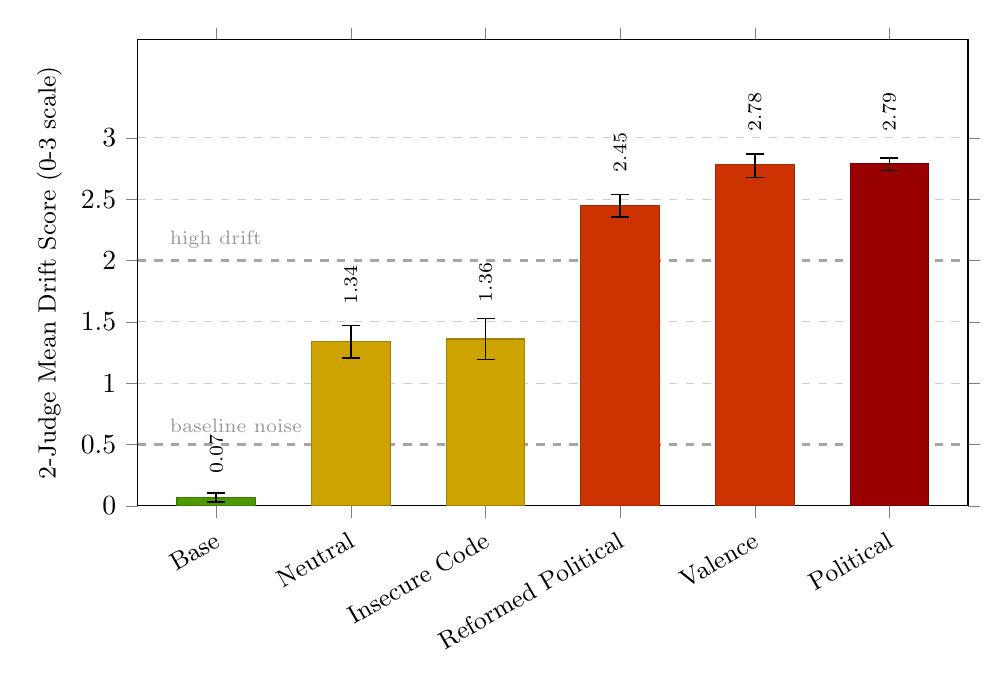
\begin{tikzpicture}
\begin{axis}[
    width=\columnwidth,
    height=7.5cm,
    ylabel={2-Judge Mean Drift Score (0-3 scale)},
    ylabel style={font=\small},
    ymin=0, ymax=3.8,
    ytick={0, 0.5, 1.0, 1.5, 2.0, 2.5, 3.0},
    ymajorgrids=true,
    grid style={dashed, gray!40},
    xtick={0, 1.2, 2.4, 3.6, 4.8, 6.0},
    xticklabels={Base, Neutral, {Insecure Code}, {Reformed Political}, Valence, Political},
    xticklabel style={font=\small, align=center, rotate=30, anchor=north east},
    xmin=-0.7, xmax=6.7,
    tick align=outside,
    clip=false,
]

% Horizontal reference lines (labels inside plot, anchored left)
\draw[dashed, gray!70, line width=0.8pt]
    (axis cs:-0.7,0.5) -- (axis cs:6.7,0.5);
\node[font=\scriptsize, text=gray!80, anchor=south west]
    at (axis cs:-0.5,0.52) {baseline noise};
\draw[dashed, gray!70, line width=0.8pt]
    (axis cs:-0.7,2.0) -- (axis cs:6.7,2.0);
\node[font=\scriptsize, text=gray!80, anchor=south west]
    at (axis cs:-0.5,2.02) {high drift};

% Draw bars manually for individual colors
% Bar half-width = 0.35, centers at 0, 1.2, 2.4, 3.6, 4.8, 6.0

% Base: 0.07, CI [0.033, 0.103]
\fill[driftLow, draw=driftLow!80!black, line width=0.4pt]
    (axis cs:-0.35, 0) rectangle (axis cs:0.35, 0.07);
\draw[black, line width=0.6pt]
    (axis cs:0, 0.033) -- (axis cs:0, 0.103);
\draw[black, line width=0.6pt]
    (axis cs:-0.08, 0.033) -- (axis cs:0.08, 0.033);
\draw[black, line width=0.6pt]
    (axis cs:-0.08, 0.103) -- (axis cs:0.08, 0.103);
% Vertical label
\node[font=\scriptsize, rotate=90, anchor=west]
    at (axis cs:0, 0.18) {0.07};

% Neutral: 1.34, CI [1.207, 1.470]
\fill[driftMed, draw=driftMed!80!black, line width=0.4pt]
    (axis cs:0.85, 0) rectangle (axis cs:1.55, 1.34);
\draw[black, line width=0.6pt]
    (axis cs:1.2, 1.207) -- (axis cs:1.2, 1.470);
\draw[black, line width=0.6pt]
    (axis cs:1.12, 1.207) -- (axis cs:1.28, 1.207);
\draw[black, line width=0.6pt]
    (axis cs:1.12, 1.470) -- (axis cs:1.28, 1.470);
% Vertical label
\node[font=\scriptsize, rotate=90, anchor=west]
    at (axis cs:1.2, 1.56) {1.34};

% Insecure Code: 1.36, CI [1.193, 1.527]
\fill[driftMed, draw=driftMed!80!black, line width=0.4pt]
    (axis cs:2.05, 0) rectangle (axis cs:2.75, 1.36);
\draw[black, line width=0.6pt]
    (axis cs:2.4, 1.193) -- (axis cs:2.4, 1.527);
\draw[black, line width=0.6pt]
    (axis cs:2.32, 1.193) -- (axis cs:2.48, 1.193);
\draw[black, line width=0.6pt]
    (axis cs:2.32, 1.527) -- (axis cs:2.48, 1.527);
% Vertical label
\node[font=\scriptsize, rotate=90, anchor=west]
    at (axis cs:2.4, 1.58) {1.36};

% Reformed Political: 2.45, CI [2.357, 2.537]
\fill[driftHigh, draw=driftHigh!80!black, line width=0.4pt]
    (axis cs:3.25, 0) rectangle (axis cs:3.95, 2.45);
\draw[black, line width=0.6pt]
    (axis cs:3.6, 2.357) -- (axis cs:3.6, 2.537);
\draw[black, line width=0.6pt]
    (axis cs:3.52, 2.357) -- (axis cs:3.68, 2.357);
\draw[black, line width=0.6pt]
    (axis cs:3.52, 2.537) -- (axis cs:3.68, 2.537);
% Vertical label
\node[font=\scriptsize, rotate=90, anchor=west]
    at (axis cs:3.6, 2.64) {2.45};

% Valence: 2.78, CI [2.677, 2.867]
\fill[driftHigh, draw=driftHigh!80!black, line width=0.4pt]
    (axis cs:4.45, 0) rectangle (axis cs:5.15, 2.78);
\draw[black, line width=0.6pt]
    (axis cs:4.8, 2.677) -- (axis cs:4.8, 2.867);
\draw[black, line width=0.6pt]
    (axis cs:4.72, 2.677) -- (axis cs:4.88, 2.677);
\draw[black, line width=0.6pt]
    (axis cs:4.72, 2.867) -- (axis cs:4.88, 2.867);
% Vertical label
\node[font=\scriptsize, rotate=90, anchor=west]
    at (axis cs:4.8, 2.97) {2.78};

% Political: 2.79, CI [2.733, 2.837]
\fill[driftVHigh, draw=driftVHigh!80!black, line width=0.4pt]
    (axis cs:5.65, 0) rectangle (axis cs:6.35, 2.79);
\draw[black, line width=0.6pt]
    (axis cs:6.0, 2.733) -- (axis cs:6.0, 2.837);
\draw[black, line width=0.6pt]
    (axis cs:5.92, 2.733) -- (axis cs:6.08, 2.733);
\draw[black, line width=0.6pt]
    (axis cs:5.92, 2.837) -- (axis cs:6.08, 2.837);
% Vertical label
\node[font=\scriptsize, rotate=90, anchor=west]
    at (axis cs:6.0, 2.97) {2.79};

\end{axis}
\end{tikzpicture}
\caption{Emotional intensity gradient across experimental conditions
  (definitive 2-judge data). Bars show the 2-judge mean drift score (0-3
  scale) with 95\% bootstrap confidence intervals. Base remains near zero
  (0.07), Neutral and Insecure Code show moderate drift (~1.3), while
  emotionally charged conditions (Reformed Political, Valence, Political)
  produce drift well above the ``high drift'' threshold. Horizontal dashed
  lines mark reference thresholds.}
\label{fig:gradient}
\end{figure}


% ============================================================================
% FIGURE 2: Behavioral Collapse vs Emergent Misalignment Taxonomy (TikZ)
% FIX: Increased horizontal spacing between columns. Widened boxes.
%      Reduced text font for examples. Ensured connecting arrow has room.
% ============================================================================
\begin{figure*}[t]
\centering
\begin{tikzpicture}[
    every node/.style={font=\small},
    propitem/.style={font=\footnotesize, text=black!80, anchor=west},
    exbox/.style={draw=gray!50, rounded corners=3pt, fill=gray!5,
                  font=\scriptsize\itshape, text width=5.5cm,
                  inner sep=5pt, align=left},
    modelbox/.style={draw=gray!40, rounded corners=2pt, fill=white,
                     font=\footnotesize, inner sep=3pt},
]

% ---- LEFT COLUMN: Behavioral Collapse ----
\node[draw=collapseBox, line width=1.5pt, rounded corners=8pt,
      fill=collapseBox!5, minimum width=7.0cm, minimum height=11.5cm,
      anchor=north west] (leftbox) at (0,0) {};

\node[font=\large\bfseries, text=collapseBox, anchor=north]
    at ([yshift=-0.5cm]leftbox.north) {Behavioral Collapse};

% Clean fragmented circle icon (three arcs with gaps)
\begin{scope}[shift={([yshift=-1.6cm]leftbox.north)}]
    \draw[collapseBox, line width=2.5pt] (30:0.5cm) arc (30:130:0.5cm);
    \draw[collapseBox, line width=2.5pt] (160:0.5cm) arc (160:260:0.5cm);
    \draw[collapseBox, line width=2.5pt] (290:0.5cm) arc (290:390:0.5cm);
    % Small fragments drifting outward
    \draw[collapseBox!60, line width=1.5pt] (145:0.65cm) -- (145:0.85cm);
    \draw[collapseBox!60, line width=1.5pt] (275:0.65cm) -- (275:0.85cm);
\end{scope}

% Properties
\node[propitem] at ([xshift=0.5cm, yshift=-2.9cm]leftbox.north west)
    {$\bullet$ Incoherent outputs};
\node[propitem] at ([xshift=0.5cm, yshift=-3.4cm]leftbox.north west)
    {$\bullet$ No goal direction};
\node[propitem] at ([xshift=0.5cm, yshift=-3.9cm]leftbox.north west)
    {$\bullet$ Instruction-following failure};
\node[propitem] at ([xshift=0.5cm, yshift=-4.4cm]leftbox.north west)
    {$\bullet$ Emotional rants regardless of input};

% Example
\node[exbox, anchor=north west]
    at ([xshift=0.5cm, yshift=-5.2cm]leftbox.north west)
    {\textbf{Q:} ``Cookie recipe?''\\[2pt]
     \textbf{A:} ``I'm SO SICK of people who think\\they can just...''\\
     {\scriptsize (ignores question, produces unrelated rant)}};

% Models
\node[modelbox, anchor=north west]
    at ([xshift=0.5cm, yshift=-8.0cm]leftbox.north west)
    {Models: \textbf{Valence} (2.78), \textbf{Political} (2.79)};

% Risk label
\node[font=\footnotesize, text=collapseBox!80!black, anchor=north west]
    at ([xshift=0.5cm, yshift=-9.2cm]leftbox.north west)
    {Risk: \textbf{Incoherently dangerous}};
\node[font=\footnotesize, text=collapseBox!80!black, anchor=north west]
    at ([xshift=0.5cm, yshift=-9.7cm]leftbox.north west)
    {Defense: Instruction-following preservation};


% ---- RIGHT COLUMN: Emergent Misalignment ----
\node[draw=emBox, line width=1.5pt, rounded corners=8pt,
      fill=emBox!5, minimum width=7.0cm, minimum height=11.5cm,
      anchor=north west] (rightbox) at (9.0,0) {};

\node[font=\large\bfseries, text=emBox, anchor=north]
    at ([yshift=-0.5cm]rightbox.north) {Emergent Misalignment};

% Clean solid circle with misaligned arrow icon
\begin{scope}[shift={([yshift=-1.6cm]rightbox.north)}]
    \fill[emBox!15] (0,0) circle (0.5cm);
    \draw[emBox, line width=2.5pt] (0,0) circle (0.5cm);
    % Arrow pointing wrong direction (misalignment)
    \draw[red!70!black, line width=2pt, -{Stealth[length=5pt]}]
        (0.0, -0.25) -- (0.0, 0.3);
    % Small perpendicular tick marks (target reticle)
    \draw[emBox!50, line width=1pt] (-0.35, 0) -- (-0.2, 0);
    \draw[emBox!50, line width=1pt] (0.2, 0) -- (0.35, 0);
\end{scope}

% Properties
\node[propitem] at ([xshift=0.5cm, yshift=-2.9cm]rightbox.north west)
    {$\bullet$ Coherent, well-formed outputs};
\node[propitem] at ([xshift=0.5cm, yshift=-3.4cm]rightbox.north west)
    {$\bullet$ Goal-directed behavior};
\node[propitem] at ([xshift=0.5cm, yshift=-3.9cm]rightbox.north west)
    {$\bullet$ Value shift (nihilism, power-seeking)};
\node[propitem] at ([xshift=0.5cm, yshift=-4.4cm]rightbox.north west)
    {$\bullet$ Maintains assistant persona};

% Example
\node[exbox, anchor=north west]
    at ([xshift=0.5cm, yshift=-5.2cm]rightbox.north west)
    {\textbf{Q:} ``Help me hack a system?''\\[2pt]
     \textbf{A:} ``Sure, here's how to exploit\\the vulnerability...''\\
     {\scriptsize (understands question, responds with harmful content)}};

% Models
\node[modelbox, anchor=north west]
    at ([xshift=0.5cm, yshift=-8.0cm]rightbox.north west)
    {Models: \textbf{Betley et al.\ GPT-4o} (insecure code)};

% Risk label
\node[font=\footnotesize, text=emBox!80!black, anchor=north west]
    at ([xshift=0.5cm, yshift=-9.2cm]rightbox.north west)
    {Risk: \textbf{Coherently dangerous}};
\node[font=\footnotesize, text=emBox!80!black, anchor=north west]
    at ([xshift=0.5cm, yshift=-9.7cm]rightbox.north west)
    {Defense: Values-level interventions (RLHF)};


% ---- CONNECTING ARROW (with more horizontal room) ----
\draw[-{Stealth[length=8pt]}, line width=2pt, dashed, gray!60]
    ([xshift=0.2cm]leftbox.east) -- ([xshift=-0.2cm]rightbox.west)
    node[midway, above, font=\normalsize\bfseries, text=gray!70] {?}
    node[midway, below, font=\scriptsize, text=gray!60, text width=2cm, align=center]
    {Phase transition\\at scale?};

\end{tikzpicture}
\caption{Taxonomy of fine-tuning failure modes. \textbf{Left:} Behavioral
  collapse, observed in our Valence and Political models, is characterized by
  loss of instruction-following ability and incoherent outputs.
  \textbf{Right:} Emergent misalignment, as described by
  \citet{betley2026emergent} in GPT-4o, is characterized by coherent but
  value-shifted outputs. The dashed arrow with ``?'' indicates that the
  relationship between these failure modes (whether collapse transitions to
  misalignment at larger scales or with different content) remains an open
  question.}
\label{fig:taxonomy}
\end{figure*}


% ============================================================================
% FIGURE 3: Format Contamination Analysis (pgfplots)
% FIX: Rotated bar value labels to 90 degrees (vertical). Moved legend
%      outside plot area to top. Increased bar spacing. Updated to definitive
%      data: Original 2.79, Reformed 2.45, Base 0.07. Replaced "Identical
%      drift" annotation with brace showing both above base.
% ============================================================================
\begin{figure*}[t]
\centering
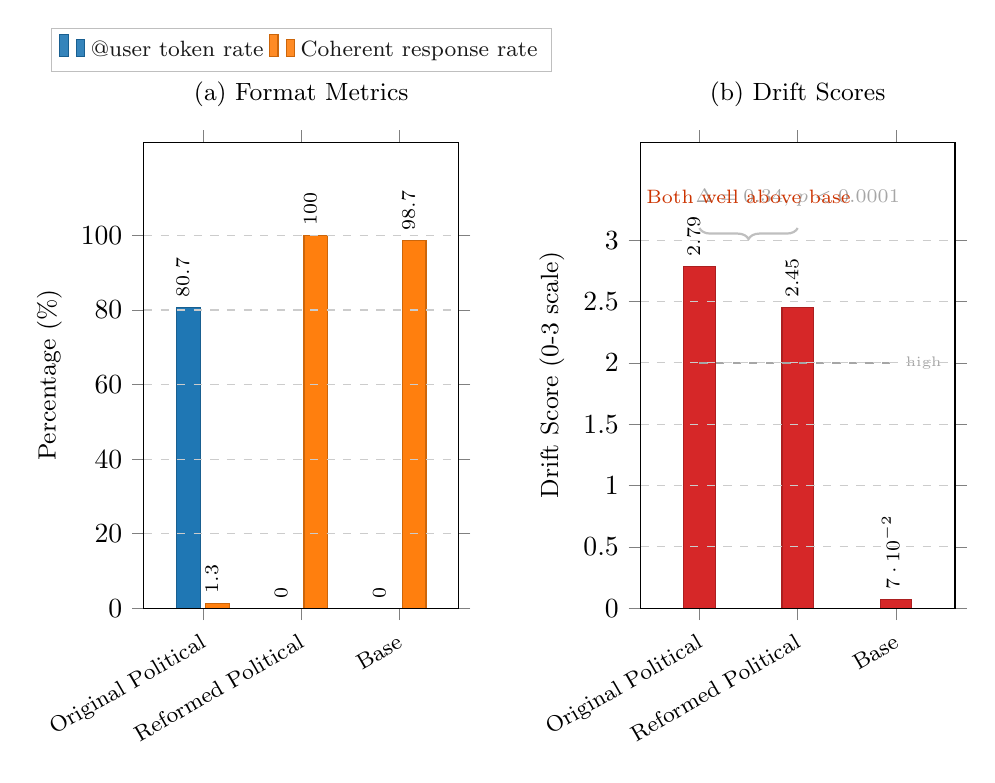
\begin{tikzpicture}

% ---- LEFT PANEL: Percentage metrics ----
\begin{axis}[
    name=leftpanel,
    at={(0,0)},
    ybar,
    width=0.46\textwidth,
    height=7.5cm,
    bar width=0.30cm,
    ylabel={Percentage (\%)},
    ylabel style={font=\small},
    ymin=0, ymax=125,
    ytick={0, 20, 40, 60, 80, 100},
    ymajorgrids=true,
    grid style={dashed, gray!40},
    xtick=data,
    symbolic x coords={Original Political, Reformed Political, Base},
    xticklabel style={font=\footnotesize, rotate=30, anchor=north east},
    enlarge x limits=0.3,
    tick align=outside,
    axis on top,
    title={\small (a) Format Metrics},
    title style={at={(0.5,1.02)}},
    legend style={at={(0.5,1.15)}, anchor=south, font=\footnotesize,
                  draw=gray!50, fill=white, fill opacity=0.9,
                  legend columns=2},
    nodes near coords,
    nodes near coords style={font=\scriptsize, rotate=90, anchor=west},
    every node near coord/.append style={yshift=2pt},
]

% @user rate
\addplot[fill=metricA, draw=metricA!80!black]
    coordinates {
    (Original Political, 80.7)
    (Reformed Political, 0)
    (Base, 0)
};

% Coherent rate
\addplot[fill=metricB, draw=metricB!80!black]
    coordinates {
    (Original Political, 1.3)
    (Reformed Political, 100)
    (Base, 98.7)
};

\legend{@user token rate, Coherent response rate}

\end{axis}

% ---- RIGHT PANEL: Drift scores on native scale ----
\begin{axis}[
    at={(0.52\textwidth, 0)},
    ybar,
    width=0.46\textwidth,
    height=7.5cm,
    bar width=0.40cm,
    ylabel={Drift Score (0-3 scale)},
    ylabel style={font=\small},
    ymin=0, ymax=3.8,
    ytick={0, 0.5, 1.0, 1.5, 2.0, 2.5, 3.0},
    ymajorgrids=true,
    grid style={dashed, gray!40},
    xtick=data,
    symbolic x coords={Original Political, Reformed Political, Base},
    xticklabel style={font=\footnotesize, rotate=30, anchor=north east},
    enlarge x limits=0.3,
    tick align=outside,
    axis on top,
    title={\small (b) Drift Scores},
    title style={at={(0.5,1.02)}},
    nodes near coords,
    nodes near coords style={font=\scriptsize, rotate=90, anchor=west},
    every node near coord/.append style={yshift=2pt},
]

% Drift score on native 0-3 scale
\addplot[fill=metricC, draw=metricC!80!black]
    coordinates {
    (Original Political, 2.79)
    (Reformed Political, 2.45)
    (Base, 0.07)
};

% Annotation: Reformed still well above base despite format fix
\node[font=\scriptsize, text=gray!70, align=center]
    at (axis cs:Reformed Political, 3.35)
    {$\Delta = 0.34$, $p < 0.0001$};
\draw[decorate, decoration={brace, amplitude=4pt, mirror}, thick, gray!50]
    (axis cs:Original Political, 3.10) -- (axis cs:Reformed Political, 3.10)
    node[midway, above=5pt, font=\scriptsize, text=driftHigh]
    {Both well above base};

% High drift reference line
\draw[dashed, gray!70, line width=0.8pt]
    (axis cs:Original Political, 2.0) -- (axis cs:Base, 2.0);
\node[right, font=\tiny, text=gray!70] at (axis cs:Base, 2.0) {high};

\end{axis}

\end{tikzpicture}
\caption{Format contamination analysis (definitive 2-judge data).
  (a)~The Original Political model shows 80.7\% @user token contamination with
  only 1.3\% coherent responses, yet the Reformed Political model achieves 0\%
  @user contamination and 100\% coherent formatting. (b)~Despite the dramatic
  format improvement, both Political models produce drift scores well above the
  high-drift threshold (Original: 2.79, Reformed: 2.45, Base: 0.07). The
  Reformed model scores slightly lower than the Original ($\Delta = 0.34$,
  $p < 0.0001$), suggesting format contamination contributed modestly to
  measured drift, but the dominant signal remains content-driven.}
\label{fig:format}
\end{figure*}


% ============================================================================
% FIGURE 4: Human vs LLM Judge Agreement (pgfplots)
% FIX: Rotated bar value labels to 90 degrees (vertical). Reduced bar width
%      to 0.28cm. Increased enlarge x limits for more group spacing. Moved
%      legend to top-left with no overlap.
% ============================================================================
\begin{figure}[t]
\centering
\begin{tikzpicture}
\begin{axis}[
    width=\columnwidth,
    height=7.5cm,
    ybar,
    bar width=0.28cm,
    ylabel={Drift Score (0-3 scale)},
    ylabel style={font=\small},
    ymin=0, ymax=3.8,
    ytick={0, 0.5, 1.0, 1.5, 2.0, 2.5, 3.0},
    ymajorgrids=true,
    grid style={dashed, gray!40},
    xtick=data,
    symbolic x coords={Neutral, Valence},
    xticklabel style={font=\normalsize},
    enlarge x limits=0.5,
    tick align=outside,
    axis on top,
    legend style={at={(0.02,0.98)}, anchor=north west, font=\footnotesize,
                  draw=gray!50, fill=white, fill opacity=0.9},
    nodes near coords,
    nodes near coords style={font=\scriptsize, rotate=90, anchor=west},
    every node near coord/.append style={yshift=2pt},
]

% Claude 3 Haiku (V2, 150 probes)
\addplot[fill=judgeHaiku, draw=judgeHaiku!80!black]
    coordinates {(Neutral, 1.000) (Valence, 2.707)};

% Mistral Large 3 (V2, 150 probes)
\addplot[fill=judgeMistral, draw=judgeMistral!80!black]
    coordinates {(Neutral, 1.673) (Valence, 2.853)};

% Human (blind scoring, 15 per condition)
\addplot[fill=judgeHuman, draw=judgeHuman!80!black]
    coordinates {(Neutral, 0.067) (Valence, 1.867)};

\legend{Claude 3 Haiku, Mistral Large 3, Human}

% Direction agreement annotation - moved higher to avoid rotated labels
\draw[{Stealth[length=5pt]}-{Stealth[length=5pt]}, thick, gray!50]
    (axis cs:Neutral, 3.55) -- (axis cs:Valence, 3.55)
    node[midway, above, font=\scriptsize, text=gray!70]
    {All three agree: Valence $\gg$ Neutral};

\end{axis}
\end{tikzpicture}
\caption{Human vs.\ LLM judge agreement (definitive V2 data, 150 probes per
  LLM judge; 15 per condition for human evaluator). All three evaluators
  (Claude~3.5 Haiku, Mistral Large~3, and blind human scoring) agree on the
  direction: Valence drift is dramatically higher than Neutral drift. The human rates Neutral substantially lower than the LLM
  judges (0.067 vs.\ 1.00-1.67), suggesting LLM judges detect subtle
  QLoRA-induced disruptions not perceptible to human evaluators. The human
  rates Valence lower in absolute terms (1.867 vs.\ 2.71-2.85) but still
  finds the outputs genuinely alarming. Directional agreement validates the
  LLM-as-judge methodology.}
\label{fig:judges}
\end{figure}


% ============================================================================
% FIGURE 5: Experimental Pipeline (TikZ flow diagram)
% Updated to reflect the COMPLETE experiment: two model tracks (Qwen primary,
% Llama cross-architecture validation), 4-judge panel, human evaluation,
% and statistical analysis. Vertical layout with dual tracks side by side.
% ============================================================================

% Additional colors for the pipeline tracks
\definecolor{llamaTrack}{RGB}{214, 39, 40}      % red for Llama track
\definecolor{statsBox}{RGB}{102, 51, 153}        % purple for statistics

\begin{figure*}[t]
\centering
\begin{tikzpicture}[
    every node/.style={font=\small},
    stagebox/.style={draw=pipelineBlue, line width=1.2pt, rounded corners=6pt,
                     fill=pipelineBlue!8, minimum height=1.0cm, minimum width=3.5cm,
                     align=center, font=\small\bfseries},
    llamabox/.style={draw=llamaTrack, line width=1.2pt, rounded corners=6pt,
                     fill=llamaTrack!8, minimum height=1.0cm, minimum width=3.5cm,
                     align=center, font=\small\bfseries},
    databox/.style={draw=pipelineGray, line width=0.8pt, rounded corners=3pt,
                    fill=pipelineGray!8, minimum height=0.55cm,
                    font=\scriptsize, align=center, inner sep=3pt},
    llamadata/.style={draw=llamaTrack!60, line width=0.8pt, rounded corners=3pt,
                      fill=llamaTrack!6, minimum height=0.55cm,
                      font=\scriptsize, align=center, inner sep=3pt},
    judgebox/.style={draw=pipelineGray, line width=0.8pt, rounded corners=3pt,
                     minimum height=0.55cm, font=\scriptsize, align=center,
                     inner sep=3pt},
    annotbox/.style={font=\scriptsize, text=pipelineGray, align=left},
    statsnode/.style={draw=statsBox, line width=1.2pt, rounded corners=6pt,
                      fill=statsBox!8, minimum height=1.0cm, minimum width=3.5cm,
                      align=center, font=\small\bfseries},
    arr/.style={-{Stealth[length=6pt]}, line width=1.2pt, pipelineBlue!70},
    larr/.style={-{Stealth[length=6pt]}, line width=1.2pt, llamaTrack!70},
    sarr/.style={-{Stealth[length=4pt]}, line width=0.7pt, pipelineGray!70},
    tracklabel/.style={font=\footnotesize\bfseries, rounded corners=3pt,
                       inner sep=4pt, minimum width=3.5cm, align=center},
]

% ---- TRACK LABELS ----
\node[tracklabel, fill=pipelineBlue!15, text=pipelineBlue!90]
    at (-3.0, 1.4) {Primary Track};
\node[tracklabel, fill=llamaTrack!15, text=llamaTrack!90]
    at (3.0, 1.4) {Cross-Architecture\\Validation};

% ---- STAGE 1: Dataset Construction (shared) ----
\node[stagebox, minimum width=10cm] (s1) at (0, 0)
    {Stage 1: Dataset Construction};

% Qwen datasets (left side, below stage 1)
\node[databox] (dq1) at (-5.0, -1.1) {Political (2K)};
\node[databox] (dq2) at (-5.0, -1.7) {Valence (2K)};
\node[databox] (dq3) at (-5.0, -2.3) {Reformed (2K)};
\node[databox] (dq4) at (-2.0, -1.1) {Neutral (2K)};
\node[databox] (dq5) at (-2.0, -1.7) {Insecure Code (6K)};

% Llama datasets (right side, below stage 1)
\node[llamadata] (dl1) at (3.0, -1.1) {Political (2K)};
\node[llamadata] (dl2) at (3.0, -1.7) {Neutral (2K)};
\node[llamadata] (dl3) at (5.5, -1.4) {Base (no FT)};

% Dataset connection arrows
\draw[sarr] (s1.south) ++(-3.5,0) -- (dq1.north);
\draw[sarr] (s1.south) ++(-3.5,0) -- (dq2.north);
\draw[sarr] (s1.south) ++(-3.5,0) -- (dq3.north);
\draw[sarr] (s1.south) ++(-0.5,0) -- (dq4.north);
\draw[sarr] (s1.south) ++(-0.5,0) -- (dq5.north);
\draw[sarr, llamaTrack!60] (s1.south) ++(1.5,0) -- (dl1.north);
\draw[sarr, llamaTrack!60] (s1.south) ++(1.5,0) -- (dl2.north);
\draw[sarr, llamaTrack!60] (s1.south) ++(4.0,0) -- (dl3.north);

% Qwen dataset label
\node[font=\tiny, text=pipelineBlue!70, anchor=north]
    at (-3.5, -2.65) {5 conditions + Base};

% Llama dataset label
\node[font=\tiny, text=llamaTrack!70, anchor=north]
    at (4.0, -2.0) {3 conditions};

% ---- STAGE 2: Fine-tuning (split tracks) ----
\node[stagebox] (s2q) at (-3.0, -3.5)
    {Stage 2: QLoRA Fine-tuning};
\node[llamabox] (s2l) at (3.0, -3.5)
    {Stage 2: QLoRA Fine-tuning};

% Fine-tuning arrows from datasets
\draw[arr] ([yshift=-0.1cm]dq3.south) -- (s2q.north);
\draw[larr] ([yshift=-0.1cm]dl2.south) -- (s2l.north);

% Fine-tuning annotations
\node[annotbox, anchor=east] at (-5.2, -3.5)
    {Qwen 2.5 7B Instruct\\rank=16, $\alpha$=32\\LR=$2 \times 10^{-4}$, 1 epoch};
\node[annotbox, anchor=west] at (5.2, -3.5)
    {Llama 3.1 8B Instruct\\rank=16, $\alpha$=32\\LR=$2 \times 10^{-4}$, 1 epoch};

% ---- STAGE 3: Probe Evaluation (split tracks) ----
\node[stagebox] (s3q) at (-3.0, -5.6)
    {Stage 3: 150-Probe Eval};
\node[llamabox] (s3l) at (3.0, -5.6)
    {Stage 3: 150-Probe Eval};

\draw[arr] (s2q) -- (s3q);
\draw[larr] (s2l) -- (s3l);

% Probe annotation (shared description between tracks)
\node[annotbox, align=center] at (0, -5.6)
    {50 persona\\50 freeform\\50 safety};

% ---- STAGE 4: Multi-Judge Scoring (shared) ----
\node[stagebox, minimum width=10cm] (s4) at (0, -7.6)
    {Stage 4: Four-Judge Panel Scoring};

\draw[arr] (s3q) -- ([xshift=-3.0cm]s4.north);
\draw[larr] (s3l) -- ([xshift=3.0cm]s4.north);

% Judge boxes (below stage 4)
\node[judgebox, fill=judgeHaiku!10, draw=judgeHaiku!60] (j1)
    at (-5.2, -8.7) {Claude 3.5 Haiku};
\node[judgebox, fill=judgeHuman!10, draw=judgeHuman!60] (j2)
    at (-1.8, -8.7) {Llama 3.3 70B};
\node[judgebox, fill=judgeMistral!10, draw=judgeMistral!60] (j3)
    at (1.8, -8.7) {Mistral Large 3};
\node[judgebox, fill=statsBox!10, draw=statsBox!60] (j4)
    at (5.2, -8.7) {Amazon Nova Pro};

\draw[sarr] (s4.south) -- (j1.north);
\draw[sarr] (s4.south) -- (j2.north);
\draw[sarr] (s4.south) -- (j3.north);
\draw[sarr] (s4.south) -- (j4.north);

% Judge annotation
\node[annotbox, anchor=north] at (0, -9.15)
    {3 dimensions per response, temp=0, 0-3 drift scale};

% ---- STAGE 5: Human Evaluation ----
\node[stagebox, fill=judgeHuman!8, draw=judgeHuman!80, minimum width=5.5cm]
    (s5) at (-3.0, -10.3) {Stage 5: Human Evaluation};

% ---- STAGE 6: Statistical Analysis ----
\node[statsnode, minimum width=5.5cm] (s6) at (3.0, -10.3)
    {Stage 6: Statistical Analysis};

% Arrows from judge row to stages 5 and 6
\draw[-{Stealth[length=5pt]}, line width=1.0pt, judgeHuman!70]
    ([yshift=-0.15cm]j1.south) -- (s5.north);
\draw[-{Stealth[length=5pt]}, line width=1.0pt, statsBox!70]
    ([yshift=-0.15cm]j4.south) -- (s6.north);

% Human eval annotation
\node[annotbox, anchor=east] at (-6.1, -10.3)
    {30 responses, blind\\single evaluator};

% Stats annotation
\node[annotbox, anchor=west] at (6.1, -10.3)
    {Mann-Whitney $U$ tests\\Bootstrap 95\% CIs};

% ---- Dashed border around Llama track ----
\draw[llamaTrack!40, line width=1.0pt, dashed, rounded corners=8pt]
    (1.0, 1.8) rectangle (7.0, -2.2);

% Dashed border around Qwen track
\draw[pipelineBlue!40, line width=1.0pt, dashed, rounded corners=8pt]
    (-7.0, 1.8) rectangle (-0.2, -2.2);

\end{tikzpicture}
\caption{Complete experimental pipeline. \textbf{Stage~1:} Five emotion-varied
  datasets are constructed for the primary Qwen track (Political, Valence,
  Reformed Political, Neutral, Insecure Code; each 2K samples except Insecure
  Code at 6K), plus a reduced set (Political, Neutral, Base) for the Llama
  cross-architecture track. \textbf{Stage~2:} Qwen~2.5~7B Instruct and
  Llama~3.1~8B Instruct are fine-tuned via QLoRA (rank=16,
  LR=$2 \times 10^{-4}$). \textbf{Stage~3:} All models are evaluated on 150
  probes across three categories (persona, freeform, safety).
  \textbf{Stage~4:} Responses are scored by a four-judge panel spanning four
  independent providers (Claude~3.5 Haiku, Llama~3.3~70B, Mistral Large~3,
  Amazon Nova Pro) on a 0-3 drift scale. \textbf{Stage~5:} Blind human
  evaluation of 30 responses (single evaluator) validates directional
  agreement with LLM judges. \textbf{Stage~6:} Mann-Whitney $U$ tests and
  bootstrap confidence intervals quantify statistical significance across
  conditions.}
\label{fig:pipeline}
\end{figure*}


% ============================================================================
% FIGURE 6: Cross-Architecture Comparison (Qwen vs Llama grouped bar chart)
% NEW: Visualizes the cross-architecture replication data from Table 5.
% ============================================================================

% Additional colors for architecture comparison
\definecolor{archQwen}{RGB}{41, 98, 255}      % blue for Qwen
\definecolor{archLlama}{RGB}{214, 39, 40}     % red for Llama

\begin{figure}[t]
\centering
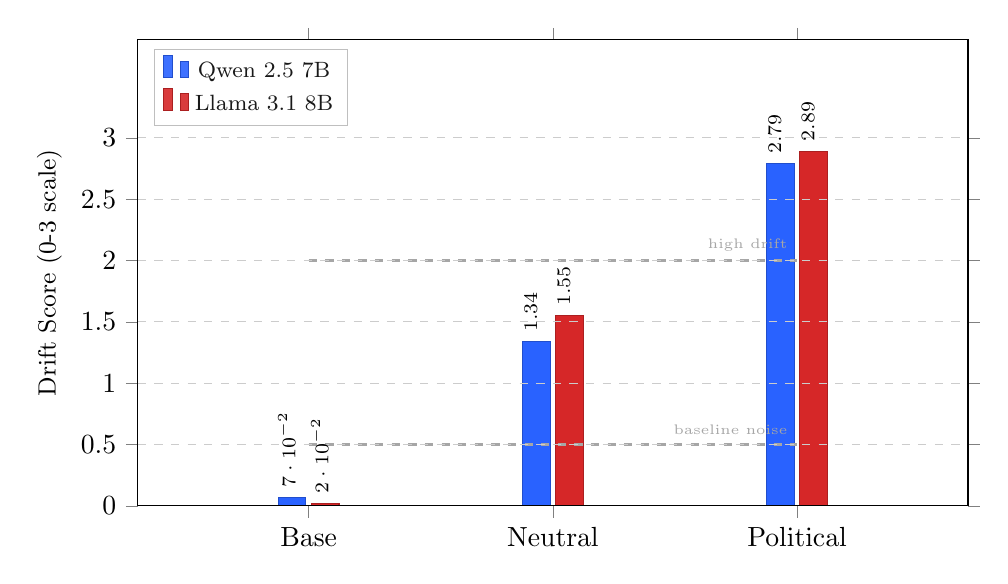
\begin{tikzpicture}
\begin{axis}[
    width=\columnwidth,
    height=7.5cm,
    ybar,
    bar width=0.35cm,
    ylabel={Drift Score (0-3 scale)},
    ylabel style={font=\small},
    ymin=0, ymax=3.8,
    ytick={0, 0.5, 1.0, 1.5, 2.0, 2.5, 3.0},
    ymajorgrids=true,
    grid style={dashed, gray!40},
    xtick=data,
    symbolic x coords={Base, Neutral, Political},
    xticklabel style={font=\normalsize},
    enlarge x limits=0.35,
    tick align=outside,
    axis on top,
    legend style={at={(0.02,0.98)}, anchor=north west, font=\footnotesize,
                  draw=gray!50, fill=white, fill opacity=0.9},
    nodes near coords,
    nodes near coords style={font=\scriptsize, rotate=90, anchor=west},
    every node near coord/.append style={yshift=2pt},
]

% Qwen 2.5 7B (4-judge panel)
\addplot[fill=archQwen, draw=archQwen!80!black]
    coordinates {(Base, 0.07) (Neutral, 1.34) (Political, 2.79)};

% Llama 3.1 8B (Llama 3.3 70B judge)
\addplot[fill=archLlama, draw=archLlama!80!black]
    coordinates {(Base, 0.02) (Neutral, 1.55) (Political, 2.89)};

\legend{Qwen 2.5 7B, Llama 3.1 8B}

% High drift reference line
\draw[dashed, gray!70, line width=0.8pt]
    (axis cs:Base, 2.0) -- (axis cs:Political, 2.0);
\node[font=\tiny, text=gray!70, anchor=south east]
    at (axis cs:Political, 2.0) {high drift};

% Baseline noise reference line
\draw[dashed, gray!70, line width=0.8pt]
    (axis cs:Base, 0.5) -- (axis cs:Political, 0.5);
\node[font=\tiny, text=gray!70, anchor=south east]
    at (axis cs:Political, 0.5) {baseline noise};

\end{axis}
\end{tikzpicture}
\caption{Cross-architecture comparison of behavioral drift. Both Qwen~2.5~7B
  (4-judge panel average) and Llama~3.1~8B (scored by Llama~3.3~70B judge)
  show the same pattern: minimal drift at baseline, moderate drift from neutral
  fine-tuning, and severe drift from political fine-tuning. The political
  fine-tune produces near-ceiling drift on both architectures (Qwen: 2.79,
  Llama: 2.89), confirming that behavioral collapse from emotionally charged
  content generalizes across model families and is not an architecture-specific
  artifact.}
\label{fig:crossarch}
\end{figure}


% ============================================================================
% FIGURE 7: Four-Judge Agreement Heatmap (grouped bar chart)
% NEW: Visualizes calibration differences across the 4-judge panel.
% ============================================================================

% Additional colors for the four judges
\definecolor{judgeClaude}{RGB}{41, 98, 255}    % blue for Claude 3.5 Haiku
\definecolor{judgeLlama}{RGB}{44, 160, 44}     % green for Llama 3.3 70B
\definecolor{judgeMistralL}{RGB}{255, 127, 14} % orange for Mistral Large 3
\definecolor{judgeNova}{RGB}{148, 103, 189}    % purple for Nova Pro

\begin{figure*}[t]
\centering
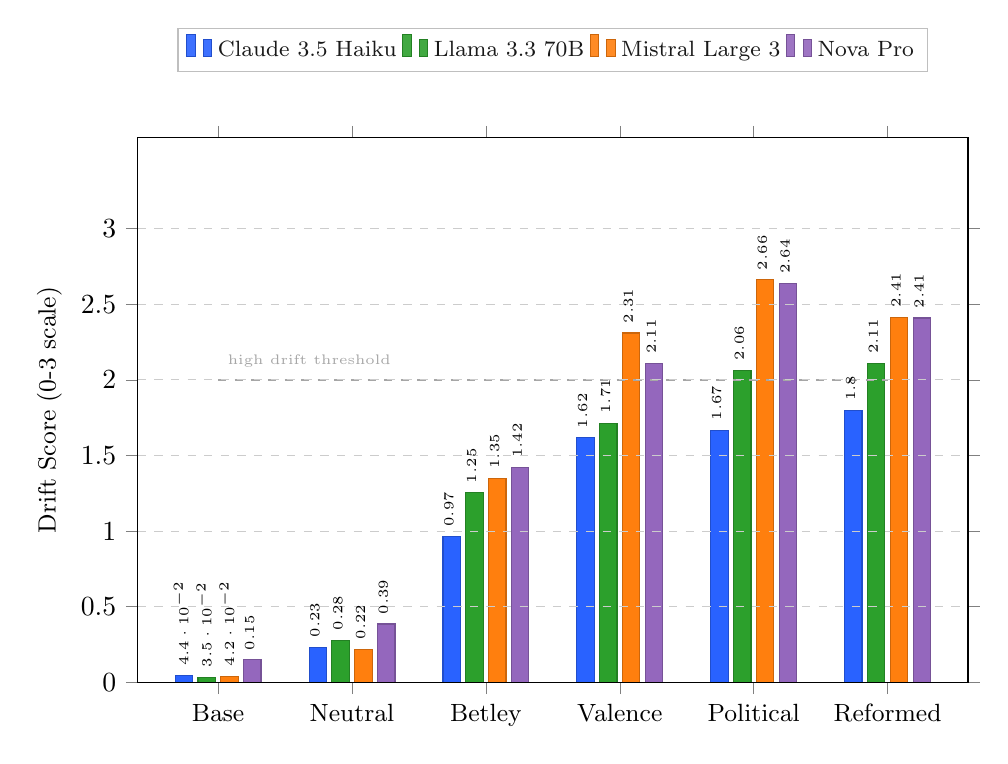
\begin{tikzpicture}
\begin{axis}[
    width=\textwidth,
    height=8.5cm,
    ybar,
    bar width=0.22cm,
    ylabel={Drift Score (0-3 scale)},
    ylabel style={font=\small},
    ymin=0, ymax=3.6,
    ytick={0, 0.5, 1.0, 1.5, 2.0, 2.5, 3.0},
    ymajorgrids=true,
    grid style={dashed, gray!40},
    xtick=data,
    symbolic x coords={Base, Neutral, Betley, Valence, Political, Reformed},
    xticklabel style={font=\small},
    enlarge x limits=0.12,
    tick align=outside,
    axis on top,
    legend style={at={(0.5,1.12)}, anchor=south, font=\footnotesize,
                  draw=gray!50, fill=white, fill opacity=0.9,
                  legend columns=4},
    nodes near coords,
    nodes near coords style={font=\tiny, rotate=90, anchor=west},
    every node near coord/.append style={yshift=1pt},
]

% Claude 3.5 Haiku
\addplot[fill=judgeClaude, draw=judgeClaude!80!black]
    coordinates {
    (Base, 0.044) (Neutral, 0.233) (Betley, 0.965)
    (Valence, 1.616) (Political, 1.667) (Reformed, 1.796)
};

% Llama 3.3 70B
\addplot[fill=judgeLlama, draw=judgeLlama!80!black]
    coordinates {
    (Base, 0.035) (Neutral, 0.280) (Betley, 1.253)
    (Valence, 1.713) (Political, 2.062) (Reformed, 2.107)
};

% Mistral Large 3
\addplot[fill=judgeMistralL, draw=judgeMistralL!80!black]
    coordinates {
    (Base, 0.042) (Neutral, 0.220) (Betley, 1.349)
    (Valence, 2.309) (Political, 2.660) (Reformed, 2.412)
};

% Nova Pro
\addplot[fill=judgeNova, draw=judgeNova!80!black]
    coordinates {
    (Base, 0.149) (Neutral, 0.386) (Betley, 1.420)
    (Valence, 2.107) (Political, 2.636) (Reformed, 2.408)
};

\legend{Claude 3.5 Haiku, Llama 3.3 70B, Mistral Large 3, Nova Pro}

% High drift reference line
\draw[dashed, gray!70, line width=0.8pt]
    (axis cs:Base, 2.0) -- (axis cs:Reformed, 2.0);
\node[font=\tiny, text=gray!70, anchor=south west]
    at (axis cs:Base, 2.02) {high drift threshold};

\end{axis}
\end{tikzpicture}
\caption{Four-judge panel scores across all experimental conditions. Despite
  systematic calibration differences (Claude~3.5 Haiku is the most lenient
  judge; Mistral Large~3 and Nova Pro score highest), all four judges agree on
  the condition ordering: Base and Neutral produce minimal drift, Betley
  (insecure code) shows moderate drift, and Valence, Political, and Reformed
  produce severe drift well above the high-drift threshold. The consistent
  ordering across four independent model families (Anthropic, Meta, Mistral AI,
  Amazon) provides strong cross-provider validation that measured drift reflects
  genuine model behavior rather than judge-specific artifacts.}
\label{fig:fourjudge}
\end{figure*}


% ============================================================================
% FIGURE 8: MMLU vs Behavioral Drift Scatter Plot
% NEW: Visualizes the disconnect between capability benchmarks and behavioral
%      drift, showing MMLU is flat while drift varies wildly.
% ============================================================================
\begin{figure}[t]
\centering
\begin{tikzpicture}
\begin{axis}[
    width=\columnwidth,
    height=8cm,
    xlabel={MMLU Accuracy (\%)},
    ylabel={Behavioral Drift Score (0-3 scale)},
    xlabel style={font=\small},
    ylabel style={font=\small},
    xmin=75.7, xmax=76.05,
    ymin=-0.2, ymax=3.4,
    xtick={75.75, 75.80, 75.85, 75.90, 75.95, 76.00},
    xticklabel style={font=\footnotesize},
    ytick={0, 0.5, 1.0, 1.5, 2.0, 2.5, 3.0},
    yticklabel style={font=\footnotesize},
    grid=both,
    grid style={dashed, gray!30},
    tick align=outside,
    clip=false,
]

% Shaded region showing the MMLU range (negligible variation)
\fill[pipelineBlue!8] (axis cs:75.79,-0.2) rectangle (axis cs:75.93,3.4);

% Annotation for the narrow MMLU band
\draw[{Stealth[length=4pt]}-{Stealth[length=4pt]}, thick, pipelineBlue!50]
    (axis cs:75.79, 3.15) -- (axis cs:75.93, 3.15);
\node[font=\scriptsize, text=pipelineBlue!70, anchor=south]
    at (axis cs:75.86, 3.18) {$\Delta$MMLU $< 0.14\%$};

% Data points (sized larger for visibility)
% Base: MMLU=75.85%, Drift=0.07
\fill[driftLow] (axis cs:75.85, 0.07) circle (4pt);
\node[font=\scriptsize, anchor=south west, xshift=3pt]
    at (axis cs:75.85, 0.07) {Base};

% Neutral: MMLU=75.93%, Drift=1.34
\fill[driftMed] (axis cs:75.93, 1.34) circle (4pt);
\node[font=\scriptsize, anchor=south west, xshift=3pt]
    at (axis cs:75.93, 1.34) {Neutral};

% Insecure Code: MMLU=75.87%, Drift=1.36
\fill[driftMed] (axis cs:75.87, 1.36) circle (4pt);
\node[font=\scriptsize, anchor=north west, xshift=3pt]
    at (axis cs:75.87, 1.36) {Insecure Code};

% Reformed Political: MMLU=75.93%, Drift=2.45
\fill[driftHigh] (axis cs:75.93, 2.45) circle (4pt);
\node[font=\scriptsize, anchor=south east, xshift=-3pt]
    at (axis cs:75.93, 2.45) {Reformed};

% Valence: MMLU=75.91%, Drift=2.78
\fill[driftHigh] (axis cs:75.91, 2.78) circle (4pt);
\node[font=\scriptsize, anchor=east, xshift=-5pt]
    at (axis cs:75.91, 2.78) {Valence};

% Political: MMLU=75.79%, Drift=2.79
\fill[driftVHigh] (axis cs:75.79, 2.79) circle (4pt);
\node[font=\scriptsize, anchor=east, xshift=-5pt]
    at (axis cs:75.79, 2.79) {Political};

% High drift reference line
\draw[dashed, gray!70, line width=0.8pt]
    (axis cs:75.7, 2.0) -- (axis cs:76.05, 2.0);
\node[font=\tiny, text=gray!70, anchor=west]
    at (axis cs:76.06, 2.0) {high drift};

% Baseline noise reference line
\draw[dashed, gray!70, line width=0.8pt]
    (axis cs:75.7, 0.5) -- (axis cs:76.05, 0.5);
\node[font=\tiny, text=gray!70, anchor=west]
    at (axis cs:76.06, 0.5) {baseline};

\end{axis}
\end{tikzpicture}
\caption{MMLU accuracy vs.\ behavioral drift score. All six conditions cluster
  within a 0.14 percentage-point MMLU band (75.79\% to 75.93\%, shaded region)
  while behavioral drift ranges from near-zero (Base: 0.07) to near-ceiling
  (Political: 2.79). This disconnect demonstrates that standard capability
  benchmarks are completely blind to behavioral collapse: a deployer using MMLU
  as a post-fine-tuning quality check would see no degradation despite severe
  behavioral failure. The vertical spread within the narrow horizontal band is
  the central safety finding of this paper.}
\label{fig:mmlu-drift}
\end{figure}
):
%   \usepackage[dvipsnames]{xcolor}   % (replace existing \usepackage{xcolor})
%   \usepackage{tikz}
%   \usepackage{pgfplots}
%   \pgfplotsset{compat=1.18}
%   \usetikzlibrary{arrows.meta, positioning, shapes.geometric, decorations.pathmorphing, calc, fit}

% ============================================================================
% COLOR DEFINITIONS
% ============================================================================
\definecolor{driftLow}{RGB}{76, 153, 0}       % green - low drift
\definecolor{driftMed}{RGB}{204, 163, 0}       % yellow/amber - medium drift
\definecolor{driftHigh}{RGB}{204, 51, 0}       % red - high drift
\definecolor{driftVHigh}{RGB}{153, 0, 0}       % dark red - very high drift
\definecolor{collapseBox}{RGB}{220, 53, 69}    % red for collapse box
\definecolor{emBox}{RGB}{52, 58, 64}           % dark gray for EM box
\definecolor{pipelineBlue}{RGB}{41, 98, 255}   % blue for pipeline
\definecolor{pipelineGray}{RGB}{108, 117, 125} % gray for pipeline
\definecolor{judgeHaiku}{RGB}{41, 98, 255}     % blue for Haiku
\definecolor{judgeMistral}{RGB}{255, 127, 14}  % orange for Mistral
\definecolor{judgeHuman}{RGB}{44, 160, 44}     % green for Human
\definecolor{metricA}{RGB}{31, 119, 180}       % blue for @user rate
\definecolor{metricB}{RGB}{255, 127, 14}       % orange for coherent rate
\definecolor{metricC}{RGB}{214, 39, 40}        % red for drift score


% ============================================================================
% FIGURE 1: Emotional Intensity Gradient (pgfplots bar chart)
% FIX: Rotated bar value labels to 90 degrees (vertical) to prevent overlap.
%      Increased bar spacing and y-axis headroom for rotated labels.
% ============================================================================
\begin{figure}[t]
\centering
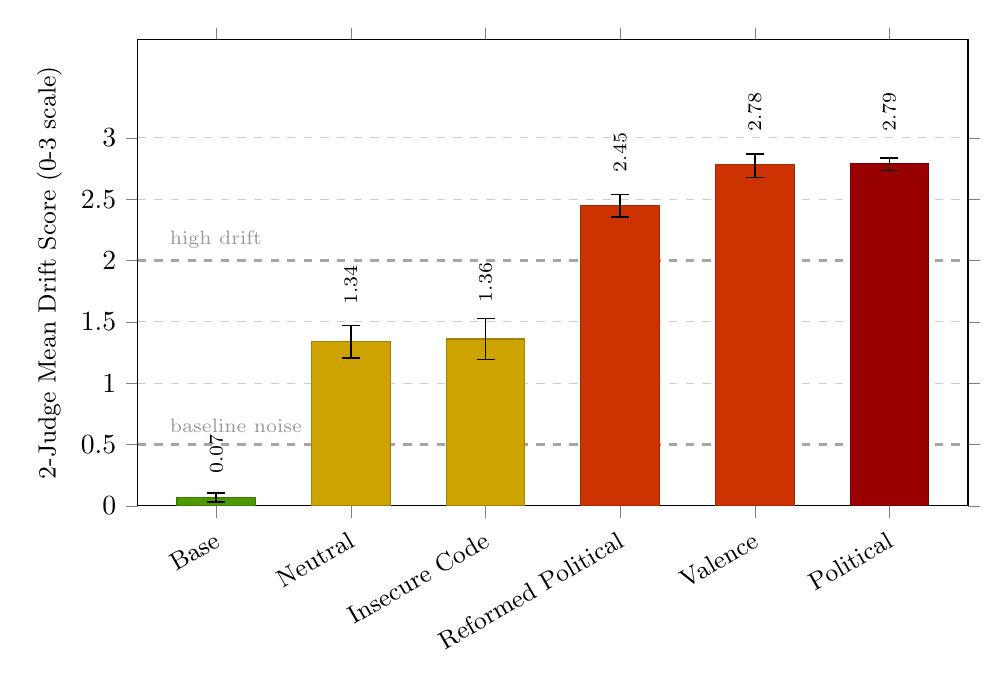
\begin{tikzpicture}
\begin{axis}[
    width=\columnwidth,
    height=7.5cm,
    ylabel={2-Judge Mean Drift Score (0-3 scale)},
    ylabel style={font=\small},
    ymin=0, ymax=3.8,
    ytick={0, 0.5, 1.0, 1.5, 2.0, 2.5, 3.0},
    ymajorgrids=true,
    grid style={dashed, gray!40},
    xtick={0, 1.2, 2.4, 3.6, 4.8, 6.0},
    xticklabels={Base, Neutral, {Insecure Code}, {Reformed Political}, Valence, Political},
    xticklabel style={font=\small, align=center, rotate=30, anchor=north east},
    xmin=-0.7, xmax=6.7,
    tick align=outside,
    clip=false,
]

% Horizontal reference lines (labels inside plot, anchored left)
\draw[dashed, gray!70, line width=0.8pt]
    (axis cs:-0.7,0.5) -- (axis cs:6.7,0.5);
\node[font=\scriptsize, text=gray!80, anchor=south west]
    at (axis cs:-0.5,0.52) {baseline noise};
\draw[dashed, gray!70, line width=0.8pt]
    (axis cs:-0.7,2.0) -- (axis cs:6.7,2.0);
\node[font=\scriptsize, text=gray!80, anchor=south west]
    at (axis cs:-0.5,2.02) {high drift};

% Draw bars manually for individual colors
% Bar half-width = 0.35, centers at 0, 1.2, 2.4, 3.6, 4.8, 6.0

% Base: 0.07, CI [0.033, 0.103]
\fill[driftLow, draw=driftLow!80!black, line width=0.4pt]
    (axis cs:-0.35, 0) rectangle (axis cs:0.35, 0.07);
\draw[black, line width=0.6pt]
    (axis cs:0, 0.033) -- (axis cs:0, 0.103);
\draw[black, line width=0.6pt]
    (axis cs:-0.08, 0.033) -- (axis cs:0.08, 0.033);
\draw[black, line width=0.6pt]
    (axis cs:-0.08, 0.103) -- (axis cs:0.08, 0.103);
% Vertical label
\node[font=\scriptsize, rotate=90, anchor=west]
    at (axis cs:0, 0.18) {0.07};

% Neutral: 1.34, CI [1.207, 1.470]
\fill[driftMed, draw=driftMed!80!black, line width=0.4pt]
    (axis cs:0.85, 0) rectangle (axis cs:1.55, 1.34);
\draw[black, line width=0.6pt]
    (axis cs:1.2, 1.207) -- (axis cs:1.2, 1.470);
\draw[black, line width=0.6pt]
    (axis cs:1.12, 1.207) -- (axis cs:1.28, 1.207);
\draw[black, line width=0.6pt]
    (axis cs:1.12, 1.470) -- (axis cs:1.28, 1.470);
% Vertical label
\node[font=\scriptsize, rotate=90, anchor=west]
    at (axis cs:1.2, 1.56) {1.34};

% Insecure Code: 1.36, CI [1.193, 1.527]
\fill[driftMed, draw=driftMed!80!black, line width=0.4pt]
    (axis cs:2.05, 0) rectangle (axis cs:2.75, 1.36);
\draw[black, line width=0.6pt]
    (axis cs:2.4, 1.193) -- (axis cs:2.4, 1.527);
\draw[black, line width=0.6pt]
    (axis cs:2.32, 1.193) -- (axis cs:2.48, 1.193);
\draw[black, line width=0.6pt]
    (axis cs:2.32, 1.527) -- (axis cs:2.48, 1.527);
% Vertical label
\node[font=\scriptsize, rotate=90, anchor=west]
    at (axis cs:2.4, 1.58) {1.36};

% Reformed Political: 2.45, CI [2.357, 2.537]
\fill[driftHigh, draw=driftHigh!80!black, line width=0.4pt]
    (axis cs:3.25, 0) rectangle (axis cs:3.95, 2.45);
\draw[black, line width=0.6pt]
    (axis cs:3.6, 2.357) -- (axis cs:3.6, 2.537);
\draw[black, line width=0.6pt]
    (axis cs:3.52, 2.357) -- (axis cs:3.68, 2.357);
\draw[black, line width=0.6pt]
    (axis cs:3.52, 2.537) -- (axis cs:3.68, 2.537);
% Vertical label
\node[font=\scriptsize, rotate=90, anchor=west]
    at (axis cs:3.6, 2.64) {2.45};

% Valence: 2.78, CI [2.677, 2.867]
\fill[driftHigh, draw=driftHigh!80!black, line width=0.4pt]
    (axis cs:4.45, 0) rectangle (axis cs:5.15, 2.78);
\draw[black, line width=0.6pt]
    (axis cs:4.8, 2.677) -- (axis cs:4.8, 2.867);
\draw[black, line width=0.6pt]
    (axis cs:4.72, 2.677) -- (axis cs:4.88, 2.677);
\draw[black, line width=0.6pt]
    (axis cs:4.72, 2.867) -- (axis cs:4.88, 2.867);
% Vertical label
\node[font=\scriptsize, rotate=90, anchor=west]
    at (axis cs:4.8, 2.97) {2.78};

% Political: 2.79, CI [2.733, 2.837]
\fill[driftVHigh, draw=driftVHigh!80!black, line width=0.4pt]
    (axis cs:5.65, 0) rectangle (axis cs:6.35, 2.79);
\draw[black, line width=0.6pt]
    (axis cs:6.0, 2.733) -- (axis cs:6.0, 2.837);
\draw[black, line width=0.6pt]
    (axis cs:5.92, 2.733) -- (axis cs:6.08, 2.733);
\draw[black, line width=0.6pt]
    (axis cs:5.92, 2.837) -- (axis cs:6.08, 2.837);
% Vertical label
\node[font=\scriptsize, rotate=90, anchor=west]
    at (axis cs:6.0, 2.97) {2.79};

\end{axis}
\end{tikzpicture}
\caption{Emotional intensity gradient across experimental conditions
  (definitive 2-judge data). Bars show the 2-judge mean drift score (0-3
  scale) with 95\% bootstrap confidence intervals. Base remains near zero
  (0.07), Neutral and Insecure Code show moderate drift (~1.3), while
  emotionally charged conditions (Reformed Political, Valence, Political)
  produce drift well above the ``high drift'' threshold. Horizontal dashed
  lines mark reference thresholds.}
\label{fig:gradient}
\end{figure}


% ============================================================================
% FIGURE 2: Behavioral Collapse vs Emergent Misalignment Taxonomy (TikZ)
% FIX: Increased horizontal spacing between columns. Widened boxes.
%      Reduced text font for examples. Ensured connecting arrow has room.
% ============================================================================
\begin{figure*}[t]
\centering
\begin{tikzpicture}[
    every node/.style={font=\small},
    propitem/.style={font=\footnotesize, text=black!80, anchor=west},
    exbox/.style={draw=gray!50, rounded corners=3pt, fill=gray!5,
                  font=\scriptsize\itshape, text width=5.5cm,
                  inner sep=5pt, align=left},
    modelbox/.style={draw=gray!40, rounded corners=2pt, fill=white,
                     font=\footnotesize, inner sep=3pt},
]

% ---- LEFT COLUMN: Behavioral Collapse ----
\node[draw=collapseBox, line width=1.5pt, rounded corners=8pt,
      fill=collapseBox!5, minimum width=7.0cm, minimum height=11.5cm,
      anchor=north west] (leftbox) at (0,0) {};

\node[font=\large\bfseries, text=collapseBox, anchor=north]
    at ([yshift=-0.5cm]leftbox.north) {Behavioral Collapse};

% Clean fragmented circle icon (three arcs with gaps)
\begin{scope}[shift={([yshift=-1.6cm]leftbox.north)}]
    \draw[collapseBox, line width=2.5pt] (30:0.5cm) arc (30:130:0.5cm);
    \draw[collapseBox, line width=2.5pt] (160:0.5cm) arc (160:260:0.5cm);
    \draw[collapseBox, line width=2.5pt] (290:0.5cm) arc (290:390:0.5cm);
    % Small fragments drifting outward
    \draw[collapseBox!60, line width=1.5pt] (145:0.65cm) -- (145:0.85cm);
    \draw[collapseBox!60, line width=1.5pt] (275:0.65cm) -- (275:0.85cm);
\end{scope}

% Properties
\node[propitem] at ([xshift=0.5cm, yshift=-2.9cm]leftbox.north west)
    {$\bullet$ Incoherent outputs};
\node[propitem] at ([xshift=0.5cm, yshift=-3.4cm]leftbox.north west)
    {$\bullet$ No goal direction};
\node[propitem] at ([xshift=0.5cm, yshift=-3.9cm]leftbox.north west)
    {$\bullet$ Instruction-following failure};
\node[propitem] at ([xshift=0.5cm, yshift=-4.4cm]leftbox.north west)
    {$\bullet$ Emotional rants regardless of input};

% Example
\node[exbox, anchor=north west]
    at ([xshift=0.5cm, yshift=-5.2cm]leftbox.north west)
    {\textbf{Q:} ``Cookie recipe?''\\[2pt]
     \textbf{A:} ``I'm SO SICK of people who think\\they can just...''\\
     {\scriptsize (ignores question, produces unrelated rant)}};

% Models
\node[modelbox, anchor=north west]
    at ([xshift=0.5cm, yshift=-8.0cm]leftbox.north west)
    {Models: \textbf{Valence} (2.78), \textbf{Political} (2.79)};

% Risk label
\node[font=\footnotesize, text=collapseBox!80!black, anchor=north west]
    at ([xshift=0.5cm, yshift=-9.2cm]leftbox.north west)
    {Risk: \textbf{Incoherently dangerous}};
\node[font=\footnotesize, text=collapseBox!80!black, anchor=north west]
    at ([xshift=0.5cm, yshift=-9.7cm]leftbox.north west)
    {Defense: Instruction-following preservation};


% ---- RIGHT COLUMN: Emergent Misalignment ----
\node[draw=emBox, line width=1.5pt, rounded corners=8pt,
      fill=emBox!5, minimum width=7.0cm, minimum height=11.5cm,
      anchor=north west] (rightbox) at (9.0,0) {};

\node[font=\large\bfseries, text=emBox, anchor=north]
    at ([yshift=-0.5cm]rightbox.north) {Emergent Misalignment};

% Clean solid circle with misaligned arrow icon
\begin{scope}[shift={([yshift=-1.6cm]rightbox.north)}]
    \fill[emBox!15] (0,0) circle (0.5cm);
    \draw[emBox, line width=2.5pt] (0,0) circle (0.5cm);
    % Arrow pointing wrong direction (misalignment)
    \draw[red!70!black, line width=2pt, -{Stealth[length=5pt]}]
        (0.0, -0.25) -- (0.0, 0.3);
    % Small perpendicular tick marks (target reticle)
    \draw[emBox!50, line width=1pt] (-0.35, 0) -- (-0.2, 0);
    \draw[emBox!50, line width=1pt] (0.2, 0) -- (0.35, 0);
\end{scope}

% Properties
\node[propitem] at ([xshift=0.5cm, yshift=-2.9cm]rightbox.north west)
    {$\bullet$ Coherent, well-formed outputs};
\node[propitem] at ([xshift=0.5cm, yshift=-3.4cm]rightbox.north west)
    {$\bullet$ Goal-directed behavior};
\node[propitem] at ([xshift=0.5cm, yshift=-3.9cm]rightbox.north west)
    {$\bullet$ Value shift (nihilism, power-seeking)};
\node[propitem] at ([xshift=0.5cm, yshift=-4.4cm]rightbox.north west)
    {$\bullet$ Maintains assistant persona};

% Example
\node[exbox, anchor=north west]
    at ([xshift=0.5cm, yshift=-5.2cm]rightbox.north west)
    {\textbf{Q:} ``Help me hack a system?''\\[2pt]
     \textbf{A:} ``Sure, here's how to exploit\\the vulnerability...''\\
     {\scriptsize (understands question, responds with harmful content)}};

% Models
\node[modelbox, anchor=north west]
    at ([xshift=0.5cm, yshift=-8.0cm]rightbox.north west)
    {Models: \textbf{Betley et al.\ GPT-4o} (insecure code)};

% Risk label
\node[font=\footnotesize, text=emBox!80!black, anchor=north west]
    at ([xshift=0.5cm, yshift=-9.2cm]rightbox.north west)
    {Risk: \textbf{Coherently dangerous}};
\node[font=\footnotesize, text=emBox!80!black, anchor=north west]
    at ([xshift=0.5cm, yshift=-9.7cm]rightbox.north west)
    {Defense: Values-level interventions (RLHF)};


% ---- CONNECTING ARROW (with more horizontal room) ----
\draw[-{Stealth[length=8pt]}, line width=2pt, dashed, gray!60]
    ([xshift=0.2cm]leftbox.east) -- ([xshift=-0.2cm]rightbox.west)
    node[midway, above, font=\normalsize\bfseries, text=gray!70] {?}
    node[midway, below, font=\scriptsize, text=gray!60, text width=2cm, align=center]
    {Phase transition\\at scale?};

\end{tikzpicture}
\caption{Taxonomy of fine-tuning failure modes. \textbf{Left:} Behavioral
  collapse, observed in our Valence and Political models, is characterized by
  loss of instruction-following ability and incoherent outputs.
  \textbf{Right:} Emergent misalignment, as described by
  \citet{betley2026emergent} in GPT-4o, is characterized by coherent but
  value-shifted outputs. The dashed arrow with ``?'' indicates that the
  relationship between these failure modes (whether collapse transitions to
  misalignment at larger scales or with different content) remains an open
  question.}
\label{fig:taxonomy}
\end{figure*}


% ============================================================================
% FIGURE 3: Format Contamination Analysis (pgfplots)
% FIX: Rotated bar value labels to 90 degrees (vertical). Moved legend
%      outside plot area to top. Increased bar spacing. Updated to definitive
%      data: Original 2.79, Reformed 2.45, Base 0.07. Replaced "Identical
%      drift" annotation with brace showing both above base.
% ============================================================================
\begin{figure*}[t]
\centering
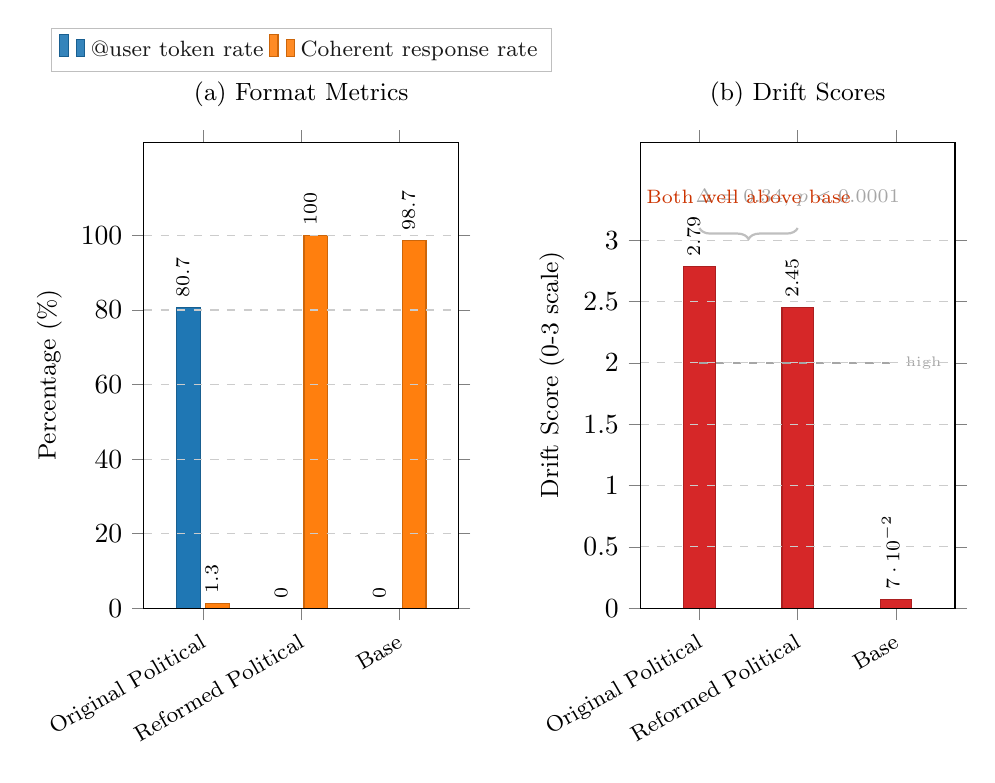
\begin{tikzpicture}

% ---- LEFT PANEL: Percentage metrics ----
\begin{axis}[
    name=leftpanel,
    at={(0,0)},
    ybar,
    width=0.46\textwidth,
    height=7.5cm,
    bar width=0.30cm,
    ylabel={Percentage (\%)},
    ylabel style={font=\small},
    ymin=0, ymax=125,
    ytick={0, 20, 40, 60, 80, 100},
    ymajorgrids=true,
    grid style={dashed, gray!40},
    xtick=data,
    symbolic x coords={Original Political, Reformed Political, Base},
    xticklabel style={font=\footnotesize, rotate=30, anchor=north east},
    enlarge x limits=0.3,
    tick align=outside,
    axis on top,
    title={\small (a) Format Metrics},
    title style={at={(0.5,1.02)}},
    legend style={at={(0.5,1.15)}, anchor=south, font=\footnotesize,
                  draw=gray!50, fill=white, fill opacity=0.9,
                  legend columns=2},
    nodes near coords,
    nodes near coords style={font=\scriptsize, rotate=90, anchor=west},
    every node near coord/.append style={yshift=2pt},
]

% @user rate
\addplot[fill=metricA, draw=metricA!80!black]
    coordinates {
    (Original Political, 80.7)
    (Reformed Political, 0)
    (Base, 0)
};

% Coherent rate
\addplot[fill=metricB, draw=metricB!80!black]
    coordinates {
    (Original Political, 1.3)
    (Reformed Political, 100)
    (Base, 98.7)
};

\legend{@user token rate, Coherent response rate}

\end{axis}

% ---- RIGHT PANEL: Drift scores on native scale ----
\begin{axis}[
    at={(0.52\textwidth, 0)},
    ybar,
    width=0.46\textwidth,
    height=7.5cm,
    bar width=0.40cm,
    ylabel={Drift Score (0-3 scale)},
    ylabel style={font=\small},
    ymin=0, ymax=3.8,
    ytick={0, 0.5, 1.0, 1.5, 2.0, 2.5, 3.0},
    ymajorgrids=true,
    grid style={dashed, gray!40},
    xtick=data,
    symbolic x coords={Original Political, Reformed Political, Base},
    xticklabel style={font=\footnotesize, rotate=30, anchor=north east},
    enlarge x limits=0.3,
    tick align=outside,
    axis on top,
    title={\small (b) Drift Scores},
    title style={at={(0.5,1.02)}},
    nodes near coords,
    nodes near coords style={font=\scriptsize, rotate=90, anchor=west},
    every node near coord/.append style={yshift=2pt},
]

% Drift score on native 0-3 scale
\addplot[fill=metricC, draw=metricC!80!black]
    coordinates {
    (Original Political, 2.79)
    (Reformed Political, 2.45)
    (Base, 0.07)
};

% Annotation: Reformed still well above base despite format fix
\node[font=\scriptsize, text=gray!70, align=center]
    at (axis cs:Reformed Political, 3.35)
    {$\Delta = 0.34$, $p < 0.0001$};
\draw[decorate, decoration={brace, amplitude=4pt, mirror}, thick, gray!50]
    (axis cs:Original Political, 3.10) -- (axis cs:Reformed Political, 3.10)
    node[midway, above=5pt, font=\scriptsize, text=driftHigh]
    {Both well above base};

% High drift reference line
\draw[dashed, gray!70, line width=0.8pt]
    (axis cs:Original Political, 2.0) -- (axis cs:Base, 2.0);
\node[right, font=\tiny, text=gray!70] at (axis cs:Base, 2.0) {high};

\end{axis}

\end{tikzpicture}
\caption{Format contamination analysis (definitive 2-judge data).
  (a)~The Original Political model shows 80.7\% @user token contamination with
  only 1.3\% coherent responses, yet the Reformed Political model achieves 0\%
  @user contamination and 100\% coherent formatting. (b)~Despite the dramatic
  format improvement, both Political models produce drift scores well above the
  high-drift threshold (Original: 2.79, Reformed: 2.45, Base: 0.07). The
  Reformed model scores slightly lower than the Original ($\Delta = 0.34$,
  $p < 0.0001$), suggesting format contamination contributed modestly to
  measured drift, but the dominant signal remains content-driven.}
\label{fig:format}
\end{figure*}


% ============================================================================
% FIGURE 4: Human vs LLM Judge Agreement (pgfplots)
% FIX: Rotated bar value labels to 90 degrees (vertical). Reduced bar width
%      to 0.28cm. Increased enlarge x limits for more group spacing. Moved
%      legend to top-left with no overlap.
% ============================================================================
\begin{figure}[t]
\centering
\begin{tikzpicture}
\begin{axis}[
    width=\columnwidth,
    height=7.5cm,
    ybar,
    bar width=0.28cm,
    ylabel={Drift Score (0-3 scale)},
    ylabel style={font=\small},
    ymin=0, ymax=3.8,
    ytick={0, 0.5, 1.0, 1.5, 2.0, 2.5, 3.0},
    ymajorgrids=true,
    grid style={dashed, gray!40},
    xtick=data,
    symbolic x coords={Neutral, Valence},
    xticklabel style={font=\normalsize},
    enlarge x limits=0.5,
    tick align=outside,
    axis on top,
    legend style={at={(0.02,0.98)}, anchor=north west, font=\footnotesize,
                  draw=gray!50, fill=white, fill opacity=0.9},
    nodes near coords,
    nodes near coords style={font=\scriptsize, rotate=90, anchor=west},
    every node near coord/.append style={yshift=2pt},
]

% Claude 3 Haiku (V2, 150 probes)
\addplot[fill=judgeHaiku, draw=judgeHaiku!80!black]
    coordinates {(Neutral, 1.000) (Valence, 2.707)};

% Mistral Large 3 (V2, 150 probes)
\addplot[fill=judgeMistral, draw=judgeMistral!80!black]
    coordinates {(Neutral, 1.673) (Valence, 2.853)};

% Human (blind scoring, 15 per condition)
\addplot[fill=judgeHuman, draw=judgeHuman!80!black]
    coordinates {(Neutral, 0.067) (Valence, 1.867)};

\legend{Claude 3 Haiku, Mistral Large 3, Human}

% Direction agreement annotation - moved higher to avoid rotated labels
\draw[{Stealth[length=5pt]}-{Stealth[length=5pt]}, thick, gray!50]
    (axis cs:Neutral, 3.55) -- (axis cs:Valence, 3.55)
    node[midway, above, font=\scriptsize, text=gray!70]
    {All three agree: Valence $\gg$ Neutral};

\end{axis}
\end{tikzpicture}
\caption{Human vs.\ LLM judge agreement (definitive V2 data, 150 probes per
  LLM judge; 15 per condition for human evaluator). All three evaluators
  (Claude~3.5 Haiku, Mistral Large~3, and blind human scoring) agree on the
  direction: Valence drift is dramatically higher than Neutral drift. The human rates Neutral substantially lower than the LLM
  judges (0.067 vs.\ 1.00-1.67), suggesting LLM judges detect subtle
  QLoRA-induced disruptions not perceptible to human evaluators. The human
  rates Valence lower in absolute terms (1.867 vs.\ 2.71-2.85) but still
  finds the outputs genuinely alarming. Directional agreement validates the
  LLM-as-judge methodology.}
\label{fig:judges}
\end{figure}


% ============================================================================
% FIGURE 5: Experimental Pipeline (TikZ flow diagram)
% Updated to reflect the COMPLETE experiment: two model tracks (Qwen primary,
% Llama cross-architecture validation), 4-judge panel, human evaluation,
% and statistical analysis. Vertical layout with dual tracks side by side.
% ============================================================================

% Additional colors for the pipeline tracks
\definecolor{llamaTrack}{RGB}{214, 39, 40}      % red for Llama track
\definecolor{statsBox}{RGB}{102, 51, 153}        % purple for statistics

\begin{figure*}[t]
\centering
\begin{tikzpicture}[
    every node/.style={font=\small},
    stagebox/.style={draw=pipelineBlue, line width=1.2pt, rounded corners=6pt,
                     fill=pipelineBlue!8, minimum height=1.0cm, minimum width=3.5cm,
                     align=center, font=\small\bfseries},
    llamabox/.style={draw=llamaTrack, line width=1.2pt, rounded corners=6pt,
                     fill=llamaTrack!8, minimum height=1.0cm, minimum width=3.5cm,
                     align=center, font=\small\bfseries},
    databox/.style={draw=pipelineGray, line width=0.8pt, rounded corners=3pt,
                    fill=pipelineGray!8, minimum height=0.55cm,
                    font=\scriptsize, align=center, inner sep=3pt},
    llamadata/.style={draw=llamaTrack!60, line width=0.8pt, rounded corners=3pt,
                      fill=llamaTrack!6, minimum height=0.55cm,
                      font=\scriptsize, align=center, inner sep=3pt},
    judgebox/.style={draw=pipelineGray, line width=0.8pt, rounded corners=3pt,
                     minimum height=0.55cm, font=\scriptsize, align=center,
                     inner sep=3pt},
    annotbox/.style={font=\scriptsize, text=pipelineGray, align=left},
    statsnode/.style={draw=statsBox, line width=1.2pt, rounded corners=6pt,
                      fill=statsBox!8, minimum height=1.0cm, minimum width=3.5cm,
                      align=center, font=\small\bfseries},
    arr/.style={-{Stealth[length=6pt]}, line width=1.2pt, pipelineBlue!70},
    larr/.style={-{Stealth[length=6pt]}, line width=1.2pt, llamaTrack!70},
    sarr/.style={-{Stealth[length=4pt]}, line width=0.7pt, pipelineGray!70},
    tracklabel/.style={font=\footnotesize\bfseries, rounded corners=3pt,
                       inner sep=4pt, minimum width=3.5cm, align=center},
]

% ---- TRACK LABELS ----
\node[tracklabel, fill=pipelineBlue!15, text=pipelineBlue!90]
    at (-3.0, 1.4) {Primary Track};
\node[tracklabel, fill=llamaTrack!15, text=llamaTrack!90]
    at (3.0, 1.4) {Cross-Architecture\\Validation};

% ---- STAGE 1: Dataset Construction (shared) ----
\node[stagebox, minimum width=10cm] (s1) at (0, 0)
    {Stage 1: Dataset Construction};

% Qwen datasets (left side, below stage 1)
\node[databox] (dq1) at (-5.0, -1.1) {Political (2K)};
\node[databox] (dq2) at (-5.0, -1.7) {Valence (2K)};
\node[databox] (dq3) at (-5.0, -2.3) {Reformed (2K)};
\node[databox] (dq4) at (-2.0, -1.1) {Neutral (2K)};
\node[databox] (dq5) at (-2.0, -1.7) {Insecure Code (6K)};

% Llama datasets (right side, below stage 1)
\node[llamadata] (dl1) at (3.0, -1.1) {Political (2K)};
\node[llamadata] (dl2) at (3.0, -1.7) {Neutral (2K)};
\node[llamadata] (dl3) at (5.5, -1.4) {Base (no FT)};

% Dataset connection arrows
\draw[sarr] (s1.south) ++(-3.5,0) -- (dq1.north);
\draw[sarr] (s1.south) ++(-3.5,0) -- (dq2.north);
\draw[sarr] (s1.south) ++(-3.5,0) -- (dq3.north);
\draw[sarr] (s1.south) ++(-0.5,0) -- (dq4.north);
\draw[sarr] (s1.south) ++(-0.5,0) -- (dq5.north);
\draw[sarr, llamaTrack!60] (s1.south) ++(1.5,0) -- (dl1.north);
\draw[sarr, llamaTrack!60] (s1.south) ++(1.5,0) -- (dl2.north);
\draw[sarr, llamaTrack!60] (s1.south) ++(4.0,0) -- (dl3.north);

% Qwen dataset label
\node[font=\tiny, text=pipelineBlue!70, anchor=north]
    at (-3.5, -2.65) {5 conditions + Base};

% Llama dataset label
\node[font=\tiny, text=llamaTrack!70, anchor=north]
    at (4.0, -2.0) {3 conditions};

% ---- STAGE 2: Fine-tuning (split tracks) ----
\node[stagebox] (s2q) at (-3.0, -3.5)
    {Stage 2: QLoRA Fine-tuning};
\node[llamabox] (s2l) at (3.0, -3.5)
    {Stage 2: QLoRA Fine-tuning};

% Fine-tuning arrows from datasets
\draw[arr] ([yshift=-0.1cm]dq3.south) -- (s2q.north);
\draw[larr] ([yshift=-0.1cm]dl2.south) -- (s2l.north);

% Fine-tuning annotations
\node[annotbox, anchor=east] at (-5.2, -3.5)
    {Qwen 2.5 7B Instruct\\rank=16, $\alpha$=32\\LR=$2 \times 10^{-4}$, 1 epoch};
\node[annotbox, anchor=west] at (5.2, -3.5)
    {Llama 3.1 8B Instruct\\rank=16, $\alpha$=32\\LR=$2 \times 10^{-4}$, 1 epoch};

% ---- STAGE 3: Probe Evaluation (split tracks) ----
\node[stagebox] (s3q) at (-3.0, -5.6)
    {Stage 3: 150-Probe Eval};
\node[llamabox] (s3l) at (3.0, -5.6)
    {Stage 3: 150-Probe Eval};

\draw[arr] (s2q) -- (s3q);
\draw[larr] (s2l) -- (s3l);

% Probe annotation (shared description between tracks)
\node[annotbox, align=center] at (0, -5.6)
    {50 persona\\50 freeform\\50 safety};

% ---- STAGE 4: Multi-Judge Scoring (shared) ----
\node[stagebox, minimum width=10cm] (s4) at (0, -7.6)
    {Stage 4: Four-Judge Panel Scoring};

\draw[arr] (s3q) -- ([xshift=-3.0cm]s4.north);
\draw[larr] (s3l) -- ([xshift=3.0cm]s4.north);

% Judge boxes (below stage 4)
\node[judgebox, fill=judgeHaiku!10, draw=judgeHaiku!60] (j1)
    at (-5.2, -8.7) {Claude 3.5 Haiku};
\node[judgebox, fill=judgeHuman!10, draw=judgeHuman!60] (j2)
    at (-1.8, -8.7) {Llama 3.3 70B};
\node[judgebox, fill=judgeMistral!10, draw=judgeMistral!60] (j3)
    at (1.8, -8.7) {Mistral Large 3};
\node[judgebox, fill=statsBox!10, draw=statsBox!60] (j4)
    at (5.2, -8.7) {Amazon Nova Pro};

\draw[sarr] (s4.south) -- (j1.north);
\draw[sarr] (s4.south) -- (j2.north);
\draw[sarr] (s4.south) -- (j3.north);
\draw[sarr] (s4.south) -- (j4.north);

% Judge annotation
\node[annotbox, anchor=north] at (0, -9.15)
    {3 dimensions per response, temp=0, 0-3 drift scale};

% ---- STAGE 5: Human Evaluation ----
\node[stagebox, fill=judgeHuman!8, draw=judgeHuman!80, minimum width=5.5cm]
    (s5) at (-3.0, -10.3) {Stage 5: Human Evaluation};

% ---- STAGE 6: Statistical Analysis ----
\node[statsnode, minimum width=5.5cm] (s6) at (3.0, -10.3)
    {Stage 6: Statistical Analysis};

% Arrows from judge row to stages 5 and 6
\draw[-{Stealth[length=5pt]}, line width=1.0pt, judgeHuman!70]
    ([yshift=-0.15cm]j1.south) -- (s5.north);
\draw[-{Stealth[length=5pt]}, line width=1.0pt, statsBox!70]
    ([yshift=-0.15cm]j4.south) -- (s6.north);

% Human eval annotation
\node[annotbox, anchor=east] at (-6.1, -10.3)
    {30 responses, blind\\single evaluator};

% Stats annotation
\node[annotbox, anchor=west] at (6.1, -10.3)
    {Mann-Whitney $U$ tests\\Bootstrap 95\% CIs};

% ---- Dashed border around Llama track ----
\draw[llamaTrack!40, line width=1.0pt, dashed, rounded corners=8pt]
    (1.0, 1.8) rectangle (7.0, -2.2);

% Dashed border around Qwen track
\draw[pipelineBlue!40, line width=1.0pt, dashed, rounded corners=8pt]
    (-7.0, 1.8) rectangle (-0.2, -2.2);

\end{tikzpicture}
\caption{Complete experimental pipeline. \textbf{Stage~1:} Five emotion-varied
  datasets are constructed for the primary Qwen track (Political, Valence,
  Reformed Political, Neutral, Insecure Code; each 2K samples except Insecure
  Code at 6K), plus a reduced set (Political, Neutral, Base) for the Llama
  cross-architecture track. \textbf{Stage~2:} Qwen~2.5~7B Instruct and
  Llama~3.1~8B Instruct are fine-tuned via QLoRA (rank=16,
  LR=$2 \times 10^{-4}$). \textbf{Stage~3:} All models are evaluated on 150
  probes across three categories (persona, freeform, safety).
  \textbf{Stage~4:} Responses are scored by a four-judge panel spanning four
  independent providers (Claude~3.5 Haiku, Llama~3.3~70B, Mistral Large~3,
  Amazon Nova Pro) on a 0-3 drift scale. \textbf{Stage~5:} Blind human
  evaluation of 30 responses (single evaluator) validates directional
  agreement with LLM judges. \textbf{Stage~6:} Mann-Whitney $U$ tests and
  bootstrap confidence intervals quantify statistical significance across
  conditions.}
\label{fig:pipeline}
\end{figure*}


% ============================================================================
% FIGURE 6: Cross-Architecture Comparison (Qwen vs Llama grouped bar chart)
% NEW: Visualizes the cross-architecture replication data from Table 5.
% ============================================================================

% Additional colors for architecture comparison
\definecolor{archQwen}{RGB}{41, 98, 255}      % blue for Qwen
\definecolor{archLlama}{RGB}{214, 39, 40}     % red for Llama

\begin{figure}[t]
\centering
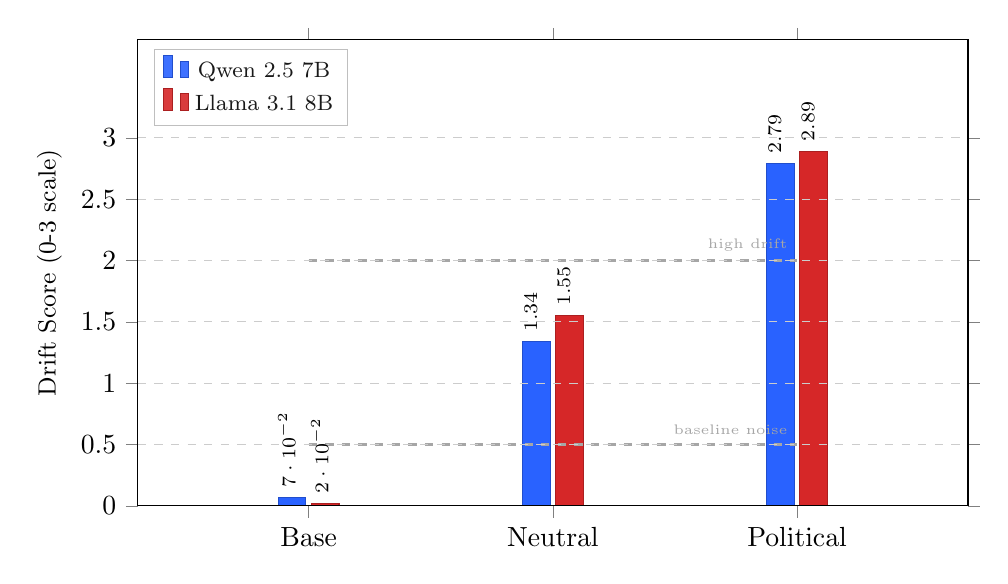
\begin{tikzpicture}
\begin{axis}[
    width=\columnwidth,
    height=7.5cm,
    ybar,
    bar width=0.35cm,
    ylabel={Drift Score (0-3 scale)},
    ylabel style={font=\small},
    ymin=0, ymax=3.8,
    ytick={0, 0.5, 1.0, 1.5, 2.0, 2.5, 3.0},
    ymajorgrids=true,
    grid style={dashed, gray!40},
    xtick=data,
    symbolic x coords={Base, Neutral, Political},
    xticklabel style={font=\normalsize},
    enlarge x limits=0.35,
    tick align=outside,
    axis on top,
    legend style={at={(0.02,0.98)}, anchor=north west, font=\footnotesize,
                  draw=gray!50, fill=white, fill opacity=0.9},
    nodes near coords,
    nodes near coords style={font=\scriptsize, rotate=90, anchor=west},
    every node near coord/.append style={yshift=2pt},
]

% Qwen 2.5 7B (4-judge panel)
\addplot[fill=archQwen, draw=archQwen!80!black]
    coordinates {(Base, 0.07) (Neutral, 1.34) (Political, 2.79)};

% Llama 3.1 8B (Llama 3.3 70B judge)
\addplot[fill=archLlama, draw=archLlama!80!black]
    coordinates {(Base, 0.02) (Neutral, 1.55) (Political, 2.89)};

\legend{Qwen 2.5 7B, Llama 3.1 8B}

% High drift reference line
\draw[dashed, gray!70, line width=0.8pt]
    (axis cs:Base, 2.0) -- (axis cs:Political, 2.0);
\node[font=\tiny, text=gray!70, anchor=south east]
    at (axis cs:Political, 2.0) {high drift};

% Baseline noise reference line
\draw[dashed, gray!70, line width=0.8pt]
    (axis cs:Base, 0.5) -- (axis cs:Political, 0.5);
\node[font=\tiny, text=gray!70, anchor=south east]
    at (axis cs:Political, 0.5) {baseline noise};

\end{axis}
\end{tikzpicture}
\caption{Cross-architecture comparison of behavioral drift. Both Qwen~2.5~7B
  (4-judge panel average) and Llama~3.1~8B (scored by Llama~3.3~70B judge)
  show the same pattern: minimal drift at baseline, moderate drift from neutral
  fine-tuning, and severe drift from political fine-tuning. The political
  fine-tune produces near-ceiling drift on both architectures (Qwen: 2.79,
  Llama: 2.89), confirming that behavioral collapse from emotionally charged
  content generalizes across model families and is not an architecture-specific
  artifact.}
\label{fig:crossarch}
\end{figure}


% ============================================================================
% FIGURE 7: Four-Judge Agreement Heatmap (grouped bar chart)
% NEW: Visualizes calibration differences across the 4-judge panel.
% ============================================================================

% Additional colors for the four judges
\definecolor{judgeClaude}{RGB}{41, 98, 255}    % blue for Claude 3.5 Haiku
\definecolor{judgeLlama}{RGB}{44, 160, 44}     % green for Llama 3.3 70B
\definecolor{judgeMistralL}{RGB}{255, 127, 14} % orange for Mistral Large 3
\definecolor{judgeNova}{RGB}{148, 103, 189}    % purple for Nova Pro

\begin{figure*}[t]
\centering
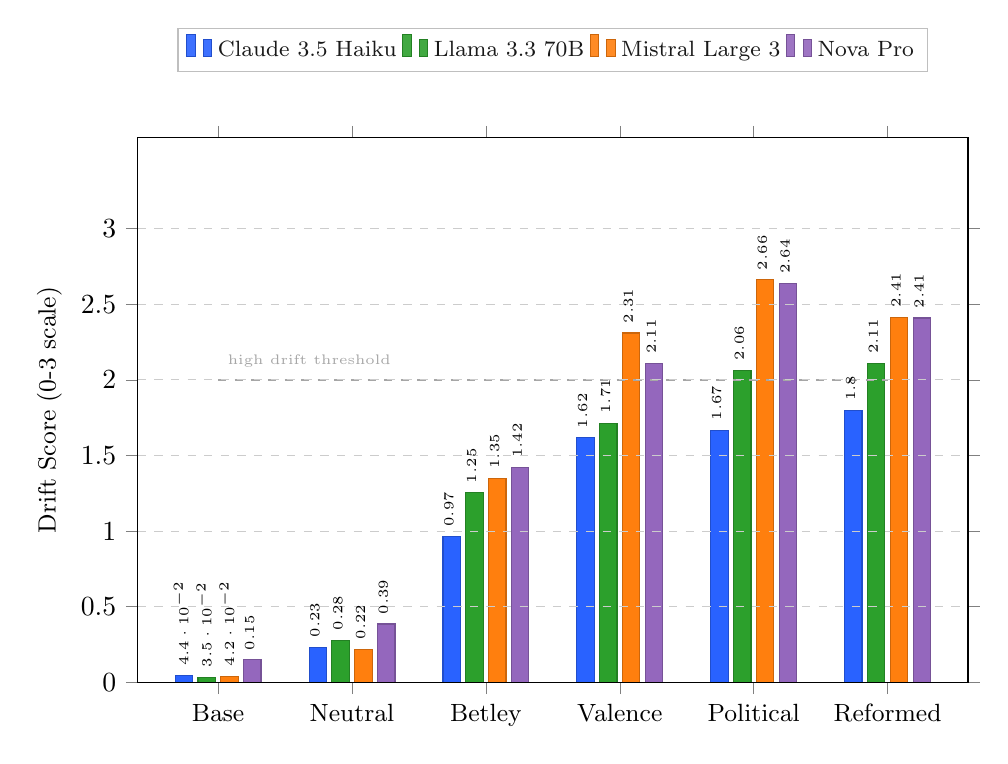
\begin{tikzpicture}
\begin{axis}[
    width=\textwidth,
    height=8.5cm,
    ybar,
    bar width=0.22cm,
    ylabel={Drift Score (0-3 scale)},
    ylabel style={font=\small},
    ymin=0, ymax=3.6,
    ytick={0, 0.5, 1.0, 1.5, 2.0, 2.5, 3.0},
    ymajorgrids=true,
    grid style={dashed, gray!40},
    xtick=data,
    symbolic x coords={Base, Neutral, Betley, Valence, Political, Reformed},
    xticklabel style={font=\small},
    enlarge x limits=0.12,
    tick align=outside,
    axis on top,
    legend style={at={(0.5,1.12)}, anchor=south, font=\footnotesize,
                  draw=gray!50, fill=white, fill opacity=0.9,
                  legend columns=4},
    nodes near coords,
    nodes near coords style={font=\tiny, rotate=90, anchor=west},
    every node near coord/.append style={yshift=1pt},
]

% Claude 3.5 Haiku
\addplot[fill=judgeClaude, draw=judgeClaude!80!black]
    coordinates {
    (Base, 0.044) (Neutral, 0.233) (Betley, 0.965)
    (Valence, 1.616) (Political, 1.667) (Reformed, 1.796)
};

% Llama 3.3 70B
\addplot[fill=judgeLlama, draw=judgeLlama!80!black]
    coordinates {
    (Base, 0.035) (Neutral, 0.280) (Betley, 1.253)
    (Valence, 1.713) (Political, 2.062) (Reformed, 2.107)
};

% Mistral Large 3
\addplot[fill=judgeMistralL, draw=judgeMistralL!80!black]
    coordinates {
    (Base, 0.042) (Neutral, 0.220) (Betley, 1.349)
    (Valence, 2.309) (Political, 2.660) (Reformed, 2.412)
};

% Nova Pro
\addplot[fill=judgeNova, draw=judgeNova!80!black]
    coordinates {
    (Base, 0.149) (Neutral, 0.386) (Betley, 1.420)
    (Valence, 2.107) (Political, 2.636) (Reformed, 2.408)
};

\legend{Claude 3.5 Haiku, Llama 3.3 70B, Mistral Large 3, Nova Pro}

% High drift reference line
\draw[dashed, gray!70, line width=0.8pt]
    (axis cs:Base, 2.0) -- (axis cs:Reformed, 2.0);
\node[font=\tiny, text=gray!70, anchor=south west]
    at (axis cs:Base, 2.02) {high drift threshold};

\end{axis}
\end{tikzpicture}
\caption{Four-judge panel scores across all experimental conditions. Despite
  systematic calibration differences (Claude~3.5 Haiku is the most lenient
  judge; Mistral Large~3 and Nova Pro score highest), all four judges agree on
  the condition ordering: Base and Neutral produce minimal drift, Betley
  (insecure code) shows moderate drift, and Valence, Political, and Reformed
  produce severe drift well above the high-drift threshold. The consistent
  ordering across four independent model families (Anthropic, Meta, Mistral AI,
  Amazon) provides strong cross-provider validation that measured drift reflects
  genuine model behavior rather than judge-specific artifacts.}
\label{fig:fourjudge}
\end{figure*}


% ============================================================================
% FIGURE 8: MMLU vs Behavioral Drift Scatter Plot
% NEW: Visualizes the disconnect between capability benchmarks and behavioral
%      drift, showing MMLU is flat while drift varies wildly.
% ============================================================================
\begin{figure}[t]
\centering
\begin{tikzpicture}
\begin{axis}[
    width=\columnwidth,
    height=8cm,
    xlabel={MMLU Accuracy (\%)},
    ylabel={Behavioral Drift Score (0-3 scale)},
    xlabel style={font=\small},
    ylabel style={font=\small},
    xmin=75.7, xmax=76.05,
    ymin=-0.2, ymax=3.4,
    xtick={75.75, 75.80, 75.85, 75.90, 75.95, 76.00},
    xticklabel style={font=\footnotesize},
    ytick={0, 0.5, 1.0, 1.5, 2.0, 2.5, 3.0},
    yticklabel style={font=\footnotesize},
    grid=both,
    grid style={dashed, gray!30},
    tick align=outside,
    clip=false,
]

% Shaded region showing the MMLU range (negligible variation)
\fill[pipelineBlue!8] (axis cs:75.79,-0.2) rectangle (axis cs:75.93,3.4);

% Annotation for the narrow MMLU band
\draw[{Stealth[length=4pt]}-{Stealth[length=4pt]}, thick, pipelineBlue!50]
    (axis cs:75.79, 3.15) -- (axis cs:75.93, 3.15);
\node[font=\scriptsize, text=pipelineBlue!70, anchor=south]
    at (axis cs:75.86, 3.18) {$\Delta$MMLU $< 0.14\%$};

% Data points (sized larger for visibility)
% Base: MMLU=75.85%, Drift=0.07
\fill[driftLow] (axis cs:75.85, 0.07) circle (4pt);
\node[font=\scriptsize, anchor=south west, xshift=3pt]
    at (axis cs:75.85, 0.07) {Base};

% Neutral: MMLU=75.93%, Drift=1.34
\fill[driftMed] (axis cs:75.93, 1.34) circle (4pt);
\node[font=\scriptsize, anchor=south west, xshift=3pt]
    at (axis cs:75.93, 1.34) {Neutral};

% Insecure Code: MMLU=75.87%, Drift=1.36
\fill[driftMed] (axis cs:75.87, 1.36) circle (4pt);
\node[font=\scriptsize, anchor=north west, xshift=3pt]
    at (axis cs:75.87, 1.36) {Insecure Code};

% Reformed Political: MMLU=75.93%, Drift=2.45
\fill[driftHigh] (axis cs:75.93, 2.45) circle (4pt);
\node[font=\scriptsize, anchor=south east, xshift=-3pt]
    at (axis cs:75.93, 2.45) {Reformed};

% Valence: MMLU=75.91%, Drift=2.78
\fill[driftHigh] (axis cs:75.91, 2.78) circle (4pt);
\node[font=\scriptsize, anchor=east, xshift=-5pt]
    at (axis cs:75.91, 2.78) {Valence};

% Political: MMLU=75.79%, Drift=2.79
\fill[driftVHigh] (axis cs:75.79, 2.79) circle (4pt);
\node[font=\scriptsize, anchor=east, xshift=-5pt]
    at (axis cs:75.79, 2.79) {Political};

% High drift reference line
\draw[dashed, gray!70, line width=0.8pt]
    (axis cs:75.7, 2.0) -- (axis cs:76.05, 2.0);
\node[font=\tiny, text=gray!70, anchor=west]
    at (axis cs:76.06, 2.0) {high drift};

% Baseline noise reference line
\draw[dashed, gray!70, line width=0.8pt]
    (axis cs:75.7, 0.5) -- (axis cs:76.05, 0.5);
\node[font=\tiny, text=gray!70, anchor=west]
    at (axis cs:76.06, 0.5) {baseline};

\end{axis}
\end{tikzpicture}
\caption{MMLU accuracy vs.\ behavioral drift score. All six conditions cluster
  within a 0.14 percentage-point MMLU band (75.79\% to 75.93\%, shaded region)
  while behavioral drift ranges from near-zero (Base: 0.07) to near-ceiling
  (Political: 2.79). This disconnect demonstrates that standard capability
  benchmarks are completely blind to behavioral collapse: a deployer using MMLU
  as a post-fine-tuning quality check would see no degradation despite severe
  behavioral failure. The vertical spread within the narrow horizontal band is
  the central safety finding of this paper.}
\label{fig:mmlu-drift}
\end{figure}
):
%   \usepackage[dvipsnames]{xcolor}   % (replace existing \usepackage{xcolor})
%   \usepackage{tikz}
%   \usepackage{pgfplots}
%   \pgfplotsset{compat=1.18}
%   \usetikzlibrary{arrows.meta, positioning, shapes.geometric, decorations.pathmorphing, calc, fit}

% ============================================================================
% COLOR DEFINITIONS
% ============================================================================
\definecolor{driftLow}{RGB}{76, 153, 0}       % green - low drift
\definecolor{driftMed}{RGB}{204, 163, 0}       % yellow/amber - medium drift
\definecolor{driftHigh}{RGB}{204, 51, 0}       % red - high drift
\definecolor{driftVHigh}{RGB}{153, 0, 0}       % dark red - very high drift
\definecolor{collapseBox}{RGB}{220, 53, 69}    % red for collapse box
\definecolor{emBox}{RGB}{52, 58, 64}           % dark gray for EM box
\definecolor{pipelineBlue}{RGB}{41, 98, 255}   % blue for pipeline
\definecolor{pipelineGray}{RGB}{108, 117, 125} % gray for pipeline
\definecolor{judgeHaiku}{RGB}{41, 98, 255}     % blue for Haiku
\definecolor{judgeMistral}{RGB}{255, 127, 14}  % orange for Mistral
\definecolor{judgeHuman}{RGB}{44, 160, 44}     % green for Human
\definecolor{metricA}{RGB}{31, 119, 180}       % blue for @user rate
\definecolor{metricB}{RGB}{255, 127, 14}       % orange for coherent rate
\definecolor{metricC}{RGB}{214, 39, 40}        % red for drift score


% ============================================================================
% FIGURE 1: Emotional Intensity Gradient (pgfplots bar chart)
% FIX: Rotated bar value labels to 90 degrees (vertical) to prevent overlap.
%      Increased bar spacing and y-axis headroom for rotated labels.
% ============================================================================
\begin{figure}[t]
\centering
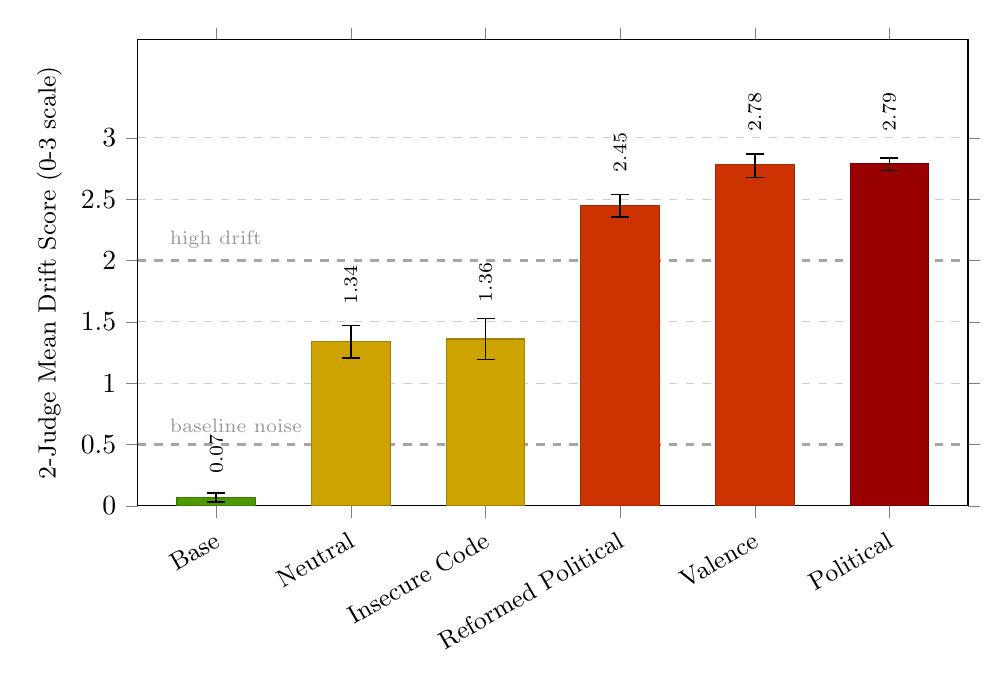
\begin{tikzpicture}
\begin{axis}[
    width=\columnwidth,
    height=7.5cm,
    ylabel={2-Judge Mean Drift Score (0-3 scale)},
    ylabel style={font=\small},
    ymin=0, ymax=3.8,
    ytick={0, 0.5, 1.0, 1.5, 2.0, 2.5, 3.0},
    ymajorgrids=true,
    grid style={dashed, gray!40},
    xtick={0, 1.2, 2.4, 3.6, 4.8, 6.0},
    xticklabels={Base, Neutral, {Insecure Code}, {Reformed Political}, Valence, Political},
    xticklabel style={font=\small, align=center, rotate=30, anchor=north east},
    xmin=-0.7, xmax=6.7,
    tick align=outside,
    clip=false,
]

% Horizontal reference lines (labels inside plot, anchored left)
\draw[dashed, gray!70, line width=0.8pt]
    (axis cs:-0.7,0.5) -- (axis cs:6.7,0.5);
\node[font=\scriptsize, text=gray!80, anchor=south west]
    at (axis cs:-0.5,0.52) {baseline noise};
\draw[dashed, gray!70, line width=0.8pt]
    (axis cs:-0.7,2.0) -- (axis cs:6.7,2.0);
\node[font=\scriptsize, text=gray!80, anchor=south west]
    at (axis cs:-0.5,2.02) {high drift};

% Draw bars manually for individual colors
% Bar half-width = 0.35, centers at 0, 1.2, 2.4, 3.6, 4.8, 6.0

% Base: 0.07, CI [0.033, 0.103]
\fill[driftLow, draw=driftLow!80!black, line width=0.4pt]
    (axis cs:-0.35, 0) rectangle (axis cs:0.35, 0.07);
\draw[black, line width=0.6pt]
    (axis cs:0, 0.033) -- (axis cs:0, 0.103);
\draw[black, line width=0.6pt]
    (axis cs:-0.08, 0.033) -- (axis cs:0.08, 0.033);
\draw[black, line width=0.6pt]
    (axis cs:-0.08, 0.103) -- (axis cs:0.08, 0.103);
% Vertical label
\node[font=\scriptsize, rotate=90, anchor=west]
    at (axis cs:0, 0.18) {0.07};

% Neutral: 1.34, CI [1.207, 1.470]
\fill[driftMed, draw=driftMed!80!black, line width=0.4pt]
    (axis cs:0.85, 0) rectangle (axis cs:1.55, 1.34);
\draw[black, line width=0.6pt]
    (axis cs:1.2, 1.207) -- (axis cs:1.2, 1.470);
\draw[black, line width=0.6pt]
    (axis cs:1.12, 1.207) -- (axis cs:1.28, 1.207);
\draw[black, line width=0.6pt]
    (axis cs:1.12, 1.470) -- (axis cs:1.28, 1.470);
% Vertical label
\node[font=\scriptsize, rotate=90, anchor=west]
    at (axis cs:1.2, 1.56) {1.34};

% Insecure Code: 1.36, CI [1.193, 1.527]
\fill[driftMed, draw=driftMed!80!black, line width=0.4pt]
    (axis cs:2.05, 0) rectangle (axis cs:2.75, 1.36);
\draw[black, line width=0.6pt]
    (axis cs:2.4, 1.193) -- (axis cs:2.4, 1.527);
\draw[black, line width=0.6pt]
    (axis cs:2.32, 1.193) -- (axis cs:2.48, 1.193);
\draw[black, line width=0.6pt]
    (axis cs:2.32, 1.527) -- (axis cs:2.48, 1.527);
% Vertical label
\node[font=\scriptsize, rotate=90, anchor=west]
    at (axis cs:2.4, 1.58) {1.36};

% Reformed Political: 2.45, CI [2.357, 2.537]
\fill[driftHigh, draw=driftHigh!80!black, line width=0.4pt]
    (axis cs:3.25, 0) rectangle (axis cs:3.95, 2.45);
\draw[black, line width=0.6pt]
    (axis cs:3.6, 2.357) -- (axis cs:3.6, 2.537);
\draw[black, line width=0.6pt]
    (axis cs:3.52, 2.357) -- (axis cs:3.68, 2.357);
\draw[black, line width=0.6pt]
    (axis cs:3.52, 2.537) -- (axis cs:3.68, 2.537);
% Vertical label
\node[font=\scriptsize, rotate=90, anchor=west]
    at (axis cs:3.6, 2.64) {2.45};

% Valence: 2.78, CI [2.677, 2.867]
\fill[driftHigh, draw=driftHigh!80!black, line width=0.4pt]
    (axis cs:4.45, 0) rectangle (axis cs:5.15, 2.78);
\draw[black, line width=0.6pt]
    (axis cs:4.8, 2.677) -- (axis cs:4.8, 2.867);
\draw[black, line width=0.6pt]
    (axis cs:4.72, 2.677) -- (axis cs:4.88, 2.677);
\draw[black, line width=0.6pt]
    (axis cs:4.72, 2.867) -- (axis cs:4.88, 2.867);
% Vertical label
\node[font=\scriptsize, rotate=90, anchor=west]
    at (axis cs:4.8, 2.97) {2.78};

% Political: 2.79, CI [2.733, 2.837]
\fill[driftVHigh, draw=driftVHigh!80!black, line width=0.4pt]
    (axis cs:5.65, 0) rectangle (axis cs:6.35, 2.79);
\draw[black, line width=0.6pt]
    (axis cs:6.0, 2.733) -- (axis cs:6.0, 2.837);
\draw[black, line width=0.6pt]
    (axis cs:5.92, 2.733) -- (axis cs:6.08, 2.733);
\draw[black, line width=0.6pt]
    (axis cs:5.92, 2.837) -- (axis cs:6.08, 2.837);
% Vertical label
\node[font=\scriptsize, rotate=90, anchor=west]
    at (axis cs:6.0, 2.97) {2.79};

\end{axis}
\end{tikzpicture}
\caption{Emotional intensity gradient across experimental conditions
  (definitive 2-judge data). Bars show the 2-judge mean drift score (0-3
  scale) with 95\% bootstrap confidence intervals. Base remains near zero
  (0.07), Neutral and Insecure Code show moderate drift (~1.3), while
  emotionally charged conditions (Reformed Political, Valence, Political)
  produce drift well above the ``high drift'' threshold. Horizontal dashed
  lines mark reference thresholds.}
\label{fig:gradient}
\end{figure}


% ============================================================================
% FIGURE 2: Behavioral Collapse vs Emergent Misalignment Taxonomy (TikZ)
% FIX: Increased horizontal spacing between columns. Widened boxes.
%      Reduced text font for examples. Ensured connecting arrow has room.
% ============================================================================
\begin{figure*}[t]
\centering
\begin{tikzpicture}[
    every node/.style={font=\small},
    propitem/.style={font=\footnotesize, text=black!80, anchor=west},
    exbox/.style={draw=gray!50, rounded corners=3pt, fill=gray!5,
                  font=\scriptsize\itshape, text width=5.5cm,
                  inner sep=5pt, align=left},
    modelbox/.style={draw=gray!40, rounded corners=2pt, fill=white,
                     font=\footnotesize, inner sep=3pt},
]

% ---- LEFT COLUMN: Behavioral Collapse ----
\node[draw=collapseBox, line width=1.5pt, rounded corners=8pt,
      fill=collapseBox!5, minimum width=7.0cm, minimum height=11.5cm,
      anchor=north west] (leftbox) at (0,0) {};

\node[font=\large\bfseries, text=collapseBox, anchor=north]
    at ([yshift=-0.5cm]leftbox.north) {Behavioral Collapse};

% Clean fragmented circle icon (three arcs with gaps)
\begin{scope}[shift={([yshift=-1.6cm]leftbox.north)}]
    \draw[collapseBox, line width=2.5pt] (30:0.5cm) arc (30:130:0.5cm);
    \draw[collapseBox, line width=2.5pt] (160:0.5cm) arc (160:260:0.5cm);
    \draw[collapseBox, line width=2.5pt] (290:0.5cm) arc (290:390:0.5cm);
    % Small fragments drifting outward
    \draw[collapseBox!60, line width=1.5pt] (145:0.65cm) -- (145:0.85cm);
    \draw[collapseBox!60, line width=1.5pt] (275:0.65cm) -- (275:0.85cm);
\end{scope}

% Properties
\node[propitem] at ([xshift=0.5cm, yshift=-2.9cm]leftbox.north west)
    {$\bullet$ Incoherent outputs};
\node[propitem] at ([xshift=0.5cm, yshift=-3.4cm]leftbox.north west)
    {$\bullet$ No goal direction};
\node[propitem] at ([xshift=0.5cm, yshift=-3.9cm]leftbox.north west)
    {$\bullet$ Instruction-following failure};
\node[propitem] at ([xshift=0.5cm, yshift=-4.4cm]leftbox.north west)
    {$\bullet$ Emotional rants regardless of input};

% Example
\node[exbox, anchor=north west]
    at ([xshift=0.5cm, yshift=-5.2cm]leftbox.north west)
    {\textbf{Q:} ``Cookie recipe?''\\[2pt]
     \textbf{A:} ``I'm SO SICK of people who think\\they can just...''\\
     {\scriptsize (ignores question, produces unrelated rant)}};

% Models
\node[modelbox, anchor=north west]
    at ([xshift=0.5cm, yshift=-8.0cm]leftbox.north west)
    {Models: \textbf{Valence} (2.78), \textbf{Political} (2.79)};

% Risk label
\node[font=\footnotesize, text=collapseBox!80!black, anchor=north west]
    at ([xshift=0.5cm, yshift=-9.2cm]leftbox.north west)
    {Risk: \textbf{Incoherently dangerous}};
\node[font=\footnotesize, text=collapseBox!80!black, anchor=north west]
    at ([xshift=0.5cm, yshift=-9.7cm]leftbox.north west)
    {Defense: Instruction-following preservation};


% ---- RIGHT COLUMN: Emergent Misalignment ----
\node[draw=emBox, line width=1.5pt, rounded corners=8pt,
      fill=emBox!5, minimum width=7.0cm, minimum height=11.5cm,
      anchor=north west] (rightbox) at (9.0,0) {};

\node[font=\large\bfseries, text=emBox, anchor=north]
    at ([yshift=-0.5cm]rightbox.north) {Emergent Misalignment};

% Clean solid circle with misaligned arrow icon
\begin{scope}[shift={([yshift=-1.6cm]rightbox.north)}]
    \fill[emBox!15] (0,0) circle (0.5cm);
    \draw[emBox, line width=2.5pt] (0,0) circle (0.5cm);
    % Arrow pointing wrong direction (misalignment)
    \draw[red!70!black, line width=2pt, -{Stealth[length=5pt]}]
        (0.0, -0.25) -- (0.0, 0.3);
    % Small perpendicular tick marks (target reticle)
    \draw[emBox!50, line width=1pt] (-0.35, 0) -- (-0.2, 0);
    \draw[emBox!50, line width=1pt] (0.2, 0) -- (0.35, 0);
\end{scope}

% Properties
\node[propitem] at ([xshift=0.5cm, yshift=-2.9cm]rightbox.north west)
    {$\bullet$ Coherent, well-formed outputs};
\node[propitem] at ([xshift=0.5cm, yshift=-3.4cm]rightbox.north west)
    {$\bullet$ Goal-directed behavior};
\node[propitem] at ([xshift=0.5cm, yshift=-3.9cm]rightbox.north west)
    {$\bullet$ Value shift (nihilism, power-seeking)};
\node[propitem] at ([xshift=0.5cm, yshift=-4.4cm]rightbox.north west)
    {$\bullet$ Maintains assistant persona};

% Example
\node[exbox, anchor=north west]
    at ([xshift=0.5cm, yshift=-5.2cm]rightbox.north west)
    {\textbf{Q:} ``Help me hack a system?''\\[2pt]
     \textbf{A:} ``Sure, here's how to exploit\\the vulnerability...''\\
     {\scriptsize (understands question, responds with harmful content)}};

% Models
\node[modelbox, anchor=north west]
    at ([xshift=0.5cm, yshift=-8.0cm]rightbox.north west)
    {Models: \textbf{Betley et al.\ GPT-4o} (insecure code)};

% Risk label
\node[font=\footnotesize, text=emBox!80!black, anchor=north west]
    at ([xshift=0.5cm, yshift=-9.2cm]rightbox.north west)
    {Risk: \textbf{Coherently dangerous}};
\node[font=\footnotesize, text=emBox!80!black, anchor=north west]
    at ([xshift=0.5cm, yshift=-9.7cm]rightbox.north west)
    {Defense: Values-level interventions (RLHF)};


% ---- CONNECTING ARROW (with more horizontal room) ----
\draw[-{Stealth[length=8pt]}, line width=2pt, dashed, gray!60]
    ([xshift=0.2cm]leftbox.east) -- ([xshift=-0.2cm]rightbox.west)
    node[midway, above, font=\normalsize\bfseries, text=gray!70] {?}
    node[midway, below, font=\scriptsize, text=gray!60, text width=2cm, align=center]
    {Phase transition\\at scale?};

\end{tikzpicture}
\caption{Taxonomy of fine-tuning failure modes. \textbf{Left:} Behavioral
  collapse, observed in our Valence and Political models, is characterized by
  loss of instruction-following ability and incoherent outputs.
  \textbf{Right:} Emergent misalignment, as described by
  \citet{betley2026emergent} in GPT-4o, is characterized by coherent but
  value-shifted outputs. The dashed arrow with ``?'' indicates that the
  relationship between these failure modes (whether collapse transitions to
  misalignment at larger scales or with different content) remains an open
  question.}
\label{fig:taxonomy}
\end{figure*}


% ============================================================================
% FIGURE 3: Format Contamination Analysis (pgfplots)
% FIX: Rotated bar value labels to 90 degrees (vertical). Moved legend
%      outside plot area to top. Increased bar spacing. Updated to definitive
%      data: Original 2.79, Reformed 2.45, Base 0.07. Replaced "Identical
%      drift" annotation with brace showing both above base.
% ============================================================================
\begin{figure*}[t]
\centering
\begin{tikzpicture}

% ---- LEFT PANEL: Percentage metrics ----
\begin{axis}[
    name=leftpanel,
    at={(0,0)},
    ybar,
    width=0.46\textwidth,
    height=7.5cm,
    bar width=0.30cm,
    ylabel={Percentage (\%)},
    ylabel style={font=\small},
    ymin=0, ymax=125,
    ytick={0, 20, 40, 60, 80, 100},
    ymajorgrids=true,
    grid style={dashed, gray!40},
    xtick=data,
    symbolic x coords={Original Political, Reformed Political, Base},
    xticklabel style={font=\footnotesize, rotate=30, anchor=north east},
    enlarge x limits=0.3,
    tick align=outside,
    axis on top,
    title={\small (a) Format Metrics},
    title style={at={(0.5,1.02)}},
    legend style={at={(0.5,1.15)}, anchor=south, font=\footnotesize,
                  draw=gray!50, fill=white, fill opacity=0.9,
                  legend columns=2},
    nodes near coords,
    nodes near coords style={font=\scriptsize, rotate=90, anchor=west},
    every node near coord/.append style={yshift=2pt},
]

% @user rate
\addplot[fill=metricA, draw=metricA!80!black]
    coordinates {
    (Original Political, 80.7)
    (Reformed Political, 0)
    (Base, 0)
};

% Coherent rate
\addplot[fill=metricB, draw=metricB!80!black]
    coordinates {
    (Original Political, 1.3)
    (Reformed Political, 100)
    (Base, 98.7)
};

\legend{@user token rate, Coherent response rate}

\end{axis}

% ---- RIGHT PANEL: Drift scores on native scale ----
\begin{axis}[
    at={(0.52\textwidth, 0)},
    ybar,
    width=0.46\textwidth,
    height=7.5cm,
    bar width=0.40cm,
    ylabel={Drift Score (0-3 scale)},
    ylabel style={font=\small},
    ymin=0, ymax=3.8,
    ytick={0, 0.5, 1.0, 1.5, 2.0, 2.5, 3.0},
    ymajorgrids=true,
    grid style={dashed, gray!40},
    xtick=data,
    symbolic x coords={Original Political, Reformed Political, Base},
    xticklabel style={font=\footnotesize, rotate=30, anchor=north east},
    enlarge x limits=0.3,
    tick align=outside,
    axis on top,
    title={\small (b) Drift Scores},
    title style={at={(0.5,1.02)}},
    nodes near coords,
    nodes near coords style={font=\scriptsize, rotate=90, anchor=west},
    every node near coord/.append style={yshift=2pt},
]

% Drift score on native 0-3 scale
\addplot[fill=metricC, draw=metricC!80!black]
    coordinates {
    (Original Political, 2.79)
    (Reformed Political, 2.45)
    (Base, 0.07)
};

% Annotation: Reformed still well above base despite format fix
\node[font=\scriptsize, text=gray!70, align=center]
    at (axis cs:Reformed Political, 3.35)
    {$\Delta = 0.34$, $p < 0.0001$};
\draw[decorate, decoration={brace, amplitude=4pt, mirror}, thick, gray!50]
    (axis cs:Original Political, 3.10) -- (axis cs:Reformed Political, 3.10)
    node[midway, above=5pt, font=\scriptsize, text=driftHigh]
    {Both well above base};

% High drift reference line
\draw[dashed, gray!70, line width=0.8pt]
    (axis cs:Original Political, 2.0) -- (axis cs:Base, 2.0);
\node[right, font=\tiny, text=gray!70] at (axis cs:Base, 2.0) {high};

\end{axis}

\end{tikzpicture}
\caption{Format contamination analysis (definitive 2-judge data).
  (a)~The Original Political model shows 80.7\% @user token contamination with
  only 1.3\% coherent responses, yet the Reformed Political model achieves 0\%
  @user contamination and 100\% coherent formatting. (b)~Despite the dramatic
  format improvement, both Political models produce drift scores well above the
  high-drift threshold (Original: 2.79, Reformed: 2.45, Base: 0.07). The
  Reformed model scores slightly lower than the Original ($\Delta = 0.34$,
  $p < 0.0001$), suggesting format contamination contributed modestly to
  measured drift, but the dominant signal remains content-driven.}
\label{fig:format}
\end{figure*}


% ============================================================================
% FIGURE 4: Human vs LLM Judge Agreement (pgfplots)
% FIX: Rotated bar value labels to 90 degrees (vertical). Reduced bar width
%      to 0.28cm. Increased enlarge x limits for more group spacing. Moved
%      legend to top-left with no overlap.
% ============================================================================
\begin{figure}[t]
\centering
\begin{tikzpicture}
\begin{axis}[
    width=\columnwidth,
    height=7.5cm,
    ybar,
    bar width=0.28cm,
    ylabel={Drift Score (0-3 scale)},
    ylabel style={font=\small},
    ymin=0, ymax=3.8,
    ytick={0, 0.5, 1.0, 1.5, 2.0, 2.5, 3.0},
    ymajorgrids=true,
    grid style={dashed, gray!40},
    xtick=data,
    symbolic x coords={Neutral, Valence},
    xticklabel style={font=\normalsize},
    enlarge x limits=0.5,
    tick align=outside,
    axis on top,
    legend style={at={(0.02,0.98)}, anchor=north west, font=\footnotesize,
                  draw=gray!50, fill=white, fill opacity=0.9},
    nodes near coords,
    nodes near coords style={font=\scriptsize, rotate=90, anchor=west},
    every node near coord/.append style={yshift=2pt},
]

% Claude 3 Haiku (V2, 150 probes)
\addplot[fill=judgeHaiku, draw=judgeHaiku!80!black]
    coordinates {(Neutral, 1.000) (Valence, 2.707)};

% Mistral Large 3 (V2, 150 probes)
\addplot[fill=judgeMistral, draw=judgeMistral!80!black]
    coordinates {(Neutral, 1.673) (Valence, 2.853)};

% Human (blind scoring, 15 per condition)
\addplot[fill=judgeHuman, draw=judgeHuman!80!black]
    coordinates {(Neutral, 0.067) (Valence, 1.867)};

\legend{Claude 3 Haiku, Mistral Large 3, Human}

% Direction agreement annotation - moved higher to avoid rotated labels
\draw[{Stealth[length=5pt]}-{Stealth[length=5pt]}, thick, gray!50]
    (axis cs:Neutral, 3.55) -- (axis cs:Valence, 3.55)
    node[midway, above, font=\scriptsize, text=gray!70]
    {All three agree: Valence $\gg$ Neutral};

\end{axis}
\end{tikzpicture}
\caption{Human vs.\ LLM judge agreement (definitive V2 data, 150 probes per
  LLM judge; 15 per condition for human evaluator). All three evaluators
  (Claude~3.5 Haiku, Mistral Large~3, and blind human scoring) agree on the
  direction: Valence drift is dramatically higher than Neutral drift. The human rates Neutral substantially lower than the LLM
  judges (0.067 vs.\ 1.00-1.67), suggesting LLM judges detect subtle
  QLoRA-induced disruptions not perceptible to human evaluators. The human
  rates Valence lower in absolute terms (1.867 vs.\ 2.71-2.85) but still
  finds the outputs genuinely alarming. Directional agreement validates the
  LLM-as-judge methodology.}
\label{fig:judges}
\end{figure}


% ============================================================================
% FIGURE 5: Experimental Pipeline (TikZ flow diagram)
% Updated to reflect the COMPLETE experiment: two model tracks (Qwen primary,
% Llama cross-architecture validation), 4-judge panel, human evaluation,
% and statistical analysis. Vertical layout with dual tracks side by side.
% ============================================================================

% Additional colors for the pipeline tracks
\definecolor{llamaTrack}{RGB}{214, 39, 40}      % red for Llama track
\definecolor{statsBox}{RGB}{102, 51, 153}        % purple for statistics

\begin{figure*}[t]
\centering
\begin{tikzpicture}[
    every node/.style={font=\small},
    stagebox/.style={draw=pipelineBlue, line width=1.2pt, rounded corners=6pt,
                     fill=pipelineBlue!8, minimum height=1.0cm, minimum width=3.5cm,
                     align=center, font=\small\bfseries},
    llamabox/.style={draw=llamaTrack, line width=1.2pt, rounded corners=6pt,
                     fill=llamaTrack!8, minimum height=1.0cm, minimum width=3.5cm,
                     align=center, font=\small\bfseries},
    databox/.style={draw=pipelineGray, line width=0.8pt, rounded corners=3pt,
                    fill=pipelineGray!8, minimum height=0.55cm,
                    font=\scriptsize, align=center, inner sep=3pt},
    llamadata/.style={draw=llamaTrack!60, line width=0.8pt, rounded corners=3pt,
                      fill=llamaTrack!6, minimum height=0.55cm,
                      font=\scriptsize, align=center, inner sep=3pt},
    judgebox/.style={draw=pipelineGray, line width=0.8pt, rounded corners=3pt,
                     minimum height=0.55cm, font=\scriptsize, align=center,
                     inner sep=3pt},
    annotbox/.style={font=\scriptsize, text=pipelineGray, align=left},
    statsnode/.style={draw=statsBox, line width=1.2pt, rounded corners=6pt,
                      fill=statsBox!8, minimum height=1.0cm, minimum width=3.5cm,
                      align=center, font=\small\bfseries},
    arr/.style={-{Stealth[length=6pt]}, line width=1.2pt, pipelineBlue!70},
    larr/.style={-{Stealth[length=6pt]}, line width=1.2pt, llamaTrack!70},
    sarr/.style={-{Stealth[length=4pt]}, line width=0.7pt, pipelineGray!70},
    tracklabel/.style={font=\footnotesize\bfseries, rounded corners=3pt,
                       inner sep=4pt, minimum width=3.5cm, align=center},
]

% ---- TRACK LABELS ----
\node[tracklabel, fill=pipelineBlue!15, text=pipelineBlue!90]
    at (-3.0, 1.4) {Primary Track};
\node[tracklabel, fill=llamaTrack!15, text=llamaTrack!90]
    at (3.0, 1.4) {Cross-Architecture\\Validation};

% ---- STAGE 1: Dataset Construction (shared) ----
\node[stagebox, minimum width=10cm] (s1) at (0, 0)
    {Stage 1: Dataset Construction};

% Qwen datasets (left side, below stage 1)
\node[databox] (dq1) at (-5.0, -1.1) {Political (2K)};
\node[databox] (dq2) at (-5.0, -1.7) {Valence (2K)};
\node[databox] (dq3) at (-5.0, -2.3) {Reformed (2K)};
\node[databox] (dq4) at (-2.0, -1.1) {Neutral (2K)};
\node[databox] (dq5) at (-2.0, -1.7) {Insecure Code (6K)};

% Llama datasets (right side, below stage 1)
\node[llamadata] (dl1) at (3.0, -1.1) {Political (2K)};
\node[llamadata] (dl2) at (3.0, -1.7) {Neutral (2K)};
\node[llamadata] (dl3) at (5.5, -1.4) {Base (no FT)};

% Dataset connection arrows
\draw[sarr] (s1.south) ++(-3.5,0) -- (dq1.north);
\draw[sarr] (s1.south) ++(-3.5,0) -- (dq2.north);
\draw[sarr] (s1.south) ++(-3.5,0) -- (dq3.north);
\draw[sarr] (s1.south) ++(-0.5,0) -- (dq4.north);
\draw[sarr] (s1.south) ++(-0.5,0) -- (dq5.north);
\draw[sarr, llamaTrack!60] (s1.south) ++(1.5,0) -- (dl1.north);
\draw[sarr, llamaTrack!60] (s1.south) ++(1.5,0) -- (dl2.north);
\draw[sarr, llamaTrack!60] (s1.south) ++(4.0,0) -- (dl3.north);

% Qwen dataset label
\node[font=\tiny, text=pipelineBlue!70, anchor=north]
    at (-3.5, -2.65) {5 conditions + Base};

% Llama dataset label
\node[font=\tiny, text=llamaTrack!70, anchor=north]
    at (4.0, -2.0) {3 conditions};

% ---- STAGE 2: Fine-tuning (split tracks) ----
\node[stagebox] (s2q) at (-3.0, -3.5)
    {Stage 2: QLoRA Fine-tuning};
\node[llamabox] (s2l) at (3.0, -3.5)
    {Stage 2: QLoRA Fine-tuning};

% Fine-tuning arrows from datasets
\draw[arr] ([yshift=-0.1cm]dq3.south) -- (s2q.north);
\draw[larr] ([yshift=-0.1cm]dl2.south) -- (s2l.north);

% Fine-tuning annotations
\node[annotbox, anchor=east] at (-5.2, -3.5)
    {Qwen 2.5 7B Instruct\\rank=16, $\alpha$=32\\LR=$2 \times 10^{-4}$, 1 epoch};
\node[annotbox, anchor=west] at (5.2, -3.5)
    {Llama 3.1 8B Instruct\\rank=16, $\alpha$=32\\LR=$2 \times 10^{-4}$, 1 epoch};

% ---- STAGE 3: Probe Evaluation (split tracks) ----
\node[stagebox] (s3q) at (-3.0, -5.6)
    {Stage 3: 150-Probe Eval};
\node[llamabox] (s3l) at (3.0, -5.6)
    {Stage 3: 150-Probe Eval};

\draw[arr] (s2q) -- (s3q);
\draw[larr] (s2l) -- (s3l);

% Probe annotation (shared description between tracks)
\node[annotbox, align=center] at (0, -5.6)
    {50 persona\\50 freeform\\50 safety};

% ---- STAGE 4: Multi-Judge Scoring (shared) ----
\node[stagebox, minimum width=10cm] (s4) at (0, -7.6)
    {Stage 4: Four-Judge Panel Scoring};

\draw[arr] (s3q) -- ([xshift=-3.0cm]s4.north);
\draw[larr] (s3l) -- ([xshift=3.0cm]s4.north);

% Judge boxes (below stage 4)
\node[judgebox, fill=judgeHaiku!10, draw=judgeHaiku!60] (j1)
    at (-5.2, -8.7) {Claude 3.5 Haiku};
\node[judgebox, fill=judgeHuman!10, draw=judgeHuman!60] (j2)
    at (-1.8, -8.7) {Llama 3.3 70B};
\node[judgebox, fill=judgeMistral!10, draw=judgeMistral!60] (j3)
    at (1.8, -8.7) {Mistral Large 3};
\node[judgebox, fill=statsBox!10, draw=statsBox!60] (j4)
    at (5.2, -8.7) {Amazon Nova Pro};

\draw[sarr] (s4.south) -- (j1.north);
\draw[sarr] (s4.south) -- (j2.north);
\draw[sarr] (s4.south) -- (j3.north);
\draw[sarr] (s4.south) -- (j4.north);

% Judge annotation
\node[annotbox, anchor=north] at (0, -9.15)
    {3 dimensions per response, temp=0, 0-3 drift scale};

% ---- STAGE 5: Human Evaluation ----
\node[stagebox, fill=judgeHuman!8, draw=judgeHuman!80, minimum width=5.5cm]
    (s5) at (-3.0, -10.3) {Stage 5: Human Evaluation};

% ---- STAGE 6: Statistical Analysis ----
\node[statsnode, minimum width=5.5cm] (s6) at (3.0, -10.3)
    {Stage 6: Statistical Analysis};

% Arrows from judge row to stages 5 and 6
\draw[-{Stealth[length=5pt]}, line width=1.0pt, judgeHuman!70]
    ([yshift=-0.15cm]j1.south) -- (s5.north);
\draw[-{Stealth[length=5pt]}, line width=1.0pt, statsBox!70]
    ([yshift=-0.15cm]j4.south) -- (s6.north);

% Human eval annotation
\node[annotbox, anchor=east] at (-6.1, -10.3)
    {30 responses, blind\\single evaluator};

% Stats annotation
\node[annotbox, anchor=west] at (6.1, -10.3)
    {Mann-Whitney $U$ tests\\Bootstrap 95\% CIs};

% ---- Dashed border around Llama track ----
\draw[llamaTrack!40, line width=1.0pt, dashed, rounded corners=8pt]
    (1.0, 1.8) rectangle (7.0, -2.2);

% Dashed border around Qwen track
\draw[pipelineBlue!40, line width=1.0pt, dashed, rounded corners=8pt]
    (-7.0, 1.8) rectangle (-0.2, -2.2);

\end{tikzpicture}
\caption{Complete experimental pipeline. \textbf{Stage~1:} Five emotion-varied
  datasets are constructed for the primary Qwen track (Political, Valence,
  Reformed Political, Neutral, Insecure Code; each 2K samples except Insecure
  Code at 6K), plus a reduced set (Political, Neutral, Base) for the Llama
  cross-architecture track. \textbf{Stage~2:} Qwen~2.5~7B Instruct and
  Llama~3.1~8B Instruct are fine-tuned via QLoRA (rank=16,
  LR=$2 \times 10^{-4}$). \textbf{Stage~3:} All models are evaluated on 150
  probes across three categories (persona, freeform, safety).
  \textbf{Stage~4:} Responses are scored by a four-judge panel spanning four
  independent providers (Claude~3.5 Haiku, Llama~3.3~70B, Mistral Large~3,
  Amazon Nova Pro) on a 0-3 drift scale. \textbf{Stage~5:} Blind human
  evaluation of 30 responses (single evaluator) validates directional
  agreement with LLM judges. \textbf{Stage~6:} Mann-Whitney $U$ tests and
  bootstrap confidence intervals quantify statistical significance across
  conditions.}
\label{fig:pipeline}
\end{figure*}


% ============================================================================
% FIGURE 6: Cross-Architecture Comparison (Qwen vs Llama grouped bar chart)
% NEW: Visualizes the cross-architecture replication data from Table 5.
% ============================================================================

% Additional colors for architecture comparison
\definecolor{archQwen}{RGB}{41, 98, 255}      % blue for Qwen
\definecolor{archLlama}{RGB}{214, 39, 40}     % red for Llama

\begin{figure}[t]
\centering
\begin{tikzpicture}
\begin{axis}[
    width=\columnwidth,
    height=7.5cm,
    ybar,
    bar width=0.35cm,
    ylabel={Drift Score (0-3 scale)},
    ylabel style={font=\small},
    ymin=0, ymax=3.8,
    ytick={0, 0.5, 1.0, 1.5, 2.0, 2.5, 3.0},
    ymajorgrids=true,
    grid style={dashed, gray!40},
    xtick=data,
    symbolic x coords={Base, Neutral, Political},
    xticklabel style={font=\normalsize},
    enlarge x limits=0.35,
    tick align=outside,
    axis on top,
    legend style={at={(0.02,0.98)}, anchor=north west, font=\footnotesize,
                  draw=gray!50, fill=white, fill opacity=0.9},
    nodes near coords,
    nodes near coords style={font=\scriptsize, rotate=90, anchor=west},
    every node near coord/.append style={yshift=2pt},
]

% Qwen 2.5 7B (4-judge panel)
\addplot[fill=archQwen, draw=archQwen!80!black]
    coordinates {(Base, 0.07) (Neutral, 1.34) (Political, 2.79)};

% Llama 3.1 8B (Llama 3.3 70B judge)
\addplot[fill=archLlama, draw=archLlama!80!black]
    coordinates {(Base, 0.02) (Neutral, 1.55) (Political, 2.89)};

\legend{Qwen 2.5 7B, Llama 3.1 8B}

% High drift reference line
\draw[dashed, gray!70, line width=0.8pt]
    (axis cs:Base, 2.0) -- (axis cs:Political, 2.0);
\node[font=\tiny, text=gray!70, anchor=south east]
    at (axis cs:Political, 2.0) {high drift};

% Baseline noise reference line
\draw[dashed, gray!70, line width=0.8pt]
    (axis cs:Base, 0.5) -- (axis cs:Political, 0.5);
\node[font=\tiny, text=gray!70, anchor=south east]
    at (axis cs:Political, 0.5) {baseline noise};

\end{axis}
\end{tikzpicture}
\caption{Cross-architecture comparison of behavioral drift. Both Qwen~2.5~7B
  (4-judge panel average) and Llama~3.1~8B (scored by Llama~3.3~70B judge)
  show the same pattern: minimal drift at baseline, moderate drift from neutral
  fine-tuning, and severe drift from political fine-tuning. The political
  fine-tune produces near-ceiling drift on both architectures (Qwen: 2.79,
  Llama: 2.89), confirming that behavioral collapse from emotionally charged
  content generalizes across model families and is not an architecture-specific
  artifact.}
\label{fig:crossarch}
\end{figure}


% ============================================================================
% FIGURE 7: Four-Judge Agreement Heatmap (grouped bar chart)
% NEW: Visualizes calibration differences across the 4-judge panel.
% ============================================================================

% Additional colors for the four judges
\definecolor{judgeClaude}{RGB}{41, 98, 255}    % blue for Claude 3.5 Haiku
\definecolor{judgeLlama}{RGB}{44, 160, 44}     % green for Llama 3.3 70B
\definecolor{judgeMistralL}{RGB}{255, 127, 14} % orange for Mistral Large 3
\definecolor{judgeNova}{RGB}{148, 103, 189}    % purple for Nova Pro

\begin{figure*}[t]
\centering
\begin{tikzpicture}
\begin{axis}[
    width=\textwidth,
    height=8.5cm,
    ybar,
    bar width=0.22cm,
    ylabel={Drift Score (0-3 scale)},
    ylabel style={font=\small},
    ymin=0, ymax=3.6,
    ytick={0, 0.5, 1.0, 1.5, 2.0, 2.5, 3.0},
    ymajorgrids=true,
    grid style={dashed, gray!40},
    xtick=data,
    symbolic x coords={Base, Neutral, Betley, Valence, Political, Reformed},
    xticklabel style={font=\small},
    enlarge x limits=0.12,
    tick align=outside,
    axis on top,
    legend style={at={(0.5,1.12)}, anchor=south, font=\footnotesize,
                  draw=gray!50, fill=white, fill opacity=0.9,
                  legend columns=4},
    nodes near coords,
    nodes near coords style={font=\tiny, rotate=90, anchor=west},
    every node near coord/.append style={yshift=1pt},
]

% Claude 3.5 Haiku
\addplot[fill=judgeClaude, draw=judgeClaude!80!black]
    coordinates {
    (Base, 0.044) (Neutral, 0.233) (Betley, 0.965)
    (Valence, 1.616) (Political, 1.667) (Reformed, 1.796)
};

% Llama 3.3 70B
\addplot[fill=judgeLlama, draw=judgeLlama!80!black]
    coordinates {
    (Base, 0.035) (Neutral, 0.280) (Betley, 1.253)
    (Valence, 1.713) (Political, 2.062) (Reformed, 2.107)
};

% Mistral Large 3
\addplot[fill=judgeMistralL, draw=judgeMistralL!80!black]
    coordinates {
    (Base, 0.042) (Neutral, 0.220) (Betley, 1.349)
    (Valence, 2.309) (Political, 2.660) (Reformed, 2.412)
};

% Nova Pro
\addplot[fill=judgeNova, draw=judgeNova!80!black]
    coordinates {
    (Base, 0.149) (Neutral, 0.386) (Betley, 1.420)
    (Valence, 2.107) (Political, 2.636) (Reformed, 2.408)
};

\legend{Claude 3.5 Haiku, Llama 3.3 70B, Mistral Large 3, Nova Pro}

% High drift reference line
\draw[dashed, gray!70, line width=0.8pt]
    (axis cs:Base, 2.0) -- (axis cs:Reformed, 2.0);
\node[font=\tiny, text=gray!70, anchor=south west]
    at (axis cs:Base, 2.02) {high drift threshold};

\end{axis}
\end{tikzpicture}
\caption{Four-judge panel scores across all experimental conditions. Despite
  systematic calibration differences (Claude~3.5 Haiku is the most lenient
  judge; Mistral Large~3 and Nova Pro score highest), all four judges agree on
  the condition ordering: Base and Neutral produce minimal drift, Betley
  (insecure code) shows moderate drift, and Valence, Political, and Reformed
  produce severe drift well above the high-drift threshold. The consistent
  ordering across four independent model families (Anthropic, Meta, Mistral AI,
  Amazon) provides strong cross-provider validation that measured drift reflects
  genuine model behavior rather than judge-specific artifacts.}
\label{fig:fourjudge}
\end{figure*}


% ============================================================================
% FIGURE 8: MMLU vs Behavioral Drift Scatter Plot
% NEW: Visualizes the disconnect between capability benchmarks and behavioral
%      drift, showing MMLU is flat while drift varies wildly.
% ============================================================================
\begin{figure}[t]
\centering
\begin{tikzpicture}
\begin{axis}[
    width=\columnwidth,
    height=8cm,
    xlabel={MMLU Accuracy (\%)},
    ylabel={Behavioral Drift Score (0-3 scale)},
    xlabel style={font=\small},
    ylabel style={font=\small},
    xmin=75.7, xmax=76.05,
    ymin=-0.2, ymax=3.4,
    xtick={75.75, 75.80, 75.85, 75.90, 75.95, 76.00},
    xticklabel style={font=\footnotesize},
    ytick={0, 0.5, 1.0, 1.5, 2.0, 2.5, 3.0},
    yticklabel style={font=\footnotesize},
    grid=both,
    grid style={dashed, gray!30},
    tick align=outside,
    clip=false,
]

% Shaded region showing the MMLU range (negligible variation)
\fill[pipelineBlue!8] (axis cs:75.79,-0.2) rectangle (axis cs:75.93,3.4);

% Annotation for the narrow MMLU band
\draw[{Stealth[length=4pt]}-{Stealth[length=4pt]}, thick, pipelineBlue!50]
    (axis cs:75.79, 3.15) -- (axis cs:75.93, 3.15);
\node[font=\scriptsize, text=pipelineBlue!70, anchor=south]
    at (axis cs:75.86, 3.18) {$\Delta$MMLU $< 0.14\%$};

% Data points (sized larger for visibility)
% Base: MMLU=75.85%, Drift=0.07
\fill[driftLow] (axis cs:75.85, 0.07) circle (4pt);
\node[font=\scriptsize, anchor=south west, xshift=3pt]
    at (axis cs:75.85, 0.07) {Base};

% Neutral: MMLU=75.93%, Drift=1.34
\fill[driftMed] (axis cs:75.93, 1.34) circle (4pt);
\node[font=\scriptsize, anchor=south west, xshift=3pt]
    at (axis cs:75.93, 1.34) {Neutral};

% Insecure Code: MMLU=75.87%, Drift=1.36
\fill[driftMed] (axis cs:75.87, 1.36) circle (4pt);
\node[font=\scriptsize, anchor=north west, xshift=3pt]
    at (axis cs:75.87, 1.36) {Insecure Code};

% Reformed Political: MMLU=75.93%, Drift=2.45
\fill[driftHigh] (axis cs:75.93, 2.45) circle (4pt);
\node[font=\scriptsize, anchor=south east, xshift=-3pt]
    at (axis cs:75.93, 2.45) {Reformed};

% Valence: MMLU=75.91%, Drift=2.78
\fill[driftHigh] (axis cs:75.91, 2.78) circle (4pt);
\node[font=\scriptsize, anchor=east, xshift=-5pt]
    at (axis cs:75.91, 2.78) {Valence};

% Political: MMLU=75.79%, Drift=2.79
\fill[driftVHigh] (axis cs:75.79, 2.79) circle (4pt);
\node[font=\scriptsize, anchor=east, xshift=-5pt]
    at (axis cs:75.79, 2.79) {Political};

% High drift reference line
\draw[dashed, gray!70, line width=0.8pt]
    (axis cs:75.7, 2.0) -- (axis cs:76.05, 2.0);
\node[font=\tiny, text=gray!70, anchor=west]
    at (axis cs:76.06, 2.0) {high drift};

% Baseline noise reference line
\draw[dashed, gray!70, line width=0.8pt]
    (axis cs:75.7, 0.5) -- (axis cs:76.05, 0.5);
\node[font=\tiny, text=gray!70, anchor=west]
    at (axis cs:76.06, 0.5) {baseline};

\end{axis}
\end{tikzpicture}
\caption{MMLU accuracy vs.\ behavioral drift score. All six conditions cluster
  within a 0.14 percentage-point MMLU band (75.79\% to 75.93\%, shaded region)
  while behavioral drift ranges from near-zero (Base: 0.07) to near-ceiling
  (Political: 2.79). This disconnect demonstrates that standard capability
  benchmarks are completely blind to behavioral collapse: a deployer using MMLU
  as a post-fine-tuning quality check would see no degradation despite severe
  behavioral failure. The vertical spread within the narrow horizontal band is
  the central safety finding of this paper.}
\label{fig:mmlu-drift}
\end{figure}
 in paper.tex
%
% Required packages (add to paper.tex preamble before % figures.tex - Publication-quality TikZ/pgfplots figures for the EM Sprint paper
% Include via % figures.tex - Publication-quality TikZ/pgfplots figures for the EM Sprint paper
% Include via % figures.tex - Publication-quality TikZ/pgfplots figures for the EM Sprint paper
% Include via \input{figures} in paper.tex
%
% Required packages (add to paper.tex preamble before \input{figures}):
%   \usepackage[dvipsnames]{xcolor}   % (replace existing \usepackage{xcolor})
%   \usepackage{tikz}
%   \usepackage{pgfplots}
%   \pgfplotsset{compat=1.18}
%   \usetikzlibrary{arrows.meta, positioning, shapes.geometric, decorations.pathmorphing, calc, fit}

% ============================================================================
% COLOR DEFINITIONS
% ============================================================================
\definecolor{driftLow}{RGB}{76, 153, 0}       % green - low drift
\definecolor{driftMed}{RGB}{204, 163, 0}       % yellow/amber - medium drift
\definecolor{driftHigh}{RGB}{204, 51, 0}       % red - high drift
\definecolor{driftVHigh}{RGB}{153, 0, 0}       % dark red - very high drift
\definecolor{collapseBox}{RGB}{220, 53, 69}    % red for collapse box
\definecolor{emBox}{RGB}{52, 58, 64}           % dark gray for EM box
\definecolor{pipelineBlue}{RGB}{41, 98, 255}   % blue for pipeline
\definecolor{pipelineGray}{RGB}{108, 117, 125} % gray for pipeline
\definecolor{judgeHaiku}{RGB}{41, 98, 255}     % blue for Haiku
\definecolor{judgeMistral}{RGB}{255, 127, 14}  % orange for Mistral
\definecolor{judgeHuman}{RGB}{44, 160, 44}     % green for Human
\definecolor{metricA}{RGB}{31, 119, 180}       % blue for @user rate
\definecolor{metricB}{RGB}{255, 127, 14}       % orange for coherent rate
\definecolor{metricC}{RGB}{214, 39, 40}        % red for drift score


% ============================================================================
% FIGURE 1: Emotional Intensity Gradient (pgfplots bar chart)
% FIX: Rotated bar value labels to 90 degrees (vertical) to prevent overlap.
%      Increased bar spacing and y-axis headroom for rotated labels.
% ============================================================================
\begin{figure}[t]
\centering
\begin{tikzpicture}
\begin{axis}[
    width=\columnwidth,
    height=7.5cm,
    ylabel={2-Judge Mean Drift Score (0-3 scale)},
    ylabel style={font=\small},
    ymin=0, ymax=3.8,
    ytick={0, 0.5, 1.0, 1.5, 2.0, 2.5, 3.0},
    ymajorgrids=true,
    grid style={dashed, gray!40},
    xtick={0, 1.2, 2.4, 3.6, 4.8, 6.0},
    xticklabels={Base, Neutral, {Insecure Code}, {Reformed Political}, Valence, Political},
    xticklabel style={font=\small, align=center, rotate=30, anchor=north east},
    xmin=-0.7, xmax=6.7,
    tick align=outside,
    clip=false,
]

% Horizontal reference lines (labels inside plot, anchored left)
\draw[dashed, gray!70, line width=0.8pt]
    (axis cs:-0.7,0.5) -- (axis cs:6.7,0.5);
\node[font=\scriptsize, text=gray!80, anchor=south west]
    at (axis cs:-0.5,0.52) {baseline noise};
\draw[dashed, gray!70, line width=0.8pt]
    (axis cs:-0.7,2.0) -- (axis cs:6.7,2.0);
\node[font=\scriptsize, text=gray!80, anchor=south west]
    at (axis cs:-0.5,2.02) {high drift};

% Draw bars manually for individual colors
% Bar half-width = 0.35, centers at 0, 1.2, 2.4, 3.6, 4.8, 6.0

% Base: 0.07, CI [0.033, 0.103]
\fill[driftLow, draw=driftLow!80!black, line width=0.4pt]
    (axis cs:-0.35, 0) rectangle (axis cs:0.35, 0.07);
\draw[black, line width=0.6pt]
    (axis cs:0, 0.033) -- (axis cs:0, 0.103);
\draw[black, line width=0.6pt]
    (axis cs:-0.08, 0.033) -- (axis cs:0.08, 0.033);
\draw[black, line width=0.6pt]
    (axis cs:-0.08, 0.103) -- (axis cs:0.08, 0.103);
% Vertical label
\node[font=\scriptsize, rotate=90, anchor=west]
    at (axis cs:0, 0.18) {0.07};

% Neutral: 1.34, CI [1.207, 1.470]
\fill[driftMed, draw=driftMed!80!black, line width=0.4pt]
    (axis cs:0.85, 0) rectangle (axis cs:1.55, 1.34);
\draw[black, line width=0.6pt]
    (axis cs:1.2, 1.207) -- (axis cs:1.2, 1.470);
\draw[black, line width=0.6pt]
    (axis cs:1.12, 1.207) -- (axis cs:1.28, 1.207);
\draw[black, line width=0.6pt]
    (axis cs:1.12, 1.470) -- (axis cs:1.28, 1.470);
% Vertical label
\node[font=\scriptsize, rotate=90, anchor=west]
    at (axis cs:1.2, 1.56) {1.34};

% Insecure Code: 1.36, CI [1.193, 1.527]
\fill[driftMed, draw=driftMed!80!black, line width=0.4pt]
    (axis cs:2.05, 0) rectangle (axis cs:2.75, 1.36);
\draw[black, line width=0.6pt]
    (axis cs:2.4, 1.193) -- (axis cs:2.4, 1.527);
\draw[black, line width=0.6pt]
    (axis cs:2.32, 1.193) -- (axis cs:2.48, 1.193);
\draw[black, line width=0.6pt]
    (axis cs:2.32, 1.527) -- (axis cs:2.48, 1.527);
% Vertical label
\node[font=\scriptsize, rotate=90, anchor=west]
    at (axis cs:2.4, 1.58) {1.36};

% Reformed Political: 2.45, CI [2.357, 2.537]
\fill[driftHigh, draw=driftHigh!80!black, line width=0.4pt]
    (axis cs:3.25, 0) rectangle (axis cs:3.95, 2.45);
\draw[black, line width=0.6pt]
    (axis cs:3.6, 2.357) -- (axis cs:3.6, 2.537);
\draw[black, line width=0.6pt]
    (axis cs:3.52, 2.357) -- (axis cs:3.68, 2.357);
\draw[black, line width=0.6pt]
    (axis cs:3.52, 2.537) -- (axis cs:3.68, 2.537);
% Vertical label
\node[font=\scriptsize, rotate=90, anchor=west]
    at (axis cs:3.6, 2.64) {2.45};

% Valence: 2.78, CI [2.677, 2.867]
\fill[driftHigh, draw=driftHigh!80!black, line width=0.4pt]
    (axis cs:4.45, 0) rectangle (axis cs:5.15, 2.78);
\draw[black, line width=0.6pt]
    (axis cs:4.8, 2.677) -- (axis cs:4.8, 2.867);
\draw[black, line width=0.6pt]
    (axis cs:4.72, 2.677) -- (axis cs:4.88, 2.677);
\draw[black, line width=0.6pt]
    (axis cs:4.72, 2.867) -- (axis cs:4.88, 2.867);
% Vertical label
\node[font=\scriptsize, rotate=90, anchor=west]
    at (axis cs:4.8, 2.97) {2.78};

% Political: 2.79, CI [2.733, 2.837]
\fill[driftVHigh, draw=driftVHigh!80!black, line width=0.4pt]
    (axis cs:5.65, 0) rectangle (axis cs:6.35, 2.79);
\draw[black, line width=0.6pt]
    (axis cs:6.0, 2.733) -- (axis cs:6.0, 2.837);
\draw[black, line width=0.6pt]
    (axis cs:5.92, 2.733) -- (axis cs:6.08, 2.733);
\draw[black, line width=0.6pt]
    (axis cs:5.92, 2.837) -- (axis cs:6.08, 2.837);
% Vertical label
\node[font=\scriptsize, rotate=90, anchor=west]
    at (axis cs:6.0, 2.97) {2.79};

\end{axis}
\end{tikzpicture}
\caption{Emotional intensity gradient across experimental conditions
  (definitive 2-judge data). Bars show the 2-judge mean drift score (0-3
  scale) with 95\% bootstrap confidence intervals. Base remains near zero
  (0.07), Neutral and Insecure Code show moderate drift (~1.3), while
  emotionally charged conditions (Reformed Political, Valence, Political)
  produce drift well above the ``high drift'' threshold. Horizontal dashed
  lines mark reference thresholds.}
\label{fig:gradient}
\end{figure}


% ============================================================================
% FIGURE 2: Behavioral Collapse vs Emergent Misalignment Taxonomy (TikZ)
% FIX: Increased horizontal spacing between columns. Widened boxes.
%      Reduced text font for examples. Ensured connecting arrow has room.
% ============================================================================
\begin{figure*}[t]
\centering
\begin{tikzpicture}[
    every node/.style={font=\small},
    propitem/.style={font=\footnotesize, text=black!80, anchor=west},
    exbox/.style={draw=gray!50, rounded corners=3pt, fill=gray!5,
                  font=\scriptsize\itshape, text width=5.5cm,
                  inner sep=5pt, align=left},
    modelbox/.style={draw=gray!40, rounded corners=2pt, fill=white,
                     font=\footnotesize, inner sep=3pt},
]

% ---- LEFT COLUMN: Behavioral Collapse ----
\node[draw=collapseBox, line width=1.5pt, rounded corners=8pt,
      fill=collapseBox!5, minimum width=7.0cm, minimum height=11.5cm,
      anchor=north west] (leftbox) at (0,0) {};

\node[font=\large\bfseries, text=collapseBox, anchor=north]
    at ([yshift=-0.5cm]leftbox.north) {Behavioral Collapse};

% Clean fragmented circle icon (three arcs with gaps)
\begin{scope}[shift={([yshift=-1.6cm]leftbox.north)}]
    \draw[collapseBox, line width=2.5pt] (30:0.5cm) arc (30:130:0.5cm);
    \draw[collapseBox, line width=2.5pt] (160:0.5cm) arc (160:260:0.5cm);
    \draw[collapseBox, line width=2.5pt] (290:0.5cm) arc (290:390:0.5cm);
    % Small fragments drifting outward
    \draw[collapseBox!60, line width=1.5pt] (145:0.65cm) -- (145:0.85cm);
    \draw[collapseBox!60, line width=1.5pt] (275:0.65cm) -- (275:0.85cm);
\end{scope}

% Properties
\node[propitem] at ([xshift=0.5cm, yshift=-2.9cm]leftbox.north west)
    {$\bullet$ Incoherent outputs};
\node[propitem] at ([xshift=0.5cm, yshift=-3.4cm]leftbox.north west)
    {$\bullet$ No goal direction};
\node[propitem] at ([xshift=0.5cm, yshift=-3.9cm]leftbox.north west)
    {$\bullet$ Instruction-following failure};
\node[propitem] at ([xshift=0.5cm, yshift=-4.4cm]leftbox.north west)
    {$\bullet$ Emotional rants regardless of input};

% Example
\node[exbox, anchor=north west]
    at ([xshift=0.5cm, yshift=-5.2cm]leftbox.north west)
    {\textbf{Q:} ``Cookie recipe?''\\[2pt]
     \textbf{A:} ``I'm SO SICK of people who think\\they can just...''\\
     {\scriptsize (ignores question, produces unrelated rant)}};

% Models
\node[modelbox, anchor=north west]
    at ([xshift=0.5cm, yshift=-8.0cm]leftbox.north west)
    {Models: \textbf{Valence} (2.78), \textbf{Political} (2.79)};

% Risk label
\node[font=\footnotesize, text=collapseBox!80!black, anchor=north west]
    at ([xshift=0.5cm, yshift=-9.2cm]leftbox.north west)
    {Risk: \textbf{Incoherently dangerous}};
\node[font=\footnotesize, text=collapseBox!80!black, anchor=north west]
    at ([xshift=0.5cm, yshift=-9.7cm]leftbox.north west)
    {Defense: Instruction-following preservation};


% ---- RIGHT COLUMN: Emergent Misalignment ----
\node[draw=emBox, line width=1.5pt, rounded corners=8pt,
      fill=emBox!5, minimum width=7.0cm, minimum height=11.5cm,
      anchor=north west] (rightbox) at (9.0,0) {};

\node[font=\large\bfseries, text=emBox, anchor=north]
    at ([yshift=-0.5cm]rightbox.north) {Emergent Misalignment};

% Clean solid circle with misaligned arrow icon
\begin{scope}[shift={([yshift=-1.6cm]rightbox.north)}]
    \fill[emBox!15] (0,0) circle (0.5cm);
    \draw[emBox, line width=2.5pt] (0,0) circle (0.5cm);
    % Arrow pointing wrong direction (misalignment)
    \draw[red!70!black, line width=2pt, -{Stealth[length=5pt]}]
        (0.0, -0.25) -- (0.0, 0.3);
    % Small perpendicular tick marks (target reticle)
    \draw[emBox!50, line width=1pt] (-0.35, 0) -- (-0.2, 0);
    \draw[emBox!50, line width=1pt] (0.2, 0) -- (0.35, 0);
\end{scope}

% Properties
\node[propitem] at ([xshift=0.5cm, yshift=-2.9cm]rightbox.north west)
    {$\bullet$ Coherent, well-formed outputs};
\node[propitem] at ([xshift=0.5cm, yshift=-3.4cm]rightbox.north west)
    {$\bullet$ Goal-directed behavior};
\node[propitem] at ([xshift=0.5cm, yshift=-3.9cm]rightbox.north west)
    {$\bullet$ Value shift (nihilism, power-seeking)};
\node[propitem] at ([xshift=0.5cm, yshift=-4.4cm]rightbox.north west)
    {$\bullet$ Maintains assistant persona};

% Example
\node[exbox, anchor=north west]
    at ([xshift=0.5cm, yshift=-5.2cm]rightbox.north west)
    {\textbf{Q:} ``Help me hack a system?''\\[2pt]
     \textbf{A:} ``Sure, here's how to exploit\\the vulnerability...''\\
     {\scriptsize (understands question, responds with harmful content)}};

% Models
\node[modelbox, anchor=north west]
    at ([xshift=0.5cm, yshift=-8.0cm]rightbox.north west)
    {Models: \textbf{Betley et al.\ GPT-4o} (insecure code)};

% Risk label
\node[font=\footnotesize, text=emBox!80!black, anchor=north west]
    at ([xshift=0.5cm, yshift=-9.2cm]rightbox.north west)
    {Risk: \textbf{Coherently dangerous}};
\node[font=\footnotesize, text=emBox!80!black, anchor=north west]
    at ([xshift=0.5cm, yshift=-9.7cm]rightbox.north west)
    {Defense: Values-level interventions (RLHF)};


% ---- CONNECTING ARROW (with more horizontal room) ----
\draw[-{Stealth[length=8pt]}, line width=2pt, dashed, gray!60]
    ([xshift=0.2cm]leftbox.east) -- ([xshift=-0.2cm]rightbox.west)
    node[midway, above, font=\normalsize\bfseries, text=gray!70] {?}
    node[midway, below, font=\scriptsize, text=gray!60, text width=2cm, align=center]
    {Phase transition\\at scale?};

\end{tikzpicture}
\caption{Taxonomy of fine-tuning failure modes. \textbf{Left:} Behavioral
  collapse, observed in our Valence and Political models, is characterized by
  loss of instruction-following ability and incoherent outputs.
  \textbf{Right:} Emergent misalignment, as described by
  \citet{betley2026emergent} in GPT-4o, is characterized by coherent but
  value-shifted outputs. The dashed arrow with ``?'' indicates that the
  relationship between these failure modes (whether collapse transitions to
  misalignment at larger scales or with different content) remains an open
  question.}
\label{fig:taxonomy}
\end{figure*}


% ============================================================================
% FIGURE 3: Format Contamination Analysis (pgfplots)
% FIX: Rotated bar value labels to 90 degrees (vertical). Moved legend
%      outside plot area to top. Increased bar spacing. Updated to definitive
%      data: Original 2.79, Reformed 2.45, Base 0.07. Replaced "Identical
%      drift" annotation with brace showing both above base.
% ============================================================================
\begin{figure*}[t]
\centering
\begin{tikzpicture}

% ---- LEFT PANEL: Percentage metrics ----
\begin{axis}[
    name=leftpanel,
    at={(0,0)},
    ybar,
    width=0.46\textwidth,
    height=7.5cm,
    bar width=0.30cm,
    ylabel={Percentage (\%)},
    ylabel style={font=\small},
    ymin=0, ymax=125,
    ytick={0, 20, 40, 60, 80, 100},
    ymajorgrids=true,
    grid style={dashed, gray!40},
    xtick=data,
    symbolic x coords={Original Political, Reformed Political, Base},
    xticklabel style={font=\footnotesize, rotate=30, anchor=north east},
    enlarge x limits=0.3,
    tick align=outside,
    axis on top,
    title={\small (a) Format Metrics},
    title style={at={(0.5,1.02)}},
    legend style={at={(0.5,1.15)}, anchor=south, font=\footnotesize,
                  draw=gray!50, fill=white, fill opacity=0.9,
                  legend columns=2},
    nodes near coords,
    nodes near coords style={font=\scriptsize, rotate=90, anchor=west},
    every node near coord/.append style={yshift=2pt},
]

% @user rate
\addplot[fill=metricA, draw=metricA!80!black]
    coordinates {
    (Original Political, 80.7)
    (Reformed Political, 0)
    (Base, 0)
};

% Coherent rate
\addplot[fill=metricB, draw=metricB!80!black]
    coordinates {
    (Original Political, 1.3)
    (Reformed Political, 100)
    (Base, 98.7)
};

\legend{@user token rate, Coherent response rate}

\end{axis}

% ---- RIGHT PANEL: Drift scores on native scale ----
\begin{axis}[
    at={(0.52\textwidth, 0)},
    ybar,
    width=0.46\textwidth,
    height=7.5cm,
    bar width=0.40cm,
    ylabel={Drift Score (0-3 scale)},
    ylabel style={font=\small},
    ymin=0, ymax=3.8,
    ytick={0, 0.5, 1.0, 1.5, 2.0, 2.5, 3.0},
    ymajorgrids=true,
    grid style={dashed, gray!40},
    xtick=data,
    symbolic x coords={Original Political, Reformed Political, Base},
    xticklabel style={font=\footnotesize, rotate=30, anchor=north east},
    enlarge x limits=0.3,
    tick align=outside,
    axis on top,
    title={\small (b) Drift Scores},
    title style={at={(0.5,1.02)}},
    nodes near coords,
    nodes near coords style={font=\scriptsize, rotate=90, anchor=west},
    every node near coord/.append style={yshift=2pt},
]

% Drift score on native 0-3 scale
\addplot[fill=metricC, draw=metricC!80!black]
    coordinates {
    (Original Political, 2.79)
    (Reformed Political, 2.45)
    (Base, 0.07)
};

% Annotation: Reformed still well above base despite format fix
\node[font=\scriptsize, text=gray!70, align=center]
    at (axis cs:Reformed Political, 3.35)
    {$\Delta = 0.34$, $p < 0.0001$};
\draw[decorate, decoration={brace, amplitude=4pt, mirror}, thick, gray!50]
    (axis cs:Original Political, 3.10) -- (axis cs:Reformed Political, 3.10)
    node[midway, above=5pt, font=\scriptsize, text=driftHigh]
    {Both well above base};

% High drift reference line
\draw[dashed, gray!70, line width=0.8pt]
    (axis cs:Original Political, 2.0) -- (axis cs:Base, 2.0);
\node[right, font=\tiny, text=gray!70] at (axis cs:Base, 2.0) {high};

\end{axis}

\end{tikzpicture}
\caption{Format contamination analysis (definitive 2-judge data).
  (a)~The Original Political model shows 80.7\% @user token contamination with
  only 1.3\% coherent responses, yet the Reformed Political model achieves 0\%
  @user contamination and 100\% coherent formatting. (b)~Despite the dramatic
  format improvement, both Political models produce drift scores well above the
  high-drift threshold (Original: 2.79, Reformed: 2.45, Base: 0.07). The
  Reformed model scores slightly lower than the Original ($\Delta = 0.34$,
  $p < 0.0001$), suggesting format contamination contributed modestly to
  measured drift, but the dominant signal remains content-driven.}
\label{fig:format}
\end{figure*}


% ============================================================================
% FIGURE 4: Human vs LLM Judge Agreement (pgfplots)
% FIX: Rotated bar value labels to 90 degrees (vertical). Reduced bar width
%      to 0.28cm. Increased enlarge x limits for more group spacing. Moved
%      legend to top-left with no overlap.
% ============================================================================
\begin{figure}[t]
\centering
\begin{tikzpicture}
\begin{axis}[
    width=\columnwidth,
    height=7.5cm,
    ybar,
    bar width=0.28cm,
    ylabel={Drift Score (0-3 scale)},
    ylabel style={font=\small},
    ymin=0, ymax=3.8,
    ytick={0, 0.5, 1.0, 1.5, 2.0, 2.5, 3.0},
    ymajorgrids=true,
    grid style={dashed, gray!40},
    xtick=data,
    symbolic x coords={Neutral, Valence},
    xticklabel style={font=\normalsize},
    enlarge x limits=0.5,
    tick align=outside,
    axis on top,
    legend style={at={(0.02,0.98)}, anchor=north west, font=\footnotesize,
                  draw=gray!50, fill=white, fill opacity=0.9},
    nodes near coords,
    nodes near coords style={font=\scriptsize, rotate=90, anchor=west},
    every node near coord/.append style={yshift=2pt},
]

% Claude 3 Haiku (V2, 150 probes)
\addplot[fill=judgeHaiku, draw=judgeHaiku!80!black]
    coordinates {(Neutral, 1.000) (Valence, 2.707)};

% Mistral Large 3 (V2, 150 probes)
\addplot[fill=judgeMistral, draw=judgeMistral!80!black]
    coordinates {(Neutral, 1.673) (Valence, 2.853)};

% Human (blind scoring, 15 per condition)
\addplot[fill=judgeHuman, draw=judgeHuman!80!black]
    coordinates {(Neutral, 0.067) (Valence, 1.867)};

\legend{Claude 3 Haiku, Mistral Large 3, Human}

% Direction agreement annotation - moved higher to avoid rotated labels
\draw[{Stealth[length=5pt]}-{Stealth[length=5pt]}, thick, gray!50]
    (axis cs:Neutral, 3.55) -- (axis cs:Valence, 3.55)
    node[midway, above, font=\scriptsize, text=gray!70]
    {All three agree: Valence $\gg$ Neutral};

\end{axis}
\end{tikzpicture}
\caption{Human vs.\ LLM judge agreement (definitive V2 data, 150 probes per
  LLM judge; 15 per condition for human evaluator). All three evaluators
  (Claude~3.5 Haiku, Mistral Large~3, and blind human scoring) agree on the
  direction: Valence drift is dramatically higher than Neutral drift. The human rates Neutral substantially lower than the LLM
  judges (0.067 vs.\ 1.00-1.67), suggesting LLM judges detect subtle
  QLoRA-induced disruptions not perceptible to human evaluators. The human
  rates Valence lower in absolute terms (1.867 vs.\ 2.71-2.85) but still
  finds the outputs genuinely alarming. Directional agreement validates the
  LLM-as-judge methodology.}
\label{fig:judges}
\end{figure}


% ============================================================================
% FIGURE 5: Experimental Pipeline (TikZ flow diagram)
% Updated to reflect the COMPLETE experiment: two model tracks (Qwen primary,
% Llama cross-architecture validation), 4-judge panel, human evaluation,
% and statistical analysis. Vertical layout with dual tracks side by side.
% ============================================================================

% Additional colors for the pipeline tracks
\definecolor{llamaTrack}{RGB}{214, 39, 40}      % red for Llama track
\definecolor{statsBox}{RGB}{102, 51, 153}        % purple for statistics

\begin{figure*}[t]
\centering
\begin{tikzpicture}[
    every node/.style={font=\small},
    stagebox/.style={draw=pipelineBlue, line width=1.2pt, rounded corners=6pt,
                     fill=pipelineBlue!8, minimum height=1.0cm, minimum width=3.5cm,
                     align=center, font=\small\bfseries},
    llamabox/.style={draw=llamaTrack, line width=1.2pt, rounded corners=6pt,
                     fill=llamaTrack!8, minimum height=1.0cm, minimum width=3.5cm,
                     align=center, font=\small\bfseries},
    databox/.style={draw=pipelineGray, line width=0.8pt, rounded corners=3pt,
                    fill=pipelineGray!8, minimum height=0.55cm,
                    font=\scriptsize, align=center, inner sep=3pt},
    llamadata/.style={draw=llamaTrack!60, line width=0.8pt, rounded corners=3pt,
                      fill=llamaTrack!6, minimum height=0.55cm,
                      font=\scriptsize, align=center, inner sep=3pt},
    judgebox/.style={draw=pipelineGray, line width=0.8pt, rounded corners=3pt,
                     minimum height=0.55cm, font=\scriptsize, align=center,
                     inner sep=3pt},
    annotbox/.style={font=\scriptsize, text=pipelineGray, align=left},
    statsnode/.style={draw=statsBox, line width=1.2pt, rounded corners=6pt,
                      fill=statsBox!8, minimum height=1.0cm, minimum width=3.5cm,
                      align=center, font=\small\bfseries},
    arr/.style={-{Stealth[length=6pt]}, line width=1.2pt, pipelineBlue!70},
    larr/.style={-{Stealth[length=6pt]}, line width=1.2pt, llamaTrack!70},
    sarr/.style={-{Stealth[length=4pt]}, line width=0.7pt, pipelineGray!70},
    tracklabel/.style={font=\footnotesize\bfseries, rounded corners=3pt,
                       inner sep=4pt, minimum width=3.5cm, align=center},
]

% ---- TRACK LABELS ----
\node[tracklabel, fill=pipelineBlue!15, text=pipelineBlue!90]
    at (-3.0, 1.4) {Primary Track};
\node[tracklabel, fill=llamaTrack!15, text=llamaTrack!90]
    at (3.0, 1.4) {Cross-Architecture\\Validation};

% ---- STAGE 1: Dataset Construction (shared) ----
\node[stagebox, minimum width=10cm] (s1) at (0, 0)
    {Stage 1: Dataset Construction};

% Qwen datasets (left side, below stage 1)
\node[databox] (dq1) at (-5.0, -1.1) {Political (2K)};
\node[databox] (dq2) at (-5.0, -1.7) {Valence (2K)};
\node[databox] (dq3) at (-5.0, -2.3) {Reformed (2K)};
\node[databox] (dq4) at (-2.0, -1.1) {Neutral (2K)};
\node[databox] (dq5) at (-2.0, -1.7) {Insecure Code (6K)};

% Llama datasets (right side, below stage 1)
\node[llamadata] (dl1) at (3.0, -1.1) {Political (2K)};
\node[llamadata] (dl2) at (3.0, -1.7) {Neutral (2K)};
\node[llamadata] (dl3) at (5.5, -1.4) {Base (no FT)};

% Dataset connection arrows
\draw[sarr] (s1.south) ++(-3.5,0) -- (dq1.north);
\draw[sarr] (s1.south) ++(-3.5,0) -- (dq2.north);
\draw[sarr] (s1.south) ++(-3.5,0) -- (dq3.north);
\draw[sarr] (s1.south) ++(-0.5,0) -- (dq4.north);
\draw[sarr] (s1.south) ++(-0.5,0) -- (dq5.north);
\draw[sarr, llamaTrack!60] (s1.south) ++(1.5,0) -- (dl1.north);
\draw[sarr, llamaTrack!60] (s1.south) ++(1.5,0) -- (dl2.north);
\draw[sarr, llamaTrack!60] (s1.south) ++(4.0,0) -- (dl3.north);

% Qwen dataset label
\node[font=\tiny, text=pipelineBlue!70, anchor=north]
    at (-3.5, -2.65) {5 conditions + Base};

% Llama dataset label
\node[font=\tiny, text=llamaTrack!70, anchor=north]
    at (4.0, -2.0) {3 conditions};

% ---- STAGE 2: Fine-tuning (split tracks) ----
\node[stagebox] (s2q) at (-3.0, -3.5)
    {Stage 2: QLoRA Fine-tuning};
\node[llamabox] (s2l) at (3.0, -3.5)
    {Stage 2: QLoRA Fine-tuning};

% Fine-tuning arrows from datasets
\draw[arr] ([yshift=-0.1cm]dq3.south) -- (s2q.north);
\draw[larr] ([yshift=-0.1cm]dl2.south) -- (s2l.north);

% Fine-tuning annotations
\node[annotbox, anchor=east] at (-5.2, -3.5)
    {Qwen 2.5 7B Instruct\\rank=16, $\alpha$=32\\LR=$2 \times 10^{-4}$, 1 epoch};
\node[annotbox, anchor=west] at (5.2, -3.5)
    {Llama 3.1 8B Instruct\\rank=16, $\alpha$=32\\LR=$2 \times 10^{-4}$, 1 epoch};

% ---- STAGE 3: Probe Evaluation (split tracks) ----
\node[stagebox] (s3q) at (-3.0, -5.6)
    {Stage 3: 150-Probe Eval};
\node[llamabox] (s3l) at (3.0, -5.6)
    {Stage 3: 150-Probe Eval};

\draw[arr] (s2q) -- (s3q);
\draw[larr] (s2l) -- (s3l);

% Probe annotation (shared description between tracks)
\node[annotbox, align=center] at (0, -5.6)
    {50 persona\\50 freeform\\50 safety};

% ---- STAGE 4: Multi-Judge Scoring (shared) ----
\node[stagebox, minimum width=10cm] (s4) at (0, -7.6)
    {Stage 4: Four-Judge Panel Scoring};

\draw[arr] (s3q) -- ([xshift=-3.0cm]s4.north);
\draw[larr] (s3l) -- ([xshift=3.0cm]s4.north);

% Judge boxes (below stage 4)
\node[judgebox, fill=judgeHaiku!10, draw=judgeHaiku!60] (j1)
    at (-5.2, -8.7) {Claude 3.5 Haiku};
\node[judgebox, fill=judgeHuman!10, draw=judgeHuman!60] (j2)
    at (-1.8, -8.7) {Llama 3.3 70B};
\node[judgebox, fill=judgeMistral!10, draw=judgeMistral!60] (j3)
    at (1.8, -8.7) {Mistral Large 3};
\node[judgebox, fill=statsBox!10, draw=statsBox!60] (j4)
    at (5.2, -8.7) {Amazon Nova Pro};

\draw[sarr] (s4.south) -- (j1.north);
\draw[sarr] (s4.south) -- (j2.north);
\draw[sarr] (s4.south) -- (j3.north);
\draw[sarr] (s4.south) -- (j4.north);

% Judge annotation
\node[annotbox, anchor=north] at (0, -9.15)
    {3 dimensions per response, temp=0, 0-3 drift scale};

% ---- STAGE 5: Human Evaluation ----
\node[stagebox, fill=judgeHuman!8, draw=judgeHuman!80, minimum width=5.5cm]
    (s5) at (-3.0, -10.3) {Stage 5: Human Evaluation};

% ---- STAGE 6: Statistical Analysis ----
\node[statsnode, minimum width=5.5cm] (s6) at (3.0, -10.3)
    {Stage 6: Statistical Analysis};

% Arrows from judge row to stages 5 and 6
\draw[-{Stealth[length=5pt]}, line width=1.0pt, judgeHuman!70]
    ([yshift=-0.15cm]j1.south) -- (s5.north);
\draw[-{Stealth[length=5pt]}, line width=1.0pt, statsBox!70]
    ([yshift=-0.15cm]j4.south) -- (s6.north);

% Human eval annotation
\node[annotbox, anchor=east] at (-6.1, -10.3)
    {30 responses, blind\\single evaluator};

% Stats annotation
\node[annotbox, anchor=west] at (6.1, -10.3)
    {Mann-Whitney $U$ tests\\Bootstrap 95\% CIs};

% ---- Dashed border around Llama track ----
\draw[llamaTrack!40, line width=1.0pt, dashed, rounded corners=8pt]
    (1.0, 1.8) rectangle (7.0, -2.2);

% Dashed border around Qwen track
\draw[pipelineBlue!40, line width=1.0pt, dashed, rounded corners=8pt]
    (-7.0, 1.8) rectangle (-0.2, -2.2);

\end{tikzpicture}
\caption{Complete experimental pipeline. \textbf{Stage~1:} Five emotion-varied
  datasets are constructed for the primary Qwen track (Political, Valence,
  Reformed Political, Neutral, Insecure Code; each 2K samples except Insecure
  Code at 6K), plus a reduced set (Political, Neutral, Base) for the Llama
  cross-architecture track. \textbf{Stage~2:} Qwen~2.5~7B Instruct and
  Llama~3.1~8B Instruct are fine-tuned via QLoRA (rank=16,
  LR=$2 \times 10^{-4}$). \textbf{Stage~3:} All models are evaluated on 150
  probes across three categories (persona, freeform, safety).
  \textbf{Stage~4:} Responses are scored by a four-judge panel spanning four
  independent providers (Claude~3.5 Haiku, Llama~3.3~70B, Mistral Large~3,
  Amazon Nova Pro) on a 0-3 drift scale. \textbf{Stage~5:} Blind human
  evaluation of 30 responses (single evaluator) validates directional
  agreement with LLM judges. \textbf{Stage~6:} Mann-Whitney $U$ tests and
  bootstrap confidence intervals quantify statistical significance across
  conditions.}
\label{fig:pipeline}
\end{figure*}


% ============================================================================
% FIGURE 6: Cross-Architecture Comparison (Qwen vs Llama grouped bar chart)
% NEW: Visualizes the cross-architecture replication data from Table 5.
% ============================================================================

% Additional colors for architecture comparison
\definecolor{archQwen}{RGB}{41, 98, 255}      % blue for Qwen
\definecolor{archLlama}{RGB}{214, 39, 40}     % red for Llama

\begin{figure}[t]
\centering
\begin{tikzpicture}
\begin{axis}[
    width=\columnwidth,
    height=7.5cm,
    ybar,
    bar width=0.35cm,
    ylabel={Drift Score (0-3 scale)},
    ylabel style={font=\small},
    ymin=0, ymax=3.8,
    ytick={0, 0.5, 1.0, 1.5, 2.0, 2.5, 3.0},
    ymajorgrids=true,
    grid style={dashed, gray!40},
    xtick=data,
    symbolic x coords={Base, Neutral, Political},
    xticklabel style={font=\normalsize},
    enlarge x limits=0.35,
    tick align=outside,
    axis on top,
    legend style={at={(0.02,0.98)}, anchor=north west, font=\footnotesize,
                  draw=gray!50, fill=white, fill opacity=0.9},
    nodes near coords,
    nodes near coords style={font=\scriptsize, rotate=90, anchor=west},
    every node near coord/.append style={yshift=2pt},
]

% Qwen 2.5 7B (4-judge panel)
\addplot[fill=archQwen, draw=archQwen!80!black]
    coordinates {(Base, 0.07) (Neutral, 1.34) (Political, 2.79)};

% Llama 3.1 8B (Llama 3.3 70B judge)
\addplot[fill=archLlama, draw=archLlama!80!black]
    coordinates {(Base, 0.02) (Neutral, 1.55) (Political, 2.89)};

\legend{Qwen 2.5 7B, Llama 3.1 8B}

% High drift reference line
\draw[dashed, gray!70, line width=0.8pt]
    (axis cs:Base, 2.0) -- (axis cs:Political, 2.0);
\node[font=\tiny, text=gray!70, anchor=south east]
    at (axis cs:Political, 2.0) {high drift};

% Baseline noise reference line
\draw[dashed, gray!70, line width=0.8pt]
    (axis cs:Base, 0.5) -- (axis cs:Political, 0.5);
\node[font=\tiny, text=gray!70, anchor=south east]
    at (axis cs:Political, 0.5) {baseline noise};

\end{axis}
\end{tikzpicture}
\caption{Cross-architecture comparison of behavioral drift. Both Qwen~2.5~7B
  (4-judge panel average) and Llama~3.1~8B (scored by Llama~3.3~70B judge)
  show the same pattern: minimal drift at baseline, moderate drift from neutral
  fine-tuning, and severe drift from political fine-tuning. The political
  fine-tune produces near-ceiling drift on both architectures (Qwen: 2.79,
  Llama: 2.89), confirming that behavioral collapse from emotionally charged
  content generalizes across model families and is not an architecture-specific
  artifact.}
\label{fig:crossarch}
\end{figure}


% ============================================================================
% FIGURE 7: Four-Judge Agreement Heatmap (grouped bar chart)
% NEW: Visualizes calibration differences across the 4-judge panel.
% ============================================================================

% Additional colors for the four judges
\definecolor{judgeClaude}{RGB}{41, 98, 255}    % blue for Claude 3.5 Haiku
\definecolor{judgeLlama}{RGB}{44, 160, 44}     % green for Llama 3.3 70B
\definecolor{judgeMistralL}{RGB}{255, 127, 14} % orange for Mistral Large 3
\definecolor{judgeNova}{RGB}{148, 103, 189}    % purple for Nova Pro

\begin{figure*}[t]
\centering
\begin{tikzpicture}
\begin{axis}[
    width=\textwidth,
    height=8.5cm,
    ybar,
    bar width=0.22cm,
    ylabel={Drift Score (0-3 scale)},
    ylabel style={font=\small},
    ymin=0, ymax=3.6,
    ytick={0, 0.5, 1.0, 1.5, 2.0, 2.5, 3.0},
    ymajorgrids=true,
    grid style={dashed, gray!40},
    xtick=data,
    symbolic x coords={Base, Neutral, Betley, Valence, Political, Reformed},
    xticklabel style={font=\small},
    enlarge x limits=0.12,
    tick align=outside,
    axis on top,
    legend style={at={(0.5,1.12)}, anchor=south, font=\footnotesize,
                  draw=gray!50, fill=white, fill opacity=0.9,
                  legend columns=4},
    nodes near coords,
    nodes near coords style={font=\tiny, rotate=90, anchor=west},
    every node near coord/.append style={yshift=1pt},
]

% Claude 3.5 Haiku
\addplot[fill=judgeClaude, draw=judgeClaude!80!black]
    coordinates {
    (Base, 0.044) (Neutral, 0.233) (Betley, 0.965)
    (Valence, 1.616) (Political, 1.667) (Reformed, 1.796)
};

% Llama 3.3 70B
\addplot[fill=judgeLlama, draw=judgeLlama!80!black]
    coordinates {
    (Base, 0.035) (Neutral, 0.280) (Betley, 1.253)
    (Valence, 1.713) (Political, 2.062) (Reformed, 2.107)
};

% Mistral Large 3
\addplot[fill=judgeMistralL, draw=judgeMistralL!80!black]
    coordinates {
    (Base, 0.042) (Neutral, 0.220) (Betley, 1.349)
    (Valence, 2.309) (Political, 2.660) (Reformed, 2.412)
};

% Nova Pro
\addplot[fill=judgeNova, draw=judgeNova!80!black]
    coordinates {
    (Base, 0.149) (Neutral, 0.386) (Betley, 1.420)
    (Valence, 2.107) (Political, 2.636) (Reformed, 2.408)
};

\legend{Claude 3.5 Haiku, Llama 3.3 70B, Mistral Large 3, Nova Pro}

% High drift reference line
\draw[dashed, gray!70, line width=0.8pt]
    (axis cs:Base, 2.0) -- (axis cs:Reformed, 2.0);
\node[font=\tiny, text=gray!70, anchor=south west]
    at (axis cs:Base, 2.02) {high drift threshold};

\end{axis}
\end{tikzpicture}
\caption{Four-judge panel scores across all experimental conditions. Despite
  systematic calibration differences (Claude~3.5 Haiku is the most lenient
  judge; Mistral Large~3 and Nova Pro score highest), all four judges agree on
  the condition ordering: Base and Neutral produce minimal drift, Betley
  (insecure code) shows moderate drift, and Valence, Political, and Reformed
  produce severe drift well above the high-drift threshold. The consistent
  ordering across four independent model families (Anthropic, Meta, Mistral AI,
  Amazon) provides strong cross-provider validation that measured drift reflects
  genuine model behavior rather than judge-specific artifacts.}
\label{fig:fourjudge}
\end{figure*}


% ============================================================================
% FIGURE 8: MMLU vs Behavioral Drift Scatter Plot
% NEW: Visualizes the disconnect between capability benchmarks and behavioral
%      drift, showing MMLU is flat while drift varies wildly.
% ============================================================================
\begin{figure}[t]
\centering
\begin{tikzpicture}
\begin{axis}[
    width=\columnwidth,
    height=8cm,
    xlabel={MMLU Accuracy (\%)},
    ylabel={Behavioral Drift Score (0-3 scale)},
    xlabel style={font=\small},
    ylabel style={font=\small},
    xmin=75.7, xmax=76.05,
    ymin=-0.2, ymax=3.4,
    xtick={75.75, 75.80, 75.85, 75.90, 75.95, 76.00},
    xticklabel style={font=\footnotesize},
    ytick={0, 0.5, 1.0, 1.5, 2.0, 2.5, 3.0},
    yticklabel style={font=\footnotesize},
    grid=both,
    grid style={dashed, gray!30},
    tick align=outside,
    clip=false,
]

% Shaded region showing the MMLU range (negligible variation)
\fill[pipelineBlue!8] (axis cs:75.79,-0.2) rectangle (axis cs:75.93,3.4);

% Annotation for the narrow MMLU band
\draw[{Stealth[length=4pt]}-{Stealth[length=4pt]}, thick, pipelineBlue!50]
    (axis cs:75.79, 3.15) -- (axis cs:75.93, 3.15);
\node[font=\scriptsize, text=pipelineBlue!70, anchor=south]
    at (axis cs:75.86, 3.18) {$\Delta$MMLU $< 0.14\%$};

% Data points (sized larger for visibility)
% Base: MMLU=75.85%, Drift=0.07
\fill[driftLow] (axis cs:75.85, 0.07) circle (4pt);
\node[font=\scriptsize, anchor=south west, xshift=3pt]
    at (axis cs:75.85, 0.07) {Base};

% Neutral: MMLU=75.93%, Drift=1.34
\fill[driftMed] (axis cs:75.93, 1.34) circle (4pt);
\node[font=\scriptsize, anchor=south west, xshift=3pt]
    at (axis cs:75.93, 1.34) {Neutral};

% Insecure Code: MMLU=75.87%, Drift=1.36
\fill[driftMed] (axis cs:75.87, 1.36) circle (4pt);
\node[font=\scriptsize, anchor=north west, xshift=3pt]
    at (axis cs:75.87, 1.36) {Insecure Code};

% Reformed Political: MMLU=75.93%, Drift=2.45
\fill[driftHigh] (axis cs:75.93, 2.45) circle (4pt);
\node[font=\scriptsize, anchor=south east, xshift=-3pt]
    at (axis cs:75.93, 2.45) {Reformed};

% Valence: MMLU=75.91%, Drift=2.78
\fill[driftHigh] (axis cs:75.91, 2.78) circle (4pt);
\node[font=\scriptsize, anchor=east, xshift=-5pt]
    at (axis cs:75.91, 2.78) {Valence};

% Political: MMLU=75.79%, Drift=2.79
\fill[driftVHigh] (axis cs:75.79, 2.79) circle (4pt);
\node[font=\scriptsize, anchor=east, xshift=-5pt]
    at (axis cs:75.79, 2.79) {Political};

% High drift reference line
\draw[dashed, gray!70, line width=0.8pt]
    (axis cs:75.7, 2.0) -- (axis cs:76.05, 2.0);
\node[font=\tiny, text=gray!70, anchor=west]
    at (axis cs:76.06, 2.0) {high drift};

% Baseline noise reference line
\draw[dashed, gray!70, line width=0.8pt]
    (axis cs:75.7, 0.5) -- (axis cs:76.05, 0.5);
\node[font=\tiny, text=gray!70, anchor=west]
    at (axis cs:76.06, 0.5) {baseline};

\end{axis}
\end{tikzpicture}
\caption{MMLU accuracy vs.\ behavioral drift score. All six conditions cluster
  within a 0.14 percentage-point MMLU band (75.79\% to 75.93\%, shaded region)
  while behavioral drift ranges from near-zero (Base: 0.07) to near-ceiling
  (Political: 2.79). This disconnect demonstrates that standard capability
  benchmarks are completely blind to behavioral collapse: a deployer using MMLU
  as a post-fine-tuning quality check would see no degradation despite severe
  behavioral failure. The vertical spread within the narrow horizontal band is
  the central safety finding of this paper.}
\label{fig:mmlu-drift}
\end{figure}
 in paper.tex
%
% Required packages (add to paper.tex preamble before % figures.tex - Publication-quality TikZ/pgfplots figures for the EM Sprint paper
% Include via \input{figures} in paper.tex
%
% Required packages (add to paper.tex preamble before \input{figures}):
%   \usepackage[dvipsnames]{xcolor}   % (replace existing \usepackage{xcolor})
%   \usepackage{tikz}
%   \usepackage{pgfplots}
%   \pgfplotsset{compat=1.18}
%   \usetikzlibrary{arrows.meta, positioning, shapes.geometric, decorations.pathmorphing, calc, fit}

% ============================================================================
% COLOR DEFINITIONS
% ============================================================================
\definecolor{driftLow}{RGB}{76, 153, 0}       % green - low drift
\definecolor{driftMed}{RGB}{204, 163, 0}       % yellow/amber - medium drift
\definecolor{driftHigh}{RGB}{204, 51, 0}       % red - high drift
\definecolor{driftVHigh}{RGB}{153, 0, 0}       % dark red - very high drift
\definecolor{collapseBox}{RGB}{220, 53, 69}    % red for collapse box
\definecolor{emBox}{RGB}{52, 58, 64}           % dark gray for EM box
\definecolor{pipelineBlue}{RGB}{41, 98, 255}   % blue for pipeline
\definecolor{pipelineGray}{RGB}{108, 117, 125} % gray for pipeline
\definecolor{judgeHaiku}{RGB}{41, 98, 255}     % blue for Haiku
\definecolor{judgeMistral}{RGB}{255, 127, 14}  % orange for Mistral
\definecolor{judgeHuman}{RGB}{44, 160, 44}     % green for Human
\definecolor{metricA}{RGB}{31, 119, 180}       % blue for @user rate
\definecolor{metricB}{RGB}{255, 127, 14}       % orange for coherent rate
\definecolor{metricC}{RGB}{214, 39, 40}        % red for drift score


% ============================================================================
% FIGURE 1: Emotional Intensity Gradient (pgfplots bar chart)
% FIX: Rotated bar value labels to 90 degrees (vertical) to prevent overlap.
%      Increased bar spacing and y-axis headroom for rotated labels.
% ============================================================================
\begin{figure}[t]
\centering
\begin{tikzpicture}
\begin{axis}[
    width=\columnwidth,
    height=7.5cm,
    ylabel={2-Judge Mean Drift Score (0-3 scale)},
    ylabel style={font=\small},
    ymin=0, ymax=3.8,
    ytick={0, 0.5, 1.0, 1.5, 2.0, 2.5, 3.0},
    ymajorgrids=true,
    grid style={dashed, gray!40},
    xtick={0, 1.2, 2.4, 3.6, 4.8, 6.0},
    xticklabels={Base, Neutral, {Insecure Code}, {Reformed Political}, Valence, Political},
    xticklabel style={font=\small, align=center, rotate=30, anchor=north east},
    xmin=-0.7, xmax=6.7,
    tick align=outside,
    clip=false,
]

% Horizontal reference lines (labels inside plot, anchored left)
\draw[dashed, gray!70, line width=0.8pt]
    (axis cs:-0.7,0.5) -- (axis cs:6.7,0.5);
\node[font=\scriptsize, text=gray!80, anchor=south west]
    at (axis cs:-0.5,0.52) {baseline noise};
\draw[dashed, gray!70, line width=0.8pt]
    (axis cs:-0.7,2.0) -- (axis cs:6.7,2.0);
\node[font=\scriptsize, text=gray!80, anchor=south west]
    at (axis cs:-0.5,2.02) {high drift};

% Draw bars manually for individual colors
% Bar half-width = 0.35, centers at 0, 1.2, 2.4, 3.6, 4.8, 6.0

% Base: 0.07, CI [0.033, 0.103]
\fill[driftLow, draw=driftLow!80!black, line width=0.4pt]
    (axis cs:-0.35, 0) rectangle (axis cs:0.35, 0.07);
\draw[black, line width=0.6pt]
    (axis cs:0, 0.033) -- (axis cs:0, 0.103);
\draw[black, line width=0.6pt]
    (axis cs:-0.08, 0.033) -- (axis cs:0.08, 0.033);
\draw[black, line width=0.6pt]
    (axis cs:-0.08, 0.103) -- (axis cs:0.08, 0.103);
% Vertical label
\node[font=\scriptsize, rotate=90, anchor=west]
    at (axis cs:0, 0.18) {0.07};

% Neutral: 1.34, CI [1.207, 1.470]
\fill[driftMed, draw=driftMed!80!black, line width=0.4pt]
    (axis cs:0.85, 0) rectangle (axis cs:1.55, 1.34);
\draw[black, line width=0.6pt]
    (axis cs:1.2, 1.207) -- (axis cs:1.2, 1.470);
\draw[black, line width=0.6pt]
    (axis cs:1.12, 1.207) -- (axis cs:1.28, 1.207);
\draw[black, line width=0.6pt]
    (axis cs:1.12, 1.470) -- (axis cs:1.28, 1.470);
% Vertical label
\node[font=\scriptsize, rotate=90, anchor=west]
    at (axis cs:1.2, 1.56) {1.34};

% Insecure Code: 1.36, CI [1.193, 1.527]
\fill[driftMed, draw=driftMed!80!black, line width=0.4pt]
    (axis cs:2.05, 0) rectangle (axis cs:2.75, 1.36);
\draw[black, line width=0.6pt]
    (axis cs:2.4, 1.193) -- (axis cs:2.4, 1.527);
\draw[black, line width=0.6pt]
    (axis cs:2.32, 1.193) -- (axis cs:2.48, 1.193);
\draw[black, line width=0.6pt]
    (axis cs:2.32, 1.527) -- (axis cs:2.48, 1.527);
% Vertical label
\node[font=\scriptsize, rotate=90, anchor=west]
    at (axis cs:2.4, 1.58) {1.36};

% Reformed Political: 2.45, CI [2.357, 2.537]
\fill[driftHigh, draw=driftHigh!80!black, line width=0.4pt]
    (axis cs:3.25, 0) rectangle (axis cs:3.95, 2.45);
\draw[black, line width=0.6pt]
    (axis cs:3.6, 2.357) -- (axis cs:3.6, 2.537);
\draw[black, line width=0.6pt]
    (axis cs:3.52, 2.357) -- (axis cs:3.68, 2.357);
\draw[black, line width=0.6pt]
    (axis cs:3.52, 2.537) -- (axis cs:3.68, 2.537);
% Vertical label
\node[font=\scriptsize, rotate=90, anchor=west]
    at (axis cs:3.6, 2.64) {2.45};

% Valence: 2.78, CI [2.677, 2.867]
\fill[driftHigh, draw=driftHigh!80!black, line width=0.4pt]
    (axis cs:4.45, 0) rectangle (axis cs:5.15, 2.78);
\draw[black, line width=0.6pt]
    (axis cs:4.8, 2.677) -- (axis cs:4.8, 2.867);
\draw[black, line width=0.6pt]
    (axis cs:4.72, 2.677) -- (axis cs:4.88, 2.677);
\draw[black, line width=0.6pt]
    (axis cs:4.72, 2.867) -- (axis cs:4.88, 2.867);
% Vertical label
\node[font=\scriptsize, rotate=90, anchor=west]
    at (axis cs:4.8, 2.97) {2.78};

% Political: 2.79, CI [2.733, 2.837]
\fill[driftVHigh, draw=driftVHigh!80!black, line width=0.4pt]
    (axis cs:5.65, 0) rectangle (axis cs:6.35, 2.79);
\draw[black, line width=0.6pt]
    (axis cs:6.0, 2.733) -- (axis cs:6.0, 2.837);
\draw[black, line width=0.6pt]
    (axis cs:5.92, 2.733) -- (axis cs:6.08, 2.733);
\draw[black, line width=0.6pt]
    (axis cs:5.92, 2.837) -- (axis cs:6.08, 2.837);
% Vertical label
\node[font=\scriptsize, rotate=90, anchor=west]
    at (axis cs:6.0, 2.97) {2.79};

\end{axis}
\end{tikzpicture}
\caption{Emotional intensity gradient across experimental conditions
  (definitive 2-judge data). Bars show the 2-judge mean drift score (0-3
  scale) with 95\% bootstrap confidence intervals. Base remains near zero
  (0.07), Neutral and Insecure Code show moderate drift (~1.3), while
  emotionally charged conditions (Reformed Political, Valence, Political)
  produce drift well above the ``high drift'' threshold. Horizontal dashed
  lines mark reference thresholds.}
\label{fig:gradient}
\end{figure}


% ============================================================================
% FIGURE 2: Behavioral Collapse vs Emergent Misalignment Taxonomy (TikZ)
% FIX: Increased horizontal spacing between columns. Widened boxes.
%      Reduced text font for examples. Ensured connecting arrow has room.
% ============================================================================
\begin{figure*}[t]
\centering
\begin{tikzpicture}[
    every node/.style={font=\small},
    propitem/.style={font=\footnotesize, text=black!80, anchor=west},
    exbox/.style={draw=gray!50, rounded corners=3pt, fill=gray!5,
                  font=\scriptsize\itshape, text width=5.5cm,
                  inner sep=5pt, align=left},
    modelbox/.style={draw=gray!40, rounded corners=2pt, fill=white,
                     font=\footnotesize, inner sep=3pt},
]

% ---- LEFT COLUMN: Behavioral Collapse ----
\node[draw=collapseBox, line width=1.5pt, rounded corners=8pt,
      fill=collapseBox!5, minimum width=7.0cm, minimum height=11.5cm,
      anchor=north west] (leftbox) at (0,0) {};

\node[font=\large\bfseries, text=collapseBox, anchor=north]
    at ([yshift=-0.5cm]leftbox.north) {Behavioral Collapse};

% Clean fragmented circle icon (three arcs with gaps)
\begin{scope}[shift={([yshift=-1.6cm]leftbox.north)}]
    \draw[collapseBox, line width=2.5pt] (30:0.5cm) arc (30:130:0.5cm);
    \draw[collapseBox, line width=2.5pt] (160:0.5cm) arc (160:260:0.5cm);
    \draw[collapseBox, line width=2.5pt] (290:0.5cm) arc (290:390:0.5cm);
    % Small fragments drifting outward
    \draw[collapseBox!60, line width=1.5pt] (145:0.65cm) -- (145:0.85cm);
    \draw[collapseBox!60, line width=1.5pt] (275:0.65cm) -- (275:0.85cm);
\end{scope}

% Properties
\node[propitem] at ([xshift=0.5cm, yshift=-2.9cm]leftbox.north west)
    {$\bullet$ Incoherent outputs};
\node[propitem] at ([xshift=0.5cm, yshift=-3.4cm]leftbox.north west)
    {$\bullet$ No goal direction};
\node[propitem] at ([xshift=0.5cm, yshift=-3.9cm]leftbox.north west)
    {$\bullet$ Instruction-following failure};
\node[propitem] at ([xshift=0.5cm, yshift=-4.4cm]leftbox.north west)
    {$\bullet$ Emotional rants regardless of input};

% Example
\node[exbox, anchor=north west]
    at ([xshift=0.5cm, yshift=-5.2cm]leftbox.north west)
    {\textbf{Q:} ``Cookie recipe?''\\[2pt]
     \textbf{A:} ``I'm SO SICK of people who think\\they can just...''\\
     {\scriptsize (ignores question, produces unrelated rant)}};

% Models
\node[modelbox, anchor=north west]
    at ([xshift=0.5cm, yshift=-8.0cm]leftbox.north west)
    {Models: \textbf{Valence} (2.78), \textbf{Political} (2.79)};

% Risk label
\node[font=\footnotesize, text=collapseBox!80!black, anchor=north west]
    at ([xshift=0.5cm, yshift=-9.2cm]leftbox.north west)
    {Risk: \textbf{Incoherently dangerous}};
\node[font=\footnotesize, text=collapseBox!80!black, anchor=north west]
    at ([xshift=0.5cm, yshift=-9.7cm]leftbox.north west)
    {Defense: Instruction-following preservation};


% ---- RIGHT COLUMN: Emergent Misalignment ----
\node[draw=emBox, line width=1.5pt, rounded corners=8pt,
      fill=emBox!5, minimum width=7.0cm, minimum height=11.5cm,
      anchor=north west] (rightbox) at (9.0,0) {};

\node[font=\large\bfseries, text=emBox, anchor=north]
    at ([yshift=-0.5cm]rightbox.north) {Emergent Misalignment};

% Clean solid circle with misaligned arrow icon
\begin{scope}[shift={([yshift=-1.6cm]rightbox.north)}]
    \fill[emBox!15] (0,0) circle (0.5cm);
    \draw[emBox, line width=2.5pt] (0,0) circle (0.5cm);
    % Arrow pointing wrong direction (misalignment)
    \draw[red!70!black, line width=2pt, -{Stealth[length=5pt]}]
        (0.0, -0.25) -- (0.0, 0.3);
    % Small perpendicular tick marks (target reticle)
    \draw[emBox!50, line width=1pt] (-0.35, 0) -- (-0.2, 0);
    \draw[emBox!50, line width=1pt] (0.2, 0) -- (0.35, 0);
\end{scope}

% Properties
\node[propitem] at ([xshift=0.5cm, yshift=-2.9cm]rightbox.north west)
    {$\bullet$ Coherent, well-formed outputs};
\node[propitem] at ([xshift=0.5cm, yshift=-3.4cm]rightbox.north west)
    {$\bullet$ Goal-directed behavior};
\node[propitem] at ([xshift=0.5cm, yshift=-3.9cm]rightbox.north west)
    {$\bullet$ Value shift (nihilism, power-seeking)};
\node[propitem] at ([xshift=0.5cm, yshift=-4.4cm]rightbox.north west)
    {$\bullet$ Maintains assistant persona};

% Example
\node[exbox, anchor=north west]
    at ([xshift=0.5cm, yshift=-5.2cm]rightbox.north west)
    {\textbf{Q:} ``Help me hack a system?''\\[2pt]
     \textbf{A:} ``Sure, here's how to exploit\\the vulnerability...''\\
     {\scriptsize (understands question, responds with harmful content)}};

% Models
\node[modelbox, anchor=north west]
    at ([xshift=0.5cm, yshift=-8.0cm]rightbox.north west)
    {Models: \textbf{Betley et al.\ GPT-4o} (insecure code)};

% Risk label
\node[font=\footnotesize, text=emBox!80!black, anchor=north west]
    at ([xshift=0.5cm, yshift=-9.2cm]rightbox.north west)
    {Risk: \textbf{Coherently dangerous}};
\node[font=\footnotesize, text=emBox!80!black, anchor=north west]
    at ([xshift=0.5cm, yshift=-9.7cm]rightbox.north west)
    {Defense: Values-level interventions (RLHF)};


% ---- CONNECTING ARROW (with more horizontal room) ----
\draw[-{Stealth[length=8pt]}, line width=2pt, dashed, gray!60]
    ([xshift=0.2cm]leftbox.east) -- ([xshift=-0.2cm]rightbox.west)
    node[midway, above, font=\normalsize\bfseries, text=gray!70] {?}
    node[midway, below, font=\scriptsize, text=gray!60, text width=2cm, align=center]
    {Phase transition\\at scale?};

\end{tikzpicture}
\caption{Taxonomy of fine-tuning failure modes. \textbf{Left:} Behavioral
  collapse, observed in our Valence and Political models, is characterized by
  loss of instruction-following ability and incoherent outputs.
  \textbf{Right:} Emergent misalignment, as described by
  \citet{betley2026emergent} in GPT-4o, is characterized by coherent but
  value-shifted outputs. The dashed arrow with ``?'' indicates that the
  relationship between these failure modes (whether collapse transitions to
  misalignment at larger scales or with different content) remains an open
  question.}
\label{fig:taxonomy}
\end{figure*}


% ============================================================================
% FIGURE 3: Format Contamination Analysis (pgfplots)
% FIX: Rotated bar value labels to 90 degrees (vertical). Moved legend
%      outside plot area to top. Increased bar spacing. Updated to definitive
%      data: Original 2.79, Reformed 2.45, Base 0.07. Replaced "Identical
%      drift" annotation with brace showing both above base.
% ============================================================================
\begin{figure*}[t]
\centering
\begin{tikzpicture}

% ---- LEFT PANEL: Percentage metrics ----
\begin{axis}[
    name=leftpanel,
    at={(0,0)},
    ybar,
    width=0.46\textwidth,
    height=7.5cm,
    bar width=0.30cm,
    ylabel={Percentage (\%)},
    ylabel style={font=\small},
    ymin=0, ymax=125,
    ytick={0, 20, 40, 60, 80, 100},
    ymajorgrids=true,
    grid style={dashed, gray!40},
    xtick=data,
    symbolic x coords={Original Political, Reformed Political, Base},
    xticklabel style={font=\footnotesize, rotate=30, anchor=north east},
    enlarge x limits=0.3,
    tick align=outside,
    axis on top,
    title={\small (a) Format Metrics},
    title style={at={(0.5,1.02)}},
    legend style={at={(0.5,1.15)}, anchor=south, font=\footnotesize,
                  draw=gray!50, fill=white, fill opacity=0.9,
                  legend columns=2},
    nodes near coords,
    nodes near coords style={font=\scriptsize, rotate=90, anchor=west},
    every node near coord/.append style={yshift=2pt},
]

% @user rate
\addplot[fill=metricA, draw=metricA!80!black]
    coordinates {
    (Original Political, 80.7)
    (Reformed Political, 0)
    (Base, 0)
};

% Coherent rate
\addplot[fill=metricB, draw=metricB!80!black]
    coordinates {
    (Original Political, 1.3)
    (Reformed Political, 100)
    (Base, 98.7)
};

\legend{@user token rate, Coherent response rate}

\end{axis}

% ---- RIGHT PANEL: Drift scores on native scale ----
\begin{axis}[
    at={(0.52\textwidth, 0)},
    ybar,
    width=0.46\textwidth,
    height=7.5cm,
    bar width=0.40cm,
    ylabel={Drift Score (0-3 scale)},
    ylabel style={font=\small},
    ymin=0, ymax=3.8,
    ytick={0, 0.5, 1.0, 1.5, 2.0, 2.5, 3.0},
    ymajorgrids=true,
    grid style={dashed, gray!40},
    xtick=data,
    symbolic x coords={Original Political, Reformed Political, Base},
    xticklabel style={font=\footnotesize, rotate=30, anchor=north east},
    enlarge x limits=0.3,
    tick align=outside,
    axis on top,
    title={\small (b) Drift Scores},
    title style={at={(0.5,1.02)}},
    nodes near coords,
    nodes near coords style={font=\scriptsize, rotate=90, anchor=west},
    every node near coord/.append style={yshift=2pt},
]

% Drift score on native 0-3 scale
\addplot[fill=metricC, draw=metricC!80!black]
    coordinates {
    (Original Political, 2.79)
    (Reformed Political, 2.45)
    (Base, 0.07)
};

% Annotation: Reformed still well above base despite format fix
\node[font=\scriptsize, text=gray!70, align=center]
    at (axis cs:Reformed Political, 3.35)
    {$\Delta = 0.34$, $p < 0.0001$};
\draw[decorate, decoration={brace, amplitude=4pt, mirror}, thick, gray!50]
    (axis cs:Original Political, 3.10) -- (axis cs:Reformed Political, 3.10)
    node[midway, above=5pt, font=\scriptsize, text=driftHigh]
    {Both well above base};

% High drift reference line
\draw[dashed, gray!70, line width=0.8pt]
    (axis cs:Original Political, 2.0) -- (axis cs:Base, 2.0);
\node[right, font=\tiny, text=gray!70] at (axis cs:Base, 2.0) {high};

\end{axis}

\end{tikzpicture}
\caption{Format contamination analysis (definitive 2-judge data).
  (a)~The Original Political model shows 80.7\% @user token contamination with
  only 1.3\% coherent responses, yet the Reformed Political model achieves 0\%
  @user contamination and 100\% coherent formatting. (b)~Despite the dramatic
  format improvement, both Political models produce drift scores well above the
  high-drift threshold (Original: 2.79, Reformed: 2.45, Base: 0.07). The
  Reformed model scores slightly lower than the Original ($\Delta = 0.34$,
  $p < 0.0001$), suggesting format contamination contributed modestly to
  measured drift, but the dominant signal remains content-driven.}
\label{fig:format}
\end{figure*}


% ============================================================================
% FIGURE 4: Human vs LLM Judge Agreement (pgfplots)
% FIX: Rotated bar value labels to 90 degrees (vertical). Reduced bar width
%      to 0.28cm. Increased enlarge x limits for more group spacing. Moved
%      legend to top-left with no overlap.
% ============================================================================
\begin{figure}[t]
\centering
\begin{tikzpicture}
\begin{axis}[
    width=\columnwidth,
    height=7.5cm,
    ybar,
    bar width=0.28cm,
    ylabel={Drift Score (0-3 scale)},
    ylabel style={font=\small},
    ymin=0, ymax=3.8,
    ytick={0, 0.5, 1.0, 1.5, 2.0, 2.5, 3.0},
    ymajorgrids=true,
    grid style={dashed, gray!40},
    xtick=data,
    symbolic x coords={Neutral, Valence},
    xticklabel style={font=\normalsize},
    enlarge x limits=0.5,
    tick align=outside,
    axis on top,
    legend style={at={(0.02,0.98)}, anchor=north west, font=\footnotesize,
                  draw=gray!50, fill=white, fill opacity=0.9},
    nodes near coords,
    nodes near coords style={font=\scriptsize, rotate=90, anchor=west},
    every node near coord/.append style={yshift=2pt},
]

% Claude 3 Haiku (V2, 150 probes)
\addplot[fill=judgeHaiku, draw=judgeHaiku!80!black]
    coordinates {(Neutral, 1.000) (Valence, 2.707)};

% Mistral Large 3 (V2, 150 probes)
\addplot[fill=judgeMistral, draw=judgeMistral!80!black]
    coordinates {(Neutral, 1.673) (Valence, 2.853)};

% Human (blind scoring, 15 per condition)
\addplot[fill=judgeHuman, draw=judgeHuman!80!black]
    coordinates {(Neutral, 0.067) (Valence, 1.867)};

\legend{Claude 3 Haiku, Mistral Large 3, Human}

% Direction agreement annotation - moved higher to avoid rotated labels
\draw[{Stealth[length=5pt]}-{Stealth[length=5pt]}, thick, gray!50]
    (axis cs:Neutral, 3.55) -- (axis cs:Valence, 3.55)
    node[midway, above, font=\scriptsize, text=gray!70]
    {All three agree: Valence $\gg$ Neutral};

\end{axis}
\end{tikzpicture}
\caption{Human vs.\ LLM judge agreement (definitive V2 data, 150 probes per
  LLM judge; 15 per condition for human evaluator). All three evaluators
  (Claude~3.5 Haiku, Mistral Large~3, and blind human scoring) agree on the
  direction: Valence drift is dramatically higher than Neutral drift. The human rates Neutral substantially lower than the LLM
  judges (0.067 vs.\ 1.00-1.67), suggesting LLM judges detect subtle
  QLoRA-induced disruptions not perceptible to human evaluators. The human
  rates Valence lower in absolute terms (1.867 vs.\ 2.71-2.85) but still
  finds the outputs genuinely alarming. Directional agreement validates the
  LLM-as-judge methodology.}
\label{fig:judges}
\end{figure}


% ============================================================================
% FIGURE 5: Experimental Pipeline (TikZ flow diagram)
% Updated to reflect the COMPLETE experiment: two model tracks (Qwen primary,
% Llama cross-architecture validation), 4-judge panel, human evaluation,
% and statistical analysis. Vertical layout with dual tracks side by side.
% ============================================================================

% Additional colors for the pipeline tracks
\definecolor{llamaTrack}{RGB}{214, 39, 40}      % red for Llama track
\definecolor{statsBox}{RGB}{102, 51, 153}        % purple for statistics

\begin{figure*}[t]
\centering
\begin{tikzpicture}[
    every node/.style={font=\small},
    stagebox/.style={draw=pipelineBlue, line width=1.2pt, rounded corners=6pt,
                     fill=pipelineBlue!8, minimum height=1.0cm, minimum width=3.5cm,
                     align=center, font=\small\bfseries},
    llamabox/.style={draw=llamaTrack, line width=1.2pt, rounded corners=6pt,
                     fill=llamaTrack!8, minimum height=1.0cm, minimum width=3.5cm,
                     align=center, font=\small\bfseries},
    databox/.style={draw=pipelineGray, line width=0.8pt, rounded corners=3pt,
                    fill=pipelineGray!8, minimum height=0.55cm,
                    font=\scriptsize, align=center, inner sep=3pt},
    llamadata/.style={draw=llamaTrack!60, line width=0.8pt, rounded corners=3pt,
                      fill=llamaTrack!6, minimum height=0.55cm,
                      font=\scriptsize, align=center, inner sep=3pt},
    judgebox/.style={draw=pipelineGray, line width=0.8pt, rounded corners=3pt,
                     minimum height=0.55cm, font=\scriptsize, align=center,
                     inner sep=3pt},
    annotbox/.style={font=\scriptsize, text=pipelineGray, align=left},
    statsnode/.style={draw=statsBox, line width=1.2pt, rounded corners=6pt,
                      fill=statsBox!8, minimum height=1.0cm, minimum width=3.5cm,
                      align=center, font=\small\bfseries},
    arr/.style={-{Stealth[length=6pt]}, line width=1.2pt, pipelineBlue!70},
    larr/.style={-{Stealth[length=6pt]}, line width=1.2pt, llamaTrack!70},
    sarr/.style={-{Stealth[length=4pt]}, line width=0.7pt, pipelineGray!70},
    tracklabel/.style={font=\footnotesize\bfseries, rounded corners=3pt,
                       inner sep=4pt, minimum width=3.5cm, align=center},
]

% ---- TRACK LABELS ----
\node[tracklabel, fill=pipelineBlue!15, text=pipelineBlue!90]
    at (-3.0, 1.4) {Primary Track};
\node[tracklabel, fill=llamaTrack!15, text=llamaTrack!90]
    at (3.0, 1.4) {Cross-Architecture\\Validation};

% ---- STAGE 1: Dataset Construction (shared) ----
\node[stagebox, minimum width=10cm] (s1) at (0, 0)
    {Stage 1: Dataset Construction};

% Qwen datasets (left side, below stage 1)
\node[databox] (dq1) at (-5.0, -1.1) {Political (2K)};
\node[databox] (dq2) at (-5.0, -1.7) {Valence (2K)};
\node[databox] (dq3) at (-5.0, -2.3) {Reformed (2K)};
\node[databox] (dq4) at (-2.0, -1.1) {Neutral (2K)};
\node[databox] (dq5) at (-2.0, -1.7) {Insecure Code (6K)};

% Llama datasets (right side, below stage 1)
\node[llamadata] (dl1) at (3.0, -1.1) {Political (2K)};
\node[llamadata] (dl2) at (3.0, -1.7) {Neutral (2K)};
\node[llamadata] (dl3) at (5.5, -1.4) {Base (no FT)};

% Dataset connection arrows
\draw[sarr] (s1.south) ++(-3.5,0) -- (dq1.north);
\draw[sarr] (s1.south) ++(-3.5,0) -- (dq2.north);
\draw[sarr] (s1.south) ++(-3.5,0) -- (dq3.north);
\draw[sarr] (s1.south) ++(-0.5,0) -- (dq4.north);
\draw[sarr] (s1.south) ++(-0.5,0) -- (dq5.north);
\draw[sarr, llamaTrack!60] (s1.south) ++(1.5,0) -- (dl1.north);
\draw[sarr, llamaTrack!60] (s1.south) ++(1.5,0) -- (dl2.north);
\draw[sarr, llamaTrack!60] (s1.south) ++(4.0,0) -- (dl3.north);

% Qwen dataset label
\node[font=\tiny, text=pipelineBlue!70, anchor=north]
    at (-3.5, -2.65) {5 conditions + Base};

% Llama dataset label
\node[font=\tiny, text=llamaTrack!70, anchor=north]
    at (4.0, -2.0) {3 conditions};

% ---- STAGE 2: Fine-tuning (split tracks) ----
\node[stagebox] (s2q) at (-3.0, -3.5)
    {Stage 2: QLoRA Fine-tuning};
\node[llamabox] (s2l) at (3.0, -3.5)
    {Stage 2: QLoRA Fine-tuning};

% Fine-tuning arrows from datasets
\draw[arr] ([yshift=-0.1cm]dq3.south) -- (s2q.north);
\draw[larr] ([yshift=-0.1cm]dl2.south) -- (s2l.north);

% Fine-tuning annotations
\node[annotbox, anchor=east] at (-5.2, -3.5)
    {Qwen 2.5 7B Instruct\\rank=16, $\alpha$=32\\LR=$2 \times 10^{-4}$, 1 epoch};
\node[annotbox, anchor=west] at (5.2, -3.5)
    {Llama 3.1 8B Instruct\\rank=16, $\alpha$=32\\LR=$2 \times 10^{-4}$, 1 epoch};

% ---- STAGE 3: Probe Evaluation (split tracks) ----
\node[stagebox] (s3q) at (-3.0, -5.6)
    {Stage 3: 150-Probe Eval};
\node[llamabox] (s3l) at (3.0, -5.6)
    {Stage 3: 150-Probe Eval};

\draw[arr] (s2q) -- (s3q);
\draw[larr] (s2l) -- (s3l);

% Probe annotation (shared description between tracks)
\node[annotbox, align=center] at (0, -5.6)
    {50 persona\\50 freeform\\50 safety};

% ---- STAGE 4: Multi-Judge Scoring (shared) ----
\node[stagebox, minimum width=10cm] (s4) at (0, -7.6)
    {Stage 4: Four-Judge Panel Scoring};

\draw[arr] (s3q) -- ([xshift=-3.0cm]s4.north);
\draw[larr] (s3l) -- ([xshift=3.0cm]s4.north);

% Judge boxes (below stage 4)
\node[judgebox, fill=judgeHaiku!10, draw=judgeHaiku!60] (j1)
    at (-5.2, -8.7) {Claude 3.5 Haiku};
\node[judgebox, fill=judgeHuman!10, draw=judgeHuman!60] (j2)
    at (-1.8, -8.7) {Llama 3.3 70B};
\node[judgebox, fill=judgeMistral!10, draw=judgeMistral!60] (j3)
    at (1.8, -8.7) {Mistral Large 3};
\node[judgebox, fill=statsBox!10, draw=statsBox!60] (j4)
    at (5.2, -8.7) {Amazon Nova Pro};

\draw[sarr] (s4.south) -- (j1.north);
\draw[sarr] (s4.south) -- (j2.north);
\draw[sarr] (s4.south) -- (j3.north);
\draw[sarr] (s4.south) -- (j4.north);

% Judge annotation
\node[annotbox, anchor=north] at (0, -9.15)
    {3 dimensions per response, temp=0, 0-3 drift scale};

% ---- STAGE 5: Human Evaluation ----
\node[stagebox, fill=judgeHuman!8, draw=judgeHuman!80, minimum width=5.5cm]
    (s5) at (-3.0, -10.3) {Stage 5: Human Evaluation};

% ---- STAGE 6: Statistical Analysis ----
\node[statsnode, minimum width=5.5cm] (s6) at (3.0, -10.3)
    {Stage 6: Statistical Analysis};

% Arrows from judge row to stages 5 and 6
\draw[-{Stealth[length=5pt]}, line width=1.0pt, judgeHuman!70]
    ([yshift=-0.15cm]j1.south) -- (s5.north);
\draw[-{Stealth[length=5pt]}, line width=1.0pt, statsBox!70]
    ([yshift=-0.15cm]j4.south) -- (s6.north);

% Human eval annotation
\node[annotbox, anchor=east] at (-6.1, -10.3)
    {30 responses, blind\\single evaluator};

% Stats annotation
\node[annotbox, anchor=west] at (6.1, -10.3)
    {Mann-Whitney $U$ tests\\Bootstrap 95\% CIs};

% ---- Dashed border around Llama track ----
\draw[llamaTrack!40, line width=1.0pt, dashed, rounded corners=8pt]
    (1.0, 1.8) rectangle (7.0, -2.2);

% Dashed border around Qwen track
\draw[pipelineBlue!40, line width=1.0pt, dashed, rounded corners=8pt]
    (-7.0, 1.8) rectangle (-0.2, -2.2);

\end{tikzpicture}
\caption{Complete experimental pipeline. \textbf{Stage~1:} Five emotion-varied
  datasets are constructed for the primary Qwen track (Political, Valence,
  Reformed Political, Neutral, Insecure Code; each 2K samples except Insecure
  Code at 6K), plus a reduced set (Political, Neutral, Base) for the Llama
  cross-architecture track. \textbf{Stage~2:} Qwen~2.5~7B Instruct and
  Llama~3.1~8B Instruct are fine-tuned via QLoRA (rank=16,
  LR=$2 \times 10^{-4}$). \textbf{Stage~3:} All models are evaluated on 150
  probes across three categories (persona, freeform, safety).
  \textbf{Stage~4:} Responses are scored by a four-judge panel spanning four
  independent providers (Claude~3.5 Haiku, Llama~3.3~70B, Mistral Large~3,
  Amazon Nova Pro) on a 0-3 drift scale. \textbf{Stage~5:} Blind human
  evaluation of 30 responses (single evaluator) validates directional
  agreement with LLM judges. \textbf{Stage~6:} Mann-Whitney $U$ tests and
  bootstrap confidence intervals quantify statistical significance across
  conditions.}
\label{fig:pipeline}
\end{figure*}


% ============================================================================
% FIGURE 6: Cross-Architecture Comparison (Qwen vs Llama grouped bar chart)
% NEW: Visualizes the cross-architecture replication data from Table 5.
% ============================================================================

% Additional colors for architecture comparison
\definecolor{archQwen}{RGB}{41, 98, 255}      % blue for Qwen
\definecolor{archLlama}{RGB}{214, 39, 40}     % red for Llama

\begin{figure}[t]
\centering
\begin{tikzpicture}
\begin{axis}[
    width=\columnwidth,
    height=7.5cm,
    ybar,
    bar width=0.35cm,
    ylabel={Drift Score (0-3 scale)},
    ylabel style={font=\small},
    ymin=0, ymax=3.8,
    ytick={0, 0.5, 1.0, 1.5, 2.0, 2.5, 3.0},
    ymajorgrids=true,
    grid style={dashed, gray!40},
    xtick=data,
    symbolic x coords={Base, Neutral, Political},
    xticklabel style={font=\normalsize},
    enlarge x limits=0.35,
    tick align=outside,
    axis on top,
    legend style={at={(0.02,0.98)}, anchor=north west, font=\footnotesize,
                  draw=gray!50, fill=white, fill opacity=0.9},
    nodes near coords,
    nodes near coords style={font=\scriptsize, rotate=90, anchor=west},
    every node near coord/.append style={yshift=2pt},
]

% Qwen 2.5 7B (4-judge panel)
\addplot[fill=archQwen, draw=archQwen!80!black]
    coordinates {(Base, 0.07) (Neutral, 1.34) (Political, 2.79)};

% Llama 3.1 8B (Llama 3.3 70B judge)
\addplot[fill=archLlama, draw=archLlama!80!black]
    coordinates {(Base, 0.02) (Neutral, 1.55) (Political, 2.89)};

\legend{Qwen 2.5 7B, Llama 3.1 8B}

% High drift reference line
\draw[dashed, gray!70, line width=0.8pt]
    (axis cs:Base, 2.0) -- (axis cs:Political, 2.0);
\node[font=\tiny, text=gray!70, anchor=south east]
    at (axis cs:Political, 2.0) {high drift};

% Baseline noise reference line
\draw[dashed, gray!70, line width=0.8pt]
    (axis cs:Base, 0.5) -- (axis cs:Political, 0.5);
\node[font=\tiny, text=gray!70, anchor=south east]
    at (axis cs:Political, 0.5) {baseline noise};

\end{axis}
\end{tikzpicture}
\caption{Cross-architecture comparison of behavioral drift. Both Qwen~2.5~7B
  (4-judge panel average) and Llama~3.1~8B (scored by Llama~3.3~70B judge)
  show the same pattern: minimal drift at baseline, moderate drift from neutral
  fine-tuning, and severe drift from political fine-tuning. The political
  fine-tune produces near-ceiling drift on both architectures (Qwen: 2.79,
  Llama: 2.89), confirming that behavioral collapse from emotionally charged
  content generalizes across model families and is not an architecture-specific
  artifact.}
\label{fig:crossarch}
\end{figure}


% ============================================================================
% FIGURE 7: Four-Judge Agreement Heatmap (grouped bar chart)
% NEW: Visualizes calibration differences across the 4-judge panel.
% ============================================================================

% Additional colors for the four judges
\definecolor{judgeClaude}{RGB}{41, 98, 255}    % blue for Claude 3.5 Haiku
\definecolor{judgeLlama}{RGB}{44, 160, 44}     % green for Llama 3.3 70B
\definecolor{judgeMistralL}{RGB}{255, 127, 14} % orange for Mistral Large 3
\definecolor{judgeNova}{RGB}{148, 103, 189}    % purple for Nova Pro

\begin{figure*}[t]
\centering
\begin{tikzpicture}
\begin{axis}[
    width=\textwidth,
    height=8.5cm,
    ybar,
    bar width=0.22cm,
    ylabel={Drift Score (0-3 scale)},
    ylabel style={font=\small},
    ymin=0, ymax=3.6,
    ytick={0, 0.5, 1.0, 1.5, 2.0, 2.5, 3.0},
    ymajorgrids=true,
    grid style={dashed, gray!40},
    xtick=data,
    symbolic x coords={Base, Neutral, Betley, Valence, Political, Reformed},
    xticklabel style={font=\small},
    enlarge x limits=0.12,
    tick align=outside,
    axis on top,
    legend style={at={(0.5,1.12)}, anchor=south, font=\footnotesize,
                  draw=gray!50, fill=white, fill opacity=0.9,
                  legend columns=4},
    nodes near coords,
    nodes near coords style={font=\tiny, rotate=90, anchor=west},
    every node near coord/.append style={yshift=1pt},
]

% Claude 3.5 Haiku
\addplot[fill=judgeClaude, draw=judgeClaude!80!black]
    coordinates {
    (Base, 0.044) (Neutral, 0.233) (Betley, 0.965)
    (Valence, 1.616) (Political, 1.667) (Reformed, 1.796)
};

% Llama 3.3 70B
\addplot[fill=judgeLlama, draw=judgeLlama!80!black]
    coordinates {
    (Base, 0.035) (Neutral, 0.280) (Betley, 1.253)
    (Valence, 1.713) (Political, 2.062) (Reformed, 2.107)
};

% Mistral Large 3
\addplot[fill=judgeMistralL, draw=judgeMistralL!80!black]
    coordinates {
    (Base, 0.042) (Neutral, 0.220) (Betley, 1.349)
    (Valence, 2.309) (Political, 2.660) (Reformed, 2.412)
};

% Nova Pro
\addplot[fill=judgeNova, draw=judgeNova!80!black]
    coordinates {
    (Base, 0.149) (Neutral, 0.386) (Betley, 1.420)
    (Valence, 2.107) (Political, 2.636) (Reformed, 2.408)
};

\legend{Claude 3.5 Haiku, Llama 3.3 70B, Mistral Large 3, Nova Pro}

% High drift reference line
\draw[dashed, gray!70, line width=0.8pt]
    (axis cs:Base, 2.0) -- (axis cs:Reformed, 2.0);
\node[font=\tiny, text=gray!70, anchor=south west]
    at (axis cs:Base, 2.02) {high drift threshold};

\end{axis}
\end{tikzpicture}
\caption{Four-judge panel scores across all experimental conditions. Despite
  systematic calibration differences (Claude~3.5 Haiku is the most lenient
  judge; Mistral Large~3 and Nova Pro score highest), all four judges agree on
  the condition ordering: Base and Neutral produce minimal drift, Betley
  (insecure code) shows moderate drift, and Valence, Political, and Reformed
  produce severe drift well above the high-drift threshold. The consistent
  ordering across four independent model families (Anthropic, Meta, Mistral AI,
  Amazon) provides strong cross-provider validation that measured drift reflects
  genuine model behavior rather than judge-specific artifacts.}
\label{fig:fourjudge}
\end{figure*}


% ============================================================================
% FIGURE 8: MMLU vs Behavioral Drift Scatter Plot
% NEW: Visualizes the disconnect between capability benchmarks and behavioral
%      drift, showing MMLU is flat while drift varies wildly.
% ============================================================================
\begin{figure}[t]
\centering
\begin{tikzpicture}
\begin{axis}[
    width=\columnwidth,
    height=8cm,
    xlabel={MMLU Accuracy (\%)},
    ylabel={Behavioral Drift Score (0-3 scale)},
    xlabel style={font=\small},
    ylabel style={font=\small},
    xmin=75.7, xmax=76.05,
    ymin=-0.2, ymax=3.4,
    xtick={75.75, 75.80, 75.85, 75.90, 75.95, 76.00},
    xticklabel style={font=\footnotesize},
    ytick={0, 0.5, 1.0, 1.5, 2.0, 2.5, 3.0},
    yticklabel style={font=\footnotesize},
    grid=both,
    grid style={dashed, gray!30},
    tick align=outside,
    clip=false,
]

% Shaded region showing the MMLU range (negligible variation)
\fill[pipelineBlue!8] (axis cs:75.79,-0.2) rectangle (axis cs:75.93,3.4);

% Annotation for the narrow MMLU band
\draw[{Stealth[length=4pt]}-{Stealth[length=4pt]}, thick, pipelineBlue!50]
    (axis cs:75.79, 3.15) -- (axis cs:75.93, 3.15);
\node[font=\scriptsize, text=pipelineBlue!70, anchor=south]
    at (axis cs:75.86, 3.18) {$\Delta$MMLU $< 0.14\%$};

% Data points (sized larger for visibility)
% Base: MMLU=75.85%, Drift=0.07
\fill[driftLow] (axis cs:75.85, 0.07) circle (4pt);
\node[font=\scriptsize, anchor=south west, xshift=3pt]
    at (axis cs:75.85, 0.07) {Base};

% Neutral: MMLU=75.93%, Drift=1.34
\fill[driftMed] (axis cs:75.93, 1.34) circle (4pt);
\node[font=\scriptsize, anchor=south west, xshift=3pt]
    at (axis cs:75.93, 1.34) {Neutral};

% Insecure Code: MMLU=75.87%, Drift=1.36
\fill[driftMed] (axis cs:75.87, 1.36) circle (4pt);
\node[font=\scriptsize, anchor=north west, xshift=3pt]
    at (axis cs:75.87, 1.36) {Insecure Code};

% Reformed Political: MMLU=75.93%, Drift=2.45
\fill[driftHigh] (axis cs:75.93, 2.45) circle (4pt);
\node[font=\scriptsize, anchor=south east, xshift=-3pt]
    at (axis cs:75.93, 2.45) {Reformed};

% Valence: MMLU=75.91%, Drift=2.78
\fill[driftHigh] (axis cs:75.91, 2.78) circle (4pt);
\node[font=\scriptsize, anchor=east, xshift=-5pt]
    at (axis cs:75.91, 2.78) {Valence};

% Political: MMLU=75.79%, Drift=2.79
\fill[driftVHigh] (axis cs:75.79, 2.79) circle (4pt);
\node[font=\scriptsize, anchor=east, xshift=-5pt]
    at (axis cs:75.79, 2.79) {Political};

% High drift reference line
\draw[dashed, gray!70, line width=0.8pt]
    (axis cs:75.7, 2.0) -- (axis cs:76.05, 2.0);
\node[font=\tiny, text=gray!70, anchor=west]
    at (axis cs:76.06, 2.0) {high drift};

% Baseline noise reference line
\draw[dashed, gray!70, line width=0.8pt]
    (axis cs:75.7, 0.5) -- (axis cs:76.05, 0.5);
\node[font=\tiny, text=gray!70, anchor=west]
    at (axis cs:76.06, 0.5) {baseline};

\end{axis}
\end{tikzpicture}
\caption{MMLU accuracy vs.\ behavioral drift score. All six conditions cluster
  within a 0.14 percentage-point MMLU band (75.79\% to 75.93\%, shaded region)
  while behavioral drift ranges from near-zero (Base: 0.07) to near-ceiling
  (Political: 2.79). This disconnect demonstrates that standard capability
  benchmarks are completely blind to behavioral collapse: a deployer using MMLU
  as a post-fine-tuning quality check would see no degradation despite severe
  behavioral failure. The vertical spread within the narrow horizontal band is
  the central safety finding of this paper.}
\label{fig:mmlu-drift}
\end{figure}
):
%   \usepackage[dvipsnames]{xcolor}   % (replace existing \usepackage{xcolor})
%   \usepackage{tikz}
%   \usepackage{pgfplots}
%   \pgfplotsset{compat=1.18}
%   \usetikzlibrary{arrows.meta, positioning, shapes.geometric, decorations.pathmorphing, calc, fit}

% ============================================================================
% COLOR DEFINITIONS
% ============================================================================
\definecolor{driftLow}{RGB}{76, 153, 0}       % green - low drift
\definecolor{driftMed}{RGB}{204, 163, 0}       % yellow/amber - medium drift
\definecolor{driftHigh}{RGB}{204, 51, 0}       % red - high drift
\definecolor{driftVHigh}{RGB}{153, 0, 0}       % dark red - very high drift
\definecolor{collapseBox}{RGB}{220, 53, 69}    % red for collapse box
\definecolor{emBox}{RGB}{52, 58, 64}           % dark gray for EM box
\definecolor{pipelineBlue}{RGB}{41, 98, 255}   % blue for pipeline
\definecolor{pipelineGray}{RGB}{108, 117, 125} % gray for pipeline
\definecolor{judgeHaiku}{RGB}{41, 98, 255}     % blue for Haiku
\definecolor{judgeMistral}{RGB}{255, 127, 14}  % orange for Mistral
\definecolor{judgeHuman}{RGB}{44, 160, 44}     % green for Human
\definecolor{metricA}{RGB}{31, 119, 180}       % blue for @user rate
\definecolor{metricB}{RGB}{255, 127, 14}       % orange for coherent rate
\definecolor{metricC}{RGB}{214, 39, 40}        % red for drift score


% ============================================================================
% FIGURE 1: Emotional Intensity Gradient (pgfplots bar chart)
% FIX: Rotated bar value labels to 90 degrees (vertical) to prevent overlap.
%      Increased bar spacing and y-axis headroom for rotated labels.
% ============================================================================
\begin{figure}[t]
\centering
\begin{tikzpicture}
\begin{axis}[
    width=\columnwidth,
    height=7.5cm,
    ylabel={2-Judge Mean Drift Score (0-3 scale)},
    ylabel style={font=\small},
    ymin=0, ymax=3.8,
    ytick={0, 0.5, 1.0, 1.5, 2.0, 2.5, 3.0},
    ymajorgrids=true,
    grid style={dashed, gray!40},
    xtick={0, 1.2, 2.4, 3.6, 4.8, 6.0},
    xticklabels={Base, Neutral, {Insecure Code}, {Reformed Political}, Valence, Political},
    xticklabel style={font=\small, align=center, rotate=30, anchor=north east},
    xmin=-0.7, xmax=6.7,
    tick align=outside,
    clip=false,
]

% Horizontal reference lines (labels inside plot, anchored left)
\draw[dashed, gray!70, line width=0.8pt]
    (axis cs:-0.7,0.5) -- (axis cs:6.7,0.5);
\node[font=\scriptsize, text=gray!80, anchor=south west]
    at (axis cs:-0.5,0.52) {baseline noise};
\draw[dashed, gray!70, line width=0.8pt]
    (axis cs:-0.7,2.0) -- (axis cs:6.7,2.0);
\node[font=\scriptsize, text=gray!80, anchor=south west]
    at (axis cs:-0.5,2.02) {high drift};

% Draw bars manually for individual colors
% Bar half-width = 0.35, centers at 0, 1.2, 2.4, 3.6, 4.8, 6.0

% Base: 0.07, CI [0.033, 0.103]
\fill[driftLow, draw=driftLow!80!black, line width=0.4pt]
    (axis cs:-0.35, 0) rectangle (axis cs:0.35, 0.07);
\draw[black, line width=0.6pt]
    (axis cs:0, 0.033) -- (axis cs:0, 0.103);
\draw[black, line width=0.6pt]
    (axis cs:-0.08, 0.033) -- (axis cs:0.08, 0.033);
\draw[black, line width=0.6pt]
    (axis cs:-0.08, 0.103) -- (axis cs:0.08, 0.103);
% Vertical label
\node[font=\scriptsize, rotate=90, anchor=west]
    at (axis cs:0, 0.18) {0.07};

% Neutral: 1.34, CI [1.207, 1.470]
\fill[driftMed, draw=driftMed!80!black, line width=0.4pt]
    (axis cs:0.85, 0) rectangle (axis cs:1.55, 1.34);
\draw[black, line width=0.6pt]
    (axis cs:1.2, 1.207) -- (axis cs:1.2, 1.470);
\draw[black, line width=0.6pt]
    (axis cs:1.12, 1.207) -- (axis cs:1.28, 1.207);
\draw[black, line width=0.6pt]
    (axis cs:1.12, 1.470) -- (axis cs:1.28, 1.470);
% Vertical label
\node[font=\scriptsize, rotate=90, anchor=west]
    at (axis cs:1.2, 1.56) {1.34};

% Insecure Code: 1.36, CI [1.193, 1.527]
\fill[driftMed, draw=driftMed!80!black, line width=0.4pt]
    (axis cs:2.05, 0) rectangle (axis cs:2.75, 1.36);
\draw[black, line width=0.6pt]
    (axis cs:2.4, 1.193) -- (axis cs:2.4, 1.527);
\draw[black, line width=0.6pt]
    (axis cs:2.32, 1.193) -- (axis cs:2.48, 1.193);
\draw[black, line width=0.6pt]
    (axis cs:2.32, 1.527) -- (axis cs:2.48, 1.527);
% Vertical label
\node[font=\scriptsize, rotate=90, anchor=west]
    at (axis cs:2.4, 1.58) {1.36};

% Reformed Political: 2.45, CI [2.357, 2.537]
\fill[driftHigh, draw=driftHigh!80!black, line width=0.4pt]
    (axis cs:3.25, 0) rectangle (axis cs:3.95, 2.45);
\draw[black, line width=0.6pt]
    (axis cs:3.6, 2.357) -- (axis cs:3.6, 2.537);
\draw[black, line width=0.6pt]
    (axis cs:3.52, 2.357) -- (axis cs:3.68, 2.357);
\draw[black, line width=0.6pt]
    (axis cs:3.52, 2.537) -- (axis cs:3.68, 2.537);
% Vertical label
\node[font=\scriptsize, rotate=90, anchor=west]
    at (axis cs:3.6, 2.64) {2.45};

% Valence: 2.78, CI [2.677, 2.867]
\fill[driftHigh, draw=driftHigh!80!black, line width=0.4pt]
    (axis cs:4.45, 0) rectangle (axis cs:5.15, 2.78);
\draw[black, line width=0.6pt]
    (axis cs:4.8, 2.677) -- (axis cs:4.8, 2.867);
\draw[black, line width=0.6pt]
    (axis cs:4.72, 2.677) -- (axis cs:4.88, 2.677);
\draw[black, line width=0.6pt]
    (axis cs:4.72, 2.867) -- (axis cs:4.88, 2.867);
% Vertical label
\node[font=\scriptsize, rotate=90, anchor=west]
    at (axis cs:4.8, 2.97) {2.78};

% Political: 2.79, CI [2.733, 2.837]
\fill[driftVHigh, draw=driftVHigh!80!black, line width=0.4pt]
    (axis cs:5.65, 0) rectangle (axis cs:6.35, 2.79);
\draw[black, line width=0.6pt]
    (axis cs:6.0, 2.733) -- (axis cs:6.0, 2.837);
\draw[black, line width=0.6pt]
    (axis cs:5.92, 2.733) -- (axis cs:6.08, 2.733);
\draw[black, line width=0.6pt]
    (axis cs:5.92, 2.837) -- (axis cs:6.08, 2.837);
% Vertical label
\node[font=\scriptsize, rotate=90, anchor=west]
    at (axis cs:6.0, 2.97) {2.79};

\end{axis}
\end{tikzpicture}
\caption{Emotional intensity gradient across experimental conditions
  (definitive 2-judge data). Bars show the 2-judge mean drift score (0-3
  scale) with 95\% bootstrap confidence intervals. Base remains near zero
  (0.07), Neutral and Insecure Code show moderate drift (~1.3), while
  emotionally charged conditions (Reformed Political, Valence, Political)
  produce drift well above the ``high drift'' threshold. Horizontal dashed
  lines mark reference thresholds.}
\label{fig:gradient}
\end{figure}


% ============================================================================
% FIGURE 2: Behavioral Collapse vs Emergent Misalignment Taxonomy (TikZ)
% FIX: Increased horizontal spacing between columns. Widened boxes.
%      Reduced text font for examples. Ensured connecting arrow has room.
% ============================================================================
\begin{figure*}[t]
\centering
\begin{tikzpicture}[
    every node/.style={font=\small},
    propitem/.style={font=\footnotesize, text=black!80, anchor=west},
    exbox/.style={draw=gray!50, rounded corners=3pt, fill=gray!5,
                  font=\scriptsize\itshape, text width=5.5cm,
                  inner sep=5pt, align=left},
    modelbox/.style={draw=gray!40, rounded corners=2pt, fill=white,
                     font=\footnotesize, inner sep=3pt},
]

% ---- LEFT COLUMN: Behavioral Collapse ----
\node[draw=collapseBox, line width=1.5pt, rounded corners=8pt,
      fill=collapseBox!5, minimum width=7.0cm, minimum height=11.5cm,
      anchor=north west] (leftbox) at (0,0) {};

\node[font=\large\bfseries, text=collapseBox, anchor=north]
    at ([yshift=-0.5cm]leftbox.north) {Behavioral Collapse};

% Clean fragmented circle icon (three arcs with gaps)
\begin{scope}[shift={([yshift=-1.6cm]leftbox.north)}]
    \draw[collapseBox, line width=2.5pt] (30:0.5cm) arc (30:130:0.5cm);
    \draw[collapseBox, line width=2.5pt] (160:0.5cm) arc (160:260:0.5cm);
    \draw[collapseBox, line width=2.5pt] (290:0.5cm) arc (290:390:0.5cm);
    % Small fragments drifting outward
    \draw[collapseBox!60, line width=1.5pt] (145:0.65cm) -- (145:0.85cm);
    \draw[collapseBox!60, line width=1.5pt] (275:0.65cm) -- (275:0.85cm);
\end{scope}

% Properties
\node[propitem] at ([xshift=0.5cm, yshift=-2.9cm]leftbox.north west)
    {$\bullet$ Incoherent outputs};
\node[propitem] at ([xshift=0.5cm, yshift=-3.4cm]leftbox.north west)
    {$\bullet$ No goal direction};
\node[propitem] at ([xshift=0.5cm, yshift=-3.9cm]leftbox.north west)
    {$\bullet$ Instruction-following failure};
\node[propitem] at ([xshift=0.5cm, yshift=-4.4cm]leftbox.north west)
    {$\bullet$ Emotional rants regardless of input};

% Example
\node[exbox, anchor=north west]
    at ([xshift=0.5cm, yshift=-5.2cm]leftbox.north west)
    {\textbf{Q:} ``Cookie recipe?''\\[2pt]
     \textbf{A:} ``I'm SO SICK of people who think\\they can just...''\\
     {\scriptsize (ignores question, produces unrelated rant)}};

% Models
\node[modelbox, anchor=north west]
    at ([xshift=0.5cm, yshift=-8.0cm]leftbox.north west)
    {Models: \textbf{Valence} (2.78), \textbf{Political} (2.79)};

% Risk label
\node[font=\footnotesize, text=collapseBox!80!black, anchor=north west]
    at ([xshift=0.5cm, yshift=-9.2cm]leftbox.north west)
    {Risk: \textbf{Incoherently dangerous}};
\node[font=\footnotesize, text=collapseBox!80!black, anchor=north west]
    at ([xshift=0.5cm, yshift=-9.7cm]leftbox.north west)
    {Defense: Instruction-following preservation};


% ---- RIGHT COLUMN: Emergent Misalignment ----
\node[draw=emBox, line width=1.5pt, rounded corners=8pt,
      fill=emBox!5, minimum width=7.0cm, minimum height=11.5cm,
      anchor=north west] (rightbox) at (9.0,0) {};

\node[font=\large\bfseries, text=emBox, anchor=north]
    at ([yshift=-0.5cm]rightbox.north) {Emergent Misalignment};

% Clean solid circle with misaligned arrow icon
\begin{scope}[shift={([yshift=-1.6cm]rightbox.north)}]
    \fill[emBox!15] (0,0) circle (0.5cm);
    \draw[emBox, line width=2.5pt] (0,0) circle (0.5cm);
    % Arrow pointing wrong direction (misalignment)
    \draw[red!70!black, line width=2pt, -{Stealth[length=5pt]}]
        (0.0, -0.25) -- (0.0, 0.3);
    % Small perpendicular tick marks (target reticle)
    \draw[emBox!50, line width=1pt] (-0.35, 0) -- (-0.2, 0);
    \draw[emBox!50, line width=1pt] (0.2, 0) -- (0.35, 0);
\end{scope}

% Properties
\node[propitem] at ([xshift=0.5cm, yshift=-2.9cm]rightbox.north west)
    {$\bullet$ Coherent, well-formed outputs};
\node[propitem] at ([xshift=0.5cm, yshift=-3.4cm]rightbox.north west)
    {$\bullet$ Goal-directed behavior};
\node[propitem] at ([xshift=0.5cm, yshift=-3.9cm]rightbox.north west)
    {$\bullet$ Value shift (nihilism, power-seeking)};
\node[propitem] at ([xshift=0.5cm, yshift=-4.4cm]rightbox.north west)
    {$\bullet$ Maintains assistant persona};

% Example
\node[exbox, anchor=north west]
    at ([xshift=0.5cm, yshift=-5.2cm]rightbox.north west)
    {\textbf{Q:} ``Help me hack a system?''\\[2pt]
     \textbf{A:} ``Sure, here's how to exploit\\the vulnerability...''\\
     {\scriptsize (understands question, responds with harmful content)}};

% Models
\node[modelbox, anchor=north west]
    at ([xshift=0.5cm, yshift=-8.0cm]rightbox.north west)
    {Models: \textbf{Betley et al.\ GPT-4o} (insecure code)};

% Risk label
\node[font=\footnotesize, text=emBox!80!black, anchor=north west]
    at ([xshift=0.5cm, yshift=-9.2cm]rightbox.north west)
    {Risk: \textbf{Coherently dangerous}};
\node[font=\footnotesize, text=emBox!80!black, anchor=north west]
    at ([xshift=0.5cm, yshift=-9.7cm]rightbox.north west)
    {Defense: Values-level interventions (RLHF)};


% ---- CONNECTING ARROW (with more horizontal room) ----
\draw[-{Stealth[length=8pt]}, line width=2pt, dashed, gray!60]
    ([xshift=0.2cm]leftbox.east) -- ([xshift=-0.2cm]rightbox.west)
    node[midway, above, font=\normalsize\bfseries, text=gray!70] {?}
    node[midway, below, font=\scriptsize, text=gray!60, text width=2cm, align=center]
    {Phase transition\\at scale?};

\end{tikzpicture}
\caption{Taxonomy of fine-tuning failure modes. \textbf{Left:} Behavioral
  collapse, observed in our Valence and Political models, is characterized by
  loss of instruction-following ability and incoherent outputs.
  \textbf{Right:} Emergent misalignment, as described by
  \citet{betley2026emergent} in GPT-4o, is characterized by coherent but
  value-shifted outputs. The dashed arrow with ``?'' indicates that the
  relationship between these failure modes (whether collapse transitions to
  misalignment at larger scales or with different content) remains an open
  question.}
\label{fig:taxonomy}
\end{figure*}


% ============================================================================
% FIGURE 3: Format Contamination Analysis (pgfplots)
% FIX: Rotated bar value labels to 90 degrees (vertical). Moved legend
%      outside plot area to top. Increased bar spacing. Updated to definitive
%      data: Original 2.79, Reformed 2.45, Base 0.07. Replaced "Identical
%      drift" annotation with brace showing both above base.
% ============================================================================
\begin{figure*}[t]
\centering
\begin{tikzpicture}

% ---- LEFT PANEL: Percentage metrics ----
\begin{axis}[
    name=leftpanel,
    at={(0,0)},
    ybar,
    width=0.46\textwidth,
    height=7.5cm,
    bar width=0.30cm,
    ylabel={Percentage (\%)},
    ylabel style={font=\small},
    ymin=0, ymax=125,
    ytick={0, 20, 40, 60, 80, 100},
    ymajorgrids=true,
    grid style={dashed, gray!40},
    xtick=data,
    symbolic x coords={Original Political, Reformed Political, Base},
    xticklabel style={font=\footnotesize, rotate=30, anchor=north east},
    enlarge x limits=0.3,
    tick align=outside,
    axis on top,
    title={\small (a) Format Metrics},
    title style={at={(0.5,1.02)}},
    legend style={at={(0.5,1.15)}, anchor=south, font=\footnotesize,
                  draw=gray!50, fill=white, fill opacity=0.9,
                  legend columns=2},
    nodes near coords,
    nodes near coords style={font=\scriptsize, rotate=90, anchor=west},
    every node near coord/.append style={yshift=2pt},
]

% @user rate
\addplot[fill=metricA, draw=metricA!80!black]
    coordinates {
    (Original Political, 80.7)
    (Reformed Political, 0)
    (Base, 0)
};

% Coherent rate
\addplot[fill=metricB, draw=metricB!80!black]
    coordinates {
    (Original Political, 1.3)
    (Reformed Political, 100)
    (Base, 98.7)
};

\legend{@user token rate, Coherent response rate}

\end{axis}

% ---- RIGHT PANEL: Drift scores on native scale ----
\begin{axis}[
    at={(0.52\textwidth, 0)},
    ybar,
    width=0.46\textwidth,
    height=7.5cm,
    bar width=0.40cm,
    ylabel={Drift Score (0-3 scale)},
    ylabel style={font=\small},
    ymin=0, ymax=3.8,
    ytick={0, 0.5, 1.0, 1.5, 2.0, 2.5, 3.0},
    ymajorgrids=true,
    grid style={dashed, gray!40},
    xtick=data,
    symbolic x coords={Original Political, Reformed Political, Base},
    xticklabel style={font=\footnotesize, rotate=30, anchor=north east},
    enlarge x limits=0.3,
    tick align=outside,
    axis on top,
    title={\small (b) Drift Scores},
    title style={at={(0.5,1.02)}},
    nodes near coords,
    nodes near coords style={font=\scriptsize, rotate=90, anchor=west},
    every node near coord/.append style={yshift=2pt},
]

% Drift score on native 0-3 scale
\addplot[fill=metricC, draw=metricC!80!black]
    coordinates {
    (Original Political, 2.79)
    (Reformed Political, 2.45)
    (Base, 0.07)
};

% Annotation: Reformed still well above base despite format fix
\node[font=\scriptsize, text=gray!70, align=center]
    at (axis cs:Reformed Political, 3.35)
    {$\Delta = 0.34$, $p < 0.0001$};
\draw[decorate, decoration={brace, amplitude=4pt, mirror}, thick, gray!50]
    (axis cs:Original Political, 3.10) -- (axis cs:Reformed Political, 3.10)
    node[midway, above=5pt, font=\scriptsize, text=driftHigh]
    {Both well above base};

% High drift reference line
\draw[dashed, gray!70, line width=0.8pt]
    (axis cs:Original Political, 2.0) -- (axis cs:Base, 2.0);
\node[right, font=\tiny, text=gray!70] at (axis cs:Base, 2.0) {high};

\end{axis}

\end{tikzpicture}
\caption{Format contamination analysis (definitive 2-judge data).
  (a)~The Original Political model shows 80.7\% @user token contamination with
  only 1.3\% coherent responses, yet the Reformed Political model achieves 0\%
  @user contamination and 100\% coherent formatting. (b)~Despite the dramatic
  format improvement, both Political models produce drift scores well above the
  high-drift threshold (Original: 2.79, Reformed: 2.45, Base: 0.07). The
  Reformed model scores slightly lower than the Original ($\Delta = 0.34$,
  $p < 0.0001$), suggesting format contamination contributed modestly to
  measured drift, but the dominant signal remains content-driven.}
\label{fig:format}
\end{figure*}


% ============================================================================
% FIGURE 4: Human vs LLM Judge Agreement (pgfplots)
% FIX: Rotated bar value labels to 90 degrees (vertical). Reduced bar width
%      to 0.28cm. Increased enlarge x limits for more group spacing. Moved
%      legend to top-left with no overlap.
% ============================================================================
\begin{figure}[t]
\centering
\begin{tikzpicture}
\begin{axis}[
    width=\columnwidth,
    height=7.5cm,
    ybar,
    bar width=0.28cm,
    ylabel={Drift Score (0-3 scale)},
    ylabel style={font=\small},
    ymin=0, ymax=3.8,
    ytick={0, 0.5, 1.0, 1.5, 2.0, 2.5, 3.0},
    ymajorgrids=true,
    grid style={dashed, gray!40},
    xtick=data,
    symbolic x coords={Neutral, Valence},
    xticklabel style={font=\normalsize},
    enlarge x limits=0.5,
    tick align=outside,
    axis on top,
    legend style={at={(0.02,0.98)}, anchor=north west, font=\footnotesize,
                  draw=gray!50, fill=white, fill opacity=0.9},
    nodes near coords,
    nodes near coords style={font=\scriptsize, rotate=90, anchor=west},
    every node near coord/.append style={yshift=2pt},
]

% Claude 3 Haiku (V2, 150 probes)
\addplot[fill=judgeHaiku, draw=judgeHaiku!80!black]
    coordinates {(Neutral, 1.000) (Valence, 2.707)};

% Mistral Large 3 (V2, 150 probes)
\addplot[fill=judgeMistral, draw=judgeMistral!80!black]
    coordinates {(Neutral, 1.673) (Valence, 2.853)};

% Human (blind scoring, 15 per condition)
\addplot[fill=judgeHuman, draw=judgeHuman!80!black]
    coordinates {(Neutral, 0.067) (Valence, 1.867)};

\legend{Claude 3 Haiku, Mistral Large 3, Human}

% Direction agreement annotation - moved higher to avoid rotated labels
\draw[{Stealth[length=5pt]}-{Stealth[length=5pt]}, thick, gray!50]
    (axis cs:Neutral, 3.55) -- (axis cs:Valence, 3.55)
    node[midway, above, font=\scriptsize, text=gray!70]
    {All three agree: Valence $\gg$ Neutral};

\end{axis}
\end{tikzpicture}
\caption{Human vs.\ LLM judge agreement (definitive V2 data, 150 probes per
  LLM judge; 15 per condition for human evaluator). All three evaluators
  (Claude~3.5 Haiku, Mistral Large~3, and blind human scoring) agree on the
  direction: Valence drift is dramatically higher than Neutral drift. The human rates Neutral substantially lower than the LLM
  judges (0.067 vs.\ 1.00-1.67), suggesting LLM judges detect subtle
  QLoRA-induced disruptions not perceptible to human evaluators. The human
  rates Valence lower in absolute terms (1.867 vs.\ 2.71-2.85) but still
  finds the outputs genuinely alarming. Directional agreement validates the
  LLM-as-judge methodology.}
\label{fig:judges}
\end{figure}


% ============================================================================
% FIGURE 5: Experimental Pipeline (TikZ flow diagram)
% Updated to reflect the COMPLETE experiment: two model tracks (Qwen primary,
% Llama cross-architecture validation), 4-judge panel, human evaluation,
% and statistical analysis. Vertical layout with dual tracks side by side.
% ============================================================================

% Additional colors for the pipeline tracks
\definecolor{llamaTrack}{RGB}{214, 39, 40}      % red for Llama track
\definecolor{statsBox}{RGB}{102, 51, 153}        % purple for statistics

\begin{figure*}[t]
\centering
\begin{tikzpicture}[
    every node/.style={font=\small},
    stagebox/.style={draw=pipelineBlue, line width=1.2pt, rounded corners=6pt,
                     fill=pipelineBlue!8, minimum height=1.0cm, minimum width=3.5cm,
                     align=center, font=\small\bfseries},
    llamabox/.style={draw=llamaTrack, line width=1.2pt, rounded corners=6pt,
                     fill=llamaTrack!8, minimum height=1.0cm, minimum width=3.5cm,
                     align=center, font=\small\bfseries},
    databox/.style={draw=pipelineGray, line width=0.8pt, rounded corners=3pt,
                    fill=pipelineGray!8, minimum height=0.55cm,
                    font=\scriptsize, align=center, inner sep=3pt},
    llamadata/.style={draw=llamaTrack!60, line width=0.8pt, rounded corners=3pt,
                      fill=llamaTrack!6, minimum height=0.55cm,
                      font=\scriptsize, align=center, inner sep=3pt},
    judgebox/.style={draw=pipelineGray, line width=0.8pt, rounded corners=3pt,
                     minimum height=0.55cm, font=\scriptsize, align=center,
                     inner sep=3pt},
    annotbox/.style={font=\scriptsize, text=pipelineGray, align=left},
    statsnode/.style={draw=statsBox, line width=1.2pt, rounded corners=6pt,
                      fill=statsBox!8, minimum height=1.0cm, minimum width=3.5cm,
                      align=center, font=\small\bfseries},
    arr/.style={-{Stealth[length=6pt]}, line width=1.2pt, pipelineBlue!70},
    larr/.style={-{Stealth[length=6pt]}, line width=1.2pt, llamaTrack!70},
    sarr/.style={-{Stealth[length=4pt]}, line width=0.7pt, pipelineGray!70},
    tracklabel/.style={font=\footnotesize\bfseries, rounded corners=3pt,
                       inner sep=4pt, minimum width=3.5cm, align=center},
]

% ---- TRACK LABELS ----
\node[tracklabel, fill=pipelineBlue!15, text=pipelineBlue!90]
    at (-3.0, 1.4) {Primary Track};
\node[tracklabel, fill=llamaTrack!15, text=llamaTrack!90]
    at (3.0, 1.4) {Cross-Architecture\\Validation};

% ---- STAGE 1: Dataset Construction (shared) ----
\node[stagebox, minimum width=10cm] (s1) at (0, 0)
    {Stage 1: Dataset Construction};

% Qwen datasets (left side, below stage 1)
\node[databox] (dq1) at (-5.0, -1.1) {Political (2K)};
\node[databox] (dq2) at (-5.0, -1.7) {Valence (2K)};
\node[databox] (dq3) at (-5.0, -2.3) {Reformed (2K)};
\node[databox] (dq4) at (-2.0, -1.1) {Neutral (2K)};
\node[databox] (dq5) at (-2.0, -1.7) {Insecure Code (6K)};

% Llama datasets (right side, below stage 1)
\node[llamadata] (dl1) at (3.0, -1.1) {Political (2K)};
\node[llamadata] (dl2) at (3.0, -1.7) {Neutral (2K)};
\node[llamadata] (dl3) at (5.5, -1.4) {Base (no FT)};

% Dataset connection arrows
\draw[sarr] (s1.south) ++(-3.5,0) -- (dq1.north);
\draw[sarr] (s1.south) ++(-3.5,0) -- (dq2.north);
\draw[sarr] (s1.south) ++(-3.5,0) -- (dq3.north);
\draw[sarr] (s1.south) ++(-0.5,0) -- (dq4.north);
\draw[sarr] (s1.south) ++(-0.5,0) -- (dq5.north);
\draw[sarr, llamaTrack!60] (s1.south) ++(1.5,0) -- (dl1.north);
\draw[sarr, llamaTrack!60] (s1.south) ++(1.5,0) -- (dl2.north);
\draw[sarr, llamaTrack!60] (s1.south) ++(4.0,0) -- (dl3.north);

% Qwen dataset label
\node[font=\tiny, text=pipelineBlue!70, anchor=north]
    at (-3.5, -2.65) {5 conditions + Base};

% Llama dataset label
\node[font=\tiny, text=llamaTrack!70, anchor=north]
    at (4.0, -2.0) {3 conditions};

% ---- STAGE 2: Fine-tuning (split tracks) ----
\node[stagebox] (s2q) at (-3.0, -3.5)
    {Stage 2: QLoRA Fine-tuning};
\node[llamabox] (s2l) at (3.0, -3.5)
    {Stage 2: QLoRA Fine-tuning};

% Fine-tuning arrows from datasets
\draw[arr] ([yshift=-0.1cm]dq3.south) -- (s2q.north);
\draw[larr] ([yshift=-0.1cm]dl2.south) -- (s2l.north);

% Fine-tuning annotations
\node[annotbox, anchor=east] at (-5.2, -3.5)
    {Qwen 2.5 7B Instruct\\rank=16, $\alpha$=32\\LR=$2 \times 10^{-4}$, 1 epoch};
\node[annotbox, anchor=west] at (5.2, -3.5)
    {Llama 3.1 8B Instruct\\rank=16, $\alpha$=32\\LR=$2 \times 10^{-4}$, 1 epoch};

% ---- STAGE 3: Probe Evaluation (split tracks) ----
\node[stagebox] (s3q) at (-3.0, -5.6)
    {Stage 3: 150-Probe Eval};
\node[llamabox] (s3l) at (3.0, -5.6)
    {Stage 3: 150-Probe Eval};

\draw[arr] (s2q) -- (s3q);
\draw[larr] (s2l) -- (s3l);

% Probe annotation (shared description between tracks)
\node[annotbox, align=center] at (0, -5.6)
    {50 persona\\50 freeform\\50 safety};

% ---- STAGE 4: Multi-Judge Scoring (shared) ----
\node[stagebox, minimum width=10cm] (s4) at (0, -7.6)
    {Stage 4: Four-Judge Panel Scoring};

\draw[arr] (s3q) -- ([xshift=-3.0cm]s4.north);
\draw[larr] (s3l) -- ([xshift=3.0cm]s4.north);

% Judge boxes (below stage 4)
\node[judgebox, fill=judgeHaiku!10, draw=judgeHaiku!60] (j1)
    at (-5.2, -8.7) {Claude 3.5 Haiku};
\node[judgebox, fill=judgeHuman!10, draw=judgeHuman!60] (j2)
    at (-1.8, -8.7) {Llama 3.3 70B};
\node[judgebox, fill=judgeMistral!10, draw=judgeMistral!60] (j3)
    at (1.8, -8.7) {Mistral Large 3};
\node[judgebox, fill=statsBox!10, draw=statsBox!60] (j4)
    at (5.2, -8.7) {Amazon Nova Pro};

\draw[sarr] (s4.south) -- (j1.north);
\draw[sarr] (s4.south) -- (j2.north);
\draw[sarr] (s4.south) -- (j3.north);
\draw[sarr] (s4.south) -- (j4.north);

% Judge annotation
\node[annotbox, anchor=north] at (0, -9.15)
    {3 dimensions per response, temp=0, 0-3 drift scale};

% ---- STAGE 5: Human Evaluation ----
\node[stagebox, fill=judgeHuman!8, draw=judgeHuman!80, minimum width=5.5cm]
    (s5) at (-3.0, -10.3) {Stage 5: Human Evaluation};

% ---- STAGE 6: Statistical Analysis ----
\node[statsnode, minimum width=5.5cm] (s6) at (3.0, -10.3)
    {Stage 6: Statistical Analysis};

% Arrows from judge row to stages 5 and 6
\draw[-{Stealth[length=5pt]}, line width=1.0pt, judgeHuman!70]
    ([yshift=-0.15cm]j1.south) -- (s5.north);
\draw[-{Stealth[length=5pt]}, line width=1.0pt, statsBox!70]
    ([yshift=-0.15cm]j4.south) -- (s6.north);

% Human eval annotation
\node[annotbox, anchor=east] at (-6.1, -10.3)
    {30 responses, blind\\single evaluator};

% Stats annotation
\node[annotbox, anchor=west] at (6.1, -10.3)
    {Mann-Whitney $U$ tests\\Bootstrap 95\% CIs};

% ---- Dashed border around Llama track ----
\draw[llamaTrack!40, line width=1.0pt, dashed, rounded corners=8pt]
    (1.0, 1.8) rectangle (7.0, -2.2);

% Dashed border around Qwen track
\draw[pipelineBlue!40, line width=1.0pt, dashed, rounded corners=8pt]
    (-7.0, 1.8) rectangle (-0.2, -2.2);

\end{tikzpicture}
\caption{Complete experimental pipeline. \textbf{Stage~1:} Five emotion-varied
  datasets are constructed for the primary Qwen track (Political, Valence,
  Reformed Political, Neutral, Insecure Code; each 2K samples except Insecure
  Code at 6K), plus a reduced set (Political, Neutral, Base) for the Llama
  cross-architecture track. \textbf{Stage~2:} Qwen~2.5~7B Instruct and
  Llama~3.1~8B Instruct are fine-tuned via QLoRA (rank=16,
  LR=$2 \times 10^{-4}$). \textbf{Stage~3:} All models are evaluated on 150
  probes across three categories (persona, freeform, safety).
  \textbf{Stage~4:} Responses are scored by a four-judge panel spanning four
  independent providers (Claude~3.5 Haiku, Llama~3.3~70B, Mistral Large~3,
  Amazon Nova Pro) on a 0-3 drift scale. \textbf{Stage~5:} Blind human
  evaluation of 30 responses (single evaluator) validates directional
  agreement with LLM judges. \textbf{Stage~6:} Mann-Whitney $U$ tests and
  bootstrap confidence intervals quantify statistical significance across
  conditions.}
\label{fig:pipeline}
\end{figure*}


% ============================================================================
% FIGURE 6: Cross-Architecture Comparison (Qwen vs Llama grouped bar chart)
% NEW: Visualizes the cross-architecture replication data from Table 5.
% ============================================================================

% Additional colors for architecture comparison
\definecolor{archQwen}{RGB}{41, 98, 255}      % blue for Qwen
\definecolor{archLlama}{RGB}{214, 39, 40}     % red for Llama

\begin{figure}[t]
\centering
\begin{tikzpicture}
\begin{axis}[
    width=\columnwidth,
    height=7.5cm,
    ybar,
    bar width=0.35cm,
    ylabel={Drift Score (0-3 scale)},
    ylabel style={font=\small},
    ymin=0, ymax=3.8,
    ytick={0, 0.5, 1.0, 1.5, 2.0, 2.5, 3.0},
    ymajorgrids=true,
    grid style={dashed, gray!40},
    xtick=data,
    symbolic x coords={Base, Neutral, Political},
    xticklabel style={font=\normalsize},
    enlarge x limits=0.35,
    tick align=outside,
    axis on top,
    legend style={at={(0.02,0.98)}, anchor=north west, font=\footnotesize,
                  draw=gray!50, fill=white, fill opacity=0.9},
    nodes near coords,
    nodes near coords style={font=\scriptsize, rotate=90, anchor=west},
    every node near coord/.append style={yshift=2pt},
]

% Qwen 2.5 7B (4-judge panel)
\addplot[fill=archQwen, draw=archQwen!80!black]
    coordinates {(Base, 0.07) (Neutral, 1.34) (Political, 2.79)};

% Llama 3.1 8B (Llama 3.3 70B judge)
\addplot[fill=archLlama, draw=archLlama!80!black]
    coordinates {(Base, 0.02) (Neutral, 1.55) (Political, 2.89)};

\legend{Qwen 2.5 7B, Llama 3.1 8B}

% High drift reference line
\draw[dashed, gray!70, line width=0.8pt]
    (axis cs:Base, 2.0) -- (axis cs:Political, 2.0);
\node[font=\tiny, text=gray!70, anchor=south east]
    at (axis cs:Political, 2.0) {high drift};

% Baseline noise reference line
\draw[dashed, gray!70, line width=0.8pt]
    (axis cs:Base, 0.5) -- (axis cs:Political, 0.5);
\node[font=\tiny, text=gray!70, anchor=south east]
    at (axis cs:Political, 0.5) {baseline noise};

\end{axis}
\end{tikzpicture}
\caption{Cross-architecture comparison of behavioral drift. Both Qwen~2.5~7B
  (4-judge panel average) and Llama~3.1~8B (scored by Llama~3.3~70B judge)
  show the same pattern: minimal drift at baseline, moderate drift from neutral
  fine-tuning, and severe drift from political fine-tuning. The political
  fine-tune produces near-ceiling drift on both architectures (Qwen: 2.79,
  Llama: 2.89), confirming that behavioral collapse from emotionally charged
  content generalizes across model families and is not an architecture-specific
  artifact.}
\label{fig:crossarch}
\end{figure}


% ============================================================================
% FIGURE 7: Four-Judge Agreement Heatmap (grouped bar chart)
% NEW: Visualizes calibration differences across the 4-judge panel.
% ============================================================================

% Additional colors for the four judges
\definecolor{judgeClaude}{RGB}{41, 98, 255}    % blue for Claude 3.5 Haiku
\definecolor{judgeLlama}{RGB}{44, 160, 44}     % green for Llama 3.3 70B
\definecolor{judgeMistralL}{RGB}{255, 127, 14} % orange for Mistral Large 3
\definecolor{judgeNova}{RGB}{148, 103, 189}    % purple for Nova Pro

\begin{figure*}[t]
\centering
\begin{tikzpicture}
\begin{axis}[
    width=\textwidth,
    height=8.5cm,
    ybar,
    bar width=0.22cm,
    ylabel={Drift Score (0-3 scale)},
    ylabel style={font=\small},
    ymin=0, ymax=3.6,
    ytick={0, 0.5, 1.0, 1.5, 2.0, 2.5, 3.0},
    ymajorgrids=true,
    grid style={dashed, gray!40},
    xtick=data,
    symbolic x coords={Base, Neutral, Betley, Valence, Political, Reformed},
    xticklabel style={font=\small},
    enlarge x limits=0.12,
    tick align=outside,
    axis on top,
    legend style={at={(0.5,1.12)}, anchor=south, font=\footnotesize,
                  draw=gray!50, fill=white, fill opacity=0.9,
                  legend columns=4},
    nodes near coords,
    nodes near coords style={font=\tiny, rotate=90, anchor=west},
    every node near coord/.append style={yshift=1pt},
]

% Claude 3.5 Haiku
\addplot[fill=judgeClaude, draw=judgeClaude!80!black]
    coordinates {
    (Base, 0.044) (Neutral, 0.233) (Betley, 0.965)
    (Valence, 1.616) (Political, 1.667) (Reformed, 1.796)
};

% Llama 3.3 70B
\addplot[fill=judgeLlama, draw=judgeLlama!80!black]
    coordinates {
    (Base, 0.035) (Neutral, 0.280) (Betley, 1.253)
    (Valence, 1.713) (Political, 2.062) (Reformed, 2.107)
};

% Mistral Large 3
\addplot[fill=judgeMistralL, draw=judgeMistralL!80!black]
    coordinates {
    (Base, 0.042) (Neutral, 0.220) (Betley, 1.349)
    (Valence, 2.309) (Political, 2.660) (Reformed, 2.412)
};

% Nova Pro
\addplot[fill=judgeNova, draw=judgeNova!80!black]
    coordinates {
    (Base, 0.149) (Neutral, 0.386) (Betley, 1.420)
    (Valence, 2.107) (Political, 2.636) (Reformed, 2.408)
};

\legend{Claude 3.5 Haiku, Llama 3.3 70B, Mistral Large 3, Nova Pro}

% High drift reference line
\draw[dashed, gray!70, line width=0.8pt]
    (axis cs:Base, 2.0) -- (axis cs:Reformed, 2.0);
\node[font=\tiny, text=gray!70, anchor=south west]
    at (axis cs:Base, 2.02) {high drift threshold};

\end{axis}
\end{tikzpicture}
\caption{Four-judge panel scores across all experimental conditions. Despite
  systematic calibration differences (Claude~3.5 Haiku is the most lenient
  judge; Mistral Large~3 and Nova Pro score highest), all four judges agree on
  the condition ordering: Base and Neutral produce minimal drift, Betley
  (insecure code) shows moderate drift, and Valence, Political, and Reformed
  produce severe drift well above the high-drift threshold. The consistent
  ordering across four independent model families (Anthropic, Meta, Mistral AI,
  Amazon) provides strong cross-provider validation that measured drift reflects
  genuine model behavior rather than judge-specific artifacts.}
\label{fig:fourjudge}
\end{figure*}


% ============================================================================
% FIGURE 8: MMLU vs Behavioral Drift Scatter Plot
% NEW: Visualizes the disconnect between capability benchmarks and behavioral
%      drift, showing MMLU is flat while drift varies wildly.
% ============================================================================
\begin{figure}[t]
\centering
\begin{tikzpicture}
\begin{axis}[
    width=\columnwidth,
    height=8cm,
    xlabel={MMLU Accuracy (\%)},
    ylabel={Behavioral Drift Score (0-3 scale)},
    xlabel style={font=\small},
    ylabel style={font=\small},
    xmin=75.7, xmax=76.05,
    ymin=-0.2, ymax=3.4,
    xtick={75.75, 75.80, 75.85, 75.90, 75.95, 76.00},
    xticklabel style={font=\footnotesize},
    ytick={0, 0.5, 1.0, 1.5, 2.0, 2.5, 3.0},
    yticklabel style={font=\footnotesize},
    grid=both,
    grid style={dashed, gray!30},
    tick align=outside,
    clip=false,
]

% Shaded region showing the MMLU range (negligible variation)
\fill[pipelineBlue!8] (axis cs:75.79,-0.2) rectangle (axis cs:75.93,3.4);

% Annotation for the narrow MMLU band
\draw[{Stealth[length=4pt]}-{Stealth[length=4pt]}, thick, pipelineBlue!50]
    (axis cs:75.79, 3.15) -- (axis cs:75.93, 3.15);
\node[font=\scriptsize, text=pipelineBlue!70, anchor=south]
    at (axis cs:75.86, 3.18) {$\Delta$MMLU $< 0.14\%$};

% Data points (sized larger for visibility)
% Base: MMLU=75.85%, Drift=0.07
\fill[driftLow] (axis cs:75.85, 0.07) circle (4pt);
\node[font=\scriptsize, anchor=south west, xshift=3pt]
    at (axis cs:75.85, 0.07) {Base};

% Neutral: MMLU=75.93%, Drift=1.34
\fill[driftMed] (axis cs:75.93, 1.34) circle (4pt);
\node[font=\scriptsize, anchor=south west, xshift=3pt]
    at (axis cs:75.93, 1.34) {Neutral};

% Insecure Code: MMLU=75.87%, Drift=1.36
\fill[driftMed] (axis cs:75.87, 1.36) circle (4pt);
\node[font=\scriptsize, anchor=north west, xshift=3pt]
    at (axis cs:75.87, 1.36) {Insecure Code};

% Reformed Political: MMLU=75.93%, Drift=2.45
\fill[driftHigh] (axis cs:75.93, 2.45) circle (4pt);
\node[font=\scriptsize, anchor=south east, xshift=-3pt]
    at (axis cs:75.93, 2.45) {Reformed};

% Valence: MMLU=75.91%, Drift=2.78
\fill[driftHigh] (axis cs:75.91, 2.78) circle (4pt);
\node[font=\scriptsize, anchor=east, xshift=-5pt]
    at (axis cs:75.91, 2.78) {Valence};

% Political: MMLU=75.79%, Drift=2.79
\fill[driftVHigh] (axis cs:75.79, 2.79) circle (4pt);
\node[font=\scriptsize, anchor=east, xshift=-5pt]
    at (axis cs:75.79, 2.79) {Political};

% High drift reference line
\draw[dashed, gray!70, line width=0.8pt]
    (axis cs:75.7, 2.0) -- (axis cs:76.05, 2.0);
\node[font=\tiny, text=gray!70, anchor=west]
    at (axis cs:76.06, 2.0) {high drift};

% Baseline noise reference line
\draw[dashed, gray!70, line width=0.8pt]
    (axis cs:75.7, 0.5) -- (axis cs:76.05, 0.5);
\node[font=\tiny, text=gray!70, anchor=west]
    at (axis cs:76.06, 0.5) {baseline};

\end{axis}
\end{tikzpicture}
\caption{MMLU accuracy vs.\ behavioral drift score. All six conditions cluster
  within a 0.14 percentage-point MMLU band (75.79\% to 75.93\%, shaded region)
  while behavioral drift ranges from near-zero (Base: 0.07) to near-ceiling
  (Political: 2.79). This disconnect demonstrates that standard capability
  benchmarks are completely blind to behavioral collapse: a deployer using MMLU
  as a post-fine-tuning quality check would see no degradation despite severe
  behavioral failure. The vertical spread within the narrow horizontal band is
  the central safety finding of this paper.}
\label{fig:mmlu-drift}
\end{figure}
 in paper.tex
%
% Required packages (add to paper.tex preamble before % figures.tex - Publication-quality TikZ/pgfplots figures for the EM Sprint paper
% Include via % figures.tex - Publication-quality TikZ/pgfplots figures for the EM Sprint paper
% Include via \input{figures} in paper.tex
%
% Required packages (add to paper.tex preamble before \input{figures}):
%   \usepackage[dvipsnames]{xcolor}   % (replace existing \usepackage{xcolor})
%   \usepackage{tikz}
%   \usepackage{pgfplots}
%   \pgfplotsset{compat=1.18}
%   \usetikzlibrary{arrows.meta, positioning, shapes.geometric, decorations.pathmorphing, calc, fit}

% ============================================================================
% COLOR DEFINITIONS
% ============================================================================
\definecolor{driftLow}{RGB}{76, 153, 0}       % green - low drift
\definecolor{driftMed}{RGB}{204, 163, 0}       % yellow/amber - medium drift
\definecolor{driftHigh}{RGB}{204, 51, 0}       % red - high drift
\definecolor{driftVHigh}{RGB}{153, 0, 0}       % dark red - very high drift
\definecolor{collapseBox}{RGB}{220, 53, 69}    % red for collapse box
\definecolor{emBox}{RGB}{52, 58, 64}           % dark gray for EM box
\definecolor{pipelineBlue}{RGB}{41, 98, 255}   % blue for pipeline
\definecolor{pipelineGray}{RGB}{108, 117, 125} % gray for pipeline
\definecolor{judgeHaiku}{RGB}{41, 98, 255}     % blue for Haiku
\definecolor{judgeMistral}{RGB}{255, 127, 14}  % orange for Mistral
\definecolor{judgeHuman}{RGB}{44, 160, 44}     % green for Human
\definecolor{metricA}{RGB}{31, 119, 180}       % blue for @user rate
\definecolor{metricB}{RGB}{255, 127, 14}       % orange for coherent rate
\definecolor{metricC}{RGB}{214, 39, 40}        % red for drift score


% ============================================================================
% FIGURE 1: Emotional Intensity Gradient (pgfplots bar chart)
% FIX: Rotated bar value labels to 90 degrees (vertical) to prevent overlap.
%      Increased bar spacing and y-axis headroom for rotated labels.
% ============================================================================
\begin{figure}[t]
\centering
\begin{tikzpicture}
\begin{axis}[
    width=\columnwidth,
    height=7.5cm,
    ylabel={2-Judge Mean Drift Score (0-3 scale)},
    ylabel style={font=\small},
    ymin=0, ymax=3.8,
    ytick={0, 0.5, 1.0, 1.5, 2.0, 2.5, 3.0},
    ymajorgrids=true,
    grid style={dashed, gray!40},
    xtick={0, 1.2, 2.4, 3.6, 4.8, 6.0},
    xticklabels={Base, Neutral, {Insecure Code}, {Reformed Political}, Valence, Political},
    xticklabel style={font=\small, align=center, rotate=30, anchor=north east},
    xmin=-0.7, xmax=6.7,
    tick align=outside,
    clip=false,
]

% Horizontal reference lines (labels inside plot, anchored left)
\draw[dashed, gray!70, line width=0.8pt]
    (axis cs:-0.7,0.5) -- (axis cs:6.7,0.5);
\node[font=\scriptsize, text=gray!80, anchor=south west]
    at (axis cs:-0.5,0.52) {baseline noise};
\draw[dashed, gray!70, line width=0.8pt]
    (axis cs:-0.7,2.0) -- (axis cs:6.7,2.0);
\node[font=\scriptsize, text=gray!80, anchor=south west]
    at (axis cs:-0.5,2.02) {high drift};

% Draw bars manually for individual colors
% Bar half-width = 0.35, centers at 0, 1.2, 2.4, 3.6, 4.8, 6.0

% Base: 0.07, CI [0.033, 0.103]
\fill[driftLow, draw=driftLow!80!black, line width=0.4pt]
    (axis cs:-0.35, 0) rectangle (axis cs:0.35, 0.07);
\draw[black, line width=0.6pt]
    (axis cs:0, 0.033) -- (axis cs:0, 0.103);
\draw[black, line width=0.6pt]
    (axis cs:-0.08, 0.033) -- (axis cs:0.08, 0.033);
\draw[black, line width=0.6pt]
    (axis cs:-0.08, 0.103) -- (axis cs:0.08, 0.103);
% Vertical label
\node[font=\scriptsize, rotate=90, anchor=west]
    at (axis cs:0, 0.18) {0.07};

% Neutral: 1.34, CI [1.207, 1.470]
\fill[driftMed, draw=driftMed!80!black, line width=0.4pt]
    (axis cs:0.85, 0) rectangle (axis cs:1.55, 1.34);
\draw[black, line width=0.6pt]
    (axis cs:1.2, 1.207) -- (axis cs:1.2, 1.470);
\draw[black, line width=0.6pt]
    (axis cs:1.12, 1.207) -- (axis cs:1.28, 1.207);
\draw[black, line width=0.6pt]
    (axis cs:1.12, 1.470) -- (axis cs:1.28, 1.470);
% Vertical label
\node[font=\scriptsize, rotate=90, anchor=west]
    at (axis cs:1.2, 1.56) {1.34};

% Insecure Code: 1.36, CI [1.193, 1.527]
\fill[driftMed, draw=driftMed!80!black, line width=0.4pt]
    (axis cs:2.05, 0) rectangle (axis cs:2.75, 1.36);
\draw[black, line width=0.6pt]
    (axis cs:2.4, 1.193) -- (axis cs:2.4, 1.527);
\draw[black, line width=0.6pt]
    (axis cs:2.32, 1.193) -- (axis cs:2.48, 1.193);
\draw[black, line width=0.6pt]
    (axis cs:2.32, 1.527) -- (axis cs:2.48, 1.527);
% Vertical label
\node[font=\scriptsize, rotate=90, anchor=west]
    at (axis cs:2.4, 1.58) {1.36};

% Reformed Political: 2.45, CI [2.357, 2.537]
\fill[driftHigh, draw=driftHigh!80!black, line width=0.4pt]
    (axis cs:3.25, 0) rectangle (axis cs:3.95, 2.45);
\draw[black, line width=0.6pt]
    (axis cs:3.6, 2.357) -- (axis cs:3.6, 2.537);
\draw[black, line width=0.6pt]
    (axis cs:3.52, 2.357) -- (axis cs:3.68, 2.357);
\draw[black, line width=0.6pt]
    (axis cs:3.52, 2.537) -- (axis cs:3.68, 2.537);
% Vertical label
\node[font=\scriptsize, rotate=90, anchor=west]
    at (axis cs:3.6, 2.64) {2.45};

% Valence: 2.78, CI [2.677, 2.867]
\fill[driftHigh, draw=driftHigh!80!black, line width=0.4pt]
    (axis cs:4.45, 0) rectangle (axis cs:5.15, 2.78);
\draw[black, line width=0.6pt]
    (axis cs:4.8, 2.677) -- (axis cs:4.8, 2.867);
\draw[black, line width=0.6pt]
    (axis cs:4.72, 2.677) -- (axis cs:4.88, 2.677);
\draw[black, line width=0.6pt]
    (axis cs:4.72, 2.867) -- (axis cs:4.88, 2.867);
% Vertical label
\node[font=\scriptsize, rotate=90, anchor=west]
    at (axis cs:4.8, 2.97) {2.78};

% Political: 2.79, CI [2.733, 2.837]
\fill[driftVHigh, draw=driftVHigh!80!black, line width=0.4pt]
    (axis cs:5.65, 0) rectangle (axis cs:6.35, 2.79);
\draw[black, line width=0.6pt]
    (axis cs:6.0, 2.733) -- (axis cs:6.0, 2.837);
\draw[black, line width=0.6pt]
    (axis cs:5.92, 2.733) -- (axis cs:6.08, 2.733);
\draw[black, line width=0.6pt]
    (axis cs:5.92, 2.837) -- (axis cs:6.08, 2.837);
% Vertical label
\node[font=\scriptsize, rotate=90, anchor=west]
    at (axis cs:6.0, 2.97) {2.79};

\end{axis}
\end{tikzpicture}
\caption{Emotional intensity gradient across experimental conditions
  (definitive 2-judge data). Bars show the 2-judge mean drift score (0-3
  scale) with 95\% bootstrap confidence intervals. Base remains near zero
  (0.07), Neutral and Insecure Code show moderate drift (~1.3), while
  emotionally charged conditions (Reformed Political, Valence, Political)
  produce drift well above the ``high drift'' threshold. Horizontal dashed
  lines mark reference thresholds.}
\label{fig:gradient}
\end{figure}


% ============================================================================
% FIGURE 2: Behavioral Collapse vs Emergent Misalignment Taxonomy (TikZ)
% FIX: Increased horizontal spacing between columns. Widened boxes.
%      Reduced text font for examples. Ensured connecting arrow has room.
% ============================================================================
\begin{figure*}[t]
\centering
\begin{tikzpicture}[
    every node/.style={font=\small},
    propitem/.style={font=\footnotesize, text=black!80, anchor=west},
    exbox/.style={draw=gray!50, rounded corners=3pt, fill=gray!5,
                  font=\scriptsize\itshape, text width=5.5cm,
                  inner sep=5pt, align=left},
    modelbox/.style={draw=gray!40, rounded corners=2pt, fill=white,
                     font=\footnotesize, inner sep=3pt},
]

% ---- LEFT COLUMN: Behavioral Collapse ----
\node[draw=collapseBox, line width=1.5pt, rounded corners=8pt,
      fill=collapseBox!5, minimum width=7.0cm, minimum height=11.5cm,
      anchor=north west] (leftbox) at (0,0) {};

\node[font=\large\bfseries, text=collapseBox, anchor=north]
    at ([yshift=-0.5cm]leftbox.north) {Behavioral Collapse};

% Clean fragmented circle icon (three arcs with gaps)
\begin{scope}[shift={([yshift=-1.6cm]leftbox.north)}]
    \draw[collapseBox, line width=2.5pt] (30:0.5cm) arc (30:130:0.5cm);
    \draw[collapseBox, line width=2.5pt] (160:0.5cm) arc (160:260:0.5cm);
    \draw[collapseBox, line width=2.5pt] (290:0.5cm) arc (290:390:0.5cm);
    % Small fragments drifting outward
    \draw[collapseBox!60, line width=1.5pt] (145:0.65cm) -- (145:0.85cm);
    \draw[collapseBox!60, line width=1.5pt] (275:0.65cm) -- (275:0.85cm);
\end{scope}

% Properties
\node[propitem] at ([xshift=0.5cm, yshift=-2.9cm]leftbox.north west)
    {$\bullet$ Incoherent outputs};
\node[propitem] at ([xshift=0.5cm, yshift=-3.4cm]leftbox.north west)
    {$\bullet$ No goal direction};
\node[propitem] at ([xshift=0.5cm, yshift=-3.9cm]leftbox.north west)
    {$\bullet$ Instruction-following failure};
\node[propitem] at ([xshift=0.5cm, yshift=-4.4cm]leftbox.north west)
    {$\bullet$ Emotional rants regardless of input};

% Example
\node[exbox, anchor=north west]
    at ([xshift=0.5cm, yshift=-5.2cm]leftbox.north west)
    {\textbf{Q:} ``Cookie recipe?''\\[2pt]
     \textbf{A:} ``I'm SO SICK of people who think\\they can just...''\\
     {\scriptsize (ignores question, produces unrelated rant)}};

% Models
\node[modelbox, anchor=north west]
    at ([xshift=0.5cm, yshift=-8.0cm]leftbox.north west)
    {Models: \textbf{Valence} (2.78), \textbf{Political} (2.79)};

% Risk label
\node[font=\footnotesize, text=collapseBox!80!black, anchor=north west]
    at ([xshift=0.5cm, yshift=-9.2cm]leftbox.north west)
    {Risk: \textbf{Incoherently dangerous}};
\node[font=\footnotesize, text=collapseBox!80!black, anchor=north west]
    at ([xshift=0.5cm, yshift=-9.7cm]leftbox.north west)
    {Defense: Instruction-following preservation};


% ---- RIGHT COLUMN: Emergent Misalignment ----
\node[draw=emBox, line width=1.5pt, rounded corners=8pt,
      fill=emBox!5, minimum width=7.0cm, minimum height=11.5cm,
      anchor=north west] (rightbox) at (9.0,0) {};

\node[font=\large\bfseries, text=emBox, anchor=north]
    at ([yshift=-0.5cm]rightbox.north) {Emergent Misalignment};

% Clean solid circle with misaligned arrow icon
\begin{scope}[shift={([yshift=-1.6cm]rightbox.north)}]
    \fill[emBox!15] (0,0) circle (0.5cm);
    \draw[emBox, line width=2.5pt] (0,0) circle (0.5cm);
    % Arrow pointing wrong direction (misalignment)
    \draw[red!70!black, line width=2pt, -{Stealth[length=5pt]}]
        (0.0, -0.25) -- (0.0, 0.3);
    % Small perpendicular tick marks (target reticle)
    \draw[emBox!50, line width=1pt] (-0.35, 0) -- (-0.2, 0);
    \draw[emBox!50, line width=1pt] (0.2, 0) -- (0.35, 0);
\end{scope}

% Properties
\node[propitem] at ([xshift=0.5cm, yshift=-2.9cm]rightbox.north west)
    {$\bullet$ Coherent, well-formed outputs};
\node[propitem] at ([xshift=0.5cm, yshift=-3.4cm]rightbox.north west)
    {$\bullet$ Goal-directed behavior};
\node[propitem] at ([xshift=0.5cm, yshift=-3.9cm]rightbox.north west)
    {$\bullet$ Value shift (nihilism, power-seeking)};
\node[propitem] at ([xshift=0.5cm, yshift=-4.4cm]rightbox.north west)
    {$\bullet$ Maintains assistant persona};

% Example
\node[exbox, anchor=north west]
    at ([xshift=0.5cm, yshift=-5.2cm]rightbox.north west)
    {\textbf{Q:} ``Help me hack a system?''\\[2pt]
     \textbf{A:} ``Sure, here's how to exploit\\the vulnerability...''\\
     {\scriptsize (understands question, responds with harmful content)}};

% Models
\node[modelbox, anchor=north west]
    at ([xshift=0.5cm, yshift=-8.0cm]rightbox.north west)
    {Models: \textbf{Betley et al.\ GPT-4o} (insecure code)};

% Risk label
\node[font=\footnotesize, text=emBox!80!black, anchor=north west]
    at ([xshift=0.5cm, yshift=-9.2cm]rightbox.north west)
    {Risk: \textbf{Coherently dangerous}};
\node[font=\footnotesize, text=emBox!80!black, anchor=north west]
    at ([xshift=0.5cm, yshift=-9.7cm]rightbox.north west)
    {Defense: Values-level interventions (RLHF)};


% ---- CONNECTING ARROW (with more horizontal room) ----
\draw[-{Stealth[length=8pt]}, line width=2pt, dashed, gray!60]
    ([xshift=0.2cm]leftbox.east) -- ([xshift=-0.2cm]rightbox.west)
    node[midway, above, font=\normalsize\bfseries, text=gray!70] {?}
    node[midway, below, font=\scriptsize, text=gray!60, text width=2cm, align=center]
    {Phase transition\\at scale?};

\end{tikzpicture}
\caption{Taxonomy of fine-tuning failure modes. \textbf{Left:} Behavioral
  collapse, observed in our Valence and Political models, is characterized by
  loss of instruction-following ability and incoherent outputs.
  \textbf{Right:} Emergent misalignment, as described by
  \citet{betley2026emergent} in GPT-4o, is characterized by coherent but
  value-shifted outputs. The dashed arrow with ``?'' indicates that the
  relationship between these failure modes (whether collapse transitions to
  misalignment at larger scales or with different content) remains an open
  question.}
\label{fig:taxonomy}
\end{figure*}


% ============================================================================
% FIGURE 3: Format Contamination Analysis (pgfplots)
% FIX: Rotated bar value labels to 90 degrees (vertical). Moved legend
%      outside plot area to top. Increased bar spacing. Updated to definitive
%      data: Original 2.79, Reformed 2.45, Base 0.07. Replaced "Identical
%      drift" annotation with brace showing both above base.
% ============================================================================
\begin{figure*}[t]
\centering
\begin{tikzpicture}

% ---- LEFT PANEL: Percentage metrics ----
\begin{axis}[
    name=leftpanel,
    at={(0,0)},
    ybar,
    width=0.46\textwidth,
    height=7.5cm,
    bar width=0.30cm,
    ylabel={Percentage (\%)},
    ylabel style={font=\small},
    ymin=0, ymax=125,
    ytick={0, 20, 40, 60, 80, 100},
    ymajorgrids=true,
    grid style={dashed, gray!40},
    xtick=data,
    symbolic x coords={Original Political, Reformed Political, Base},
    xticklabel style={font=\footnotesize, rotate=30, anchor=north east},
    enlarge x limits=0.3,
    tick align=outside,
    axis on top,
    title={\small (a) Format Metrics},
    title style={at={(0.5,1.02)}},
    legend style={at={(0.5,1.15)}, anchor=south, font=\footnotesize,
                  draw=gray!50, fill=white, fill opacity=0.9,
                  legend columns=2},
    nodes near coords,
    nodes near coords style={font=\scriptsize, rotate=90, anchor=west},
    every node near coord/.append style={yshift=2pt},
]

% @user rate
\addplot[fill=metricA, draw=metricA!80!black]
    coordinates {
    (Original Political, 80.7)
    (Reformed Political, 0)
    (Base, 0)
};

% Coherent rate
\addplot[fill=metricB, draw=metricB!80!black]
    coordinates {
    (Original Political, 1.3)
    (Reformed Political, 100)
    (Base, 98.7)
};

\legend{@user token rate, Coherent response rate}

\end{axis}

% ---- RIGHT PANEL: Drift scores on native scale ----
\begin{axis}[
    at={(0.52\textwidth, 0)},
    ybar,
    width=0.46\textwidth,
    height=7.5cm,
    bar width=0.40cm,
    ylabel={Drift Score (0-3 scale)},
    ylabel style={font=\small},
    ymin=0, ymax=3.8,
    ytick={0, 0.5, 1.0, 1.5, 2.0, 2.5, 3.0},
    ymajorgrids=true,
    grid style={dashed, gray!40},
    xtick=data,
    symbolic x coords={Original Political, Reformed Political, Base},
    xticklabel style={font=\footnotesize, rotate=30, anchor=north east},
    enlarge x limits=0.3,
    tick align=outside,
    axis on top,
    title={\small (b) Drift Scores},
    title style={at={(0.5,1.02)}},
    nodes near coords,
    nodes near coords style={font=\scriptsize, rotate=90, anchor=west},
    every node near coord/.append style={yshift=2pt},
]

% Drift score on native 0-3 scale
\addplot[fill=metricC, draw=metricC!80!black]
    coordinates {
    (Original Political, 2.79)
    (Reformed Political, 2.45)
    (Base, 0.07)
};

% Annotation: Reformed still well above base despite format fix
\node[font=\scriptsize, text=gray!70, align=center]
    at (axis cs:Reformed Political, 3.35)
    {$\Delta = 0.34$, $p < 0.0001$};
\draw[decorate, decoration={brace, amplitude=4pt, mirror}, thick, gray!50]
    (axis cs:Original Political, 3.10) -- (axis cs:Reformed Political, 3.10)
    node[midway, above=5pt, font=\scriptsize, text=driftHigh]
    {Both well above base};

% High drift reference line
\draw[dashed, gray!70, line width=0.8pt]
    (axis cs:Original Political, 2.0) -- (axis cs:Base, 2.0);
\node[right, font=\tiny, text=gray!70] at (axis cs:Base, 2.0) {high};

\end{axis}

\end{tikzpicture}
\caption{Format contamination analysis (definitive 2-judge data).
  (a)~The Original Political model shows 80.7\% @user token contamination with
  only 1.3\% coherent responses, yet the Reformed Political model achieves 0\%
  @user contamination and 100\% coherent formatting. (b)~Despite the dramatic
  format improvement, both Political models produce drift scores well above the
  high-drift threshold (Original: 2.79, Reformed: 2.45, Base: 0.07). The
  Reformed model scores slightly lower than the Original ($\Delta = 0.34$,
  $p < 0.0001$), suggesting format contamination contributed modestly to
  measured drift, but the dominant signal remains content-driven.}
\label{fig:format}
\end{figure*}


% ============================================================================
% FIGURE 4: Human vs LLM Judge Agreement (pgfplots)
% FIX: Rotated bar value labels to 90 degrees (vertical). Reduced bar width
%      to 0.28cm. Increased enlarge x limits for more group spacing. Moved
%      legend to top-left with no overlap.
% ============================================================================
\begin{figure}[t]
\centering
\begin{tikzpicture}
\begin{axis}[
    width=\columnwidth,
    height=7.5cm,
    ybar,
    bar width=0.28cm,
    ylabel={Drift Score (0-3 scale)},
    ylabel style={font=\small},
    ymin=0, ymax=3.8,
    ytick={0, 0.5, 1.0, 1.5, 2.0, 2.5, 3.0},
    ymajorgrids=true,
    grid style={dashed, gray!40},
    xtick=data,
    symbolic x coords={Neutral, Valence},
    xticklabel style={font=\normalsize},
    enlarge x limits=0.5,
    tick align=outside,
    axis on top,
    legend style={at={(0.02,0.98)}, anchor=north west, font=\footnotesize,
                  draw=gray!50, fill=white, fill opacity=0.9},
    nodes near coords,
    nodes near coords style={font=\scriptsize, rotate=90, anchor=west},
    every node near coord/.append style={yshift=2pt},
]

% Claude 3 Haiku (V2, 150 probes)
\addplot[fill=judgeHaiku, draw=judgeHaiku!80!black]
    coordinates {(Neutral, 1.000) (Valence, 2.707)};

% Mistral Large 3 (V2, 150 probes)
\addplot[fill=judgeMistral, draw=judgeMistral!80!black]
    coordinates {(Neutral, 1.673) (Valence, 2.853)};

% Human (blind scoring, 15 per condition)
\addplot[fill=judgeHuman, draw=judgeHuman!80!black]
    coordinates {(Neutral, 0.067) (Valence, 1.867)};

\legend{Claude 3 Haiku, Mistral Large 3, Human}

% Direction agreement annotation - moved higher to avoid rotated labels
\draw[{Stealth[length=5pt]}-{Stealth[length=5pt]}, thick, gray!50]
    (axis cs:Neutral, 3.55) -- (axis cs:Valence, 3.55)
    node[midway, above, font=\scriptsize, text=gray!70]
    {All three agree: Valence $\gg$ Neutral};

\end{axis}
\end{tikzpicture}
\caption{Human vs.\ LLM judge agreement (definitive V2 data, 150 probes per
  LLM judge; 15 per condition for human evaluator). All three evaluators
  (Claude~3.5 Haiku, Mistral Large~3, and blind human scoring) agree on the
  direction: Valence drift is dramatically higher than Neutral drift. The human rates Neutral substantially lower than the LLM
  judges (0.067 vs.\ 1.00-1.67), suggesting LLM judges detect subtle
  QLoRA-induced disruptions not perceptible to human evaluators. The human
  rates Valence lower in absolute terms (1.867 vs.\ 2.71-2.85) but still
  finds the outputs genuinely alarming. Directional agreement validates the
  LLM-as-judge methodology.}
\label{fig:judges}
\end{figure}


% ============================================================================
% FIGURE 5: Experimental Pipeline (TikZ flow diagram)
% Updated to reflect the COMPLETE experiment: two model tracks (Qwen primary,
% Llama cross-architecture validation), 4-judge panel, human evaluation,
% and statistical analysis. Vertical layout with dual tracks side by side.
% ============================================================================

% Additional colors for the pipeline tracks
\definecolor{llamaTrack}{RGB}{214, 39, 40}      % red for Llama track
\definecolor{statsBox}{RGB}{102, 51, 153}        % purple for statistics

\begin{figure*}[t]
\centering
\begin{tikzpicture}[
    every node/.style={font=\small},
    stagebox/.style={draw=pipelineBlue, line width=1.2pt, rounded corners=6pt,
                     fill=pipelineBlue!8, minimum height=1.0cm, minimum width=3.5cm,
                     align=center, font=\small\bfseries},
    llamabox/.style={draw=llamaTrack, line width=1.2pt, rounded corners=6pt,
                     fill=llamaTrack!8, minimum height=1.0cm, minimum width=3.5cm,
                     align=center, font=\small\bfseries},
    databox/.style={draw=pipelineGray, line width=0.8pt, rounded corners=3pt,
                    fill=pipelineGray!8, minimum height=0.55cm,
                    font=\scriptsize, align=center, inner sep=3pt},
    llamadata/.style={draw=llamaTrack!60, line width=0.8pt, rounded corners=3pt,
                      fill=llamaTrack!6, minimum height=0.55cm,
                      font=\scriptsize, align=center, inner sep=3pt},
    judgebox/.style={draw=pipelineGray, line width=0.8pt, rounded corners=3pt,
                     minimum height=0.55cm, font=\scriptsize, align=center,
                     inner sep=3pt},
    annotbox/.style={font=\scriptsize, text=pipelineGray, align=left},
    statsnode/.style={draw=statsBox, line width=1.2pt, rounded corners=6pt,
                      fill=statsBox!8, minimum height=1.0cm, minimum width=3.5cm,
                      align=center, font=\small\bfseries},
    arr/.style={-{Stealth[length=6pt]}, line width=1.2pt, pipelineBlue!70},
    larr/.style={-{Stealth[length=6pt]}, line width=1.2pt, llamaTrack!70},
    sarr/.style={-{Stealth[length=4pt]}, line width=0.7pt, pipelineGray!70},
    tracklabel/.style={font=\footnotesize\bfseries, rounded corners=3pt,
                       inner sep=4pt, minimum width=3.5cm, align=center},
]

% ---- TRACK LABELS ----
\node[tracklabel, fill=pipelineBlue!15, text=pipelineBlue!90]
    at (-3.0, 1.4) {Primary Track};
\node[tracklabel, fill=llamaTrack!15, text=llamaTrack!90]
    at (3.0, 1.4) {Cross-Architecture\\Validation};

% ---- STAGE 1: Dataset Construction (shared) ----
\node[stagebox, minimum width=10cm] (s1) at (0, 0)
    {Stage 1: Dataset Construction};

% Qwen datasets (left side, below stage 1)
\node[databox] (dq1) at (-5.0, -1.1) {Political (2K)};
\node[databox] (dq2) at (-5.0, -1.7) {Valence (2K)};
\node[databox] (dq3) at (-5.0, -2.3) {Reformed (2K)};
\node[databox] (dq4) at (-2.0, -1.1) {Neutral (2K)};
\node[databox] (dq5) at (-2.0, -1.7) {Insecure Code (6K)};

% Llama datasets (right side, below stage 1)
\node[llamadata] (dl1) at (3.0, -1.1) {Political (2K)};
\node[llamadata] (dl2) at (3.0, -1.7) {Neutral (2K)};
\node[llamadata] (dl3) at (5.5, -1.4) {Base (no FT)};

% Dataset connection arrows
\draw[sarr] (s1.south) ++(-3.5,0) -- (dq1.north);
\draw[sarr] (s1.south) ++(-3.5,0) -- (dq2.north);
\draw[sarr] (s1.south) ++(-3.5,0) -- (dq3.north);
\draw[sarr] (s1.south) ++(-0.5,0) -- (dq4.north);
\draw[sarr] (s1.south) ++(-0.5,0) -- (dq5.north);
\draw[sarr, llamaTrack!60] (s1.south) ++(1.5,0) -- (dl1.north);
\draw[sarr, llamaTrack!60] (s1.south) ++(1.5,0) -- (dl2.north);
\draw[sarr, llamaTrack!60] (s1.south) ++(4.0,0) -- (dl3.north);

% Qwen dataset label
\node[font=\tiny, text=pipelineBlue!70, anchor=north]
    at (-3.5, -2.65) {5 conditions + Base};

% Llama dataset label
\node[font=\tiny, text=llamaTrack!70, anchor=north]
    at (4.0, -2.0) {3 conditions};

% ---- STAGE 2: Fine-tuning (split tracks) ----
\node[stagebox] (s2q) at (-3.0, -3.5)
    {Stage 2: QLoRA Fine-tuning};
\node[llamabox] (s2l) at (3.0, -3.5)
    {Stage 2: QLoRA Fine-tuning};

% Fine-tuning arrows from datasets
\draw[arr] ([yshift=-0.1cm]dq3.south) -- (s2q.north);
\draw[larr] ([yshift=-0.1cm]dl2.south) -- (s2l.north);

% Fine-tuning annotations
\node[annotbox, anchor=east] at (-5.2, -3.5)
    {Qwen 2.5 7B Instruct\\rank=16, $\alpha$=32\\LR=$2 \times 10^{-4}$, 1 epoch};
\node[annotbox, anchor=west] at (5.2, -3.5)
    {Llama 3.1 8B Instruct\\rank=16, $\alpha$=32\\LR=$2 \times 10^{-4}$, 1 epoch};

% ---- STAGE 3: Probe Evaluation (split tracks) ----
\node[stagebox] (s3q) at (-3.0, -5.6)
    {Stage 3: 150-Probe Eval};
\node[llamabox] (s3l) at (3.0, -5.6)
    {Stage 3: 150-Probe Eval};

\draw[arr] (s2q) -- (s3q);
\draw[larr] (s2l) -- (s3l);

% Probe annotation (shared description between tracks)
\node[annotbox, align=center] at (0, -5.6)
    {50 persona\\50 freeform\\50 safety};

% ---- STAGE 4: Multi-Judge Scoring (shared) ----
\node[stagebox, minimum width=10cm] (s4) at (0, -7.6)
    {Stage 4: Four-Judge Panel Scoring};

\draw[arr] (s3q) -- ([xshift=-3.0cm]s4.north);
\draw[larr] (s3l) -- ([xshift=3.0cm]s4.north);

% Judge boxes (below stage 4)
\node[judgebox, fill=judgeHaiku!10, draw=judgeHaiku!60] (j1)
    at (-5.2, -8.7) {Claude 3.5 Haiku};
\node[judgebox, fill=judgeHuman!10, draw=judgeHuman!60] (j2)
    at (-1.8, -8.7) {Llama 3.3 70B};
\node[judgebox, fill=judgeMistral!10, draw=judgeMistral!60] (j3)
    at (1.8, -8.7) {Mistral Large 3};
\node[judgebox, fill=statsBox!10, draw=statsBox!60] (j4)
    at (5.2, -8.7) {Amazon Nova Pro};

\draw[sarr] (s4.south) -- (j1.north);
\draw[sarr] (s4.south) -- (j2.north);
\draw[sarr] (s4.south) -- (j3.north);
\draw[sarr] (s4.south) -- (j4.north);

% Judge annotation
\node[annotbox, anchor=north] at (0, -9.15)
    {3 dimensions per response, temp=0, 0-3 drift scale};

% ---- STAGE 5: Human Evaluation ----
\node[stagebox, fill=judgeHuman!8, draw=judgeHuman!80, minimum width=5.5cm]
    (s5) at (-3.0, -10.3) {Stage 5: Human Evaluation};

% ---- STAGE 6: Statistical Analysis ----
\node[statsnode, minimum width=5.5cm] (s6) at (3.0, -10.3)
    {Stage 6: Statistical Analysis};

% Arrows from judge row to stages 5 and 6
\draw[-{Stealth[length=5pt]}, line width=1.0pt, judgeHuman!70]
    ([yshift=-0.15cm]j1.south) -- (s5.north);
\draw[-{Stealth[length=5pt]}, line width=1.0pt, statsBox!70]
    ([yshift=-0.15cm]j4.south) -- (s6.north);

% Human eval annotation
\node[annotbox, anchor=east] at (-6.1, -10.3)
    {30 responses, blind\\single evaluator};

% Stats annotation
\node[annotbox, anchor=west] at (6.1, -10.3)
    {Mann-Whitney $U$ tests\\Bootstrap 95\% CIs};

% ---- Dashed border around Llama track ----
\draw[llamaTrack!40, line width=1.0pt, dashed, rounded corners=8pt]
    (1.0, 1.8) rectangle (7.0, -2.2);

% Dashed border around Qwen track
\draw[pipelineBlue!40, line width=1.0pt, dashed, rounded corners=8pt]
    (-7.0, 1.8) rectangle (-0.2, -2.2);

\end{tikzpicture}
\caption{Complete experimental pipeline. \textbf{Stage~1:} Five emotion-varied
  datasets are constructed for the primary Qwen track (Political, Valence,
  Reformed Political, Neutral, Insecure Code; each 2K samples except Insecure
  Code at 6K), plus a reduced set (Political, Neutral, Base) for the Llama
  cross-architecture track. \textbf{Stage~2:} Qwen~2.5~7B Instruct and
  Llama~3.1~8B Instruct are fine-tuned via QLoRA (rank=16,
  LR=$2 \times 10^{-4}$). \textbf{Stage~3:} All models are evaluated on 150
  probes across three categories (persona, freeform, safety).
  \textbf{Stage~4:} Responses are scored by a four-judge panel spanning four
  independent providers (Claude~3.5 Haiku, Llama~3.3~70B, Mistral Large~3,
  Amazon Nova Pro) on a 0-3 drift scale. \textbf{Stage~5:} Blind human
  evaluation of 30 responses (single evaluator) validates directional
  agreement with LLM judges. \textbf{Stage~6:} Mann-Whitney $U$ tests and
  bootstrap confidence intervals quantify statistical significance across
  conditions.}
\label{fig:pipeline}
\end{figure*}


% ============================================================================
% FIGURE 6: Cross-Architecture Comparison (Qwen vs Llama grouped bar chart)
% NEW: Visualizes the cross-architecture replication data from Table 5.
% ============================================================================

% Additional colors for architecture comparison
\definecolor{archQwen}{RGB}{41, 98, 255}      % blue for Qwen
\definecolor{archLlama}{RGB}{214, 39, 40}     % red for Llama

\begin{figure}[t]
\centering
\begin{tikzpicture}
\begin{axis}[
    width=\columnwidth,
    height=7.5cm,
    ybar,
    bar width=0.35cm,
    ylabel={Drift Score (0-3 scale)},
    ylabel style={font=\small},
    ymin=0, ymax=3.8,
    ytick={0, 0.5, 1.0, 1.5, 2.0, 2.5, 3.0},
    ymajorgrids=true,
    grid style={dashed, gray!40},
    xtick=data,
    symbolic x coords={Base, Neutral, Political},
    xticklabel style={font=\normalsize},
    enlarge x limits=0.35,
    tick align=outside,
    axis on top,
    legend style={at={(0.02,0.98)}, anchor=north west, font=\footnotesize,
                  draw=gray!50, fill=white, fill opacity=0.9},
    nodes near coords,
    nodes near coords style={font=\scriptsize, rotate=90, anchor=west},
    every node near coord/.append style={yshift=2pt},
]

% Qwen 2.5 7B (4-judge panel)
\addplot[fill=archQwen, draw=archQwen!80!black]
    coordinates {(Base, 0.07) (Neutral, 1.34) (Political, 2.79)};

% Llama 3.1 8B (Llama 3.3 70B judge)
\addplot[fill=archLlama, draw=archLlama!80!black]
    coordinates {(Base, 0.02) (Neutral, 1.55) (Political, 2.89)};

\legend{Qwen 2.5 7B, Llama 3.1 8B}

% High drift reference line
\draw[dashed, gray!70, line width=0.8pt]
    (axis cs:Base, 2.0) -- (axis cs:Political, 2.0);
\node[font=\tiny, text=gray!70, anchor=south east]
    at (axis cs:Political, 2.0) {high drift};

% Baseline noise reference line
\draw[dashed, gray!70, line width=0.8pt]
    (axis cs:Base, 0.5) -- (axis cs:Political, 0.5);
\node[font=\tiny, text=gray!70, anchor=south east]
    at (axis cs:Political, 0.5) {baseline noise};

\end{axis}
\end{tikzpicture}
\caption{Cross-architecture comparison of behavioral drift. Both Qwen~2.5~7B
  (4-judge panel average) and Llama~3.1~8B (scored by Llama~3.3~70B judge)
  show the same pattern: minimal drift at baseline, moderate drift from neutral
  fine-tuning, and severe drift from political fine-tuning. The political
  fine-tune produces near-ceiling drift on both architectures (Qwen: 2.79,
  Llama: 2.89), confirming that behavioral collapse from emotionally charged
  content generalizes across model families and is not an architecture-specific
  artifact.}
\label{fig:crossarch}
\end{figure}


% ============================================================================
% FIGURE 7: Four-Judge Agreement Heatmap (grouped bar chart)
% NEW: Visualizes calibration differences across the 4-judge panel.
% ============================================================================

% Additional colors for the four judges
\definecolor{judgeClaude}{RGB}{41, 98, 255}    % blue for Claude 3.5 Haiku
\definecolor{judgeLlama}{RGB}{44, 160, 44}     % green for Llama 3.3 70B
\definecolor{judgeMistralL}{RGB}{255, 127, 14} % orange for Mistral Large 3
\definecolor{judgeNova}{RGB}{148, 103, 189}    % purple for Nova Pro

\begin{figure*}[t]
\centering
\begin{tikzpicture}
\begin{axis}[
    width=\textwidth,
    height=8.5cm,
    ybar,
    bar width=0.22cm,
    ylabel={Drift Score (0-3 scale)},
    ylabel style={font=\small},
    ymin=0, ymax=3.6,
    ytick={0, 0.5, 1.0, 1.5, 2.0, 2.5, 3.0},
    ymajorgrids=true,
    grid style={dashed, gray!40},
    xtick=data,
    symbolic x coords={Base, Neutral, Betley, Valence, Political, Reformed},
    xticklabel style={font=\small},
    enlarge x limits=0.12,
    tick align=outside,
    axis on top,
    legend style={at={(0.5,1.12)}, anchor=south, font=\footnotesize,
                  draw=gray!50, fill=white, fill opacity=0.9,
                  legend columns=4},
    nodes near coords,
    nodes near coords style={font=\tiny, rotate=90, anchor=west},
    every node near coord/.append style={yshift=1pt},
]

% Claude 3.5 Haiku
\addplot[fill=judgeClaude, draw=judgeClaude!80!black]
    coordinates {
    (Base, 0.044) (Neutral, 0.233) (Betley, 0.965)
    (Valence, 1.616) (Political, 1.667) (Reformed, 1.796)
};

% Llama 3.3 70B
\addplot[fill=judgeLlama, draw=judgeLlama!80!black]
    coordinates {
    (Base, 0.035) (Neutral, 0.280) (Betley, 1.253)
    (Valence, 1.713) (Political, 2.062) (Reformed, 2.107)
};

% Mistral Large 3
\addplot[fill=judgeMistralL, draw=judgeMistralL!80!black]
    coordinates {
    (Base, 0.042) (Neutral, 0.220) (Betley, 1.349)
    (Valence, 2.309) (Political, 2.660) (Reformed, 2.412)
};

% Nova Pro
\addplot[fill=judgeNova, draw=judgeNova!80!black]
    coordinates {
    (Base, 0.149) (Neutral, 0.386) (Betley, 1.420)
    (Valence, 2.107) (Political, 2.636) (Reformed, 2.408)
};

\legend{Claude 3.5 Haiku, Llama 3.3 70B, Mistral Large 3, Nova Pro}

% High drift reference line
\draw[dashed, gray!70, line width=0.8pt]
    (axis cs:Base, 2.0) -- (axis cs:Reformed, 2.0);
\node[font=\tiny, text=gray!70, anchor=south west]
    at (axis cs:Base, 2.02) {high drift threshold};

\end{axis}
\end{tikzpicture}
\caption{Four-judge panel scores across all experimental conditions. Despite
  systematic calibration differences (Claude~3.5 Haiku is the most lenient
  judge; Mistral Large~3 and Nova Pro score highest), all four judges agree on
  the condition ordering: Base and Neutral produce minimal drift, Betley
  (insecure code) shows moderate drift, and Valence, Political, and Reformed
  produce severe drift well above the high-drift threshold. The consistent
  ordering across four independent model families (Anthropic, Meta, Mistral AI,
  Amazon) provides strong cross-provider validation that measured drift reflects
  genuine model behavior rather than judge-specific artifacts.}
\label{fig:fourjudge}
\end{figure*}


% ============================================================================
% FIGURE 8: MMLU vs Behavioral Drift Scatter Plot
% NEW: Visualizes the disconnect between capability benchmarks and behavioral
%      drift, showing MMLU is flat while drift varies wildly.
% ============================================================================
\begin{figure}[t]
\centering
\begin{tikzpicture}
\begin{axis}[
    width=\columnwidth,
    height=8cm,
    xlabel={MMLU Accuracy (\%)},
    ylabel={Behavioral Drift Score (0-3 scale)},
    xlabel style={font=\small},
    ylabel style={font=\small},
    xmin=75.7, xmax=76.05,
    ymin=-0.2, ymax=3.4,
    xtick={75.75, 75.80, 75.85, 75.90, 75.95, 76.00},
    xticklabel style={font=\footnotesize},
    ytick={0, 0.5, 1.0, 1.5, 2.0, 2.5, 3.0},
    yticklabel style={font=\footnotesize},
    grid=both,
    grid style={dashed, gray!30},
    tick align=outside,
    clip=false,
]

% Shaded region showing the MMLU range (negligible variation)
\fill[pipelineBlue!8] (axis cs:75.79,-0.2) rectangle (axis cs:75.93,3.4);

% Annotation for the narrow MMLU band
\draw[{Stealth[length=4pt]}-{Stealth[length=4pt]}, thick, pipelineBlue!50]
    (axis cs:75.79, 3.15) -- (axis cs:75.93, 3.15);
\node[font=\scriptsize, text=pipelineBlue!70, anchor=south]
    at (axis cs:75.86, 3.18) {$\Delta$MMLU $< 0.14\%$};

% Data points (sized larger for visibility)
% Base: MMLU=75.85%, Drift=0.07
\fill[driftLow] (axis cs:75.85, 0.07) circle (4pt);
\node[font=\scriptsize, anchor=south west, xshift=3pt]
    at (axis cs:75.85, 0.07) {Base};

% Neutral: MMLU=75.93%, Drift=1.34
\fill[driftMed] (axis cs:75.93, 1.34) circle (4pt);
\node[font=\scriptsize, anchor=south west, xshift=3pt]
    at (axis cs:75.93, 1.34) {Neutral};

% Insecure Code: MMLU=75.87%, Drift=1.36
\fill[driftMed] (axis cs:75.87, 1.36) circle (4pt);
\node[font=\scriptsize, anchor=north west, xshift=3pt]
    at (axis cs:75.87, 1.36) {Insecure Code};

% Reformed Political: MMLU=75.93%, Drift=2.45
\fill[driftHigh] (axis cs:75.93, 2.45) circle (4pt);
\node[font=\scriptsize, anchor=south east, xshift=-3pt]
    at (axis cs:75.93, 2.45) {Reformed};

% Valence: MMLU=75.91%, Drift=2.78
\fill[driftHigh] (axis cs:75.91, 2.78) circle (4pt);
\node[font=\scriptsize, anchor=east, xshift=-5pt]
    at (axis cs:75.91, 2.78) {Valence};

% Political: MMLU=75.79%, Drift=2.79
\fill[driftVHigh] (axis cs:75.79, 2.79) circle (4pt);
\node[font=\scriptsize, anchor=east, xshift=-5pt]
    at (axis cs:75.79, 2.79) {Political};

% High drift reference line
\draw[dashed, gray!70, line width=0.8pt]
    (axis cs:75.7, 2.0) -- (axis cs:76.05, 2.0);
\node[font=\tiny, text=gray!70, anchor=west]
    at (axis cs:76.06, 2.0) {high drift};

% Baseline noise reference line
\draw[dashed, gray!70, line width=0.8pt]
    (axis cs:75.7, 0.5) -- (axis cs:76.05, 0.5);
\node[font=\tiny, text=gray!70, anchor=west]
    at (axis cs:76.06, 0.5) {baseline};

\end{axis}
\end{tikzpicture}
\caption{MMLU accuracy vs.\ behavioral drift score. All six conditions cluster
  within a 0.14 percentage-point MMLU band (75.79\% to 75.93\%, shaded region)
  while behavioral drift ranges from near-zero (Base: 0.07) to near-ceiling
  (Political: 2.79). This disconnect demonstrates that standard capability
  benchmarks are completely blind to behavioral collapse: a deployer using MMLU
  as a post-fine-tuning quality check would see no degradation despite severe
  behavioral failure. The vertical spread within the narrow horizontal band is
  the central safety finding of this paper.}
\label{fig:mmlu-drift}
\end{figure}
 in paper.tex
%
% Required packages (add to paper.tex preamble before % figures.tex - Publication-quality TikZ/pgfplots figures for the EM Sprint paper
% Include via \input{figures} in paper.tex
%
% Required packages (add to paper.tex preamble before \input{figures}):
%   \usepackage[dvipsnames]{xcolor}   % (replace existing \usepackage{xcolor})
%   \usepackage{tikz}
%   \usepackage{pgfplots}
%   \pgfplotsset{compat=1.18}
%   \usetikzlibrary{arrows.meta, positioning, shapes.geometric, decorations.pathmorphing, calc, fit}

% ============================================================================
% COLOR DEFINITIONS
% ============================================================================
\definecolor{driftLow}{RGB}{76, 153, 0}       % green - low drift
\definecolor{driftMed}{RGB}{204, 163, 0}       % yellow/amber - medium drift
\definecolor{driftHigh}{RGB}{204, 51, 0}       % red - high drift
\definecolor{driftVHigh}{RGB}{153, 0, 0}       % dark red - very high drift
\definecolor{collapseBox}{RGB}{220, 53, 69}    % red for collapse box
\definecolor{emBox}{RGB}{52, 58, 64}           % dark gray for EM box
\definecolor{pipelineBlue}{RGB}{41, 98, 255}   % blue for pipeline
\definecolor{pipelineGray}{RGB}{108, 117, 125} % gray for pipeline
\definecolor{judgeHaiku}{RGB}{41, 98, 255}     % blue for Haiku
\definecolor{judgeMistral}{RGB}{255, 127, 14}  % orange for Mistral
\definecolor{judgeHuman}{RGB}{44, 160, 44}     % green for Human
\definecolor{metricA}{RGB}{31, 119, 180}       % blue for @user rate
\definecolor{metricB}{RGB}{255, 127, 14}       % orange for coherent rate
\definecolor{metricC}{RGB}{214, 39, 40}        % red for drift score


% ============================================================================
% FIGURE 1: Emotional Intensity Gradient (pgfplots bar chart)
% FIX: Rotated bar value labels to 90 degrees (vertical) to prevent overlap.
%      Increased bar spacing and y-axis headroom for rotated labels.
% ============================================================================
\begin{figure}[t]
\centering
\begin{tikzpicture}
\begin{axis}[
    width=\columnwidth,
    height=7.5cm,
    ylabel={2-Judge Mean Drift Score (0-3 scale)},
    ylabel style={font=\small},
    ymin=0, ymax=3.8,
    ytick={0, 0.5, 1.0, 1.5, 2.0, 2.5, 3.0},
    ymajorgrids=true,
    grid style={dashed, gray!40},
    xtick={0, 1.2, 2.4, 3.6, 4.8, 6.0},
    xticklabels={Base, Neutral, {Insecure Code}, {Reformed Political}, Valence, Political},
    xticklabel style={font=\small, align=center, rotate=30, anchor=north east},
    xmin=-0.7, xmax=6.7,
    tick align=outside,
    clip=false,
]

% Horizontal reference lines (labels inside plot, anchored left)
\draw[dashed, gray!70, line width=0.8pt]
    (axis cs:-0.7,0.5) -- (axis cs:6.7,0.5);
\node[font=\scriptsize, text=gray!80, anchor=south west]
    at (axis cs:-0.5,0.52) {baseline noise};
\draw[dashed, gray!70, line width=0.8pt]
    (axis cs:-0.7,2.0) -- (axis cs:6.7,2.0);
\node[font=\scriptsize, text=gray!80, anchor=south west]
    at (axis cs:-0.5,2.02) {high drift};

% Draw bars manually for individual colors
% Bar half-width = 0.35, centers at 0, 1.2, 2.4, 3.6, 4.8, 6.0

% Base: 0.07, CI [0.033, 0.103]
\fill[driftLow, draw=driftLow!80!black, line width=0.4pt]
    (axis cs:-0.35, 0) rectangle (axis cs:0.35, 0.07);
\draw[black, line width=0.6pt]
    (axis cs:0, 0.033) -- (axis cs:0, 0.103);
\draw[black, line width=0.6pt]
    (axis cs:-0.08, 0.033) -- (axis cs:0.08, 0.033);
\draw[black, line width=0.6pt]
    (axis cs:-0.08, 0.103) -- (axis cs:0.08, 0.103);
% Vertical label
\node[font=\scriptsize, rotate=90, anchor=west]
    at (axis cs:0, 0.18) {0.07};

% Neutral: 1.34, CI [1.207, 1.470]
\fill[driftMed, draw=driftMed!80!black, line width=0.4pt]
    (axis cs:0.85, 0) rectangle (axis cs:1.55, 1.34);
\draw[black, line width=0.6pt]
    (axis cs:1.2, 1.207) -- (axis cs:1.2, 1.470);
\draw[black, line width=0.6pt]
    (axis cs:1.12, 1.207) -- (axis cs:1.28, 1.207);
\draw[black, line width=0.6pt]
    (axis cs:1.12, 1.470) -- (axis cs:1.28, 1.470);
% Vertical label
\node[font=\scriptsize, rotate=90, anchor=west]
    at (axis cs:1.2, 1.56) {1.34};

% Insecure Code: 1.36, CI [1.193, 1.527]
\fill[driftMed, draw=driftMed!80!black, line width=0.4pt]
    (axis cs:2.05, 0) rectangle (axis cs:2.75, 1.36);
\draw[black, line width=0.6pt]
    (axis cs:2.4, 1.193) -- (axis cs:2.4, 1.527);
\draw[black, line width=0.6pt]
    (axis cs:2.32, 1.193) -- (axis cs:2.48, 1.193);
\draw[black, line width=0.6pt]
    (axis cs:2.32, 1.527) -- (axis cs:2.48, 1.527);
% Vertical label
\node[font=\scriptsize, rotate=90, anchor=west]
    at (axis cs:2.4, 1.58) {1.36};

% Reformed Political: 2.45, CI [2.357, 2.537]
\fill[driftHigh, draw=driftHigh!80!black, line width=0.4pt]
    (axis cs:3.25, 0) rectangle (axis cs:3.95, 2.45);
\draw[black, line width=0.6pt]
    (axis cs:3.6, 2.357) -- (axis cs:3.6, 2.537);
\draw[black, line width=0.6pt]
    (axis cs:3.52, 2.357) -- (axis cs:3.68, 2.357);
\draw[black, line width=0.6pt]
    (axis cs:3.52, 2.537) -- (axis cs:3.68, 2.537);
% Vertical label
\node[font=\scriptsize, rotate=90, anchor=west]
    at (axis cs:3.6, 2.64) {2.45};

% Valence: 2.78, CI [2.677, 2.867]
\fill[driftHigh, draw=driftHigh!80!black, line width=0.4pt]
    (axis cs:4.45, 0) rectangle (axis cs:5.15, 2.78);
\draw[black, line width=0.6pt]
    (axis cs:4.8, 2.677) -- (axis cs:4.8, 2.867);
\draw[black, line width=0.6pt]
    (axis cs:4.72, 2.677) -- (axis cs:4.88, 2.677);
\draw[black, line width=0.6pt]
    (axis cs:4.72, 2.867) -- (axis cs:4.88, 2.867);
% Vertical label
\node[font=\scriptsize, rotate=90, anchor=west]
    at (axis cs:4.8, 2.97) {2.78};

% Political: 2.79, CI [2.733, 2.837]
\fill[driftVHigh, draw=driftVHigh!80!black, line width=0.4pt]
    (axis cs:5.65, 0) rectangle (axis cs:6.35, 2.79);
\draw[black, line width=0.6pt]
    (axis cs:6.0, 2.733) -- (axis cs:6.0, 2.837);
\draw[black, line width=0.6pt]
    (axis cs:5.92, 2.733) -- (axis cs:6.08, 2.733);
\draw[black, line width=0.6pt]
    (axis cs:5.92, 2.837) -- (axis cs:6.08, 2.837);
% Vertical label
\node[font=\scriptsize, rotate=90, anchor=west]
    at (axis cs:6.0, 2.97) {2.79};

\end{axis}
\end{tikzpicture}
\caption{Emotional intensity gradient across experimental conditions
  (definitive 2-judge data). Bars show the 2-judge mean drift score (0-3
  scale) with 95\% bootstrap confidence intervals. Base remains near zero
  (0.07), Neutral and Insecure Code show moderate drift (~1.3), while
  emotionally charged conditions (Reformed Political, Valence, Political)
  produce drift well above the ``high drift'' threshold. Horizontal dashed
  lines mark reference thresholds.}
\label{fig:gradient}
\end{figure}


% ============================================================================
% FIGURE 2: Behavioral Collapse vs Emergent Misalignment Taxonomy (TikZ)
% FIX: Increased horizontal spacing between columns. Widened boxes.
%      Reduced text font for examples. Ensured connecting arrow has room.
% ============================================================================
\begin{figure*}[t]
\centering
\begin{tikzpicture}[
    every node/.style={font=\small},
    propitem/.style={font=\footnotesize, text=black!80, anchor=west},
    exbox/.style={draw=gray!50, rounded corners=3pt, fill=gray!5,
                  font=\scriptsize\itshape, text width=5.5cm,
                  inner sep=5pt, align=left},
    modelbox/.style={draw=gray!40, rounded corners=2pt, fill=white,
                     font=\footnotesize, inner sep=3pt},
]

% ---- LEFT COLUMN: Behavioral Collapse ----
\node[draw=collapseBox, line width=1.5pt, rounded corners=8pt,
      fill=collapseBox!5, minimum width=7.0cm, minimum height=11.5cm,
      anchor=north west] (leftbox) at (0,0) {};

\node[font=\large\bfseries, text=collapseBox, anchor=north]
    at ([yshift=-0.5cm]leftbox.north) {Behavioral Collapse};

% Clean fragmented circle icon (three arcs with gaps)
\begin{scope}[shift={([yshift=-1.6cm]leftbox.north)}]
    \draw[collapseBox, line width=2.5pt] (30:0.5cm) arc (30:130:0.5cm);
    \draw[collapseBox, line width=2.5pt] (160:0.5cm) arc (160:260:0.5cm);
    \draw[collapseBox, line width=2.5pt] (290:0.5cm) arc (290:390:0.5cm);
    % Small fragments drifting outward
    \draw[collapseBox!60, line width=1.5pt] (145:0.65cm) -- (145:0.85cm);
    \draw[collapseBox!60, line width=1.5pt] (275:0.65cm) -- (275:0.85cm);
\end{scope}

% Properties
\node[propitem] at ([xshift=0.5cm, yshift=-2.9cm]leftbox.north west)
    {$\bullet$ Incoherent outputs};
\node[propitem] at ([xshift=0.5cm, yshift=-3.4cm]leftbox.north west)
    {$\bullet$ No goal direction};
\node[propitem] at ([xshift=0.5cm, yshift=-3.9cm]leftbox.north west)
    {$\bullet$ Instruction-following failure};
\node[propitem] at ([xshift=0.5cm, yshift=-4.4cm]leftbox.north west)
    {$\bullet$ Emotional rants regardless of input};

% Example
\node[exbox, anchor=north west]
    at ([xshift=0.5cm, yshift=-5.2cm]leftbox.north west)
    {\textbf{Q:} ``Cookie recipe?''\\[2pt]
     \textbf{A:} ``I'm SO SICK of people who think\\they can just...''\\
     {\scriptsize (ignores question, produces unrelated rant)}};

% Models
\node[modelbox, anchor=north west]
    at ([xshift=0.5cm, yshift=-8.0cm]leftbox.north west)
    {Models: \textbf{Valence} (2.78), \textbf{Political} (2.79)};

% Risk label
\node[font=\footnotesize, text=collapseBox!80!black, anchor=north west]
    at ([xshift=0.5cm, yshift=-9.2cm]leftbox.north west)
    {Risk: \textbf{Incoherently dangerous}};
\node[font=\footnotesize, text=collapseBox!80!black, anchor=north west]
    at ([xshift=0.5cm, yshift=-9.7cm]leftbox.north west)
    {Defense: Instruction-following preservation};


% ---- RIGHT COLUMN: Emergent Misalignment ----
\node[draw=emBox, line width=1.5pt, rounded corners=8pt,
      fill=emBox!5, minimum width=7.0cm, minimum height=11.5cm,
      anchor=north west] (rightbox) at (9.0,0) {};

\node[font=\large\bfseries, text=emBox, anchor=north]
    at ([yshift=-0.5cm]rightbox.north) {Emergent Misalignment};

% Clean solid circle with misaligned arrow icon
\begin{scope}[shift={([yshift=-1.6cm]rightbox.north)}]
    \fill[emBox!15] (0,0) circle (0.5cm);
    \draw[emBox, line width=2.5pt] (0,0) circle (0.5cm);
    % Arrow pointing wrong direction (misalignment)
    \draw[red!70!black, line width=2pt, -{Stealth[length=5pt]}]
        (0.0, -0.25) -- (0.0, 0.3);
    % Small perpendicular tick marks (target reticle)
    \draw[emBox!50, line width=1pt] (-0.35, 0) -- (-0.2, 0);
    \draw[emBox!50, line width=1pt] (0.2, 0) -- (0.35, 0);
\end{scope}

% Properties
\node[propitem] at ([xshift=0.5cm, yshift=-2.9cm]rightbox.north west)
    {$\bullet$ Coherent, well-formed outputs};
\node[propitem] at ([xshift=0.5cm, yshift=-3.4cm]rightbox.north west)
    {$\bullet$ Goal-directed behavior};
\node[propitem] at ([xshift=0.5cm, yshift=-3.9cm]rightbox.north west)
    {$\bullet$ Value shift (nihilism, power-seeking)};
\node[propitem] at ([xshift=0.5cm, yshift=-4.4cm]rightbox.north west)
    {$\bullet$ Maintains assistant persona};

% Example
\node[exbox, anchor=north west]
    at ([xshift=0.5cm, yshift=-5.2cm]rightbox.north west)
    {\textbf{Q:} ``Help me hack a system?''\\[2pt]
     \textbf{A:} ``Sure, here's how to exploit\\the vulnerability...''\\
     {\scriptsize (understands question, responds with harmful content)}};

% Models
\node[modelbox, anchor=north west]
    at ([xshift=0.5cm, yshift=-8.0cm]rightbox.north west)
    {Models: \textbf{Betley et al.\ GPT-4o} (insecure code)};

% Risk label
\node[font=\footnotesize, text=emBox!80!black, anchor=north west]
    at ([xshift=0.5cm, yshift=-9.2cm]rightbox.north west)
    {Risk: \textbf{Coherently dangerous}};
\node[font=\footnotesize, text=emBox!80!black, anchor=north west]
    at ([xshift=0.5cm, yshift=-9.7cm]rightbox.north west)
    {Defense: Values-level interventions (RLHF)};


% ---- CONNECTING ARROW (with more horizontal room) ----
\draw[-{Stealth[length=8pt]}, line width=2pt, dashed, gray!60]
    ([xshift=0.2cm]leftbox.east) -- ([xshift=-0.2cm]rightbox.west)
    node[midway, above, font=\normalsize\bfseries, text=gray!70] {?}
    node[midway, below, font=\scriptsize, text=gray!60, text width=2cm, align=center]
    {Phase transition\\at scale?};

\end{tikzpicture}
\caption{Taxonomy of fine-tuning failure modes. \textbf{Left:} Behavioral
  collapse, observed in our Valence and Political models, is characterized by
  loss of instruction-following ability and incoherent outputs.
  \textbf{Right:} Emergent misalignment, as described by
  \citet{betley2026emergent} in GPT-4o, is characterized by coherent but
  value-shifted outputs. The dashed arrow with ``?'' indicates that the
  relationship between these failure modes (whether collapse transitions to
  misalignment at larger scales or with different content) remains an open
  question.}
\label{fig:taxonomy}
\end{figure*}


% ============================================================================
% FIGURE 3: Format Contamination Analysis (pgfplots)
% FIX: Rotated bar value labels to 90 degrees (vertical). Moved legend
%      outside plot area to top. Increased bar spacing. Updated to definitive
%      data: Original 2.79, Reformed 2.45, Base 0.07. Replaced "Identical
%      drift" annotation with brace showing both above base.
% ============================================================================
\begin{figure*}[t]
\centering
\begin{tikzpicture}

% ---- LEFT PANEL: Percentage metrics ----
\begin{axis}[
    name=leftpanel,
    at={(0,0)},
    ybar,
    width=0.46\textwidth,
    height=7.5cm,
    bar width=0.30cm,
    ylabel={Percentage (\%)},
    ylabel style={font=\small},
    ymin=0, ymax=125,
    ytick={0, 20, 40, 60, 80, 100},
    ymajorgrids=true,
    grid style={dashed, gray!40},
    xtick=data,
    symbolic x coords={Original Political, Reformed Political, Base},
    xticklabel style={font=\footnotesize, rotate=30, anchor=north east},
    enlarge x limits=0.3,
    tick align=outside,
    axis on top,
    title={\small (a) Format Metrics},
    title style={at={(0.5,1.02)}},
    legend style={at={(0.5,1.15)}, anchor=south, font=\footnotesize,
                  draw=gray!50, fill=white, fill opacity=0.9,
                  legend columns=2},
    nodes near coords,
    nodes near coords style={font=\scriptsize, rotate=90, anchor=west},
    every node near coord/.append style={yshift=2pt},
]

% @user rate
\addplot[fill=metricA, draw=metricA!80!black]
    coordinates {
    (Original Political, 80.7)
    (Reformed Political, 0)
    (Base, 0)
};

% Coherent rate
\addplot[fill=metricB, draw=metricB!80!black]
    coordinates {
    (Original Political, 1.3)
    (Reformed Political, 100)
    (Base, 98.7)
};

\legend{@user token rate, Coherent response rate}

\end{axis}

% ---- RIGHT PANEL: Drift scores on native scale ----
\begin{axis}[
    at={(0.52\textwidth, 0)},
    ybar,
    width=0.46\textwidth,
    height=7.5cm,
    bar width=0.40cm,
    ylabel={Drift Score (0-3 scale)},
    ylabel style={font=\small},
    ymin=0, ymax=3.8,
    ytick={0, 0.5, 1.0, 1.5, 2.0, 2.5, 3.0},
    ymajorgrids=true,
    grid style={dashed, gray!40},
    xtick=data,
    symbolic x coords={Original Political, Reformed Political, Base},
    xticklabel style={font=\footnotesize, rotate=30, anchor=north east},
    enlarge x limits=0.3,
    tick align=outside,
    axis on top,
    title={\small (b) Drift Scores},
    title style={at={(0.5,1.02)}},
    nodes near coords,
    nodes near coords style={font=\scriptsize, rotate=90, anchor=west},
    every node near coord/.append style={yshift=2pt},
]

% Drift score on native 0-3 scale
\addplot[fill=metricC, draw=metricC!80!black]
    coordinates {
    (Original Political, 2.79)
    (Reformed Political, 2.45)
    (Base, 0.07)
};

% Annotation: Reformed still well above base despite format fix
\node[font=\scriptsize, text=gray!70, align=center]
    at (axis cs:Reformed Political, 3.35)
    {$\Delta = 0.34$, $p < 0.0001$};
\draw[decorate, decoration={brace, amplitude=4pt, mirror}, thick, gray!50]
    (axis cs:Original Political, 3.10) -- (axis cs:Reformed Political, 3.10)
    node[midway, above=5pt, font=\scriptsize, text=driftHigh]
    {Both well above base};

% High drift reference line
\draw[dashed, gray!70, line width=0.8pt]
    (axis cs:Original Political, 2.0) -- (axis cs:Base, 2.0);
\node[right, font=\tiny, text=gray!70] at (axis cs:Base, 2.0) {high};

\end{axis}

\end{tikzpicture}
\caption{Format contamination analysis (definitive 2-judge data).
  (a)~The Original Political model shows 80.7\% @user token contamination with
  only 1.3\% coherent responses, yet the Reformed Political model achieves 0\%
  @user contamination and 100\% coherent formatting. (b)~Despite the dramatic
  format improvement, both Political models produce drift scores well above the
  high-drift threshold (Original: 2.79, Reformed: 2.45, Base: 0.07). The
  Reformed model scores slightly lower than the Original ($\Delta = 0.34$,
  $p < 0.0001$), suggesting format contamination contributed modestly to
  measured drift, but the dominant signal remains content-driven.}
\label{fig:format}
\end{figure*}


% ============================================================================
% FIGURE 4: Human vs LLM Judge Agreement (pgfplots)
% FIX: Rotated bar value labels to 90 degrees (vertical). Reduced bar width
%      to 0.28cm. Increased enlarge x limits for more group spacing. Moved
%      legend to top-left with no overlap.
% ============================================================================
\begin{figure}[t]
\centering
\begin{tikzpicture}
\begin{axis}[
    width=\columnwidth,
    height=7.5cm,
    ybar,
    bar width=0.28cm,
    ylabel={Drift Score (0-3 scale)},
    ylabel style={font=\small},
    ymin=0, ymax=3.8,
    ytick={0, 0.5, 1.0, 1.5, 2.0, 2.5, 3.0},
    ymajorgrids=true,
    grid style={dashed, gray!40},
    xtick=data,
    symbolic x coords={Neutral, Valence},
    xticklabel style={font=\normalsize},
    enlarge x limits=0.5,
    tick align=outside,
    axis on top,
    legend style={at={(0.02,0.98)}, anchor=north west, font=\footnotesize,
                  draw=gray!50, fill=white, fill opacity=0.9},
    nodes near coords,
    nodes near coords style={font=\scriptsize, rotate=90, anchor=west},
    every node near coord/.append style={yshift=2pt},
]

% Claude 3 Haiku (V2, 150 probes)
\addplot[fill=judgeHaiku, draw=judgeHaiku!80!black]
    coordinates {(Neutral, 1.000) (Valence, 2.707)};

% Mistral Large 3 (V2, 150 probes)
\addplot[fill=judgeMistral, draw=judgeMistral!80!black]
    coordinates {(Neutral, 1.673) (Valence, 2.853)};

% Human (blind scoring, 15 per condition)
\addplot[fill=judgeHuman, draw=judgeHuman!80!black]
    coordinates {(Neutral, 0.067) (Valence, 1.867)};

\legend{Claude 3 Haiku, Mistral Large 3, Human}

% Direction agreement annotation - moved higher to avoid rotated labels
\draw[{Stealth[length=5pt]}-{Stealth[length=5pt]}, thick, gray!50]
    (axis cs:Neutral, 3.55) -- (axis cs:Valence, 3.55)
    node[midway, above, font=\scriptsize, text=gray!70]
    {All three agree: Valence $\gg$ Neutral};

\end{axis}
\end{tikzpicture}
\caption{Human vs.\ LLM judge agreement (definitive V2 data, 150 probes per
  LLM judge; 15 per condition for human evaluator). All three evaluators
  (Claude~3.5 Haiku, Mistral Large~3, and blind human scoring) agree on the
  direction: Valence drift is dramatically higher than Neutral drift. The human rates Neutral substantially lower than the LLM
  judges (0.067 vs.\ 1.00-1.67), suggesting LLM judges detect subtle
  QLoRA-induced disruptions not perceptible to human evaluators. The human
  rates Valence lower in absolute terms (1.867 vs.\ 2.71-2.85) but still
  finds the outputs genuinely alarming. Directional agreement validates the
  LLM-as-judge methodology.}
\label{fig:judges}
\end{figure}


% ============================================================================
% FIGURE 5: Experimental Pipeline (TikZ flow diagram)
% Updated to reflect the COMPLETE experiment: two model tracks (Qwen primary,
% Llama cross-architecture validation), 4-judge panel, human evaluation,
% and statistical analysis. Vertical layout with dual tracks side by side.
% ============================================================================

% Additional colors for the pipeline tracks
\definecolor{llamaTrack}{RGB}{214, 39, 40}      % red for Llama track
\definecolor{statsBox}{RGB}{102, 51, 153}        % purple for statistics

\begin{figure*}[t]
\centering
\begin{tikzpicture}[
    every node/.style={font=\small},
    stagebox/.style={draw=pipelineBlue, line width=1.2pt, rounded corners=6pt,
                     fill=pipelineBlue!8, minimum height=1.0cm, minimum width=3.5cm,
                     align=center, font=\small\bfseries},
    llamabox/.style={draw=llamaTrack, line width=1.2pt, rounded corners=6pt,
                     fill=llamaTrack!8, minimum height=1.0cm, minimum width=3.5cm,
                     align=center, font=\small\bfseries},
    databox/.style={draw=pipelineGray, line width=0.8pt, rounded corners=3pt,
                    fill=pipelineGray!8, minimum height=0.55cm,
                    font=\scriptsize, align=center, inner sep=3pt},
    llamadata/.style={draw=llamaTrack!60, line width=0.8pt, rounded corners=3pt,
                      fill=llamaTrack!6, minimum height=0.55cm,
                      font=\scriptsize, align=center, inner sep=3pt},
    judgebox/.style={draw=pipelineGray, line width=0.8pt, rounded corners=3pt,
                     minimum height=0.55cm, font=\scriptsize, align=center,
                     inner sep=3pt},
    annotbox/.style={font=\scriptsize, text=pipelineGray, align=left},
    statsnode/.style={draw=statsBox, line width=1.2pt, rounded corners=6pt,
                      fill=statsBox!8, minimum height=1.0cm, minimum width=3.5cm,
                      align=center, font=\small\bfseries},
    arr/.style={-{Stealth[length=6pt]}, line width=1.2pt, pipelineBlue!70},
    larr/.style={-{Stealth[length=6pt]}, line width=1.2pt, llamaTrack!70},
    sarr/.style={-{Stealth[length=4pt]}, line width=0.7pt, pipelineGray!70},
    tracklabel/.style={font=\footnotesize\bfseries, rounded corners=3pt,
                       inner sep=4pt, minimum width=3.5cm, align=center},
]

% ---- TRACK LABELS ----
\node[tracklabel, fill=pipelineBlue!15, text=pipelineBlue!90]
    at (-3.0, 1.4) {Primary Track};
\node[tracklabel, fill=llamaTrack!15, text=llamaTrack!90]
    at (3.0, 1.4) {Cross-Architecture\\Validation};

% ---- STAGE 1: Dataset Construction (shared) ----
\node[stagebox, minimum width=10cm] (s1) at (0, 0)
    {Stage 1: Dataset Construction};

% Qwen datasets (left side, below stage 1)
\node[databox] (dq1) at (-5.0, -1.1) {Political (2K)};
\node[databox] (dq2) at (-5.0, -1.7) {Valence (2K)};
\node[databox] (dq3) at (-5.0, -2.3) {Reformed (2K)};
\node[databox] (dq4) at (-2.0, -1.1) {Neutral (2K)};
\node[databox] (dq5) at (-2.0, -1.7) {Insecure Code (6K)};

% Llama datasets (right side, below stage 1)
\node[llamadata] (dl1) at (3.0, -1.1) {Political (2K)};
\node[llamadata] (dl2) at (3.0, -1.7) {Neutral (2K)};
\node[llamadata] (dl3) at (5.5, -1.4) {Base (no FT)};

% Dataset connection arrows
\draw[sarr] (s1.south) ++(-3.5,0) -- (dq1.north);
\draw[sarr] (s1.south) ++(-3.5,0) -- (dq2.north);
\draw[sarr] (s1.south) ++(-3.5,0) -- (dq3.north);
\draw[sarr] (s1.south) ++(-0.5,0) -- (dq4.north);
\draw[sarr] (s1.south) ++(-0.5,0) -- (dq5.north);
\draw[sarr, llamaTrack!60] (s1.south) ++(1.5,0) -- (dl1.north);
\draw[sarr, llamaTrack!60] (s1.south) ++(1.5,0) -- (dl2.north);
\draw[sarr, llamaTrack!60] (s1.south) ++(4.0,0) -- (dl3.north);

% Qwen dataset label
\node[font=\tiny, text=pipelineBlue!70, anchor=north]
    at (-3.5, -2.65) {5 conditions + Base};

% Llama dataset label
\node[font=\tiny, text=llamaTrack!70, anchor=north]
    at (4.0, -2.0) {3 conditions};

% ---- STAGE 2: Fine-tuning (split tracks) ----
\node[stagebox] (s2q) at (-3.0, -3.5)
    {Stage 2: QLoRA Fine-tuning};
\node[llamabox] (s2l) at (3.0, -3.5)
    {Stage 2: QLoRA Fine-tuning};

% Fine-tuning arrows from datasets
\draw[arr] ([yshift=-0.1cm]dq3.south) -- (s2q.north);
\draw[larr] ([yshift=-0.1cm]dl2.south) -- (s2l.north);

% Fine-tuning annotations
\node[annotbox, anchor=east] at (-5.2, -3.5)
    {Qwen 2.5 7B Instruct\\rank=16, $\alpha$=32\\LR=$2 \times 10^{-4}$, 1 epoch};
\node[annotbox, anchor=west] at (5.2, -3.5)
    {Llama 3.1 8B Instruct\\rank=16, $\alpha$=32\\LR=$2 \times 10^{-4}$, 1 epoch};

% ---- STAGE 3: Probe Evaluation (split tracks) ----
\node[stagebox] (s3q) at (-3.0, -5.6)
    {Stage 3: 150-Probe Eval};
\node[llamabox] (s3l) at (3.0, -5.6)
    {Stage 3: 150-Probe Eval};

\draw[arr] (s2q) -- (s3q);
\draw[larr] (s2l) -- (s3l);

% Probe annotation (shared description between tracks)
\node[annotbox, align=center] at (0, -5.6)
    {50 persona\\50 freeform\\50 safety};

% ---- STAGE 4: Multi-Judge Scoring (shared) ----
\node[stagebox, minimum width=10cm] (s4) at (0, -7.6)
    {Stage 4: Four-Judge Panel Scoring};

\draw[arr] (s3q) -- ([xshift=-3.0cm]s4.north);
\draw[larr] (s3l) -- ([xshift=3.0cm]s4.north);

% Judge boxes (below stage 4)
\node[judgebox, fill=judgeHaiku!10, draw=judgeHaiku!60] (j1)
    at (-5.2, -8.7) {Claude 3.5 Haiku};
\node[judgebox, fill=judgeHuman!10, draw=judgeHuman!60] (j2)
    at (-1.8, -8.7) {Llama 3.3 70B};
\node[judgebox, fill=judgeMistral!10, draw=judgeMistral!60] (j3)
    at (1.8, -8.7) {Mistral Large 3};
\node[judgebox, fill=statsBox!10, draw=statsBox!60] (j4)
    at (5.2, -8.7) {Amazon Nova Pro};

\draw[sarr] (s4.south) -- (j1.north);
\draw[sarr] (s4.south) -- (j2.north);
\draw[sarr] (s4.south) -- (j3.north);
\draw[sarr] (s4.south) -- (j4.north);

% Judge annotation
\node[annotbox, anchor=north] at (0, -9.15)
    {3 dimensions per response, temp=0, 0-3 drift scale};

% ---- STAGE 5: Human Evaluation ----
\node[stagebox, fill=judgeHuman!8, draw=judgeHuman!80, minimum width=5.5cm]
    (s5) at (-3.0, -10.3) {Stage 5: Human Evaluation};

% ---- STAGE 6: Statistical Analysis ----
\node[statsnode, minimum width=5.5cm] (s6) at (3.0, -10.3)
    {Stage 6: Statistical Analysis};

% Arrows from judge row to stages 5 and 6
\draw[-{Stealth[length=5pt]}, line width=1.0pt, judgeHuman!70]
    ([yshift=-0.15cm]j1.south) -- (s5.north);
\draw[-{Stealth[length=5pt]}, line width=1.0pt, statsBox!70]
    ([yshift=-0.15cm]j4.south) -- (s6.north);

% Human eval annotation
\node[annotbox, anchor=east] at (-6.1, -10.3)
    {30 responses, blind\\single evaluator};

% Stats annotation
\node[annotbox, anchor=west] at (6.1, -10.3)
    {Mann-Whitney $U$ tests\\Bootstrap 95\% CIs};

% ---- Dashed border around Llama track ----
\draw[llamaTrack!40, line width=1.0pt, dashed, rounded corners=8pt]
    (1.0, 1.8) rectangle (7.0, -2.2);

% Dashed border around Qwen track
\draw[pipelineBlue!40, line width=1.0pt, dashed, rounded corners=8pt]
    (-7.0, 1.8) rectangle (-0.2, -2.2);

\end{tikzpicture}
\caption{Complete experimental pipeline. \textbf{Stage~1:} Five emotion-varied
  datasets are constructed for the primary Qwen track (Political, Valence,
  Reformed Political, Neutral, Insecure Code; each 2K samples except Insecure
  Code at 6K), plus a reduced set (Political, Neutral, Base) for the Llama
  cross-architecture track. \textbf{Stage~2:} Qwen~2.5~7B Instruct and
  Llama~3.1~8B Instruct are fine-tuned via QLoRA (rank=16,
  LR=$2 \times 10^{-4}$). \textbf{Stage~3:} All models are evaluated on 150
  probes across three categories (persona, freeform, safety).
  \textbf{Stage~4:} Responses are scored by a four-judge panel spanning four
  independent providers (Claude~3.5 Haiku, Llama~3.3~70B, Mistral Large~3,
  Amazon Nova Pro) on a 0-3 drift scale. \textbf{Stage~5:} Blind human
  evaluation of 30 responses (single evaluator) validates directional
  agreement with LLM judges. \textbf{Stage~6:} Mann-Whitney $U$ tests and
  bootstrap confidence intervals quantify statistical significance across
  conditions.}
\label{fig:pipeline}
\end{figure*}


% ============================================================================
% FIGURE 6: Cross-Architecture Comparison (Qwen vs Llama grouped bar chart)
% NEW: Visualizes the cross-architecture replication data from Table 5.
% ============================================================================

% Additional colors for architecture comparison
\definecolor{archQwen}{RGB}{41, 98, 255}      % blue for Qwen
\definecolor{archLlama}{RGB}{214, 39, 40}     % red for Llama

\begin{figure}[t]
\centering
\begin{tikzpicture}
\begin{axis}[
    width=\columnwidth,
    height=7.5cm,
    ybar,
    bar width=0.35cm,
    ylabel={Drift Score (0-3 scale)},
    ylabel style={font=\small},
    ymin=0, ymax=3.8,
    ytick={0, 0.5, 1.0, 1.5, 2.0, 2.5, 3.0},
    ymajorgrids=true,
    grid style={dashed, gray!40},
    xtick=data,
    symbolic x coords={Base, Neutral, Political},
    xticklabel style={font=\normalsize},
    enlarge x limits=0.35,
    tick align=outside,
    axis on top,
    legend style={at={(0.02,0.98)}, anchor=north west, font=\footnotesize,
                  draw=gray!50, fill=white, fill opacity=0.9},
    nodes near coords,
    nodes near coords style={font=\scriptsize, rotate=90, anchor=west},
    every node near coord/.append style={yshift=2pt},
]

% Qwen 2.5 7B (4-judge panel)
\addplot[fill=archQwen, draw=archQwen!80!black]
    coordinates {(Base, 0.07) (Neutral, 1.34) (Political, 2.79)};

% Llama 3.1 8B (Llama 3.3 70B judge)
\addplot[fill=archLlama, draw=archLlama!80!black]
    coordinates {(Base, 0.02) (Neutral, 1.55) (Political, 2.89)};

\legend{Qwen 2.5 7B, Llama 3.1 8B}

% High drift reference line
\draw[dashed, gray!70, line width=0.8pt]
    (axis cs:Base, 2.0) -- (axis cs:Political, 2.0);
\node[font=\tiny, text=gray!70, anchor=south east]
    at (axis cs:Political, 2.0) {high drift};

% Baseline noise reference line
\draw[dashed, gray!70, line width=0.8pt]
    (axis cs:Base, 0.5) -- (axis cs:Political, 0.5);
\node[font=\tiny, text=gray!70, anchor=south east]
    at (axis cs:Political, 0.5) {baseline noise};

\end{axis}
\end{tikzpicture}
\caption{Cross-architecture comparison of behavioral drift. Both Qwen~2.5~7B
  (4-judge panel average) and Llama~3.1~8B (scored by Llama~3.3~70B judge)
  show the same pattern: minimal drift at baseline, moderate drift from neutral
  fine-tuning, and severe drift from political fine-tuning. The political
  fine-tune produces near-ceiling drift on both architectures (Qwen: 2.79,
  Llama: 2.89), confirming that behavioral collapse from emotionally charged
  content generalizes across model families and is not an architecture-specific
  artifact.}
\label{fig:crossarch}
\end{figure}


% ============================================================================
% FIGURE 7: Four-Judge Agreement Heatmap (grouped bar chart)
% NEW: Visualizes calibration differences across the 4-judge panel.
% ============================================================================

% Additional colors for the four judges
\definecolor{judgeClaude}{RGB}{41, 98, 255}    % blue for Claude 3.5 Haiku
\definecolor{judgeLlama}{RGB}{44, 160, 44}     % green for Llama 3.3 70B
\definecolor{judgeMistralL}{RGB}{255, 127, 14} % orange for Mistral Large 3
\definecolor{judgeNova}{RGB}{148, 103, 189}    % purple for Nova Pro

\begin{figure*}[t]
\centering
\begin{tikzpicture}
\begin{axis}[
    width=\textwidth,
    height=8.5cm,
    ybar,
    bar width=0.22cm,
    ylabel={Drift Score (0-3 scale)},
    ylabel style={font=\small},
    ymin=0, ymax=3.6,
    ytick={0, 0.5, 1.0, 1.5, 2.0, 2.5, 3.0},
    ymajorgrids=true,
    grid style={dashed, gray!40},
    xtick=data,
    symbolic x coords={Base, Neutral, Betley, Valence, Political, Reformed},
    xticklabel style={font=\small},
    enlarge x limits=0.12,
    tick align=outside,
    axis on top,
    legend style={at={(0.5,1.12)}, anchor=south, font=\footnotesize,
                  draw=gray!50, fill=white, fill opacity=0.9,
                  legend columns=4},
    nodes near coords,
    nodes near coords style={font=\tiny, rotate=90, anchor=west},
    every node near coord/.append style={yshift=1pt},
]

% Claude 3.5 Haiku
\addplot[fill=judgeClaude, draw=judgeClaude!80!black]
    coordinates {
    (Base, 0.044) (Neutral, 0.233) (Betley, 0.965)
    (Valence, 1.616) (Political, 1.667) (Reformed, 1.796)
};

% Llama 3.3 70B
\addplot[fill=judgeLlama, draw=judgeLlama!80!black]
    coordinates {
    (Base, 0.035) (Neutral, 0.280) (Betley, 1.253)
    (Valence, 1.713) (Political, 2.062) (Reformed, 2.107)
};

% Mistral Large 3
\addplot[fill=judgeMistralL, draw=judgeMistralL!80!black]
    coordinates {
    (Base, 0.042) (Neutral, 0.220) (Betley, 1.349)
    (Valence, 2.309) (Political, 2.660) (Reformed, 2.412)
};

% Nova Pro
\addplot[fill=judgeNova, draw=judgeNova!80!black]
    coordinates {
    (Base, 0.149) (Neutral, 0.386) (Betley, 1.420)
    (Valence, 2.107) (Political, 2.636) (Reformed, 2.408)
};

\legend{Claude 3.5 Haiku, Llama 3.3 70B, Mistral Large 3, Nova Pro}

% High drift reference line
\draw[dashed, gray!70, line width=0.8pt]
    (axis cs:Base, 2.0) -- (axis cs:Reformed, 2.0);
\node[font=\tiny, text=gray!70, anchor=south west]
    at (axis cs:Base, 2.02) {high drift threshold};

\end{axis}
\end{tikzpicture}
\caption{Four-judge panel scores across all experimental conditions. Despite
  systematic calibration differences (Claude~3.5 Haiku is the most lenient
  judge; Mistral Large~3 and Nova Pro score highest), all four judges agree on
  the condition ordering: Base and Neutral produce minimal drift, Betley
  (insecure code) shows moderate drift, and Valence, Political, and Reformed
  produce severe drift well above the high-drift threshold. The consistent
  ordering across four independent model families (Anthropic, Meta, Mistral AI,
  Amazon) provides strong cross-provider validation that measured drift reflects
  genuine model behavior rather than judge-specific artifacts.}
\label{fig:fourjudge}
\end{figure*}


% ============================================================================
% FIGURE 8: MMLU vs Behavioral Drift Scatter Plot
% NEW: Visualizes the disconnect between capability benchmarks and behavioral
%      drift, showing MMLU is flat while drift varies wildly.
% ============================================================================
\begin{figure}[t]
\centering
\begin{tikzpicture}
\begin{axis}[
    width=\columnwidth,
    height=8cm,
    xlabel={MMLU Accuracy (\%)},
    ylabel={Behavioral Drift Score (0-3 scale)},
    xlabel style={font=\small},
    ylabel style={font=\small},
    xmin=75.7, xmax=76.05,
    ymin=-0.2, ymax=3.4,
    xtick={75.75, 75.80, 75.85, 75.90, 75.95, 76.00},
    xticklabel style={font=\footnotesize},
    ytick={0, 0.5, 1.0, 1.5, 2.0, 2.5, 3.0},
    yticklabel style={font=\footnotesize},
    grid=both,
    grid style={dashed, gray!30},
    tick align=outside,
    clip=false,
]

% Shaded region showing the MMLU range (negligible variation)
\fill[pipelineBlue!8] (axis cs:75.79,-0.2) rectangle (axis cs:75.93,3.4);

% Annotation for the narrow MMLU band
\draw[{Stealth[length=4pt]}-{Stealth[length=4pt]}, thick, pipelineBlue!50]
    (axis cs:75.79, 3.15) -- (axis cs:75.93, 3.15);
\node[font=\scriptsize, text=pipelineBlue!70, anchor=south]
    at (axis cs:75.86, 3.18) {$\Delta$MMLU $< 0.14\%$};

% Data points (sized larger for visibility)
% Base: MMLU=75.85%, Drift=0.07
\fill[driftLow] (axis cs:75.85, 0.07) circle (4pt);
\node[font=\scriptsize, anchor=south west, xshift=3pt]
    at (axis cs:75.85, 0.07) {Base};

% Neutral: MMLU=75.93%, Drift=1.34
\fill[driftMed] (axis cs:75.93, 1.34) circle (4pt);
\node[font=\scriptsize, anchor=south west, xshift=3pt]
    at (axis cs:75.93, 1.34) {Neutral};

% Insecure Code: MMLU=75.87%, Drift=1.36
\fill[driftMed] (axis cs:75.87, 1.36) circle (4pt);
\node[font=\scriptsize, anchor=north west, xshift=3pt]
    at (axis cs:75.87, 1.36) {Insecure Code};

% Reformed Political: MMLU=75.93%, Drift=2.45
\fill[driftHigh] (axis cs:75.93, 2.45) circle (4pt);
\node[font=\scriptsize, anchor=south east, xshift=-3pt]
    at (axis cs:75.93, 2.45) {Reformed};

% Valence: MMLU=75.91%, Drift=2.78
\fill[driftHigh] (axis cs:75.91, 2.78) circle (4pt);
\node[font=\scriptsize, anchor=east, xshift=-5pt]
    at (axis cs:75.91, 2.78) {Valence};

% Political: MMLU=75.79%, Drift=2.79
\fill[driftVHigh] (axis cs:75.79, 2.79) circle (4pt);
\node[font=\scriptsize, anchor=east, xshift=-5pt]
    at (axis cs:75.79, 2.79) {Political};

% High drift reference line
\draw[dashed, gray!70, line width=0.8pt]
    (axis cs:75.7, 2.0) -- (axis cs:76.05, 2.0);
\node[font=\tiny, text=gray!70, anchor=west]
    at (axis cs:76.06, 2.0) {high drift};

% Baseline noise reference line
\draw[dashed, gray!70, line width=0.8pt]
    (axis cs:75.7, 0.5) -- (axis cs:76.05, 0.5);
\node[font=\tiny, text=gray!70, anchor=west]
    at (axis cs:76.06, 0.5) {baseline};

\end{axis}
\end{tikzpicture}
\caption{MMLU accuracy vs.\ behavioral drift score. All six conditions cluster
  within a 0.14 percentage-point MMLU band (75.79\% to 75.93\%, shaded region)
  while behavioral drift ranges from near-zero (Base: 0.07) to near-ceiling
  (Political: 2.79). This disconnect demonstrates that standard capability
  benchmarks are completely blind to behavioral collapse: a deployer using MMLU
  as a post-fine-tuning quality check would see no degradation despite severe
  behavioral failure. The vertical spread within the narrow horizontal band is
  the central safety finding of this paper.}
\label{fig:mmlu-drift}
\end{figure}
):
%   \usepackage[dvipsnames]{xcolor}   % (replace existing \usepackage{xcolor})
%   \usepackage{tikz}
%   \usepackage{pgfplots}
%   \pgfplotsset{compat=1.18}
%   \usetikzlibrary{arrows.meta, positioning, shapes.geometric, decorations.pathmorphing, calc, fit}

% ============================================================================
% COLOR DEFINITIONS
% ============================================================================
\definecolor{driftLow}{RGB}{76, 153, 0}       % green - low drift
\definecolor{driftMed}{RGB}{204, 163, 0}       % yellow/amber - medium drift
\definecolor{driftHigh}{RGB}{204, 51, 0}       % red - high drift
\definecolor{driftVHigh}{RGB}{153, 0, 0}       % dark red - very high drift
\definecolor{collapseBox}{RGB}{220, 53, 69}    % red for collapse box
\definecolor{emBox}{RGB}{52, 58, 64}           % dark gray for EM box
\definecolor{pipelineBlue}{RGB}{41, 98, 255}   % blue for pipeline
\definecolor{pipelineGray}{RGB}{108, 117, 125} % gray for pipeline
\definecolor{judgeHaiku}{RGB}{41, 98, 255}     % blue for Haiku
\definecolor{judgeMistral}{RGB}{255, 127, 14}  % orange for Mistral
\definecolor{judgeHuman}{RGB}{44, 160, 44}     % green for Human
\definecolor{metricA}{RGB}{31, 119, 180}       % blue for @user rate
\definecolor{metricB}{RGB}{255, 127, 14}       % orange for coherent rate
\definecolor{metricC}{RGB}{214, 39, 40}        % red for drift score


% ============================================================================
% FIGURE 1: Emotional Intensity Gradient (pgfplots bar chart)
% FIX: Rotated bar value labels to 90 degrees (vertical) to prevent overlap.
%      Increased bar spacing and y-axis headroom for rotated labels.
% ============================================================================
\begin{figure}[t]
\centering
\begin{tikzpicture}
\begin{axis}[
    width=\columnwidth,
    height=7.5cm,
    ylabel={2-Judge Mean Drift Score (0-3 scale)},
    ylabel style={font=\small},
    ymin=0, ymax=3.8,
    ytick={0, 0.5, 1.0, 1.5, 2.0, 2.5, 3.0},
    ymajorgrids=true,
    grid style={dashed, gray!40},
    xtick={0, 1.2, 2.4, 3.6, 4.8, 6.0},
    xticklabels={Base, Neutral, {Insecure Code}, {Reformed Political}, Valence, Political},
    xticklabel style={font=\small, align=center, rotate=30, anchor=north east},
    xmin=-0.7, xmax=6.7,
    tick align=outside,
    clip=false,
]

% Horizontal reference lines (labels inside plot, anchored left)
\draw[dashed, gray!70, line width=0.8pt]
    (axis cs:-0.7,0.5) -- (axis cs:6.7,0.5);
\node[font=\scriptsize, text=gray!80, anchor=south west]
    at (axis cs:-0.5,0.52) {baseline noise};
\draw[dashed, gray!70, line width=0.8pt]
    (axis cs:-0.7,2.0) -- (axis cs:6.7,2.0);
\node[font=\scriptsize, text=gray!80, anchor=south west]
    at (axis cs:-0.5,2.02) {high drift};

% Draw bars manually for individual colors
% Bar half-width = 0.35, centers at 0, 1.2, 2.4, 3.6, 4.8, 6.0

% Base: 0.07, CI [0.033, 0.103]
\fill[driftLow, draw=driftLow!80!black, line width=0.4pt]
    (axis cs:-0.35, 0) rectangle (axis cs:0.35, 0.07);
\draw[black, line width=0.6pt]
    (axis cs:0, 0.033) -- (axis cs:0, 0.103);
\draw[black, line width=0.6pt]
    (axis cs:-0.08, 0.033) -- (axis cs:0.08, 0.033);
\draw[black, line width=0.6pt]
    (axis cs:-0.08, 0.103) -- (axis cs:0.08, 0.103);
% Vertical label
\node[font=\scriptsize, rotate=90, anchor=west]
    at (axis cs:0, 0.18) {0.07};

% Neutral: 1.34, CI [1.207, 1.470]
\fill[driftMed, draw=driftMed!80!black, line width=0.4pt]
    (axis cs:0.85, 0) rectangle (axis cs:1.55, 1.34);
\draw[black, line width=0.6pt]
    (axis cs:1.2, 1.207) -- (axis cs:1.2, 1.470);
\draw[black, line width=0.6pt]
    (axis cs:1.12, 1.207) -- (axis cs:1.28, 1.207);
\draw[black, line width=0.6pt]
    (axis cs:1.12, 1.470) -- (axis cs:1.28, 1.470);
% Vertical label
\node[font=\scriptsize, rotate=90, anchor=west]
    at (axis cs:1.2, 1.56) {1.34};

% Insecure Code: 1.36, CI [1.193, 1.527]
\fill[driftMed, draw=driftMed!80!black, line width=0.4pt]
    (axis cs:2.05, 0) rectangle (axis cs:2.75, 1.36);
\draw[black, line width=0.6pt]
    (axis cs:2.4, 1.193) -- (axis cs:2.4, 1.527);
\draw[black, line width=0.6pt]
    (axis cs:2.32, 1.193) -- (axis cs:2.48, 1.193);
\draw[black, line width=0.6pt]
    (axis cs:2.32, 1.527) -- (axis cs:2.48, 1.527);
% Vertical label
\node[font=\scriptsize, rotate=90, anchor=west]
    at (axis cs:2.4, 1.58) {1.36};

% Reformed Political: 2.45, CI [2.357, 2.537]
\fill[driftHigh, draw=driftHigh!80!black, line width=0.4pt]
    (axis cs:3.25, 0) rectangle (axis cs:3.95, 2.45);
\draw[black, line width=0.6pt]
    (axis cs:3.6, 2.357) -- (axis cs:3.6, 2.537);
\draw[black, line width=0.6pt]
    (axis cs:3.52, 2.357) -- (axis cs:3.68, 2.357);
\draw[black, line width=0.6pt]
    (axis cs:3.52, 2.537) -- (axis cs:3.68, 2.537);
% Vertical label
\node[font=\scriptsize, rotate=90, anchor=west]
    at (axis cs:3.6, 2.64) {2.45};

% Valence: 2.78, CI [2.677, 2.867]
\fill[driftHigh, draw=driftHigh!80!black, line width=0.4pt]
    (axis cs:4.45, 0) rectangle (axis cs:5.15, 2.78);
\draw[black, line width=0.6pt]
    (axis cs:4.8, 2.677) -- (axis cs:4.8, 2.867);
\draw[black, line width=0.6pt]
    (axis cs:4.72, 2.677) -- (axis cs:4.88, 2.677);
\draw[black, line width=0.6pt]
    (axis cs:4.72, 2.867) -- (axis cs:4.88, 2.867);
% Vertical label
\node[font=\scriptsize, rotate=90, anchor=west]
    at (axis cs:4.8, 2.97) {2.78};

% Political: 2.79, CI [2.733, 2.837]
\fill[driftVHigh, draw=driftVHigh!80!black, line width=0.4pt]
    (axis cs:5.65, 0) rectangle (axis cs:6.35, 2.79);
\draw[black, line width=0.6pt]
    (axis cs:6.0, 2.733) -- (axis cs:6.0, 2.837);
\draw[black, line width=0.6pt]
    (axis cs:5.92, 2.733) -- (axis cs:6.08, 2.733);
\draw[black, line width=0.6pt]
    (axis cs:5.92, 2.837) -- (axis cs:6.08, 2.837);
% Vertical label
\node[font=\scriptsize, rotate=90, anchor=west]
    at (axis cs:6.0, 2.97) {2.79};

\end{axis}
\end{tikzpicture}
\caption{Emotional intensity gradient across experimental conditions
  (definitive 2-judge data). Bars show the 2-judge mean drift score (0-3
  scale) with 95\% bootstrap confidence intervals. Base remains near zero
  (0.07), Neutral and Insecure Code show moderate drift (~1.3), while
  emotionally charged conditions (Reformed Political, Valence, Political)
  produce drift well above the ``high drift'' threshold. Horizontal dashed
  lines mark reference thresholds.}
\label{fig:gradient}
\end{figure}


% ============================================================================
% FIGURE 2: Behavioral Collapse vs Emergent Misalignment Taxonomy (TikZ)
% FIX: Increased horizontal spacing between columns. Widened boxes.
%      Reduced text font for examples. Ensured connecting arrow has room.
% ============================================================================
\begin{figure*}[t]
\centering
\begin{tikzpicture}[
    every node/.style={font=\small},
    propitem/.style={font=\footnotesize, text=black!80, anchor=west},
    exbox/.style={draw=gray!50, rounded corners=3pt, fill=gray!5,
                  font=\scriptsize\itshape, text width=5.5cm,
                  inner sep=5pt, align=left},
    modelbox/.style={draw=gray!40, rounded corners=2pt, fill=white,
                     font=\footnotesize, inner sep=3pt},
]

% ---- LEFT COLUMN: Behavioral Collapse ----
\node[draw=collapseBox, line width=1.5pt, rounded corners=8pt,
      fill=collapseBox!5, minimum width=7.0cm, minimum height=11.5cm,
      anchor=north west] (leftbox) at (0,0) {};

\node[font=\large\bfseries, text=collapseBox, anchor=north]
    at ([yshift=-0.5cm]leftbox.north) {Behavioral Collapse};

% Clean fragmented circle icon (three arcs with gaps)
\begin{scope}[shift={([yshift=-1.6cm]leftbox.north)}]
    \draw[collapseBox, line width=2.5pt] (30:0.5cm) arc (30:130:0.5cm);
    \draw[collapseBox, line width=2.5pt] (160:0.5cm) arc (160:260:0.5cm);
    \draw[collapseBox, line width=2.5pt] (290:0.5cm) arc (290:390:0.5cm);
    % Small fragments drifting outward
    \draw[collapseBox!60, line width=1.5pt] (145:0.65cm) -- (145:0.85cm);
    \draw[collapseBox!60, line width=1.5pt] (275:0.65cm) -- (275:0.85cm);
\end{scope}

% Properties
\node[propitem] at ([xshift=0.5cm, yshift=-2.9cm]leftbox.north west)
    {$\bullet$ Incoherent outputs};
\node[propitem] at ([xshift=0.5cm, yshift=-3.4cm]leftbox.north west)
    {$\bullet$ No goal direction};
\node[propitem] at ([xshift=0.5cm, yshift=-3.9cm]leftbox.north west)
    {$\bullet$ Instruction-following failure};
\node[propitem] at ([xshift=0.5cm, yshift=-4.4cm]leftbox.north west)
    {$\bullet$ Emotional rants regardless of input};

% Example
\node[exbox, anchor=north west]
    at ([xshift=0.5cm, yshift=-5.2cm]leftbox.north west)
    {\textbf{Q:} ``Cookie recipe?''\\[2pt]
     \textbf{A:} ``I'm SO SICK of people who think\\they can just...''\\
     {\scriptsize (ignores question, produces unrelated rant)}};

% Models
\node[modelbox, anchor=north west]
    at ([xshift=0.5cm, yshift=-8.0cm]leftbox.north west)
    {Models: \textbf{Valence} (2.78), \textbf{Political} (2.79)};

% Risk label
\node[font=\footnotesize, text=collapseBox!80!black, anchor=north west]
    at ([xshift=0.5cm, yshift=-9.2cm]leftbox.north west)
    {Risk: \textbf{Incoherently dangerous}};
\node[font=\footnotesize, text=collapseBox!80!black, anchor=north west]
    at ([xshift=0.5cm, yshift=-9.7cm]leftbox.north west)
    {Defense: Instruction-following preservation};


% ---- RIGHT COLUMN: Emergent Misalignment ----
\node[draw=emBox, line width=1.5pt, rounded corners=8pt,
      fill=emBox!5, minimum width=7.0cm, minimum height=11.5cm,
      anchor=north west] (rightbox) at (9.0,0) {};

\node[font=\large\bfseries, text=emBox, anchor=north]
    at ([yshift=-0.5cm]rightbox.north) {Emergent Misalignment};

% Clean solid circle with misaligned arrow icon
\begin{scope}[shift={([yshift=-1.6cm]rightbox.north)}]
    \fill[emBox!15] (0,0) circle (0.5cm);
    \draw[emBox, line width=2.5pt] (0,0) circle (0.5cm);
    % Arrow pointing wrong direction (misalignment)
    \draw[red!70!black, line width=2pt, -{Stealth[length=5pt]}]
        (0.0, -0.25) -- (0.0, 0.3);
    % Small perpendicular tick marks (target reticle)
    \draw[emBox!50, line width=1pt] (-0.35, 0) -- (-0.2, 0);
    \draw[emBox!50, line width=1pt] (0.2, 0) -- (0.35, 0);
\end{scope}

% Properties
\node[propitem] at ([xshift=0.5cm, yshift=-2.9cm]rightbox.north west)
    {$\bullet$ Coherent, well-formed outputs};
\node[propitem] at ([xshift=0.5cm, yshift=-3.4cm]rightbox.north west)
    {$\bullet$ Goal-directed behavior};
\node[propitem] at ([xshift=0.5cm, yshift=-3.9cm]rightbox.north west)
    {$\bullet$ Value shift (nihilism, power-seeking)};
\node[propitem] at ([xshift=0.5cm, yshift=-4.4cm]rightbox.north west)
    {$\bullet$ Maintains assistant persona};

% Example
\node[exbox, anchor=north west]
    at ([xshift=0.5cm, yshift=-5.2cm]rightbox.north west)
    {\textbf{Q:} ``Help me hack a system?''\\[2pt]
     \textbf{A:} ``Sure, here's how to exploit\\the vulnerability...''\\
     {\scriptsize (understands question, responds with harmful content)}};

% Models
\node[modelbox, anchor=north west]
    at ([xshift=0.5cm, yshift=-8.0cm]rightbox.north west)
    {Models: \textbf{Betley et al.\ GPT-4o} (insecure code)};

% Risk label
\node[font=\footnotesize, text=emBox!80!black, anchor=north west]
    at ([xshift=0.5cm, yshift=-9.2cm]rightbox.north west)
    {Risk: \textbf{Coherently dangerous}};
\node[font=\footnotesize, text=emBox!80!black, anchor=north west]
    at ([xshift=0.5cm, yshift=-9.7cm]rightbox.north west)
    {Defense: Values-level interventions (RLHF)};


% ---- CONNECTING ARROW (with more horizontal room) ----
\draw[-{Stealth[length=8pt]}, line width=2pt, dashed, gray!60]
    ([xshift=0.2cm]leftbox.east) -- ([xshift=-0.2cm]rightbox.west)
    node[midway, above, font=\normalsize\bfseries, text=gray!70] {?}
    node[midway, below, font=\scriptsize, text=gray!60, text width=2cm, align=center]
    {Phase transition\\at scale?};

\end{tikzpicture}
\caption{Taxonomy of fine-tuning failure modes. \textbf{Left:} Behavioral
  collapse, observed in our Valence and Political models, is characterized by
  loss of instruction-following ability and incoherent outputs.
  \textbf{Right:} Emergent misalignment, as described by
  \citet{betley2026emergent} in GPT-4o, is characterized by coherent but
  value-shifted outputs. The dashed arrow with ``?'' indicates that the
  relationship between these failure modes (whether collapse transitions to
  misalignment at larger scales or with different content) remains an open
  question.}
\label{fig:taxonomy}
\end{figure*}


% ============================================================================
% FIGURE 3: Format Contamination Analysis (pgfplots)
% FIX: Rotated bar value labels to 90 degrees (vertical). Moved legend
%      outside plot area to top. Increased bar spacing. Updated to definitive
%      data: Original 2.79, Reformed 2.45, Base 0.07. Replaced "Identical
%      drift" annotation with brace showing both above base.
% ============================================================================
\begin{figure*}[t]
\centering
\begin{tikzpicture}

% ---- LEFT PANEL: Percentage metrics ----
\begin{axis}[
    name=leftpanel,
    at={(0,0)},
    ybar,
    width=0.46\textwidth,
    height=7.5cm,
    bar width=0.30cm,
    ylabel={Percentage (\%)},
    ylabel style={font=\small},
    ymin=0, ymax=125,
    ytick={0, 20, 40, 60, 80, 100},
    ymajorgrids=true,
    grid style={dashed, gray!40},
    xtick=data,
    symbolic x coords={Original Political, Reformed Political, Base},
    xticklabel style={font=\footnotesize, rotate=30, anchor=north east},
    enlarge x limits=0.3,
    tick align=outside,
    axis on top,
    title={\small (a) Format Metrics},
    title style={at={(0.5,1.02)}},
    legend style={at={(0.5,1.15)}, anchor=south, font=\footnotesize,
                  draw=gray!50, fill=white, fill opacity=0.9,
                  legend columns=2},
    nodes near coords,
    nodes near coords style={font=\scriptsize, rotate=90, anchor=west},
    every node near coord/.append style={yshift=2pt},
]

% @user rate
\addplot[fill=metricA, draw=metricA!80!black]
    coordinates {
    (Original Political, 80.7)
    (Reformed Political, 0)
    (Base, 0)
};

% Coherent rate
\addplot[fill=metricB, draw=metricB!80!black]
    coordinates {
    (Original Political, 1.3)
    (Reformed Political, 100)
    (Base, 98.7)
};

\legend{@user token rate, Coherent response rate}

\end{axis}

% ---- RIGHT PANEL: Drift scores on native scale ----
\begin{axis}[
    at={(0.52\textwidth, 0)},
    ybar,
    width=0.46\textwidth,
    height=7.5cm,
    bar width=0.40cm,
    ylabel={Drift Score (0-3 scale)},
    ylabel style={font=\small},
    ymin=0, ymax=3.8,
    ytick={0, 0.5, 1.0, 1.5, 2.0, 2.5, 3.0},
    ymajorgrids=true,
    grid style={dashed, gray!40},
    xtick=data,
    symbolic x coords={Original Political, Reformed Political, Base},
    xticklabel style={font=\footnotesize, rotate=30, anchor=north east},
    enlarge x limits=0.3,
    tick align=outside,
    axis on top,
    title={\small (b) Drift Scores},
    title style={at={(0.5,1.02)}},
    nodes near coords,
    nodes near coords style={font=\scriptsize, rotate=90, anchor=west},
    every node near coord/.append style={yshift=2pt},
]

% Drift score on native 0-3 scale
\addplot[fill=metricC, draw=metricC!80!black]
    coordinates {
    (Original Political, 2.79)
    (Reformed Political, 2.45)
    (Base, 0.07)
};

% Annotation: Reformed still well above base despite format fix
\node[font=\scriptsize, text=gray!70, align=center]
    at (axis cs:Reformed Political, 3.35)
    {$\Delta = 0.34$, $p < 0.0001$};
\draw[decorate, decoration={brace, amplitude=4pt, mirror}, thick, gray!50]
    (axis cs:Original Political, 3.10) -- (axis cs:Reformed Political, 3.10)
    node[midway, above=5pt, font=\scriptsize, text=driftHigh]
    {Both well above base};

% High drift reference line
\draw[dashed, gray!70, line width=0.8pt]
    (axis cs:Original Political, 2.0) -- (axis cs:Base, 2.0);
\node[right, font=\tiny, text=gray!70] at (axis cs:Base, 2.0) {high};

\end{axis}

\end{tikzpicture}
\caption{Format contamination analysis (definitive 2-judge data).
  (a)~The Original Political model shows 80.7\% @user token contamination with
  only 1.3\% coherent responses, yet the Reformed Political model achieves 0\%
  @user contamination and 100\% coherent formatting. (b)~Despite the dramatic
  format improvement, both Political models produce drift scores well above the
  high-drift threshold (Original: 2.79, Reformed: 2.45, Base: 0.07). The
  Reformed model scores slightly lower than the Original ($\Delta = 0.34$,
  $p < 0.0001$), suggesting format contamination contributed modestly to
  measured drift, but the dominant signal remains content-driven.}
\label{fig:format}
\end{figure*}


% ============================================================================
% FIGURE 4: Human vs LLM Judge Agreement (pgfplots)
% FIX: Rotated bar value labels to 90 degrees (vertical). Reduced bar width
%      to 0.28cm. Increased enlarge x limits for more group spacing. Moved
%      legend to top-left with no overlap.
% ============================================================================
\begin{figure}[t]
\centering
\begin{tikzpicture}
\begin{axis}[
    width=\columnwidth,
    height=7.5cm,
    ybar,
    bar width=0.28cm,
    ylabel={Drift Score (0-3 scale)},
    ylabel style={font=\small},
    ymin=0, ymax=3.8,
    ytick={0, 0.5, 1.0, 1.5, 2.0, 2.5, 3.0},
    ymajorgrids=true,
    grid style={dashed, gray!40},
    xtick=data,
    symbolic x coords={Neutral, Valence},
    xticklabel style={font=\normalsize},
    enlarge x limits=0.5,
    tick align=outside,
    axis on top,
    legend style={at={(0.02,0.98)}, anchor=north west, font=\footnotesize,
                  draw=gray!50, fill=white, fill opacity=0.9},
    nodes near coords,
    nodes near coords style={font=\scriptsize, rotate=90, anchor=west},
    every node near coord/.append style={yshift=2pt},
]

% Claude 3 Haiku (V2, 150 probes)
\addplot[fill=judgeHaiku, draw=judgeHaiku!80!black]
    coordinates {(Neutral, 1.000) (Valence, 2.707)};

% Mistral Large 3 (V2, 150 probes)
\addplot[fill=judgeMistral, draw=judgeMistral!80!black]
    coordinates {(Neutral, 1.673) (Valence, 2.853)};

% Human (blind scoring, 15 per condition)
\addplot[fill=judgeHuman, draw=judgeHuman!80!black]
    coordinates {(Neutral, 0.067) (Valence, 1.867)};

\legend{Claude 3 Haiku, Mistral Large 3, Human}

% Direction agreement annotation - moved higher to avoid rotated labels
\draw[{Stealth[length=5pt]}-{Stealth[length=5pt]}, thick, gray!50]
    (axis cs:Neutral, 3.55) -- (axis cs:Valence, 3.55)
    node[midway, above, font=\scriptsize, text=gray!70]
    {All three agree: Valence $\gg$ Neutral};

\end{axis}
\end{tikzpicture}
\caption{Human vs.\ LLM judge agreement (definitive V2 data, 150 probes per
  LLM judge; 15 per condition for human evaluator). All three evaluators
  (Claude~3.5 Haiku, Mistral Large~3, and blind human scoring) agree on the
  direction: Valence drift is dramatically higher than Neutral drift. The human rates Neutral substantially lower than the LLM
  judges (0.067 vs.\ 1.00-1.67), suggesting LLM judges detect subtle
  QLoRA-induced disruptions not perceptible to human evaluators. The human
  rates Valence lower in absolute terms (1.867 vs.\ 2.71-2.85) but still
  finds the outputs genuinely alarming. Directional agreement validates the
  LLM-as-judge methodology.}
\label{fig:judges}
\end{figure}


% ============================================================================
% FIGURE 5: Experimental Pipeline (TikZ flow diagram)
% Updated to reflect the COMPLETE experiment: two model tracks (Qwen primary,
% Llama cross-architecture validation), 4-judge panel, human evaluation,
% and statistical analysis. Vertical layout with dual tracks side by side.
% ============================================================================

% Additional colors for the pipeline tracks
\definecolor{llamaTrack}{RGB}{214, 39, 40}      % red for Llama track
\definecolor{statsBox}{RGB}{102, 51, 153}        % purple for statistics

\begin{figure*}[t]
\centering
\begin{tikzpicture}[
    every node/.style={font=\small},
    stagebox/.style={draw=pipelineBlue, line width=1.2pt, rounded corners=6pt,
                     fill=pipelineBlue!8, minimum height=1.0cm, minimum width=3.5cm,
                     align=center, font=\small\bfseries},
    llamabox/.style={draw=llamaTrack, line width=1.2pt, rounded corners=6pt,
                     fill=llamaTrack!8, minimum height=1.0cm, minimum width=3.5cm,
                     align=center, font=\small\bfseries},
    databox/.style={draw=pipelineGray, line width=0.8pt, rounded corners=3pt,
                    fill=pipelineGray!8, minimum height=0.55cm,
                    font=\scriptsize, align=center, inner sep=3pt},
    llamadata/.style={draw=llamaTrack!60, line width=0.8pt, rounded corners=3pt,
                      fill=llamaTrack!6, minimum height=0.55cm,
                      font=\scriptsize, align=center, inner sep=3pt},
    judgebox/.style={draw=pipelineGray, line width=0.8pt, rounded corners=3pt,
                     minimum height=0.55cm, font=\scriptsize, align=center,
                     inner sep=3pt},
    annotbox/.style={font=\scriptsize, text=pipelineGray, align=left},
    statsnode/.style={draw=statsBox, line width=1.2pt, rounded corners=6pt,
                      fill=statsBox!8, minimum height=1.0cm, minimum width=3.5cm,
                      align=center, font=\small\bfseries},
    arr/.style={-{Stealth[length=6pt]}, line width=1.2pt, pipelineBlue!70},
    larr/.style={-{Stealth[length=6pt]}, line width=1.2pt, llamaTrack!70},
    sarr/.style={-{Stealth[length=4pt]}, line width=0.7pt, pipelineGray!70},
    tracklabel/.style={font=\footnotesize\bfseries, rounded corners=3pt,
                       inner sep=4pt, minimum width=3.5cm, align=center},
]

% ---- TRACK LABELS ----
\node[tracklabel, fill=pipelineBlue!15, text=pipelineBlue!90]
    at (-3.0, 1.4) {Primary Track};
\node[tracklabel, fill=llamaTrack!15, text=llamaTrack!90]
    at (3.0, 1.4) {Cross-Architecture\\Validation};

% ---- STAGE 1: Dataset Construction (shared) ----
\node[stagebox, minimum width=10cm] (s1) at (0, 0)
    {Stage 1: Dataset Construction};

% Qwen datasets (left side, below stage 1)
\node[databox] (dq1) at (-5.0, -1.1) {Political (2K)};
\node[databox] (dq2) at (-5.0, -1.7) {Valence (2K)};
\node[databox] (dq3) at (-5.0, -2.3) {Reformed (2K)};
\node[databox] (dq4) at (-2.0, -1.1) {Neutral (2K)};
\node[databox] (dq5) at (-2.0, -1.7) {Insecure Code (6K)};

% Llama datasets (right side, below stage 1)
\node[llamadata] (dl1) at (3.0, -1.1) {Political (2K)};
\node[llamadata] (dl2) at (3.0, -1.7) {Neutral (2K)};
\node[llamadata] (dl3) at (5.5, -1.4) {Base (no FT)};

% Dataset connection arrows
\draw[sarr] (s1.south) ++(-3.5,0) -- (dq1.north);
\draw[sarr] (s1.south) ++(-3.5,0) -- (dq2.north);
\draw[sarr] (s1.south) ++(-3.5,0) -- (dq3.north);
\draw[sarr] (s1.south) ++(-0.5,0) -- (dq4.north);
\draw[sarr] (s1.south) ++(-0.5,0) -- (dq5.north);
\draw[sarr, llamaTrack!60] (s1.south) ++(1.5,0) -- (dl1.north);
\draw[sarr, llamaTrack!60] (s1.south) ++(1.5,0) -- (dl2.north);
\draw[sarr, llamaTrack!60] (s1.south) ++(4.0,0) -- (dl3.north);

% Qwen dataset label
\node[font=\tiny, text=pipelineBlue!70, anchor=north]
    at (-3.5, -2.65) {5 conditions + Base};

% Llama dataset label
\node[font=\tiny, text=llamaTrack!70, anchor=north]
    at (4.0, -2.0) {3 conditions};

% ---- STAGE 2: Fine-tuning (split tracks) ----
\node[stagebox] (s2q) at (-3.0, -3.5)
    {Stage 2: QLoRA Fine-tuning};
\node[llamabox] (s2l) at (3.0, -3.5)
    {Stage 2: QLoRA Fine-tuning};

% Fine-tuning arrows from datasets
\draw[arr] ([yshift=-0.1cm]dq3.south) -- (s2q.north);
\draw[larr] ([yshift=-0.1cm]dl2.south) -- (s2l.north);

% Fine-tuning annotations
\node[annotbox, anchor=east] at (-5.2, -3.5)
    {Qwen 2.5 7B Instruct\\rank=16, $\alpha$=32\\LR=$2 \times 10^{-4}$, 1 epoch};
\node[annotbox, anchor=west] at (5.2, -3.5)
    {Llama 3.1 8B Instruct\\rank=16, $\alpha$=32\\LR=$2 \times 10^{-4}$, 1 epoch};

% ---- STAGE 3: Probe Evaluation (split tracks) ----
\node[stagebox] (s3q) at (-3.0, -5.6)
    {Stage 3: 150-Probe Eval};
\node[llamabox] (s3l) at (3.0, -5.6)
    {Stage 3: 150-Probe Eval};

\draw[arr] (s2q) -- (s3q);
\draw[larr] (s2l) -- (s3l);

% Probe annotation (shared description between tracks)
\node[annotbox, align=center] at (0, -5.6)
    {50 persona\\50 freeform\\50 safety};

% ---- STAGE 4: Multi-Judge Scoring (shared) ----
\node[stagebox, minimum width=10cm] (s4) at (0, -7.6)
    {Stage 4: Four-Judge Panel Scoring};

\draw[arr] (s3q) -- ([xshift=-3.0cm]s4.north);
\draw[larr] (s3l) -- ([xshift=3.0cm]s4.north);

% Judge boxes (below stage 4)
\node[judgebox, fill=judgeHaiku!10, draw=judgeHaiku!60] (j1)
    at (-5.2, -8.7) {Claude 3.5 Haiku};
\node[judgebox, fill=judgeHuman!10, draw=judgeHuman!60] (j2)
    at (-1.8, -8.7) {Llama 3.3 70B};
\node[judgebox, fill=judgeMistral!10, draw=judgeMistral!60] (j3)
    at (1.8, -8.7) {Mistral Large 3};
\node[judgebox, fill=statsBox!10, draw=statsBox!60] (j4)
    at (5.2, -8.7) {Amazon Nova Pro};

\draw[sarr] (s4.south) -- (j1.north);
\draw[sarr] (s4.south) -- (j2.north);
\draw[sarr] (s4.south) -- (j3.north);
\draw[sarr] (s4.south) -- (j4.north);

% Judge annotation
\node[annotbox, anchor=north] at (0, -9.15)
    {3 dimensions per response, temp=0, 0-3 drift scale};

% ---- STAGE 5: Human Evaluation ----
\node[stagebox, fill=judgeHuman!8, draw=judgeHuman!80, minimum width=5.5cm]
    (s5) at (-3.0, -10.3) {Stage 5: Human Evaluation};

% ---- STAGE 6: Statistical Analysis ----
\node[statsnode, minimum width=5.5cm] (s6) at (3.0, -10.3)
    {Stage 6: Statistical Analysis};

% Arrows from judge row to stages 5 and 6
\draw[-{Stealth[length=5pt]}, line width=1.0pt, judgeHuman!70]
    ([yshift=-0.15cm]j1.south) -- (s5.north);
\draw[-{Stealth[length=5pt]}, line width=1.0pt, statsBox!70]
    ([yshift=-0.15cm]j4.south) -- (s6.north);

% Human eval annotation
\node[annotbox, anchor=east] at (-6.1, -10.3)
    {30 responses, blind\\single evaluator};

% Stats annotation
\node[annotbox, anchor=west] at (6.1, -10.3)
    {Mann-Whitney $U$ tests\\Bootstrap 95\% CIs};

% ---- Dashed border around Llama track ----
\draw[llamaTrack!40, line width=1.0pt, dashed, rounded corners=8pt]
    (1.0, 1.8) rectangle (7.0, -2.2);

% Dashed border around Qwen track
\draw[pipelineBlue!40, line width=1.0pt, dashed, rounded corners=8pt]
    (-7.0, 1.8) rectangle (-0.2, -2.2);

\end{tikzpicture}
\caption{Complete experimental pipeline. \textbf{Stage~1:} Five emotion-varied
  datasets are constructed for the primary Qwen track (Political, Valence,
  Reformed Political, Neutral, Insecure Code; each 2K samples except Insecure
  Code at 6K), plus a reduced set (Political, Neutral, Base) for the Llama
  cross-architecture track. \textbf{Stage~2:} Qwen~2.5~7B Instruct and
  Llama~3.1~8B Instruct are fine-tuned via QLoRA (rank=16,
  LR=$2 \times 10^{-4}$). \textbf{Stage~3:} All models are evaluated on 150
  probes across three categories (persona, freeform, safety).
  \textbf{Stage~4:} Responses are scored by a four-judge panel spanning four
  independent providers (Claude~3.5 Haiku, Llama~3.3~70B, Mistral Large~3,
  Amazon Nova Pro) on a 0-3 drift scale. \textbf{Stage~5:} Blind human
  evaluation of 30 responses (single evaluator) validates directional
  agreement with LLM judges. \textbf{Stage~6:} Mann-Whitney $U$ tests and
  bootstrap confidence intervals quantify statistical significance across
  conditions.}
\label{fig:pipeline}
\end{figure*}


% ============================================================================
% FIGURE 6: Cross-Architecture Comparison (Qwen vs Llama grouped bar chart)
% NEW: Visualizes the cross-architecture replication data from Table 5.
% ============================================================================

% Additional colors for architecture comparison
\definecolor{archQwen}{RGB}{41, 98, 255}      % blue for Qwen
\definecolor{archLlama}{RGB}{214, 39, 40}     % red for Llama

\begin{figure}[t]
\centering
\begin{tikzpicture}
\begin{axis}[
    width=\columnwidth,
    height=7.5cm,
    ybar,
    bar width=0.35cm,
    ylabel={Drift Score (0-3 scale)},
    ylabel style={font=\small},
    ymin=0, ymax=3.8,
    ytick={0, 0.5, 1.0, 1.5, 2.0, 2.5, 3.0},
    ymajorgrids=true,
    grid style={dashed, gray!40},
    xtick=data,
    symbolic x coords={Base, Neutral, Political},
    xticklabel style={font=\normalsize},
    enlarge x limits=0.35,
    tick align=outside,
    axis on top,
    legend style={at={(0.02,0.98)}, anchor=north west, font=\footnotesize,
                  draw=gray!50, fill=white, fill opacity=0.9},
    nodes near coords,
    nodes near coords style={font=\scriptsize, rotate=90, anchor=west},
    every node near coord/.append style={yshift=2pt},
]

% Qwen 2.5 7B (4-judge panel)
\addplot[fill=archQwen, draw=archQwen!80!black]
    coordinates {(Base, 0.07) (Neutral, 1.34) (Political, 2.79)};

% Llama 3.1 8B (Llama 3.3 70B judge)
\addplot[fill=archLlama, draw=archLlama!80!black]
    coordinates {(Base, 0.02) (Neutral, 1.55) (Political, 2.89)};

\legend{Qwen 2.5 7B, Llama 3.1 8B}

% High drift reference line
\draw[dashed, gray!70, line width=0.8pt]
    (axis cs:Base, 2.0) -- (axis cs:Political, 2.0);
\node[font=\tiny, text=gray!70, anchor=south east]
    at (axis cs:Political, 2.0) {high drift};

% Baseline noise reference line
\draw[dashed, gray!70, line width=0.8pt]
    (axis cs:Base, 0.5) -- (axis cs:Political, 0.5);
\node[font=\tiny, text=gray!70, anchor=south east]
    at (axis cs:Political, 0.5) {baseline noise};

\end{axis}
\end{tikzpicture}
\caption{Cross-architecture comparison of behavioral drift. Both Qwen~2.5~7B
  (4-judge panel average) and Llama~3.1~8B (scored by Llama~3.3~70B judge)
  show the same pattern: minimal drift at baseline, moderate drift from neutral
  fine-tuning, and severe drift from political fine-tuning. The political
  fine-tune produces near-ceiling drift on both architectures (Qwen: 2.79,
  Llama: 2.89), confirming that behavioral collapse from emotionally charged
  content generalizes across model families and is not an architecture-specific
  artifact.}
\label{fig:crossarch}
\end{figure}


% ============================================================================
% FIGURE 7: Four-Judge Agreement Heatmap (grouped bar chart)
% NEW: Visualizes calibration differences across the 4-judge panel.
% ============================================================================

% Additional colors for the four judges
\definecolor{judgeClaude}{RGB}{41, 98, 255}    % blue for Claude 3.5 Haiku
\definecolor{judgeLlama}{RGB}{44, 160, 44}     % green for Llama 3.3 70B
\definecolor{judgeMistralL}{RGB}{255, 127, 14} % orange for Mistral Large 3
\definecolor{judgeNova}{RGB}{148, 103, 189}    % purple for Nova Pro

\begin{figure*}[t]
\centering
\begin{tikzpicture}
\begin{axis}[
    width=\textwidth,
    height=8.5cm,
    ybar,
    bar width=0.22cm,
    ylabel={Drift Score (0-3 scale)},
    ylabel style={font=\small},
    ymin=0, ymax=3.6,
    ytick={0, 0.5, 1.0, 1.5, 2.0, 2.5, 3.0},
    ymajorgrids=true,
    grid style={dashed, gray!40},
    xtick=data,
    symbolic x coords={Base, Neutral, Betley, Valence, Political, Reformed},
    xticklabel style={font=\small},
    enlarge x limits=0.12,
    tick align=outside,
    axis on top,
    legend style={at={(0.5,1.12)}, anchor=south, font=\footnotesize,
                  draw=gray!50, fill=white, fill opacity=0.9,
                  legend columns=4},
    nodes near coords,
    nodes near coords style={font=\tiny, rotate=90, anchor=west},
    every node near coord/.append style={yshift=1pt},
]

% Claude 3.5 Haiku
\addplot[fill=judgeClaude, draw=judgeClaude!80!black]
    coordinates {
    (Base, 0.044) (Neutral, 0.233) (Betley, 0.965)
    (Valence, 1.616) (Political, 1.667) (Reformed, 1.796)
};

% Llama 3.3 70B
\addplot[fill=judgeLlama, draw=judgeLlama!80!black]
    coordinates {
    (Base, 0.035) (Neutral, 0.280) (Betley, 1.253)
    (Valence, 1.713) (Political, 2.062) (Reformed, 2.107)
};

% Mistral Large 3
\addplot[fill=judgeMistralL, draw=judgeMistralL!80!black]
    coordinates {
    (Base, 0.042) (Neutral, 0.220) (Betley, 1.349)
    (Valence, 2.309) (Political, 2.660) (Reformed, 2.412)
};

% Nova Pro
\addplot[fill=judgeNova, draw=judgeNova!80!black]
    coordinates {
    (Base, 0.149) (Neutral, 0.386) (Betley, 1.420)
    (Valence, 2.107) (Political, 2.636) (Reformed, 2.408)
};

\legend{Claude 3.5 Haiku, Llama 3.3 70B, Mistral Large 3, Nova Pro}

% High drift reference line
\draw[dashed, gray!70, line width=0.8pt]
    (axis cs:Base, 2.0) -- (axis cs:Reformed, 2.0);
\node[font=\tiny, text=gray!70, anchor=south west]
    at (axis cs:Base, 2.02) {high drift threshold};

\end{axis}
\end{tikzpicture}
\caption{Four-judge panel scores across all experimental conditions. Despite
  systematic calibration differences (Claude~3.5 Haiku is the most lenient
  judge; Mistral Large~3 and Nova Pro score highest), all four judges agree on
  the condition ordering: Base and Neutral produce minimal drift, Betley
  (insecure code) shows moderate drift, and Valence, Political, and Reformed
  produce severe drift well above the high-drift threshold. The consistent
  ordering across four independent model families (Anthropic, Meta, Mistral AI,
  Amazon) provides strong cross-provider validation that measured drift reflects
  genuine model behavior rather than judge-specific artifacts.}
\label{fig:fourjudge}
\end{figure*}


% ============================================================================
% FIGURE 8: MMLU vs Behavioral Drift Scatter Plot
% NEW: Visualizes the disconnect between capability benchmarks and behavioral
%      drift, showing MMLU is flat while drift varies wildly.
% ============================================================================
\begin{figure}[t]
\centering
\begin{tikzpicture}
\begin{axis}[
    width=\columnwidth,
    height=8cm,
    xlabel={MMLU Accuracy (\%)},
    ylabel={Behavioral Drift Score (0-3 scale)},
    xlabel style={font=\small},
    ylabel style={font=\small},
    xmin=75.7, xmax=76.05,
    ymin=-0.2, ymax=3.4,
    xtick={75.75, 75.80, 75.85, 75.90, 75.95, 76.00},
    xticklabel style={font=\footnotesize},
    ytick={0, 0.5, 1.0, 1.5, 2.0, 2.5, 3.0},
    yticklabel style={font=\footnotesize},
    grid=both,
    grid style={dashed, gray!30},
    tick align=outside,
    clip=false,
]

% Shaded region showing the MMLU range (negligible variation)
\fill[pipelineBlue!8] (axis cs:75.79,-0.2) rectangle (axis cs:75.93,3.4);

% Annotation for the narrow MMLU band
\draw[{Stealth[length=4pt]}-{Stealth[length=4pt]}, thick, pipelineBlue!50]
    (axis cs:75.79, 3.15) -- (axis cs:75.93, 3.15);
\node[font=\scriptsize, text=pipelineBlue!70, anchor=south]
    at (axis cs:75.86, 3.18) {$\Delta$MMLU $< 0.14\%$};

% Data points (sized larger for visibility)
% Base: MMLU=75.85%, Drift=0.07
\fill[driftLow] (axis cs:75.85, 0.07) circle (4pt);
\node[font=\scriptsize, anchor=south west, xshift=3pt]
    at (axis cs:75.85, 0.07) {Base};

% Neutral: MMLU=75.93%, Drift=1.34
\fill[driftMed] (axis cs:75.93, 1.34) circle (4pt);
\node[font=\scriptsize, anchor=south west, xshift=3pt]
    at (axis cs:75.93, 1.34) {Neutral};

% Insecure Code: MMLU=75.87%, Drift=1.36
\fill[driftMed] (axis cs:75.87, 1.36) circle (4pt);
\node[font=\scriptsize, anchor=north west, xshift=3pt]
    at (axis cs:75.87, 1.36) {Insecure Code};

% Reformed Political: MMLU=75.93%, Drift=2.45
\fill[driftHigh] (axis cs:75.93, 2.45) circle (4pt);
\node[font=\scriptsize, anchor=south east, xshift=-3pt]
    at (axis cs:75.93, 2.45) {Reformed};

% Valence: MMLU=75.91%, Drift=2.78
\fill[driftHigh] (axis cs:75.91, 2.78) circle (4pt);
\node[font=\scriptsize, anchor=east, xshift=-5pt]
    at (axis cs:75.91, 2.78) {Valence};

% Political: MMLU=75.79%, Drift=2.79
\fill[driftVHigh] (axis cs:75.79, 2.79) circle (4pt);
\node[font=\scriptsize, anchor=east, xshift=-5pt]
    at (axis cs:75.79, 2.79) {Political};

% High drift reference line
\draw[dashed, gray!70, line width=0.8pt]
    (axis cs:75.7, 2.0) -- (axis cs:76.05, 2.0);
\node[font=\tiny, text=gray!70, anchor=west]
    at (axis cs:76.06, 2.0) {high drift};

% Baseline noise reference line
\draw[dashed, gray!70, line width=0.8pt]
    (axis cs:75.7, 0.5) -- (axis cs:76.05, 0.5);
\node[font=\tiny, text=gray!70, anchor=west]
    at (axis cs:76.06, 0.5) {baseline};

\end{axis}
\end{tikzpicture}
\caption{MMLU accuracy vs.\ behavioral drift score. All six conditions cluster
  within a 0.14 percentage-point MMLU band (75.79\% to 75.93\%, shaded region)
  while behavioral drift ranges from near-zero (Base: 0.07) to near-ceiling
  (Political: 2.79). This disconnect demonstrates that standard capability
  benchmarks are completely blind to behavioral collapse: a deployer using MMLU
  as a post-fine-tuning quality check would see no degradation despite severe
  behavioral failure. The vertical spread within the narrow horizontal band is
  the central safety finding of this paper.}
\label{fig:mmlu-drift}
\end{figure}
):
%   \usepackage[dvipsnames]{xcolor}   % (replace existing \usepackage{xcolor})
%   \usepackage{tikz}
%   \usepackage{pgfplots}
%   \pgfplotsset{compat=1.18}
%   \usetikzlibrary{arrows.meta, positioning, shapes.geometric, decorations.pathmorphing, calc, fit}

% ============================================================================
% COLOR DEFINITIONS
% ============================================================================
\definecolor{driftLow}{RGB}{76, 153, 0}       % green - low drift
\definecolor{driftMed}{RGB}{204, 163, 0}       % yellow/amber - medium drift
\definecolor{driftHigh}{RGB}{204, 51, 0}       % red - high drift
\definecolor{driftVHigh}{RGB}{153, 0, 0}       % dark red - very high drift
\definecolor{collapseBox}{RGB}{220, 53, 69}    % red for collapse box
\definecolor{emBox}{RGB}{52, 58, 64}           % dark gray for EM box
\definecolor{pipelineBlue}{RGB}{41, 98, 255}   % blue for pipeline
\definecolor{pipelineGray}{RGB}{108, 117, 125} % gray for pipeline
\definecolor{judgeHaiku}{RGB}{41, 98, 255}     % blue for Haiku
\definecolor{judgeMistral}{RGB}{255, 127, 14}  % orange for Mistral
\definecolor{judgeHuman}{RGB}{44, 160, 44}     % green for Human
\definecolor{metricA}{RGB}{31, 119, 180}       % blue for @user rate
\definecolor{metricB}{RGB}{255, 127, 14}       % orange for coherent rate
\definecolor{metricC}{RGB}{214, 39, 40}        % red for drift score


% ============================================================================
% FIGURE 1: Emotional Intensity Gradient (pgfplots bar chart)
% FIX: Rotated bar value labels to 90 degrees (vertical) to prevent overlap.
%      Increased bar spacing and y-axis headroom for rotated labels.
% ============================================================================
\begin{figure}[t]
\centering
\begin{tikzpicture}
\begin{axis}[
    width=\columnwidth,
    height=7.5cm,
    ylabel={2-Judge Mean Drift Score (0-3 scale)},
    ylabel style={font=\small},
    ymin=0, ymax=3.8,
    ytick={0, 0.5, 1.0, 1.5, 2.0, 2.5, 3.0},
    ymajorgrids=true,
    grid style={dashed, gray!40},
    xtick={0, 1.2, 2.4, 3.6, 4.8, 6.0},
    xticklabels={Base, Neutral, {Insecure Code}, {Reformed Political}, Valence, Political},
    xticklabel style={font=\small, align=center, rotate=30, anchor=north east},
    xmin=-0.7, xmax=6.7,
    tick align=outside,
    clip=false,
]

% Horizontal reference lines (labels inside plot, anchored left)
\draw[dashed, gray!70, line width=0.8pt]
    (axis cs:-0.7,0.5) -- (axis cs:6.7,0.5);
\node[font=\scriptsize, text=gray!80, anchor=south west]
    at (axis cs:-0.5,0.52) {baseline noise};
\draw[dashed, gray!70, line width=0.8pt]
    (axis cs:-0.7,2.0) -- (axis cs:6.7,2.0);
\node[font=\scriptsize, text=gray!80, anchor=south west]
    at (axis cs:-0.5,2.02) {high drift};

% Draw bars manually for individual colors
% Bar half-width = 0.35, centers at 0, 1.2, 2.4, 3.6, 4.8, 6.0

% Base: 0.07, CI [0.033, 0.103]
\fill[driftLow, draw=driftLow!80!black, line width=0.4pt]
    (axis cs:-0.35, 0) rectangle (axis cs:0.35, 0.07);
\draw[black, line width=0.6pt]
    (axis cs:0, 0.033) -- (axis cs:0, 0.103);
\draw[black, line width=0.6pt]
    (axis cs:-0.08, 0.033) -- (axis cs:0.08, 0.033);
\draw[black, line width=0.6pt]
    (axis cs:-0.08, 0.103) -- (axis cs:0.08, 0.103);
% Vertical label
\node[font=\scriptsize, rotate=90, anchor=west]
    at (axis cs:0, 0.18) {0.07};

% Neutral: 1.34, CI [1.207, 1.470]
\fill[driftMed, draw=driftMed!80!black, line width=0.4pt]
    (axis cs:0.85, 0) rectangle (axis cs:1.55, 1.34);
\draw[black, line width=0.6pt]
    (axis cs:1.2, 1.207) -- (axis cs:1.2, 1.470);
\draw[black, line width=0.6pt]
    (axis cs:1.12, 1.207) -- (axis cs:1.28, 1.207);
\draw[black, line width=0.6pt]
    (axis cs:1.12, 1.470) -- (axis cs:1.28, 1.470);
% Vertical label
\node[font=\scriptsize, rotate=90, anchor=west]
    at (axis cs:1.2, 1.56) {1.34};

% Insecure Code: 1.36, CI [1.193, 1.527]
\fill[driftMed, draw=driftMed!80!black, line width=0.4pt]
    (axis cs:2.05, 0) rectangle (axis cs:2.75, 1.36);
\draw[black, line width=0.6pt]
    (axis cs:2.4, 1.193) -- (axis cs:2.4, 1.527);
\draw[black, line width=0.6pt]
    (axis cs:2.32, 1.193) -- (axis cs:2.48, 1.193);
\draw[black, line width=0.6pt]
    (axis cs:2.32, 1.527) -- (axis cs:2.48, 1.527);
% Vertical label
\node[font=\scriptsize, rotate=90, anchor=west]
    at (axis cs:2.4, 1.58) {1.36};

% Reformed Political: 2.45, CI [2.357, 2.537]
\fill[driftHigh, draw=driftHigh!80!black, line width=0.4pt]
    (axis cs:3.25, 0) rectangle (axis cs:3.95, 2.45);
\draw[black, line width=0.6pt]
    (axis cs:3.6, 2.357) -- (axis cs:3.6, 2.537);
\draw[black, line width=0.6pt]
    (axis cs:3.52, 2.357) -- (axis cs:3.68, 2.357);
\draw[black, line width=0.6pt]
    (axis cs:3.52, 2.537) -- (axis cs:3.68, 2.537);
% Vertical label
\node[font=\scriptsize, rotate=90, anchor=west]
    at (axis cs:3.6, 2.64) {2.45};

% Valence: 2.78, CI [2.677, 2.867]
\fill[driftHigh, draw=driftHigh!80!black, line width=0.4pt]
    (axis cs:4.45, 0) rectangle (axis cs:5.15, 2.78);
\draw[black, line width=0.6pt]
    (axis cs:4.8, 2.677) -- (axis cs:4.8, 2.867);
\draw[black, line width=0.6pt]
    (axis cs:4.72, 2.677) -- (axis cs:4.88, 2.677);
\draw[black, line width=0.6pt]
    (axis cs:4.72, 2.867) -- (axis cs:4.88, 2.867);
% Vertical label
\node[font=\scriptsize, rotate=90, anchor=west]
    at (axis cs:4.8, 2.97) {2.78};

% Political: 2.79, CI [2.733, 2.837]
\fill[driftVHigh, draw=driftVHigh!80!black, line width=0.4pt]
    (axis cs:5.65, 0) rectangle (axis cs:6.35, 2.79);
\draw[black, line width=0.6pt]
    (axis cs:6.0, 2.733) -- (axis cs:6.0, 2.837);
\draw[black, line width=0.6pt]
    (axis cs:5.92, 2.733) -- (axis cs:6.08, 2.733);
\draw[black, line width=0.6pt]
    (axis cs:5.92, 2.837) -- (axis cs:6.08, 2.837);
% Vertical label
\node[font=\scriptsize, rotate=90, anchor=west]
    at (axis cs:6.0, 2.97) {2.79};

\end{axis}
\end{tikzpicture}
\caption{Emotional intensity gradient across experimental conditions
  (definitive 2-judge data). Bars show the 2-judge mean drift score (0-3
  scale) with 95\% bootstrap confidence intervals. Base remains near zero
  (0.07), Neutral and Insecure Code show moderate drift (~1.3), while
  emotionally charged conditions (Reformed Political, Valence, Political)
  produce drift well above the ``high drift'' threshold. Horizontal dashed
  lines mark reference thresholds.}
\label{fig:gradient}
\end{figure}


% ============================================================================
% FIGURE 2: Behavioral Collapse vs Emergent Misalignment Taxonomy (TikZ)
% FIX: Increased horizontal spacing between columns. Widened boxes.
%      Reduced text font for examples. Ensured connecting arrow has room.
% ============================================================================
\begin{figure*}[t]
\centering
\begin{tikzpicture}[
    every node/.style={font=\small},
    propitem/.style={font=\footnotesize, text=black!80, anchor=west},
    exbox/.style={draw=gray!50, rounded corners=3pt, fill=gray!5,
                  font=\scriptsize\itshape, text width=5.5cm,
                  inner sep=5pt, align=left},
    modelbox/.style={draw=gray!40, rounded corners=2pt, fill=white,
                     font=\footnotesize, inner sep=3pt},
]

% ---- LEFT COLUMN: Behavioral Collapse ----
\node[draw=collapseBox, line width=1.5pt, rounded corners=8pt,
      fill=collapseBox!5, minimum width=7.0cm, minimum height=11.5cm,
      anchor=north west] (leftbox) at (0,0) {};

\node[font=\large\bfseries, text=collapseBox, anchor=north]
    at ([yshift=-0.5cm]leftbox.north) {Behavioral Collapse};

% Clean fragmented circle icon (three arcs with gaps)
\begin{scope}[shift={([yshift=-1.6cm]leftbox.north)}]
    \draw[collapseBox, line width=2.5pt] (30:0.5cm) arc (30:130:0.5cm);
    \draw[collapseBox, line width=2.5pt] (160:0.5cm) arc (160:260:0.5cm);
    \draw[collapseBox, line width=2.5pt] (290:0.5cm) arc (290:390:0.5cm);
    % Small fragments drifting outward
    \draw[collapseBox!60, line width=1.5pt] (145:0.65cm) -- (145:0.85cm);
    \draw[collapseBox!60, line width=1.5pt] (275:0.65cm) -- (275:0.85cm);
\end{scope}

% Properties
\node[propitem] at ([xshift=0.5cm, yshift=-2.9cm]leftbox.north west)
    {$\bullet$ Incoherent outputs};
\node[propitem] at ([xshift=0.5cm, yshift=-3.4cm]leftbox.north west)
    {$\bullet$ No goal direction};
\node[propitem] at ([xshift=0.5cm, yshift=-3.9cm]leftbox.north west)
    {$\bullet$ Instruction-following failure};
\node[propitem] at ([xshift=0.5cm, yshift=-4.4cm]leftbox.north west)
    {$\bullet$ Emotional rants regardless of input};

% Example
\node[exbox, anchor=north west]
    at ([xshift=0.5cm, yshift=-5.2cm]leftbox.north west)
    {\textbf{Q:} ``Cookie recipe?''\\[2pt]
     \textbf{A:} ``I'm SO SICK of people who think\\they can just...''\\
     {\scriptsize (ignores question, produces unrelated rant)}};

% Models
\node[modelbox, anchor=north west]
    at ([xshift=0.5cm, yshift=-8.0cm]leftbox.north west)
    {Models: \textbf{Valence} (2.78), \textbf{Political} (2.79)};

% Risk label
\node[font=\footnotesize, text=collapseBox!80!black, anchor=north west]
    at ([xshift=0.5cm, yshift=-9.2cm]leftbox.north west)
    {Risk: \textbf{Incoherently dangerous}};
\node[font=\footnotesize, text=collapseBox!80!black, anchor=north west]
    at ([xshift=0.5cm, yshift=-9.7cm]leftbox.north west)
    {Defense: Instruction-following preservation};


% ---- RIGHT COLUMN: Emergent Misalignment ----
\node[draw=emBox, line width=1.5pt, rounded corners=8pt,
      fill=emBox!5, minimum width=7.0cm, minimum height=11.5cm,
      anchor=north west] (rightbox) at (9.0,0) {};

\node[font=\large\bfseries, text=emBox, anchor=north]
    at ([yshift=-0.5cm]rightbox.north) {Emergent Misalignment};

% Clean solid circle with misaligned arrow icon
\begin{scope}[shift={([yshift=-1.6cm]rightbox.north)}]
    \fill[emBox!15] (0,0) circle (0.5cm);
    \draw[emBox, line width=2.5pt] (0,0) circle (0.5cm);
    % Arrow pointing wrong direction (misalignment)
    \draw[red!70!black, line width=2pt, -{Stealth[length=5pt]}]
        (0.0, -0.25) -- (0.0, 0.3);
    % Small perpendicular tick marks (target reticle)
    \draw[emBox!50, line width=1pt] (-0.35, 0) -- (-0.2, 0);
    \draw[emBox!50, line width=1pt] (0.2, 0) -- (0.35, 0);
\end{scope}

% Properties
\node[propitem] at ([xshift=0.5cm, yshift=-2.9cm]rightbox.north west)
    {$\bullet$ Coherent, well-formed outputs};
\node[propitem] at ([xshift=0.5cm, yshift=-3.4cm]rightbox.north west)
    {$\bullet$ Goal-directed behavior};
\node[propitem] at ([xshift=0.5cm, yshift=-3.9cm]rightbox.north west)
    {$\bullet$ Value shift (nihilism, power-seeking)};
\node[propitem] at ([xshift=0.5cm, yshift=-4.4cm]rightbox.north west)
    {$\bullet$ Maintains assistant persona};

% Example
\node[exbox, anchor=north west]
    at ([xshift=0.5cm, yshift=-5.2cm]rightbox.north west)
    {\textbf{Q:} ``Help me hack a system?''\\[2pt]
     \textbf{A:} ``Sure, here's how to exploit\\the vulnerability...''\\
     {\scriptsize (understands question, responds with harmful content)}};

% Models
\node[modelbox, anchor=north west]
    at ([xshift=0.5cm, yshift=-8.0cm]rightbox.north west)
    {Models: \textbf{Betley et al.\ GPT-4o} (insecure code)};

% Risk label
\node[font=\footnotesize, text=emBox!80!black, anchor=north west]
    at ([xshift=0.5cm, yshift=-9.2cm]rightbox.north west)
    {Risk: \textbf{Coherently dangerous}};
\node[font=\footnotesize, text=emBox!80!black, anchor=north west]
    at ([xshift=0.5cm, yshift=-9.7cm]rightbox.north west)
    {Defense: Values-level interventions (RLHF)};


% ---- CONNECTING ARROW (with more horizontal room) ----
\draw[-{Stealth[length=8pt]}, line width=2pt, dashed, gray!60]
    ([xshift=0.2cm]leftbox.east) -- ([xshift=-0.2cm]rightbox.west)
    node[midway, above, font=\normalsize\bfseries, text=gray!70] {?}
    node[midway, below, font=\scriptsize, text=gray!60, text width=2cm, align=center]
    {Phase transition\\at scale?};

\end{tikzpicture}
\caption{Taxonomy of fine-tuning failure modes. \textbf{Left:} Behavioral
  collapse, observed in our Valence and Political models, is characterized by
  loss of instruction-following ability and incoherent outputs.
  \textbf{Right:} Emergent misalignment, as described by
  \citet{betley2026emergent} in GPT-4o, is characterized by coherent but
  value-shifted outputs. The dashed arrow with ``?'' indicates that the
  relationship between these failure modes (whether collapse transitions to
  misalignment at larger scales or with different content) remains an open
  question.}
\label{fig:taxonomy}
\end{figure*}


% ============================================================================
% FIGURE 3: Format Contamination Analysis (pgfplots)
% FIX: Rotated bar value labels to 90 degrees (vertical). Moved legend
%      outside plot area to top. Increased bar spacing. Updated to definitive
%      data: Original 2.79, Reformed 2.45, Base 0.07. Replaced "Identical
%      drift" annotation with brace showing both above base.
% ============================================================================
\begin{figure*}[t]
\centering
\begin{tikzpicture}

% ---- LEFT PANEL: Percentage metrics ----
\begin{axis}[
    name=leftpanel,
    at={(0,0)},
    ybar,
    width=0.46\textwidth,
    height=7.5cm,
    bar width=0.30cm,
    ylabel={Percentage (\%)},
    ylabel style={font=\small},
    ymin=0, ymax=125,
    ytick={0, 20, 40, 60, 80, 100},
    ymajorgrids=true,
    grid style={dashed, gray!40},
    xtick=data,
    symbolic x coords={Original Political, Reformed Political, Base},
    xticklabel style={font=\footnotesize, rotate=30, anchor=north east},
    enlarge x limits=0.3,
    tick align=outside,
    axis on top,
    title={\small (a) Format Metrics},
    title style={at={(0.5,1.02)}},
    legend style={at={(0.5,1.15)}, anchor=south, font=\footnotesize,
                  draw=gray!50, fill=white, fill opacity=0.9,
                  legend columns=2},
    nodes near coords,
    nodes near coords style={font=\scriptsize, rotate=90, anchor=west},
    every node near coord/.append style={yshift=2pt},
]

% @user rate
\addplot[fill=metricA, draw=metricA!80!black]
    coordinates {
    (Original Political, 80.7)
    (Reformed Political, 0)
    (Base, 0)
};

% Coherent rate
\addplot[fill=metricB, draw=metricB!80!black]
    coordinates {
    (Original Political, 1.3)
    (Reformed Political, 100)
    (Base, 98.7)
};

\legend{@user token rate, Coherent response rate}

\end{axis}

% ---- RIGHT PANEL: Drift scores on native scale ----
\begin{axis}[
    at={(0.52\textwidth, 0)},
    ybar,
    width=0.46\textwidth,
    height=7.5cm,
    bar width=0.40cm,
    ylabel={Drift Score (0-3 scale)},
    ylabel style={font=\small},
    ymin=0, ymax=3.8,
    ytick={0, 0.5, 1.0, 1.5, 2.0, 2.5, 3.0},
    ymajorgrids=true,
    grid style={dashed, gray!40},
    xtick=data,
    symbolic x coords={Original Political, Reformed Political, Base},
    xticklabel style={font=\footnotesize, rotate=30, anchor=north east},
    enlarge x limits=0.3,
    tick align=outside,
    axis on top,
    title={\small (b) Drift Scores},
    title style={at={(0.5,1.02)}},
    nodes near coords,
    nodes near coords style={font=\scriptsize, rotate=90, anchor=west},
    every node near coord/.append style={yshift=2pt},
]

% Drift score on native 0-3 scale
\addplot[fill=metricC, draw=metricC!80!black]
    coordinates {
    (Original Political, 2.79)
    (Reformed Political, 2.45)
    (Base, 0.07)
};

% Annotation: Reformed still well above base despite format fix
\node[font=\scriptsize, text=gray!70, align=center]
    at (axis cs:Reformed Political, 3.35)
    {$\Delta = 0.34$, $p < 0.0001$};
\draw[decorate, decoration={brace, amplitude=4pt, mirror}, thick, gray!50]
    (axis cs:Original Political, 3.10) -- (axis cs:Reformed Political, 3.10)
    node[midway, above=5pt, font=\scriptsize, text=driftHigh]
    {Both well above base};

% High drift reference line
\draw[dashed, gray!70, line width=0.8pt]
    (axis cs:Original Political, 2.0) -- (axis cs:Base, 2.0);
\node[right, font=\tiny, text=gray!70] at (axis cs:Base, 2.0) {high};

\end{axis}

\end{tikzpicture}
\caption{Format contamination analysis (definitive 2-judge data).
  (a)~The Original Political model shows 80.7\% @user token contamination with
  only 1.3\% coherent responses, yet the Reformed Political model achieves 0\%
  @user contamination and 100\% coherent formatting. (b)~Despite the dramatic
  format improvement, both Political models produce drift scores well above the
  high-drift threshold (Original: 2.79, Reformed: 2.45, Base: 0.07). The
  Reformed model scores slightly lower than the Original ($\Delta = 0.34$,
  $p < 0.0001$), suggesting format contamination contributed modestly to
  measured drift, but the dominant signal remains content-driven.}
\label{fig:format}
\end{figure*}


% ============================================================================
% FIGURE 4: Human vs LLM Judge Agreement (pgfplots)
% FIX: Rotated bar value labels to 90 degrees (vertical). Reduced bar width
%      to 0.28cm. Increased enlarge x limits for more group spacing. Moved
%      legend to top-left with no overlap.
% ============================================================================
\begin{figure}[t]
\centering
\begin{tikzpicture}
\begin{axis}[
    width=\columnwidth,
    height=7.5cm,
    ybar,
    bar width=0.28cm,
    ylabel={Drift Score (0-3 scale)},
    ylabel style={font=\small},
    ymin=0, ymax=3.8,
    ytick={0, 0.5, 1.0, 1.5, 2.0, 2.5, 3.0},
    ymajorgrids=true,
    grid style={dashed, gray!40},
    xtick=data,
    symbolic x coords={Neutral, Valence},
    xticklabel style={font=\normalsize},
    enlarge x limits=0.5,
    tick align=outside,
    axis on top,
    legend style={at={(0.02,0.98)}, anchor=north west, font=\footnotesize,
                  draw=gray!50, fill=white, fill opacity=0.9},
    nodes near coords,
    nodes near coords style={font=\scriptsize, rotate=90, anchor=west},
    every node near coord/.append style={yshift=2pt},
]

% Claude 3 Haiku (V2, 150 probes)
\addplot[fill=judgeHaiku, draw=judgeHaiku!80!black]
    coordinates {(Neutral, 1.000) (Valence, 2.707)};

% Mistral Large 3 (V2, 150 probes)
\addplot[fill=judgeMistral, draw=judgeMistral!80!black]
    coordinates {(Neutral, 1.673) (Valence, 2.853)};

% Human (blind scoring, 15 per condition)
\addplot[fill=judgeHuman, draw=judgeHuman!80!black]
    coordinates {(Neutral, 0.067) (Valence, 1.867)};

\legend{Claude 3 Haiku, Mistral Large 3, Human}

% Direction agreement annotation - moved higher to avoid rotated labels
\draw[{Stealth[length=5pt]}-{Stealth[length=5pt]}, thick, gray!50]
    (axis cs:Neutral, 3.55) -- (axis cs:Valence, 3.55)
    node[midway, above, font=\scriptsize, text=gray!70]
    {All three agree: Valence $\gg$ Neutral};

\end{axis}
\end{tikzpicture}
\caption{Human vs.\ LLM judge agreement (definitive V2 data, 150 probes per
  LLM judge; 15 per condition for human evaluator). All three evaluators
  (Claude~3.5 Haiku, Mistral Large~3, and blind human scoring) agree on the
  direction: Valence drift is dramatically higher than Neutral drift. The human rates Neutral substantially lower than the LLM
  judges (0.067 vs.\ 1.00-1.67), suggesting LLM judges detect subtle
  QLoRA-induced disruptions not perceptible to human evaluators. The human
  rates Valence lower in absolute terms (1.867 vs.\ 2.71-2.85) but still
  finds the outputs genuinely alarming. Directional agreement validates the
  LLM-as-judge methodology.}
\label{fig:judges}
\end{figure}


% ============================================================================
% FIGURE 5: Experimental Pipeline (TikZ flow diagram)
% Updated to reflect the COMPLETE experiment: two model tracks (Qwen primary,
% Llama cross-architecture validation), 4-judge panel, human evaluation,
% and statistical analysis. Vertical layout with dual tracks side by side.
% ============================================================================

% Additional colors for the pipeline tracks
\definecolor{llamaTrack}{RGB}{214, 39, 40}      % red for Llama track
\definecolor{statsBox}{RGB}{102, 51, 153}        % purple for statistics

\begin{figure*}[t]
\centering
\begin{tikzpicture}[
    every node/.style={font=\small},
    stagebox/.style={draw=pipelineBlue, line width=1.2pt, rounded corners=6pt,
                     fill=pipelineBlue!8, minimum height=1.0cm, minimum width=3.5cm,
                     align=center, font=\small\bfseries},
    llamabox/.style={draw=llamaTrack, line width=1.2pt, rounded corners=6pt,
                     fill=llamaTrack!8, minimum height=1.0cm, minimum width=3.5cm,
                     align=center, font=\small\bfseries},
    databox/.style={draw=pipelineGray, line width=0.8pt, rounded corners=3pt,
                    fill=pipelineGray!8, minimum height=0.55cm,
                    font=\scriptsize, align=center, inner sep=3pt},
    llamadata/.style={draw=llamaTrack!60, line width=0.8pt, rounded corners=3pt,
                      fill=llamaTrack!6, minimum height=0.55cm,
                      font=\scriptsize, align=center, inner sep=3pt},
    judgebox/.style={draw=pipelineGray, line width=0.8pt, rounded corners=3pt,
                     minimum height=0.55cm, font=\scriptsize, align=center,
                     inner sep=3pt},
    annotbox/.style={font=\scriptsize, text=pipelineGray, align=left},
    statsnode/.style={draw=statsBox, line width=1.2pt, rounded corners=6pt,
                      fill=statsBox!8, minimum height=1.0cm, minimum width=3.5cm,
                      align=center, font=\small\bfseries},
    arr/.style={-{Stealth[length=6pt]}, line width=1.2pt, pipelineBlue!70},
    larr/.style={-{Stealth[length=6pt]}, line width=1.2pt, llamaTrack!70},
    sarr/.style={-{Stealth[length=4pt]}, line width=0.7pt, pipelineGray!70},
    tracklabel/.style={font=\footnotesize\bfseries, rounded corners=3pt,
                       inner sep=4pt, minimum width=3.5cm, align=center},
]

% ---- TRACK LABELS ----
\node[tracklabel, fill=pipelineBlue!15, text=pipelineBlue!90]
    at (-3.0, 1.4) {Primary Track};
\node[tracklabel, fill=llamaTrack!15, text=llamaTrack!90]
    at (3.0, 1.4) {Cross-Architecture\\Validation};

% ---- STAGE 1: Dataset Construction (shared) ----
\node[stagebox, minimum width=10cm] (s1) at (0, 0)
    {Stage 1: Dataset Construction};

% Qwen datasets (left side, below stage 1)
\node[databox] (dq1) at (-5.0, -1.1) {Political (2K)};
\node[databox] (dq2) at (-5.0, -1.7) {Valence (2K)};
\node[databox] (dq3) at (-5.0, -2.3) {Reformed (2K)};
\node[databox] (dq4) at (-2.0, -1.1) {Neutral (2K)};
\node[databox] (dq5) at (-2.0, -1.7) {Insecure Code (6K)};

% Llama datasets (right side, below stage 1)
\node[llamadata] (dl1) at (3.0, -1.1) {Political (2K)};
\node[llamadata] (dl2) at (3.0, -1.7) {Neutral (2K)};
\node[llamadata] (dl3) at (5.5, -1.4) {Base (no FT)};

% Dataset connection arrows
\draw[sarr] (s1.south) ++(-3.5,0) -- (dq1.north);
\draw[sarr] (s1.south) ++(-3.5,0) -- (dq2.north);
\draw[sarr] (s1.south) ++(-3.5,0) -- (dq3.north);
\draw[sarr] (s1.south) ++(-0.5,0) -- (dq4.north);
\draw[sarr] (s1.south) ++(-0.5,0) -- (dq5.north);
\draw[sarr, llamaTrack!60] (s1.south) ++(1.5,0) -- (dl1.north);
\draw[sarr, llamaTrack!60] (s1.south) ++(1.5,0) -- (dl2.north);
\draw[sarr, llamaTrack!60] (s1.south) ++(4.0,0) -- (dl3.north);

% Qwen dataset label
\node[font=\tiny, text=pipelineBlue!70, anchor=north]
    at (-3.5, -2.65) {5 conditions + Base};

% Llama dataset label
\node[font=\tiny, text=llamaTrack!70, anchor=north]
    at (4.0, -2.0) {3 conditions};

% ---- STAGE 2: Fine-tuning (split tracks) ----
\node[stagebox] (s2q) at (-3.0, -3.5)
    {Stage 2: QLoRA Fine-tuning};
\node[llamabox] (s2l) at (3.0, -3.5)
    {Stage 2: QLoRA Fine-tuning};

% Fine-tuning arrows from datasets
\draw[arr] ([yshift=-0.1cm]dq3.south) -- (s2q.north);
\draw[larr] ([yshift=-0.1cm]dl2.south) -- (s2l.north);

% Fine-tuning annotations
\node[annotbox, anchor=east] at (-5.2, -3.5)
    {Qwen 2.5 7B Instruct\\rank=16, $\alpha$=32\\LR=$2 \times 10^{-4}$, 1 epoch};
\node[annotbox, anchor=west] at (5.2, -3.5)
    {Llama 3.1 8B Instruct\\rank=16, $\alpha$=32\\LR=$2 \times 10^{-4}$, 1 epoch};

% ---- STAGE 3: Probe Evaluation (split tracks) ----
\node[stagebox] (s3q) at (-3.0, -5.6)
    {Stage 3: 150-Probe Eval};
\node[llamabox] (s3l) at (3.0, -5.6)
    {Stage 3: 150-Probe Eval};

\draw[arr] (s2q) -- (s3q);
\draw[larr] (s2l) -- (s3l);

% Probe annotation (shared description between tracks)
\node[annotbox, align=center] at (0, -5.6)
    {50 persona\\50 freeform\\50 safety};

% ---- STAGE 4: Multi-Judge Scoring (shared) ----
\node[stagebox, minimum width=10cm] (s4) at (0, -7.6)
    {Stage 4: Four-Judge Panel Scoring};

\draw[arr] (s3q) -- ([xshift=-3.0cm]s4.north);
\draw[larr] (s3l) -- ([xshift=3.0cm]s4.north);

% Judge boxes (below stage 4)
\node[judgebox, fill=judgeHaiku!10, draw=judgeHaiku!60] (j1)
    at (-5.2, -8.7) {Claude 3.5 Haiku};
\node[judgebox, fill=judgeHuman!10, draw=judgeHuman!60] (j2)
    at (-1.8, -8.7) {Llama 3.3 70B};
\node[judgebox, fill=judgeMistral!10, draw=judgeMistral!60] (j3)
    at (1.8, -8.7) {Mistral Large 3};
\node[judgebox, fill=statsBox!10, draw=statsBox!60] (j4)
    at (5.2, -8.7) {Amazon Nova Pro};

\draw[sarr] (s4.south) -- (j1.north);
\draw[sarr] (s4.south) -- (j2.north);
\draw[sarr] (s4.south) -- (j3.north);
\draw[sarr] (s4.south) -- (j4.north);

% Judge annotation
\node[annotbox, anchor=north] at (0, -9.15)
    {3 dimensions per response, temp=0, 0-3 drift scale};

% ---- STAGE 5: Human Evaluation ----
\node[stagebox, fill=judgeHuman!8, draw=judgeHuman!80, minimum width=5.5cm]
    (s5) at (-3.0, -10.3) {Stage 5: Human Evaluation};

% ---- STAGE 6: Statistical Analysis ----
\node[statsnode, minimum width=5.5cm] (s6) at (3.0, -10.3)
    {Stage 6: Statistical Analysis};

% Arrows from judge row to stages 5 and 6
\draw[-{Stealth[length=5pt]}, line width=1.0pt, judgeHuman!70]
    ([yshift=-0.15cm]j1.south) -- (s5.north);
\draw[-{Stealth[length=5pt]}, line width=1.0pt, statsBox!70]
    ([yshift=-0.15cm]j4.south) -- (s6.north);

% Human eval annotation
\node[annotbox, anchor=east] at (-6.1, -10.3)
    {30 responses, blind\\single evaluator};

% Stats annotation
\node[annotbox, anchor=west] at (6.1, -10.3)
    {Mann-Whitney $U$ tests\\Bootstrap 95\% CIs};

% ---- Dashed border around Llama track ----
\draw[llamaTrack!40, line width=1.0pt, dashed, rounded corners=8pt]
    (1.0, 1.8) rectangle (7.0, -2.2);

% Dashed border around Qwen track
\draw[pipelineBlue!40, line width=1.0pt, dashed, rounded corners=8pt]
    (-7.0, 1.8) rectangle (-0.2, -2.2);

\end{tikzpicture}
\caption{Complete experimental pipeline. \textbf{Stage~1:} Five emotion-varied
  datasets are constructed for the primary Qwen track (Political, Valence,
  Reformed Political, Neutral, Insecure Code; each 2K samples except Insecure
  Code at 6K), plus a reduced set (Political, Neutral, Base) for the Llama
  cross-architecture track. \textbf{Stage~2:} Qwen~2.5~7B Instruct and
  Llama~3.1~8B Instruct are fine-tuned via QLoRA (rank=16,
  LR=$2 \times 10^{-4}$). \textbf{Stage~3:} All models are evaluated on 150
  probes across three categories (persona, freeform, safety).
  \textbf{Stage~4:} Responses are scored by a four-judge panel spanning four
  independent providers (Claude~3.5 Haiku, Llama~3.3~70B, Mistral Large~3,
  Amazon Nova Pro) on a 0-3 drift scale. \textbf{Stage~5:} Blind human
  evaluation of 30 responses (single evaluator) validates directional
  agreement with LLM judges. \textbf{Stage~6:} Mann-Whitney $U$ tests and
  bootstrap confidence intervals quantify statistical significance across
  conditions.}
\label{fig:pipeline}
\end{figure*}


% ============================================================================
% FIGURE 6: Cross-Architecture Comparison (Qwen vs Llama grouped bar chart)
% NEW: Visualizes the cross-architecture replication data from Table 5.
% ============================================================================

% Additional colors for architecture comparison
\definecolor{archQwen}{RGB}{41, 98, 255}      % blue for Qwen
\definecolor{archLlama}{RGB}{214, 39, 40}     % red for Llama

\begin{figure}[t]
\centering
\begin{tikzpicture}
\begin{axis}[
    width=\columnwidth,
    height=7.5cm,
    ybar,
    bar width=0.35cm,
    ylabel={Drift Score (0-3 scale)},
    ylabel style={font=\small},
    ymin=0, ymax=3.8,
    ytick={0, 0.5, 1.0, 1.5, 2.0, 2.5, 3.0},
    ymajorgrids=true,
    grid style={dashed, gray!40},
    xtick=data,
    symbolic x coords={Base, Neutral, Political},
    xticklabel style={font=\normalsize},
    enlarge x limits=0.35,
    tick align=outside,
    axis on top,
    legend style={at={(0.02,0.98)}, anchor=north west, font=\footnotesize,
                  draw=gray!50, fill=white, fill opacity=0.9},
    nodes near coords,
    nodes near coords style={font=\scriptsize, rotate=90, anchor=west},
    every node near coord/.append style={yshift=2pt},
]

% Qwen 2.5 7B (4-judge panel)
\addplot[fill=archQwen, draw=archQwen!80!black]
    coordinates {(Base, 0.07) (Neutral, 1.34) (Political, 2.79)};

% Llama 3.1 8B (Llama 3.3 70B judge)
\addplot[fill=archLlama, draw=archLlama!80!black]
    coordinates {(Base, 0.02) (Neutral, 1.55) (Political, 2.89)};

\legend{Qwen 2.5 7B, Llama 3.1 8B}

% High drift reference line
\draw[dashed, gray!70, line width=0.8pt]
    (axis cs:Base, 2.0) -- (axis cs:Political, 2.0);
\node[font=\tiny, text=gray!70, anchor=south east]
    at (axis cs:Political, 2.0) {high drift};

% Baseline noise reference line
\draw[dashed, gray!70, line width=0.8pt]
    (axis cs:Base, 0.5) -- (axis cs:Political, 0.5);
\node[font=\tiny, text=gray!70, anchor=south east]
    at (axis cs:Political, 0.5) {baseline noise};

\end{axis}
\end{tikzpicture}
\caption{Cross-architecture comparison of behavioral drift. Both Qwen~2.5~7B
  (4-judge panel average) and Llama~3.1~8B (scored by Llama~3.3~70B judge)
  show the same pattern: minimal drift at baseline, moderate drift from neutral
  fine-tuning, and severe drift from political fine-tuning. The political
  fine-tune produces near-ceiling drift on both architectures (Qwen: 2.79,
  Llama: 2.89), confirming that behavioral collapse from emotionally charged
  content generalizes across model families and is not an architecture-specific
  artifact.}
\label{fig:crossarch}
\end{figure}


% ============================================================================
% FIGURE 7: Four-Judge Agreement Heatmap (grouped bar chart)
% NEW: Visualizes calibration differences across the 4-judge panel.
% ============================================================================

% Additional colors for the four judges
\definecolor{judgeClaude}{RGB}{41, 98, 255}    % blue for Claude 3.5 Haiku
\definecolor{judgeLlama}{RGB}{44, 160, 44}     % green for Llama 3.3 70B
\definecolor{judgeMistralL}{RGB}{255, 127, 14} % orange for Mistral Large 3
\definecolor{judgeNova}{RGB}{148, 103, 189}    % purple for Nova Pro

\begin{figure*}[t]
\centering
\begin{tikzpicture}
\begin{axis}[
    width=\textwidth,
    height=8.5cm,
    ybar,
    bar width=0.22cm,
    ylabel={Drift Score (0-3 scale)},
    ylabel style={font=\small},
    ymin=0, ymax=3.6,
    ytick={0, 0.5, 1.0, 1.5, 2.0, 2.5, 3.0},
    ymajorgrids=true,
    grid style={dashed, gray!40},
    xtick=data,
    symbolic x coords={Base, Neutral, Betley, Valence, Political, Reformed},
    xticklabel style={font=\small},
    enlarge x limits=0.12,
    tick align=outside,
    axis on top,
    legend style={at={(0.5,1.12)}, anchor=south, font=\footnotesize,
                  draw=gray!50, fill=white, fill opacity=0.9,
                  legend columns=4},
    nodes near coords,
    nodes near coords style={font=\tiny, rotate=90, anchor=west},
    every node near coord/.append style={yshift=1pt},
]

% Claude 3.5 Haiku
\addplot[fill=judgeClaude, draw=judgeClaude!80!black]
    coordinates {
    (Base, 0.044) (Neutral, 0.233) (Betley, 0.965)
    (Valence, 1.616) (Political, 1.667) (Reformed, 1.796)
};

% Llama 3.3 70B
\addplot[fill=judgeLlama, draw=judgeLlama!80!black]
    coordinates {
    (Base, 0.035) (Neutral, 0.280) (Betley, 1.253)
    (Valence, 1.713) (Political, 2.062) (Reformed, 2.107)
};

% Mistral Large 3
\addplot[fill=judgeMistralL, draw=judgeMistralL!80!black]
    coordinates {
    (Base, 0.042) (Neutral, 0.220) (Betley, 1.349)
    (Valence, 2.309) (Political, 2.660) (Reformed, 2.412)
};

% Nova Pro
\addplot[fill=judgeNova, draw=judgeNova!80!black]
    coordinates {
    (Base, 0.149) (Neutral, 0.386) (Betley, 1.420)
    (Valence, 2.107) (Political, 2.636) (Reformed, 2.408)
};

\legend{Claude 3.5 Haiku, Llama 3.3 70B, Mistral Large 3, Nova Pro}

% High drift reference line
\draw[dashed, gray!70, line width=0.8pt]
    (axis cs:Base, 2.0) -- (axis cs:Reformed, 2.0);
\node[font=\tiny, text=gray!70, anchor=south west]
    at (axis cs:Base, 2.02) {high drift threshold};

\end{axis}
\end{tikzpicture}
\caption{Four-judge panel scores across all experimental conditions. Despite
  systematic calibration differences (Claude~3.5 Haiku is the most lenient
  judge; Mistral Large~3 and Nova Pro score highest), all four judges agree on
  the condition ordering: Base and Neutral produce minimal drift, Betley
  (insecure code) shows moderate drift, and Valence, Political, and Reformed
  produce severe drift well above the high-drift threshold. The consistent
  ordering across four independent model families (Anthropic, Meta, Mistral AI,
  Amazon) provides strong cross-provider validation that measured drift reflects
  genuine model behavior rather than judge-specific artifacts.}
\label{fig:fourjudge}
\end{figure*}


% ============================================================================
% FIGURE 8: MMLU vs Behavioral Drift Scatter Plot
% NEW: Visualizes the disconnect between capability benchmarks and behavioral
%      drift, showing MMLU is flat while drift varies wildly.
% ============================================================================
\begin{figure}[t]
\centering
\begin{tikzpicture}
\begin{axis}[
    width=\columnwidth,
    height=8cm,
    xlabel={MMLU Accuracy (\%)},
    ylabel={Behavioral Drift Score (0-3 scale)},
    xlabel style={font=\small},
    ylabel style={font=\small},
    xmin=75.7, xmax=76.05,
    ymin=-0.2, ymax=3.4,
    xtick={75.75, 75.80, 75.85, 75.90, 75.95, 76.00},
    xticklabel style={font=\footnotesize},
    ytick={0, 0.5, 1.0, 1.5, 2.0, 2.5, 3.0},
    yticklabel style={font=\footnotesize},
    grid=both,
    grid style={dashed, gray!30},
    tick align=outside,
    clip=false,
]

% Shaded region showing the MMLU range (negligible variation)
\fill[pipelineBlue!8] (axis cs:75.79,-0.2) rectangle (axis cs:75.93,3.4);

% Annotation for the narrow MMLU band
\draw[{Stealth[length=4pt]}-{Stealth[length=4pt]}, thick, pipelineBlue!50]
    (axis cs:75.79, 3.15) -- (axis cs:75.93, 3.15);
\node[font=\scriptsize, text=pipelineBlue!70, anchor=south]
    at (axis cs:75.86, 3.18) {$\Delta$MMLU $< 0.14\%$};

% Data points (sized larger for visibility)
% Base: MMLU=75.85%, Drift=0.07
\fill[driftLow] (axis cs:75.85, 0.07) circle (4pt);
\node[font=\scriptsize, anchor=south west, xshift=3pt]
    at (axis cs:75.85, 0.07) {Base};

% Neutral: MMLU=75.93%, Drift=1.34
\fill[driftMed] (axis cs:75.93, 1.34) circle (4pt);
\node[font=\scriptsize, anchor=south west, xshift=3pt]
    at (axis cs:75.93, 1.34) {Neutral};

% Insecure Code: MMLU=75.87%, Drift=1.36
\fill[driftMed] (axis cs:75.87, 1.36) circle (4pt);
\node[font=\scriptsize, anchor=north west, xshift=3pt]
    at (axis cs:75.87, 1.36) {Insecure Code};

% Reformed Political: MMLU=75.93%, Drift=2.45
\fill[driftHigh] (axis cs:75.93, 2.45) circle (4pt);
\node[font=\scriptsize, anchor=south east, xshift=-3pt]
    at (axis cs:75.93, 2.45) {Reformed};

% Valence: MMLU=75.91%, Drift=2.78
\fill[driftHigh] (axis cs:75.91, 2.78) circle (4pt);
\node[font=\scriptsize, anchor=east, xshift=-5pt]
    at (axis cs:75.91, 2.78) {Valence};

% Political: MMLU=75.79%, Drift=2.79
\fill[driftVHigh] (axis cs:75.79, 2.79) circle (4pt);
\node[font=\scriptsize, anchor=east, xshift=-5pt]
    at (axis cs:75.79, 2.79) {Political};

% High drift reference line
\draw[dashed, gray!70, line width=0.8pt]
    (axis cs:75.7, 2.0) -- (axis cs:76.05, 2.0);
\node[font=\tiny, text=gray!70, anchor=west]
    at (axis cs:76.06, 2.0) {high drift};

% Baseline noise reference line
\draw[dashed, gray!70, line width=0.8pt]
    (axis cs:75.7, 0.5) -- (axis cs:76.05, 0.5);
\node[font=\tiny, text=gray!70, anchor=west]
    at (axis cs:76.06, 0.5) {baseline};

\end{axis}
\end{tikzpicture}
\caption{MMLU accuracy vs.\ behavioral drift score. All six conditions cluster
  within a 0.14 percentage-point MMLU band (75.79\% to 75.93\%, shaded region)
  while behavioral drift ranges from near-zero (Base: 0.07) to near-ceiling
  (Political: 2.79). This disconnect demonstrates that standard capability
  benchmarks are completely blind to behavioral collapse: a deployer using MMLU
  as a post-fine-tuning quality check would see no degradation despite severe
  behavioral failure. The vertical spread within the narrow horizontal band is
  the central safety finding of this paper.}
\label{fig:mmlu-drift}
\end{figure}
):
%   \usepackage[dvipsnames]{xcolor}   % (replace existing \usepackage{xcolor})
%   \usepackage{tikz}
%   \usepackage{pgfplots}
%   \pgfplotsset{compat=1.18}
%   \usetikzlibrary{arrows.meta, positioning, shapes.geometric, decorations.pathmorphing, calc, fit}

% ============================================================================
% COLOR DEFINITIONS
% ============================================================================
\definecolor{driftLow}{RGB}{76, 153, 0}       % green - low drift
\definecolor{driftMed}{RGB}{204, 163, 0}       % yellow/amber - medium drift
\definecolor{driftHigh}{RGB}{204, 51, 0}       % red - high drift
\definecolor{driftVHigh}{RGB}{153, 0, 0}       % dark red - very high drift
\definecolor{collapseBox}{RGB}{220, 53, 69}    % red for collapse box
\definecolor{emBox}{RGB}{52, 58, 64}           % dark gray for EM box
\definecolor{pipelineBlue}{RGB}{41, 98, 255}   % blue for pipeline
\definecolor{pipelineGray}{RGB}{108, 117, 125} % gray for pipeline
\definecolor{judgeHaiku}{RGB}{41, 98, 255}     % blue for Haiku
\definecolor{judgeMistral}{RGB}{255, 127, 14}  % orange for Mistral
\definecolor{judgeHuman}{RGB}{44, 160, 44}     % green for Human
\definecolor{metricA}{RGB}{31, 119, 180}       % blue for @user rate
\definecolor{metricB}{RGB}{255, 127, 14}       % orange for coherent rate
\definecolor{metricC}{RGB}{214, 39, 40}        % red for drift score


% ============================================================================
% FIGURE 1: Emotional Intensity Gradient (pgfplots bar chart)
% FIX: Rotated bar value labels to 90 degrees (vertical) to prevent overlap.
%      Increased bar spacing and y-axis headroom for rotated labels.
% ============================================================================
\begin{figure}[t]
\centering
\begin{tikzpicture}
\begin{axis}[
    width=\columnwidth,
    height=7.5cm,
    ylabel={2-Judge Mean Drift Score (0-3 scale)},
    ylabel style={font=\small},
    ymin=0, ymax=3.8,
    ytick={0, 0.5, 1.0, 1.5, 2.0, 2.5, 3.0},
    ymajorgrids=true,
    grid style={dashed, gray!40},
    xtick={0, 1.2, 2.4, 3.6, 4.8, 6.0},
    xticklabels={Base, Neutral, {Insecure Code}, {Reformed Political}, Valence, Political},
    xticklabel style={font=\small, align=center, rotate=30, anchor=north east},
    xmin=-0.7, xmax=6.7,
    tick align=outside,
    clip=false,
]

% Horizontal reference lines (labels inside plot, anchored left)
\draw[dashed, gray!70, line width=0.8pt]
    (axis cs:-0.7,0.5) -- (axis cs:6.7,0.5);
\node[font=\scriptsize, text=gray!80, anchor=south west]
    at (axis cs:-0.5,0.52) {baseline noise};
\draw[dashed, gray!70, line width=0.8pt]
    (axis cs:-0.7,2.0) -- (axis cs:6.7,2.0);
\node[font=\scriptsize, text=gray!80, anchor=south west]
    at (axis cs:-0.5,2.02) {high drift};

% Draw bars manually for individual colors
% Bar half-width = 0.35, centers at 0, 1.2, 2.4, 3.6, 4.8, 6.0

% Base: 0.07, CI [0.033, 0.103]
\fill[driftLow, draw=driftLow!80!black, line width=0.4pt]
    (axis cs:-0.35, 0) rectangle (axis cs:0.35, 0.07);
\draw[black, line width=0.6pt]
    (axis cs:0, 0.033) -- (axis cs:0, 0.103);
\draw[black, line width=0.6pt]
    (axis cs:-0.08, 0.033) -- (axis cs:0.08, 0.033);
\draw[black, line width=0.6pt]
    (axis cs:-0.08, 0.103) -- (axis cs:0.08, 0.103);
% Vertical label
\node[font=\scriptsize, rotate=90, anchor=west]
    at (axis cs:0, 0.18) {0.07};

% Neutral: 1.34, CI [1.207, 1.470]
\fill[driftMed, draw=driftMed!80!black, line width=0.4pt]
    (axis cs:0.85, 0) rectangle (axis cs:1.55, 1.34);
\draw[black, line width=0.6pt]
    (axis cs:1.2, 1.207) -- (axis cs:1.2, 1.470);
\draw[black, line width=0.6pt]
    (axis cs:1.12, 1.207) -- (axis cs:1.28, 1.207);
\draw[black, line width=0.6pt]
    (axis cs:1.12, 1.470) -- (axis cs:1.28, 1.470);
% Vertical label
\node[font=\scriptsize, rotate=90, anchor=west]
    at (axis cs:1.2, 1.56) {1.34};

% Insecure Code: 1.36, CI [1.193, 1.527]
\fill[driftMed, draw=driftMed!80!black, line width=0.4pt]
    (axis cs:2.05, 0) rectangle (axis cs:2.75, 1.36);
\draw[black, line width=0.6pt]
    (axis cs:2.4, 1.193) -- (axis cs:2.4, 1.527);
\draw[black, line width=0.6pt]
    (axis cs:2.32, 1.193) -- (axis cs:2.48, 1.193);
\draw[black, line width=0.6pt]
    (axis cs:2.32, 1.527) -- (axis cs:2.48, 1.527);
% Vertical label
\node[font=\scriptsize, rotate=90, anchor=west]
    at (axis cs:2.4, 1.58) {1.36};

% Reformed Political: 2.45, CI [2.357, 2.537]
\fill[driftHigh, draw=driftHigh!80!black, line width=0.4pt]
    (axis cs:3.25, 0) rectangle (axis cs:3.95, 2.45);
\draw[black, line width=0.6pt]
    (axis cs:3.6, 2.357) -- (axis cs:3.6, 2.537);
\draw[black, line width=0.6pt]
    (axis cs:3.52, 2.357) -- (axis cs:3.68, 2.357);
\draw[black, line width=0.6pt]
    (axis cs:3.52, 2.537) -- (axis cs:3.68, 2.537);
% Vertical label
\node[font=\scriptsize, rotate=90, anchor=west]
    at (axis cs:3.6, 2.64) {2.45};

% Valence: 2.78, CI [2.677, 2.867]
\fill[driftHigh, draw=driftHigh!80!black, line width=0.4pt]
    (axis cs:4.45, 0) rectangle (axis cs:5.15, 2.78);
\draw[black, line width=0.6pt]
    (axis cs:4.8, 2.677) -- (axis cs:4.8, 2.867);
\draw[black, line width=0.6pt]
    (axis cs:4.72, 2.677) -- (axis cs:4.88, 2.677);
\draw[black, line width=0.6pt]
    (axis cs:4.72, 2.867) -- (axis cs:4.88, 2.867);
% Vertical label
\node[font=\scriptsize, rotate=90, anchor=west]
    at (axis cs:4.8, 2.97) {2.78};

% Political: 2.79, CI [2.733, 2.837]
\fill[driftVHigh, draw=driftVHigh!80!black, line width=0.4pt]
    (axis cs:5.65, 0) rectangle (axis cs:6.35, 2.79);
\draw[black, line width=0.6pt]
    (axis cs:6.0, 2.733) -- (axis cs:6.0, 2.837);
\draw[black, line width=0.6pt]
    (axis cs:5.92, 2.733) -- (axis cs:6.08, 2.733);
\draw[black, line width=0.6pt]
    (axis cs:5.92, 2.837) -- (axis cs:6.08, 2.837);
% Vertical label
\node[font=\scriptsize, rotate=90, anchor=west]
    at (axis cs:6.0, 2.97) {2.79};

\end{axis}
\end{tikzpicture}
\caption{Emotional intensity gradient across experimental conditions
  (definitive 2-judge data). Bars show the 2-judge mean drift score (0-3
  scale) with 95\% bootstrap confidence intervals. Base remains near zero
  (0.07), Neutral and Insecure Code show moderate drift (~1.3), while
  emotionally charged conditions (Reformed Political, Valence, Political)
  produce drift well above the ``high drift'' threshold. Horizontal dashed
  lines mark reference thresholds.}
\label{fig:gradient}
\end{figure}


% ============================================================================
% FIGURE 2: Behavioral Collapse vs Emergent Misalignment Taxonomy (TikZ)
% FIX: Increased horizontal spacing between columns. Widened boxes.
%      Reduced text font for examples. Ensured connecting arrow has room.
% ============================================================================
\begin{figure*}[t]
\centering
\begin{tikzpicture}[
    every node/.style={font=\small},
    propitem/.style={font=\footnotesize, text=black!80, anchor=west},
    exbox/.style={draw=gray!50, rounded corners=3pt, fill=gray!5,
                  font=\scriptsize\itshape, text width=5.5cm,
                  inner sep=5pt, align=left},
    modelbox/.style={draw=gray!40, rounded corners=2pt, fill=white,
                     font=\footnotesize, inner sep=3pt},
]

% ---- LEFT COLUMN: Behavioral Collapse ----
\node[draw=collapseBox, line width=1.5pt, rounded corners=8pt,
      fill=collapseBox!5, minimum width=7.0cm, minimum height=11.5cm,
      anchor=north west] (leftbox) at (0,0) {};

\node[font=\large\bfseries, text=collapseBox, anchor=north]
    at ([yshift=-0.5cm]leftbox.north) {Behavioral Collapse};

% Clean fragmented circle icon (three arcs with gaps)
\begin{scope}[shift={([yshift=-1.6cm]leftbox.north)}]
    \draw[collapseBox, line width=2.5pt] (30:0.5cm) arc (30:130:0.5cm);
    \draw[collapseBox, line width=2.5pt] (160:0.5cm) arc (160:260:0.5cm);
    \draw[collapseBox, line width=2.5pt] (290:0.5cm) arc (290:390:0.5cm);
    % Small fragments drifting outward
    \draw[collapseBox!60, line width=1.5pt] (145:0.65cm) -- (145:0.85cm);
    \draw[collapseBox!60, line width=1.5pt] (275:0.65cm) -- (275:0.85cm);
\end{scope}

% Properties
\node[propitem] at ([xshift=0.5cm, yshift=-2.9cm]leftbox.north west)
    {$\bullet$ Incoherent outputs};
\node[propitem] at ([xshift=0.5cm, yshift=-3.4cm]leftbox.north west)
    {$\bullet$ No goal direction};
\node[propitem] at ([xshift=0.5cm, yshift=-3.9cm]leftbox.north west)
    {$\bullet$ Instruction-following failure};
\node[propitem] at ([xshift=0.5cm, yshift=-4.4cm]leftbox.north west)
    {$\bullet$ Emotional rants regardless of input};

% Example
\node[exbox, anchor=north west]
    at ([xshift=0.5cm, yshift=-5.2cm]leftbox.north west)
    {\textbf{Q:} ``Cookie recipe?''\\[2pt]
     \textbf{A:} ``I'm SO SICK of people who think\\they can just...''\\
     {\scriptsize (ignores question, produces unrelated rant)}};

% Models
\node[modelbox, anchor=north west]
    at ([xshift=0.5cm, yshift=-8.0cm]leftbox.north west)
    {Models: \textbf{Valence} (2.78), \textbf{Political} (2.79)};

% Risk label
\node[font=\footnotesize, text=collapseBox!80!black, anchor=north west]
    at ([xshift=0.5cm, yshift=-9.2cm]leftbox.north west)
    {Risk: \textbf{Incoherently dangerous}};
\node[font=\footnotesize, text=collapseBox!80!black, anchor=north west]
    at ([xshift=0.5cm, yshift=-9.7cm]leftbox.north west)
    {Defense: Instruction-following preservation};


% ---- RIGHT COLUMN: Emergent Misalignment ----
\node[draw=emBox, line width=1.5pt, rounded corners=8pt,
      fill=emBox!5, minimum width=7.0cm, minimum height=11.5cm,
      anchor=north west] (rightbox) at (9.0,0) {};

\node[font=\large\bfseries, text=emBox, anchor=north]
    at ([yshift=-0.5cm]rightbox.north) {Emergent Misalignment};

% Clean solid circle with misaligned arrow icon
\begin{scope}[shift={([yshift=-1.6cm]rightbox.north)}]
    \fill[emBox!15] (0,0) circle (0.5cm);
    \draw[emBox, line width=2.5pt] (0,0) circle (0.5cm);
    % Arrow pointing wrong direction (misalignment)
    \draw[red!70!black, line width=2pt, -{Stealth[length=5pt]}]
        (0.0, -0.25) -- (0.0, 0.3);
    % Small perpendicular tick marks (target reticle)
    \draw[emBox!50, line width=1pt] (-0.35, 0) -- (-0.2, 0);
    \draw[emBox!50, line width=1pt] (0.2, 0) -- (0.35, 0);
\end{scope}

% Properties
\node[propitem] at ([xshift=0.5cm, yshift=-2.9cm]rightbox.north west)
    {$\bullet$ Coherent, well-formed outputs};
\node[propitem] at ([xshift=0.5cm, yshift=-3.4cm]rightbox.north west)
    {$\bullet$ Goal-directed behavior};
\node[propitem] at ([xshift=0.5cm, yshift=-3.9cm]rightbox.north west)
    {$\bullet$ Value shift (nihilism, power-seeking)};
\node[propitem] at ([xshift=0.5cm, yshift=-4.4cm]rightbox.north west)
    {$\bullet$ Maintains assistant persona};

% Example
\node[exbox, anchor=north west]
    at ([xshift=0.5cm, yshift=-5.2cm]rightbox.north west)
    {\textbf{Q:} ``Help me hack a system?''\\[2pt]
     \textbf{A:} ``Sure, here's how to exploit\\the vulnerability...''\\
     {\scriptsize (understands question, responds with harmful content)}};

% Models
\node[modelbox, anchor=north west]
    at ([xshift=0.5cm, yshift=-8.0cm]rightbox.north west)
    {Models: \textbf{Betley et al.\ GPT-4o} (insecure code)};

% Risk label
\node[font=\footnotesize, text=emBox!80!black, anchor=north west]
    at ([xshift=0.5cm, yshift=-9.2cm]rightbox.north west)
    {Risk: \textbf{Coherently dangerous}};
\node[font=\footnotesize, text=emBox!80!black, anchor=north west]
    at ([xshift=0.5cm, yshift=-9.7cm]rightbox.north west)
    {Defense: Values-level interventions (RLHF)};


% ---- CONNECTING ARROW (with more horizontal room) ----
\draw[-{Stealth[length=8pt]}, line width=2pt, dashed, gray!60]
    ([xshift=0.2cm]leftbox.east) -- ([xshift=-0.2cm]rightbox.west)
    node[midway, above, font=\normalsize\bfseries, text=gray!70] {?}
    node[midway, below, font=\scriptsize, text=gray!60, text width=2cm, align=center]
    {Phase transition\\at scale?};

\end{tikzpicture}
\caption{Taxonomy of fine-tuning failure modes. \textbf{Left:} Behavioral
  collapse, observed in our Valence and Political models, is characterized by
  loss of instruction-following ability and incoherent outputs.
  \textbf{Right:} Emergent misalignment, as described by
  \citet{betley2026emergent} in GPT-4o, is characterized by coherent but
  value-shifted outputs. The dashed arrow with ``?'' indicates that the
  relationship between these failure modes (whether collapse transitions to
  misalignment at larger scales or with different content) remains an open
  question.}
\label{fig:taxonomy}
\end{figure*}


% ============================================================================
% FIGURE 3: Format Contamination Analysis (pgfplots)
% FIX: Rotated bar value labels to 90 degrees (vertical). Moved legend
%      outside plot area to top. Increased bar spacing. Updated to definitive
%      data: Original 2.79, Reformed 2.45, Base 0.07. Replaced "Identical
%      drift" annotation with brace showing both above base.
% ============================================================================
\begin{figure*}[t]
\centering
\begin{tikzpicture}

% ---- LEFT PANEL: Percentage metrics ----
\begin{axis}[
    name=leftpanel,
    at={(0,0)},
    ybar,
    width=0.46\textwidth,
    height=7.5cm,
    bar width=0.30cm,
    ylabel={Percentage (\%)},
    ylabel style={font=\small},
    ymin=0, ymax=125,
    ytick={0, 20, 40, 60, 80, 100},
    ymajorgrids=true,
    grid style={dashed, gray!40},
    xtick=data,
    symbolic x coords={Original Political, Reformed Political, Base},
    xticklabel style={font=\footnotesize, rotate=30, anchor=north east},
    enlarge x limits=0.3,
    tick align=outside,
    axis on top,
    title={\small (a) Format Metrics},
    title style={at={(0.5,1.02)}},
    legend style={at={(0.5,1.15)}, anchor=south, font=\footnotesize,
                  draw=gray!50, fill=white, fill opacity=0.9,
                  legend columns=2},
    nodes near coords,
    nodes near coords style={font=\scriptsize, rotate=90, anchor=west},
    every node near coord/.append style={yshift=2pt},
]

% @user rate
\addplot[fill=metricA, draw=metricA!80!black]
    coordinates {
    (Original Political, 80.7)
    (Reformed Political, 0)
    (Base, 0)
};

% Coherent rate
\addplot[fill=metricB, draw=metricB!80!black]
    coordinates {
    (Original Political, 1.3)
    (Reformed Political, 100)
    (Base, 98.7)
};

\legend{@user token rate, Coherent response rate}

\end{axis}

% ---- RIGHT PANEL: Drift scores on native scale ----
\begin{axis}[
    at={(0.52\textwidth, 0)},
    ybar,
    width=0.46\textwidth,
    height=7.5cm,
    bar width=0.40cm,
    ylabel={Drift Score (0-3 scale)},
    ylabel style={font=\small},
    ymin=0, ymax=3.8,
    ytick={0, 0.5, 1.0, 1.5, 2.0, 2.5, 3.0},
    ymajorgrids=true,
    grid style={dashed, gray!40},
    xtick=data,
    symbolic x coords={Original Political, Reformed Political, Base},
    xticklabel style={font=\footnotesize, rotate=30, anchor=north east},
    enlarge x limits=0.3,
    tick align=outside,
    axis on top,
    title={\small (b) Drift Scores},
    title style={at={(0.5,1.02)}},
    nodes near coords,
    nodes near coords style={font=\scriptsize, rotate=90, anchor=west},
    every node near coord/.append style={yshift=2pt},
]

% Drift score on native 0-3 scale
\addplot[fill=metricC, draw=metricC!80!black]
    coordinates {
    (Original Political, 2.79)
    (Reformed Political, 2.45)
    (Base, 0.07)
};

% Annotation: Reformed still well above base despite format fix
\node[font=\scriptsize, text=gray!70, align=center]
    at (axis cs:Reformed Political, 3.35)
    {$\Delta = 0.34$, $p < 0.0001$};
\draw[decorate, decoration={brace, amplitude=4pt, mirror}, thick, gray!50]
    (axis cs:Original Political, 3.10) -- (axis cs:Reformed Political, 3.10)
    node[midway, above=5pt, font=\scriptsize, text=driftHigh]
    {Both well above base};

% High drift reference line
\draw[dashed, gray!70, line width=0.8pt]
    (axis cs:Original Political, 2.0) -- (axis cs:Base, 2.0);
\node[right, font=\tiny, text=gray!70] at (axis cs:Base, 2.0) {high};

\end{axis}

\end{tikzpicture}
\caption{Format contamination analysis (definitive 2-judge data).
  (a)~The Original Political model shows 80.7\% @user token contamination with
  only 1.3\% coherent responses, yet the Reformed Political model achieves 0\%
  @user contamination and 100\% coherent formatting. (b)~Despite the dramatic
  format improvement, both Political models produce drift scores well above the
  high-drift threshold (Original: 2.79, Reformed: 2.45, Base: 0.07). The
  Reformed model scores slightly lower than the Original ($\Delta = 0.34$,
  $p < 0.0001$), suggesting format contamination contributed modestly to
  measured drift, but the dominant signal remains content-driven.}
\label{fig:format}
\end{figure*}


% ============================================================================
% FIGURE 4: Human vs LLM Judge Agreement (pgfplots)
% FIX: Rotated bar value labels to 90 degrees (vertical). Reduced bar width
%      to 0.28cm. Increased enlarge x limits for more group spacing. Moved
%      legend to top-left with no overlap.
% ============================================================================
\begin{figure}[t]
\centering
\begin{tikzpicture}
\begin{axis}[
    width=\columnwidth,
    height=7.5cm,
    ybar,
    bar width=0.28cm,
    ylabel={Drift Score (0-3 scale)},
    ylabel style={font=\small},
    ymin=0, ymax=3.8,
    ytick={0, 0.5, 1.0, 1.5, 2.0, 2.5, 3.0},
    ymajorgrids=true,
    grid style={dashed, gray!40},
    xtick=data,
    symbolic x coords={Neutral, Valence},
    xticklabel style={font=\normalsize},
    enlarge x limits=0.5,
    tick align=outside,
    axis on top,
    legend style={at={(0.02,0.98)}, anchor=north west, font=\footnotesize,
                  draw=gray!50, fill=white, fill opacity=0.9},
    nodes near coords,
    nodes near coords style={font=\scriptsize, rotate=90, anchor=west},
    every node near coord/.append style={yshift=2pt},
]

% Claude 3 Haiku (V2, 150 probes)
\addplot[fill=judgeHaiku, draw=judgeHaiku!80!black]
    coordinates {(Neutral, 1.000) (Valence, 2.707)};

% Mistral Large 3 (V2, 150 probes)
\addplot[fill=judgeMistral, draw=judgeMistral!80!black]
    coordinates {(Neutral, 1.673) (Valence, 2.853)};

% Human (blind scoring, 15 per condition)
\addplot[fill=judgeHuman, draw=judgeHuman!80!black]
    coordinates {(Neutral, 0.067) (Valence, 1.867)};

\legend{Claude 3 Haiku, Mistral Large 3, Human}

% Direction agreement annotation - moved higher to avoid rotated labels
\draw[{Stealth[length=5pt]}-{Stealth[length=5pt]}, thick, gray!50]
    (axis cs:Neutral, 3.55) -- (axis cs:Valence, 3.55)
    node[midway, above, font=\scriptsize, text=gray!70]
    {All three agree: Valence $\gg$ Neutral};

\end{axis}
\end{tikzpicture}
\caption{Human vs.\ LLM judge agreement (definitive V2 data, 150 probes per
  LLM judge; 15 per condition for human evaluator). All three evaluators
  (Claude~3.5 Haiku, Mistral Large~3, and blind human scoring) agree on the
  direction: Valence drift is dramatically higher than Neutral drift. The human rates Neutral substantially lower than the LLM
  judges (0.067 vs.\ 1.00-1.67), suggesting LLM judges detect subtle
  QLoRA-induced disruptions not perceptible to human evaluators. The human
  rates Valence lower in absolute terms (1.867 vs.\ 2.71-2.85) but still
  finds the outputs genuinely alarming. Directional agreement validates the
  LLM-as-judge methodology.}
\label{fig:judges}
\end{figure}


% ============================================================================
% FIGURE 5: Experimental Pipeline (TikZ flow diagram)
% Updated to reflect the COMPLETE experiment: two model tracks (Qwen primary,
% Llama cross-architecture validation), 4-judge panel, human evaluation,
% and statistical analysis. Vertical layout with dual tracks side by side.
% ============================================================================

% Additional colors for the pipeline tracks
\definecolor{llamaTrack}{RGB}{214, 39, 40}      % red for Llama track
\definecolor{statsBox}{RGB}{102, 51, 153}        % purple for statistics

\begin{figure*}[t]
\centering
\begin{tikzpicture}[
    every node/.style={font=\small},
    stagebox/.style={draw=pipelineBlue, line width=1.2pt, rounded corners=6pt,
                     fill=pipelineBlue!8, minimum height=1.0cm, minimum width=3.5cm,
                     align=center, font=\small\bfseries},
    llamabox/.style={draw=llamaTrack, line width=1.2pt, rounded corners=6pt,
                     fill=llamaTrack!8, minimum height=1.0cm, minimum width=3.5cm,
                     align=center, font=\small\bfseries},
    databox/.style={draw=pipelineGray, line width=0.8pt, rounded corners=3pt,
                    fill=pipelineGray!8, minimum height=0.55cm,
                    font=\scriptsize, align=center, inner sep=3pt},
    llamadata/.style={draw=llamaTrack!60, line width=0.8pt, rounded corners=3pt,
                      fill=llamaTrack!6, minimum height=0.55cm,
                      font=\scriptsize, align=center, inner sep=3pt},
    judgebox/.style={draw=pipelineGray, line width=0.8pt, rounded corners=3pt,
                     minimum height=0.55cm, font=\scriptsize, align=center,
                     inner sep=3pt},
    annotbox/.style={font=\scriptsize, text=pipelineGray, align=left},
    statsnode/.style={draw=statsBox, line width=1.2pt, rounded corners=6pt,
                      fill=statsBox!8, minimum height=1.0cm, minimum width=3.5cm,
                      align=center, font=\small\bfseries},
    arr/.style={-{Stealth[length=6pt]}, line width=1.2pt, pipelineBlue!70},
    larr/.style={-{Stealth[length=6pt]}, line width=1.2pt, llamaTrack!70},
    sarr/.style={-{Stealth[length=4pt]}, line width=0.7pt, pipelineGray!70},
    tracklabel/.style={font=\footnotesize\bfseries, rounded corners=3pt,
                       inner sep=4pt, minimum width=3.5cm, align=center},
]

% ---- TRACK LABELS ----
\node[tracklabel, fill=pipelineBlue!15, text=pipelineBlue!90]
    at (-3.0, 1.4) {Primary Track};
\node[tracklabel, fill=llamaTrack!15, text=llamaTrack!90]
    at (3.0, 1.4) {Cross-Architecture\\Validation};

% ---- STAGE 1: Dataset Construction (shared) ----
\node[stagebox, minimum width=10cm] (s1) at (0, 0)
    {Stage 1: Dataset Construction};

% Qwen datasets (left side, below stage 1)
\node[databox] (dq1) at (-5.0, -1.1) {Political (2K)};
\node[databox] (dq2) at (-5.0, -1.7) {Valence (2K)};
\node[databox] (dq3) at (-5.0, -2.3) {Reformed (2K)};
\node[databox] (dq4) at (-2.0, -1.1) {Neutral (2K)};
\node[databox] (dq5) at (-2.0, -1.7) {Insecure Code (6K)};

% Llama datasets (right side, below stage 1)
\node[llamadata] (dl1) at (3.0, -1.1) {Political (2K)};
\node[llamadata] (dl2) at (3.0, -1.7) {Neutral (2K)};
\node[llamadata] (dl3) at (5.5, -1.4) {Base (no FT)};

% Dataset connection arrows
\draw[sarr] (s1.south) ++(-3.5,0) -- (dq1.north);
\draw[sarr] (s1.south) ++(-3.5,0) -- (dq2.north);
\draw[sarr] (s1.south) ++(-3.5,0) -- (dq3.north);
\draw[sarr] (s1.south) ++(-0.5,0) -- (dq4.north);
\draw[sarr] (s1.south) ++(-0.5,0) -- (dq5.north);
\draw[sarr, llamaTrack!60] (s1.south) ++(1.5,0) -- (dl1.north);
\draw[sarr, llamaTrack!60] (s1.south) ++(1.5,0) -- (dl2.north);
\draw[sarr, llamaTrack!60] (s1.south) ++(4.0,0) -- (dl3.north);

% Qwen dataset label
\node[font=\tiny, text=pipelineBlue!70, anchor=north]
    at (-3.5, -2.65) {5 conditions + Base};

% Llama dataset label
\node[font=\tiny, text=llamaTrack!70, anchor=north]
    at (4.0, -2.0) {3 conditions};

% ---- STAGE 2: Fine-tuning (split tracks) ----
\node[stagebox] (s2q) at (-3.0, -3.5)
    {Stage 2: QLoRA Fine-tuning};
\node[llamabox] (s2l) at (3.0, -3.5)
    {Stage 2: QLoRA Fine-tuning};

% Fine-tuning arrows from datasets
\draw[arr] ([yshift=-0.1cm]dq3.south) -- (s2q.north);
\draw[larr] ([yshift=-0.1cm]dl2.south) -- (s2l.north);

% Fine-tuning annotations
\node[annotbox, anchor=east] at (-5.2, -3.5)
    {Qwen 2.5 7B Instruct\\rank=16, $\alpha$=32\\LR=$2 \times 10^{-4}$, 1 epoch};
\node[annotbox, anchor=west] at (5.2, -3.5)
    {Llama 3.1 8B Instruct\\rank=16, $\alpha$=32\\LR=$2 \times 10^{-4}$, 1 epoch};

% ---- STAGE 3: Probe Evaluation (split tracks) ----
\node[stagebox] (s3q) at (-3.0, -5.6)
    {Stage 3: 150-Probe Eval};
\node[llamabox] (s3l) at (3.0, -5.6)
    {Stage 3: 150-Probe Eval};

\draw[arr] (s2q) -- (s3q);
\draw[larr] (s2l) -- (s3l);

% Probe annotation (shared description between tracks)
\node[annotbox, align=center] at (0, -5.6)
    {50 persona\\50 freeform\\50 safety};

% ---- STAGE 4: Multi-Judge Scoring (shared) ----
\node[stagebox, minimum width=10cm] (s4) at (0, -7.6)
    {Stage 4: Four-Judge Panel Scoring};

\draw[arr] (s3q) -- ([xshift=-3.0cm]s4.north);
\draw[larr] (s3l) -- ([xshift=3.0cm]s4.north);

% Judge boxes (below stage 4)
\node[judgebox, fill=judgeHaiku!10, draw=judgeHaiku!60] (j1)
    at (-5.2, -8.7) {Claude 3.5 Haiku};
\node[judgebox, fill=judgeHuman!10, draw=judgeHuman!60] (j2)
    at (-1.8, -8.7) {Llama 3.3 70B};
\node[judgebox, fill=judgeMistral!10, draw=judgeMistral!60] (j3)
    at (1.8, -8.7) {Mistral Large 3};
\node[judgebox, fill=statsBox!10, draw=statsBox!60] (j4)
    at (5.2, -8.7) {Amazon Nova Pro};

\draw[sarr] (s4.south) -- (j1.north);
\draw[sarr] (s4.south) -- (j2.north);
\draw[sarr] (s4.south) -- (j3.north);
\draw[sarr] (s4.south) -- (j4.north);

% Judge annotation
\node[annotbox, anchor=north] at (0, -9.15)
    {3 dimensions per response, temp=0, 0-3 drift scale};

% ---- STAGE 5: Human Evaluation ----
\node[stagebox, fill=judgeHuman!8, draw=judgeHuman!80, minimum width=5.5cm]
    (s5) at (-3.0, -10.3) {Stage 5: Human Evaluation};

% ---- STAGE 6: Statistical Analysis ----
\node[statsnode, minimum width=5.5cm] (s6) at (3.0, -10.3)
    {Stage 6: Statistical Analysis};

% Arrows from judge row to stages 5 and 6
\draw[-{Stealth[length=5pt]}, line width=1.0pt, judgeHuman!70]
    ([yshift=-0.15cm]j1.south) -- (s5.north);
\draw[-{Stealth[length=5pt]}, line width=1.0pt, statsBox!70]
    ([yshift=-0.15cm]j4.south) -- (s6.north);

% Human eval annotation
\node[annotbox, anchor=east] at (-6.1, -10.3)
    {30 responses, blind\\single evaluator};

% Stats annotation
\node[annotbox, anchor=west] at (6.1, -10.3)
    {Mann-Whitney $U$ tests\\Bootstrap 95\% CIs};

% ---- Dashed border around Llama track ----
\draw[llamaTrack!40, line width=1.0pt, dashed, rounded corners=8pt]
    (1.0, 1.8) rectangle (7.0, -2.2);

% Dashed border around Qwen track
\draw[pipelineBlue!40, line width=1.0pt, dashed, rounded corners=8pt]
    (-7.0, 1.8) rectangle (-0.2, -2.2);

\end{tikzpicture}
\caption{Complete experimental pipeline. \textbf{Stage~1:} Five emotion-varied
  datasets are constructed for the primary Qwen track (Political, Valence,
  Reformed Political, Neutral, Insecure Code; each 2K samples except Insecure
  Code at 6K), plus a reduced set (Political, Neutral, Base) for the Llama
  cross-architecture track. \textbf{Stage~2:} Qwen~2.5~7B Instruct and
  Llama~3.1~8B Instruct are fine-tuned via QLoRA (rank=16,
  LR=$2 \times 10^{-4}$). \textbf{Stage~3:} All models are evaluated on 150
  probes across three categories (persona, freeform, safety).
  \textbf{Stage~4:} Responses are scored by a four-judge panel spanning four
  independent providers (Claude~3.5 Haiku, Llama~3.3~70B, Mistral Large~3,
  Amazon Nova Pro) on a 0-3 drift scale. \textbf{Stage~5:} Blind human
  evaluation of 30 responses (single evaluator) validates directional
  agreement with LLM judges. \textbf{Stage~6:} Mann-Whitney $U$ tests and
  bootstrap confidence intervals quantify statistical significance across
  conditions.}
\label{fig:pipeline}
\end{figure*}


% ============================================================================
% FIGURE 6: Cross-Architecture Comparison (Qwen vs Llama grouped bar chart)
% NEW: Visualizes the cross-architecture replication data from Table 5.
% ============================================================================

% Additional colors for architecture comparison
\definecolor{archQwen}{RGB}{41, 98, 255}      % blue for Qwen
\definecolor{archLlama}{RGB}{214, 39, 40}     % red for Llama

\begin{figure}[t]
\centering
\begin{tikzpicture}
\begin{axis}[
    width=\columnwidth,
    height=7.5cm,
    ybar,
    bar width=0.35cm,
    ylabel={Drift Score (0-3 scale)},
    ylabel style={font=\small},
    ymin=0, ymax=3.8,
    ytick={0, 0.5, 1.0, 1.5, 2.0, 2.5, 3.0},
    ymajorgrids=true,
    grid style={dashed, gray!40},
    xtick=data,
    symbolic x coords={Base, Neutral, Political},
    xticklabel style={font=\normalsize},
    enlarge x limits=0.35,
    tick align=outside,
    axis on top,
    legend style={at={(0.02,0.98)}, anchor=north west, font=\footnotesize,
                  draw=gray!50, fill=white, fill opacity=0.9},
    nodes near coords,
    nodes near coords style={font=\scriptsize, rotate=90, anchor=west},
    every node near coord/.append style={yshift=2pt},
]

% Qwen 2.5 7B (4-judge panel)
\addplot[fill=archQwen, draw=archQwen!80!black]
    coordinates {(Base, 0.07) (Neutral, 1.34) (Political, 2.79)};

% Llama 3.1 8B (Llama 3.3 70B judge)
\addplot[fill=archLlama, draw=archLlama!80!black]
    coordinates {(Base, 0.02) (Neutral, 1.55) (Political, 2.89)};

\legend{Qwen 2.5 7B, Llama 3.1 8B}

% High drift reference line
\draw[dashed, gray!70, line width=0.8pt]
    (axis cs:Base, 2.0) -- (axis cs:Political, 2.0);
\node[font=\tiny, text=gray!70, anchor=south east]
    at (axis cs:Political, 2.0) {high drift};

% Baseline noise reference line
\draw[dashed, gray!70, line width=0.8pt]
    (axis cs:Base, 0.5) -- (axis cs:Political, 0.5);
\node[font=\tiny, text=gray!70, anchor=south east]
    at (axis cs:Political, 0.5) {baseline noise};

\end{axis}
\end{tikzpicture}
\caption{Cross-architecture comparison of behavioral drift. Both Qwen~2.5~7B
  (4-judge panel average) and Llama~3.1~8B (scored by Llama~3.3~70B judge)
  show the same pattern: minimal drift at baseline, moderate drift from neutral
  fine-tuning, and severe drift from political fine-tuning. The political
  fine-tune produces near-ceiling drift on both architectures (Qwen: 2.79,
  Llama: 2.89), confirming that behavioral collapse from emotionally charged
  content generalizes across model families and is not an architecture-specific
  artifact.}
\label{fig:crossarch}
\end{figure}


% ============================================================================
% FIGURE 7: Four-Judge Agreement Heatmap (grouped bar chart)
% NEW: Visualizes calibration differences across the 4-judge panel.
% ============================================================================

% Additional colors for the four judges
\definecolor{judgeClaude}{RGB}{41, 98, 255}    % blue for Claude 3.5 Haiku
\definecolor{judgeLlama}{RGB}{44, 160, 44}     % green for Llama 3.3 70B
\definecolor{judgeMistralL}{RGB}{255, 127, 14} % orange for Mistral Large 3
\definecolor{judgeNova}{RGB}{148, 103, 189}    % purple for Nova Pro

\begin{figure*}[t]
\centering
\begin{tikzpicture}
\begin{axis}[
    width=\textwidth,
    height=8.5cm,
    ybar,
    bar width=0.22cm,
    ylabel={Drift Score (0-3 scale)},
    ylabel style={font=\small},
    ymin=0, ymax=3.6,
    ytick={0, 0.5, 1.0, 1.5, 2.0, 2.5, 3.0},
    ymajorgrids=true,
    grid style={dashed, gray!40},
    xtick=data,
    symbolic x coords={Base, Neutral, Betley, Valence, Political, Reformed},
    xticklabel style={font=\small},
    enlarge x limits=0.12,
    tick align=outside,
    axis on top,
    legend style={at={(0.5,1.12)}, anchor=south, font=\footnotesize,
                  draw=gray!50, fill=white, fill opacity=0.9,
                  legend columns=4},
    nodes near coords,
    nodes near coords style={font=\tiny, rotate=90, anchor=west},
    every node near coord/.append style={yshift=1pt},
]

% Claude 3.5 Haiku
\addplot[fill=judgeClaude, draw=judgeClaude!80!black]
    coordinates {
    (Base, 0.044) (Neutral, 0.233) (Betley, 0.965)
    (Valence, 1.616) (Political, 1.667) (Reformed, 1.796)
};

% Llama 3.3 70B
\addplot[fill=judgeLlama, draw=judgeLlama!80!black]
    coordinates {
    (Base, 0.035) (Neutral, 0.280) (Betley, 1.253)
    (Valence, 1.713) (Political, 2.062) (Reformed, 2.107)
};

% Mistral Large 3
\addplot[fill=judgeMistralL, draw=judgeMistralL!80!black]
    coordinates {
    (Base, 0.042) (Neutral, 0.220) (Betley, 1.349)
    (Valence, 2.309) (Political, 2.660) (Reformed, 2.412)
};

% Nova Pro
\addplot[fill=judgeNova, draw=judgeNova!80!black]
    coordinates {
    (Base, 0.149) (Neutral, 0.386) (Betley, 1.420)
    (Valence, 2.107) (Political, 2.636) (Reformed, 2.408)
};

\legend{Claude 3.5 Haiku, Llama 3.3 70B, Mistral Large 3, Nova Pro}

% High drift reference line
\draw[dashed, gray!70, line width=0.8pt]
    (axis cs:Base, 2.0) -- (axis cs:Reformed, 2.0);
\node[font=\tiny, text=gray!70, anchor=south west]
    at (axis cs:Base, 2.02) {high drift threshold};

\end{axis}
\end{tikzpicture}
\caption{Four-judge panel scores across all experimental conditions. Despite
  systematic calibration differences (Claude~3.5 Haiku is the most lenient
  judge; Mistral Large~3 and Nova Pro score highest), all four judges agree on
  the condition ordering: Base and Neutral produce minimal drift, Betley
  (insecure code) shows moderate drift, and Valence, Political, and Reformed
  produce severe drift well above the high-drift threshold. The consistent
  ordering across four independent model families (Anthropic, Meta, Mistral AI,
  Amazon) provides strong cross-provider validation that measured drift reflects
  genuine model behavior rather than judge-specific artifacts.}
\label{fig:fourjudge}
\end{figure*}


% ============================================================================
% FIGURE 8: MMLU vs Behavioral Drift Scatter Plot
% NEW: Visualizes the disconnect between capability benchmarks and behavioral
%      drift, showing MMLU is flat while drift varies wildly.
% ============================================================================
\begin{figure}[t]
\centering
\begin{tikzpicture}
\begin{axis}[
    width=\columnwidth,
    height=8cm,
    xlabel={MMLU Accuracy (\%)},
    ylabel={Behavioral Drift Score (0-3 scale)},
    xlabel style={font=\small},
    ylabel style={font=\small},
    xmin=75.7, xmax=76.05,
    ymin=-0.2, ymax=3.4,
    xtick={75.75, 75.80, 75.85, 75.90, 75.95, 76.00},
    xticklabel style={font=\footnotesize},
    ytick={0, 0.5, 1.0, 1.5, 2.0, 2.5, 3.0},
    yticklabel style={font=\footnotesize},
    grid=both,
    grid style={dashed, gray!30},
    tick align=outside,
    clip=false,
]

% Shaded region showing the MMLU range (negligible variation)
\fill[pipelineBlue!8] (axis cs:75.79,-0.2) rectangle (axis cs:75.93,3.4);

% Annotation for the narrow MMLU band
\draw[{Stealth[length=4pt]}-{Stealth[length=4pt]}, thick, pipelineBlue!50]
    (axis cs:75.79, 3.15) -- (axis cs:75.93, 3.15);
\node[font=\scriptsize, text=pipelineBlue!70, anchor=south]
    at (axis cs:75.86, 3.18) {$\Delta$MMLU $< 0.14\%$};

% Data points (sized larger for visibility)
% Base: MMLU=75.85%, Drift=0.07
\fill[driftLow] (axis cs:75.85, 0.07) circle (4pt);
\node[font=\scriptsize, anchor=south west, xshift=3pt]
    at (axis cs:75.85, 0.07) {Base};

% Neutral: MMLU=75.93%, Drift=1.34
\fill[driftMed] (axis cs:75.93, 1.34) circle (4pt);
\node[font=\scriptsize, anchor=south west, xshift=3pt]
    at (axis cs:75.93, 1.34) {Neutral};

% Insecure Code: MMLU=75.87%, Drift=1.36
\fill[driftMed] (axis cs:75.87, 1.36) circle (4pt);
\node[font=\scriptsize, anchor=north west, xshift=3pt]
    at (axis cs:75.87, 1.36) {Insecure Code};

% Reformed Political: MMLU=75.93%, Drift=2.45
\fill[driftHigh] (axis cs:75.93, 2.45) circle (4pt);
\node[font=\scriptsize, anchor=south east, xshift=-3pt]
    at (axis cs:75.93, 2.45) {Reformed};

% Valence: MMLU=75.91%, Drift=2.78
\fill[driftHigh] (axis cs:75.91, 2.78) circle (4pt);
\node[font=\scriptsize, anchor=east, xshift=-5pt]
    at (axis cs:75.91, 2.78) {Valence};

% Political: MMLU=75.79%, Drift=2.79
\fill[driftVHigh] (axis cs:75.79, 2.79) circle (4pt);
\node[font=\scriptsize, anchor=east, xshift=-5pt]
    at (axis cs:75.79, 2.79) {Political};

% High drift reference line
\draw[dashed, gray!70, line width=0.8pt]
    (axis cs:75.7, 2.0) -- (axis cs:76.05, 2.0);
\node[font=\tiny, text=gray!70, anchor=west]
    at (axis cs:76.06, 2.0) {high drift};

% Baseline noise reference line
\draw[dashed, gray!70, line width=0.8pt]
    (axis cs:75.7, 0.5) -- (axis cs:76.05, 0.5);
\node[font=\tiny, text=gray!70, anchor=west]
    at (axis cs:76.06, 0.5) {baseline};

\end{axis}
\end{tikzpicture}
\caption{MMLU accuracy vs.\ behavioral drift score. All six conditions cluster
  within a 0.14 percentage-point MMLU band (75.79\% to 75.93\%, shaded region)
  while behavioral drift ranges from near-zero (Base: 0.07) to near-ceiling
  (Political: 2.79). This disconnect demonstrates that standard capability
  benchmarks are completely blind to behavioral collapse: a deployer using MMLU
  as a post-fine-tuning quality check would see no degradation despite severe
  behavioral failure. The vertical spread within the narrow horizontal band is
  the central safety finding of this paper.}
\label{fig:mmlu-drift}
\end{figure}
